% Options for packages loaded elsewhere
\PassOptionsToPackage{unicode}{hyperref}
\PassOptionsToPackage{hyphens}{url}
%
\documentclass[
]{article}
\usepackage{amsmath,amssymb}
\usepackage{lmodern}
\usepackage{iftex}
\ifPDFTeX
  \usepackage[T1]{fontenc}
  \usepackage[utf8]{inputenc}
  \usepackage{textcomp} % provide euro and other symbols
\else % if luatex or xetex
  \usepackage{unicode-math}
  \defaultfontfeatures{Scale=MatchLowercase}
  \defaultfontfeatures[\rmfamily]{Ligatures=TeX,Scale=1}
\fi
% Use upquote if available, for straight quotes in verbatim environments
\IfFileExists{upquote.sty}{\usepackage{upquote}}{}
\IfFileExists{microtype.sty}{% use microtype if available
  \usepackage[]{microtype}
  \UseMicrotypeSet[protrusion]{basicmath} % disable protrusion for tt fonts
}{}
\makeatletter
\@ifundefined{KOMAClassName}{% if non-KOMA class
  \IfFileExists{parskip.sty}{%
    \usepackage{parskip}
  }{% else
    \setlength{\parindent}{0pt}
    \setlength{\parskip}{6pt plus 2pt minus 1pt}}
}{% if KOMA class
  \KOMAoptions{parskip=half}}
\makeatother
\usepackage{xcolor}
\usepackage[margin=1in]{geometry}
\usepackage{color}
\usepackage{fancyvrb}
\newcommand{\VerbBar}{|}
\newcommand{\VERB}{\Verb[commandchars=\\\{\}]}
\DefineVerbatimEnvironment{Highlighting}{Verbatim}{commandchars=\\\{\}}
% Add ',fontsize=\small' for more characters per line
\usepackage{framed}
\definecolor{shadecolor}{RGB}{248,248,248}
\newenvironment{Shaded}{\begin{snugshade}}{\end{snugshade}}
\newcommand{\AlertTok}[1]{\textcolor[rgb]{0.94,0.16,0.16}{#1}}
\newcommand{\AnnotationTok}[1]{\textcolor[rgb]{0.56,0.35,0.01}{\textbf{\textit{#1}}}}
\newcommand{\AttributeTok}[1]{\textcolor[rgb]{0.77,0.63,0.00}{#1}}
\newcommand{\BaseNTok}[1]{\textcolor[rgb]{0.00,0.00,0.81}{#1}}
\newcommand{\BuiltInTok}[1]{#1}
\newcommand{\CharTok}[1]{\textcolor[rgb]{0.31,0.60,0.02}{#1}}
\newcommand{\CommentTok}[1]{\textcolor[rgb]{0.56,0.35,0.01}{\textit{#1}}}
\newcommand{\CommentVarTok}[1]{\textcolor[rgb]{0.56,0.35,0.01}{\textbf{\textit{#1}}}}
\newcommand{\ConstantTok}[1]{\textcolor[rgb]{0.00,0.00,0.00}{#1}}
\newcommand{\ControlFlowTok}[1]{\textcolor[rgb]{0.13,0.29,0.53}{\textbf{#1}}}
\newcommand{\DataTypeTok}[1]{\textcolor[rgb]{0.13,0.29,0.53}{#1}}
\newcommand{\DecValTok}[1]{\textcolor[rgb]{0.00,0.00,0.81}{#1}}
\newcommand{\DocumentationTok}[1]{\textcolor[rgb]{0.56,0.35,0.01}{\textbf{\textit{#1}}}}
\newcommand{\ErrorTok}[1]{\textcolor[rgb]{0.64,0.00,0.00}{\textbf{#1}}}
\newcommand{\ExtensionTok}[1]{#1}
\newcommand{\FloatTok}[1]{\textcolor[rgb]{0.00,0.00,0.81}{#1}}
\newcommand{\FunctionTok}[1]{\textcolor[rgb]{0.00,0.00,0.00}{#1}}
\newcommand{\ImportTok}[1]{#1}
\newcommand{\InformationTok}[1]{\textcolor[rgb]{0.56,0.35,0.01}{\textbf{\textit{#1}}}}
\newcommand{\KeywordTok}[1]{\textcolor[rgb]{0.13,0.29,0.53}{\textbf{#1}}}
\newcommand{\NormalTok}[1]{#1}
\newcommand{\OperatorTok}[1]{\textcolor[rgb]{0.81,0.36,0.00}{\textbf{#1}}}
\newcommand{\OtherTok}[1]{\textcolor[rgb]{0.56,0.35,0.01}{#1}}
\newcommand{\PreprocessorTok}[1]{\textcolor[rgb]{0.56,0.35,0.01}{\textit{#1}}}
\newcommand{\RegionMarkerTok}[1]{#1}
\newcommand{\SpecialCharTok}[1]{\textcolor[rgb]{0.00,0.00,0.00}{#1}}
\newcommand{\SpecialStringTok}[1]{\textcolor[rgb]{0.31,0.60,0.02}{#1}}
\newcommand{\StringTok}[1]{\textcolor[rgb]{0.31,0.60,0.02}{#1}}
\newcommand{\VariableTok}[1]{\textcolor[rgb]{0.00,0.00,0.00}{#1}}
\newcommand{\VerbatimStringTok}[1]{\textcolor[rgb]{0.31,0.60,0.02}{#1}}
\newcommand{\WarningTok}[1]{\textcolor[rgb]{0.56,0.35,0.01}{\textbf{\textit{#1}}}}
\usepackage{graphicx}
\makeatletter
\def\maxwidth{\ifdim\Gin@nat@width>\linewidth\linewidth\else\Gin@nat@width\fi}
\def\maxheight{\ifdim\Gin@nat@height>\textheight\textheight\else\Gin@nat@height\fi}
\makeatother
% Scale images if necessary, so that they will not overflow the page
% margins by default, and it is still possible to overwrite the defaults
% using explicit options in \includegraphics[width, height, ...]{}
\setkeys{Gin}{width=\maxwidth,height=\maxheight,keepaspectratio}
% Set default figure placement to htbp
\makeatletter
\def\fps@figure{htbp}
\makeatother
\setlength{\emergencystretch}{3em} % prevent overfull lines
\providecommand{\tightlist}{%
  \setlength{\itemsep}{0pt}\setlength{\parskip}{0pt}}
\setcounter{secnumdepth}{-\maxdimen} % remove section numbering
\ifLuaTeX
  \usepackage{selnolig}  % disable illegal ligatures
\fi
\IfFileExists{bookmark.sty}{\usepackage{bookmark}}{\usepackage{hyperref}}
\IfFileExists{xurl.sty}{\usepackage{xurl}}{} % add URL line breaks if available
\urlstyle{same} % disable monospaced font for URLs
\hypersetup{
  pdftitle={BSLE\_P\_Code},
  pdfauthor={Morgan Barnes},
  hidelinks,
  pdfcreator={LaTeX via pandoc}}

\title{BSLE\_P\_Code}
\author{Morgan Barnes}
\date{`2023-08-18'r Sys.Date()'}

\begin{document}
\maketitle

\#\#This is the code for figures and statistics from Barnes et
al.~(2024): phosphorus composition along a burn severity gradient
\#\#Contact: Morgan E Barnes
\href{mailto:morgan.barnes@pnnl.gov}{\nolinkurl{morgan.barnes@pnnl.gov}}
\#\#Make your environemnt

\hypertarget{set-up}{%
\paragraph{Set Up}\label{set-up}}

\hypertarget{load-libraries}{%
\subsection{Load libraries}\label{load-libraries}}

\begin{Shaded}
\begin{Highlighting}[]
\FunctionTok{require}\NormalTok{(pacman)}
\end{Highlighting}
\end{Shaded}

\begin{verbatim}
## Loading required package: pacman
\end{verbatim}

\begin{Shaded}
\begin{Highlighting}[]
\NormalTok{pacman}\SpecialCharTok{::}\FunctionTok{p\_load}\NormalTok{(tidyverse,}
\NormalTok{              dplyr,plyr,ggplot2,}
\NormalTok{              lubridate, tidyr, tidyverse,}
\NormalTok{              scales, cowplot, gridExtra, RColorBrewer,}
\NormalTok{              wesanderson,readxl,openxlsx, stringr, hablar,}
\NormalTok{              janitor, stringr, naniar, forstringr, reshape2, }
\NormalTok{              emmeans, rstatix, ggpubr, Hmisc, corrplot, ggrepel, }
\NormalTok{              stringr, lme4, lmerTest, car, performance, vegan, psych, lavaan)}
\end{Highlighting}
\end{Shaded}

\hypertarget{confirm-working-directory}{%
\subparagraph{Confirm working
directory:}\label{confirm-working-directory}}

\begin{verbatim}
## [1] "/Users/barn772/OneDrive - PNNL/Documents/GitHub/rcsfa-RC3-BSLE_P/scripts"
\end{verbatim}

\#\#Load data The datasets and metadata needed for P BSLE Gradient
manuscript are: 1) Chemistry datasets solids and liquids w/ all metadata
that can be used directly from data package: This includes: a) Total
elemental composition of solids b) Total elemental composition of
leachate particulate and filtered fractions c) Molybdate reactive P of
leachate filtered fraction d) XANES of solids e) NMR of solids

\begin{enumerate}
\def\labelenumi{\arabic{enumi})}
\setcounter{enumi}{1}
\tightlist
\item
  Chemistry data that needs post-data package processing after download
  from BSLE Data Package v3; this was done and provided within the BSLE
  P Manuscript Data Package:
\end{enumerate}

\begin{enumerate}
\def\labelenumi{\alph{enumi})}
\tightlist
\item
  XANES of solids (spectra of samples and reference compounds and linear
  combination fits)
\item
  NMR of solids (deconvolution)
\end{enumerate}

\hypertarget{download-the-bsle-data-package}{%
\paragraph{Download the BSLE Data
Package}\label{download-the-bsle-data-package}}

Until we can get the API to work, do this manually and store on your
local. I recommend storing inside your github folder and gitignoring the
subfolder with the data in it by adding this to your .gitignore:
\texttt{\#data\ folder} \texttt{data/}

BSLE v3 data package URL:
\url{https://data.ess-dive.lbl.gov/view/doi:10.15485/1894135} BSLE P
manuscript data package URL: INSERT HERE!!! fix

Bring in the data package data:

\begin{Shaded}
\begin{Highlighting}[]
\CommentTok{\#metadata}
\NormalTok{Meta }\OtherTok{\textless{}{-}} \FunctionTok{read\_csv}\NormalTok{(}\StringTok{"../data/BSLE\_Data\_Package\_v3/v1\_BSLE\_Metadata\_and\_Protocols/BSLE\_Burn\_and\_Laboratory\_Metadata.csv"}\NormalTok{) }\SpecialCharTok{\%\textgreater{}\%}
\NormalTok{  dplyr}\SpecialCharTok{::}\FunctionTok{rename}\NormalTok{(}\AttributeTok{Sample\_ID =}\NormalTok{ Sample\_Name,}
                \AttributeTok{Leachate\_vol\_mL =}\NormalTok{ Leachate\_Volume,}
                \AttributeTok{Char\_leached\_g =}\NormalTok{ Char\_Leached) }\SpecialCharTok{\%\textgreater{}\%}
\NormalTok{  naniar}\SpecialCharTok{::}\FunctionTok{replace\_with\_na\_all}\NormalTok{(}\AttributeTok{condition =} \SpecialCharTok{\textasciitilde{}}\NormalTok{.x }\SpecialCharTok{=={-}}\DecValTok{9999}\NormalTok{) }\SpecialCharTok{\%\textgreater{}\%}
\NormalTok{  naniar}\SpecialCharTok{::}\FunctionTok{replace\_with\_na\_all}\NormalTok{(}\AttributeTok{condition =} \SpecialCharTok{\textasciitilde{}}\NormalTok{.x }\SpecialCharTok{==} \StringTok{"N/A"}\NormalTok{) }\SpecialCharTok{\%\textgreater{}\%}
  \FunctionTok{mutate}\NormalTok{(}\AttributeTok{Burn\_Severity=}\FunctionTok{replace}\NormalTok{(Burn\_Severity, Burn\_Severity}\SpecialCharTok{==}\StringTok{\textquotesingle{}unburned\textquotesingle{}}\NormalTok{, }\StringTok{\textquotesingle{}Unburned\textquotesingle{}}\NormalTok{))}
\end{Highlighting}
\end{Shaded}

\begin{verbatim}
## Rows: 234 Columns: 26
## -- Column specification --------------------------------------------------------
## Delimiter: ","
## chr (19): Burn_Code, Parent_ID, Sample_Name, Feedstock_Species, Land_Coverag...
## dbl  (7): Max_Burn_Temp, Dry_Fuel_Before_Burn_Weight, Approx_Char_After_Burn...
## 
## i Use `spec()` to retrieve the full column specification for this data.
## i Specify the column types or set `show_col_types = FALSE` to quiet this message.
\end{verbatim}

\begin{Shaded}
\begin{Highlighting}[]
\NormalTok{Meta}\OtherTok{\textless{}{-}}\NormalTok{Meta[ }\FunctionTok{c}\NormalTok{(}\DecValTok{2}\NormalTok{,}\DecValTok{3}\NormalTok{,}\DecValTok{5}\NormalTok{,}\DecValTok{8}\NormalTok{,}\DecValTok{21}\NormalTok{,}\DecValTok{25}\NormalTok{,}\DecValTok{26}\NormalTok{,}\DecValTok{6}\NormalTok{,}\DecValTok{20}\NormalTok{,}\DecValTok{22}\NormalTok{,}\DecValTok{23}\NormalTok{)]}
\NormalTok{Meta}\SpecialCharTok{$}\NormalTok{Burn\_Severity}\OtherTok{=}\FunctionTok{factor}\NormalTok{(Meta}\SpecialCharTok{$}\NormalTok{Burn\_Severity, }\AttributeTok{levels=} \FunctionTok{c}\NormalTok{(}\StringTok{"Unburned"}\NormalTok{, }\StringTok{"Low"}\NormalTok{, }\StringTok{"Moderate"}\NormalTok{, }\StringTok{"High"}\NormalTok{))}

\CommentTok{\#chemical data from BSLE v3 data package}
\NormalTok{ICP\_Solid }\OtherTok{\textless{}{-}} \FunctionTok{read\_csv}\NormalTok{(}\StringTok{"../data/BSLE\_Data\_Package\_v3/v3\_BSLE\_Data/BSLE\_ICP\_Solid.csv"}\NormalTok{)}
\end{Highlighting}
\end{Shaded}

\begin{verbatim}
## New names:
## Rows: 33 Columns: 12
## -- Column specification
## -------------------------------------------------------- Delimiter: "," chr
## (12): #Columns, 11, ...3, ...4, ...5, ...6, ...7, ...8, ...9, ...10, ......
## i Use `spec()` to retrieve the full column specification for this data. i
## Specify the column types or set `show_col_types = FALSE` to quiet this message.
## * `` -> `...3`
## * `` -> `...4`
## * `` -> `...5`
## * `` -> `...6`
## * `` -> `...7`
## * `` -> `...8`
## * `` -> `...9`
## * `` -> `...10`
## * `` -> `...11`
## * `` -> `...12`
\end{verbatim}

\begin{Shaded}
\begin{Highlighting}[]
\NormalTok{ICP\_Leachate }\OtherTok{\textless{}{-}} \FunctionTok{read\_csv}\NormalTok{(}\StringTok{"../data/BSLE\_Data\_Package\_v3/v3\_BSLE\_Data/BSLE\_ICP.csv"}\NormalTok{)}
\end{Highlighting}
\end{Shaded}

\begin{verbatim}
## New names:
## Rows: 128 Columns: 12
## -- Column specification
## -------------------------------------------------------- Delimiter: "," chr
## (12): #Columns, 11, ...3, ...4, ...5, ...6, ...7, ...8, ...9, ...10, ......
## i Use `spec()` to retrieve the full column specification for this data. i
## Specify the column types or set `show_col_types = FALSE` to quiet this message.
## * `` -> `...3`
## * `` -> `...4`
## * `` -> `...5`
## * `` -> `...6`
## * `` -> `...7`
## * `` -> `...8`
## * `` -> `...9`
## * `` -> `...10`
## * `` -> `...11`
## * `` -> `...12`
\end{verbatim}

\begin{Shaded}
\begin{Highlighting}[]
\NormalTok{MBD }\OtherTok{\textless{}{-}} \FunctionTok{read\_csv}\NormalTok{(}\StringTok{"../data/BSLE\_Data\_Package\_v3/v3\_BSLE\_Data/BSLE\_MBD.csv"}\NormalTok{)}
\end{Highlighting}
\end{Shaded}

\begin{verbatim}
## New names:
## Rows: 71 Columns: 5
## -- Column specification
## -------------------------------------------------------- Delimiter: "," chr
## (5): #Columns, 4, ...3, ...4, ...5
## i Use `spec()` to retrieve the full column specification for this data. i
## Specify the column types or set `show_col_types = FALSE` to quiet this message.
## * `` -> `...3`
## * `` -> `...4`
## * `` -> `...5`
\end{verbatim}

\begin{Shaded}
\begin{Highlighting}[]
\NormalTok{ICP\_PNMR }\OtherTok{\textless{}{-}} \FunctionTok{read\_csv}\NormalTok{(}\StringTok{"../data/BSLE\_Data\_Package\_v3/v3\_BSLE\_Data/BSLE\_ICP\_PNMR.csv"}\NormalTok{)}
\end{Highlighting}
\end{Shaded}

\begin{verbatim}
## New names:
## Rows: 33 Columns: 20
## -- Column specification
## -------------------------------------------------------- Delimiter: "," chr
## (20): #Columns, 19, ...3, ...4, ...5, ...6, ...7, ...8, ...9, ...10, ......
## i Use `spec()` to retrieve the full column specification for this data. i
## Specify the column types or set `show_col_types = FALSE` to quiet this message.
## * `` -> `...3`
## * `` -> `...4`
## * `` -> `...5`
## * `` -> `...6`
## * `` -> `...7`
## * `` -> `...8`
## * `` -> `...9`
## * `` -> `...10`
## * `` -> `...11`
## * `` -> `...12`
## * `` -> `...13`
## * `` -> `...14`
## * `` -> `...15`
## * `` -> `...16`
## * `` -> `...17`
## * `` -> `...18`
## * `` -> `...19`
## * `` -> `...20`
\end{verbatim}

\begin{Shaded}
\begin{Highlighting}[]
\NormalTok{npoctdn }\OtherTok{\textless{}{-}} \FunctionTok{read\_csv}\NormalTok{(}\StringTok{"../data/BSLE\_Data\_Package\_v3/v3\_BSLE\_Data/v2\_BSLE\_NPOC\_TN.csv"}\NormalTok{)}
\end{Highlighting}
\end{Shaded}

\begin{verbatim}
## New names:
## Rows: 328 Columns: 6
## -- Column specification
## -------------------------------------------------------- Delimiter: "," chr
## (6): #Columns, 5, ...3, ...4, ...5, ...6
## i Use `spec()` to retrieve the full column specification for this data. i
## Specify the column types or set `show_col_types = FALSE` to quiet this message.
## * `` -> `...3`
## * `` -> `...4`
## * `` -> `...5`
## * `` -> `...6`
\end{verbatim}

\begin{Shaded}
\begin{Highlighting}[]
\NormalTok{SolidCN }\OtherTok{\textless{}{-}} \FunctionTok{read\_csv}\NormalTok{(}\StringTok{"../data/BSLE\_Data\_Package\_v3/v3\_BSLE\_Data/BSLE\_CN.csv"}\NormalTok{)}
\end{Highlighting}
\end{Shaded}

\begin{verbatim}
## New names:
## Rows: 83 Columns: 6
## -- Column specification
## -------------------------------------------------------- Delimiter: "," chr
## (6): #Columns, 5, ...3, ...4, ...5, ...6
## i Use `spec()` to retrieve the full column specification for this data. i
## Specify the column types or set `show_col_types = FALSE` to quiet this message.
## * `` -> `...3`
## * `` -> `...4`
## * `` -> `...5`
## * `` -> `...6`
\end{verbatim}

\begin{Shaded}
\begin{Highlighting}[]
\NormalTok{pH }\OtherTok{\textless{}{-}} \FunctionTok{read\_csv}\NormalTok{(}\StringTok{"../data/BSLE\_Data\_Package\_v3/v3\_BSLE\_Data/BSLE\_pH.csv"}\NormalTok{)}
\end{Highlighting}
\end{Shaded}

\begin{verbatim}
## New names:
## Rows: 247 Columns: 5
## -- Column specification
## -------------------------------------------------------- Delimiter: "," chr
## (5): #Columns, 4, ...3, ...4, ...5
## i Use `spec()` to retrieve the full column specification for this data. i
## Specify the column types or set `show_col_types = FALSE` to quiet this message.
## * `` -> `...3`
## * `` -> `...4`
## * `` -> `...5`
\end{verbatim}

\begin{Shaded}
\begin{Highlighting}[]
\NormalTok{NMR\_spectra }\OtherTok{\textless{}{-}} \FunctionTok{read\_csv}\NormalTok{(}\StringTok{"../data/BSLE\_Data\_Package\_v3/v3\_BSLE\_Data/BSLE\_31P{-}NMR.csv"}\NormalTok{)}
\end{Highlighting}
\end{Shaded}

\begin{verbatim}
## Rows: 374667 Columns: 58
## -- Column specification --------------------------------------------------------
## Delimiter: ","
## dbl (58): Chemical_Shift_parts_per_million, BSLE_0001-solid, BSLE_0002-solid...
## 
## i Use `spec()` to retrieve the full column specification for this data.
## i Specify the column types or set `show_col_types = FALSE` to quiet this message.
\end{verbatim}

\begin{Shaded}
\begin{Highlighting}[]
\CommentTok{\#chemical data from BSLE P manuscript data package}
\NormalTok{NMR }\OtherTok{\textless{}{-}} \FunctionTok{read.csv}\NormalTok{(}\StringTok{"../data/Barnes\_2023\_BSLE\_P\_Gradient\_Manuscript\_Data\_Package/NMR\_Deconvolutions.csv"}\NormalTok{) }\SpecialCharTok{\%\textgreater{}\%}
  \FunctionTok{filter}\NormalTok{(Degradation\_Corrected }\SpecialCharTok{==} \StringTok{\textquotesingle{}Yes\textquotesingle{}}\NormalTok{)}
\NormalTok{XANES }\OtherTok{\textless{}{-}} \FunctionTok{read.csv}\NormalTok{(}\StringTok{"../data/Barnes\_2023\_BSLE\_P\_Gradient\_Manuscript\_Data\_Package/P\_XANES\_Samples/P{-}XANES\_LCF.csv"}\NormalTok{)  }
\NormalTok{XANES\_spectra }\OtherTok{\textless{}{-}} \FunctionTok{read\_csv}\NormalTok{(}\StringTok{"../data/Barnes\_2023\_BSLE\_P\_Gradient\_Manuscript\_Data\_Package/P\_XANES\_Samples/xanes\_example\_spectra.csv"}\NormalTok{) }\CommentTok{\#this file was generated using XANES\_Spectra\_Merging script }
\end{Highlighting}
\end{Shaded}

\begin{verbatim}
## New names:
## Rows: 326 Columns: 9
## -- Column specification
## -------------------------------------------------------- Delimiter: "," dbl
## (9): ...1, eV, BSLE_0013-solid_P-XANES.xmu.nor, BSLE_0007-solid_P-XANES....
## i Use `spec()` to retrieve the full column specification for this data. i
## Specify the column types or set `show_col_types = FALSE` to quiet this message.
## * `` -> `...1`
\end{verbatim}

Clean up data functions:

\begin{Shaded}
\begin{Highlighting}[]
\NormalTok{essdive\_template\_cleaning }\OtherTok{\textless{}{-}} \ControlFlowTok{function}\NormalTok{(dataframe)\{}
\NormalTok{  cleaned }\OtherTok{\textless{}{-}}\NormalTok{ dataframe }\SpecialCharTok{\%\textgreater{}\%} 
\NormalTok{  janitor}\SpecialCharTok{::}\FunctionTok{row\_to\_names}\NormalTok{(}\AttributeTok{row\_number =} \FunctionTok{which}\NormalTok{(dataframe[,}\DecValTok{1}\NormalTok{] }\SpecialCharTok{==} \StringTok{"Field\_Name"}\NormalTok{)) }\SpecialCharTok{\%\textgreater{}\%} \CommentTok{\#this assumes that this name is somewhere in column \#1. That follows some (most?) ESS{-}DIVE templates.}
 \FunctionTok{slice}\NormalTok{(}\FunctionTok{which}\NormalTok{(Field\_Name }\SpecialCharTok{==} \StringTok{"\#Start\_Data"}\NormalTok{)}\SpecialCharTok{:}\FunctionTok{which}\NormalTok{(Field\_Name }\SpecialCharTok{==} \StringTok{"\#End\_Data"}\NormalTok{)) }\SpecialCharTok{\%\textgreater{}\%}
 \FunctionTok{select}\NormalTok{(}\SpecialCharTok{!}\NormalTok{Field\_Name)}
\NormalTok{  \}}

\NormalTok{noreporting\_format\_cleaning }\OtherTok{\textless{}{-}} \ControlFlowTok{function}\NormalTok{(dataframe)\{}
\NormalTok{  cleaned }\OtherTok{\textless{}{-}}\NormalTok{ dataframe }\SpecialCharTok{\%\textgreater{}\%} 
\NormalTok{  janitor}\SpecialCharTok{::}\FunctionTok{row\_to\_names}\NormalTok{(}\AttributeTok{row\_number =} \FunctionTok{which}\NormalTok{(dataframe[,}\DecValTok{1}\NormalTok{] }\SpecialCharTok{==} \StringTok{"Date"}\NormalTok{)) }\CommentTok{\#this assumes that this name is somewhere in column \#1. This works for the thermocouple datasets}
\NormalTok{  \}}
\end{Highlighting}
\end{Shaded}

\begin{Shaded}
\begin{Highlighting}[]
\NormalTok{pH\_clean }\OtherTok{\textless{}{-}} \FunctionTok{essdive\_template\_cleaning}\NormalTok{(pH)  }\SpecialCharTok{\%\textgreater{}\%}
\NormalTok{  dplyr}\SpecialCharTok{::}\FunctionTok{rename}\NormalTok{(}\AttributeTok{Sample\_ID =}\NormalTok{ Sample\_Name,}
                \AttributeTok{pH =} \StringTok{\textquotesingle{}00403\_pH\textquotesingle{}}\NormalTok{) }\SpecialCharTok{\%\textgreater{}\%}
   \FunctionTok{mutate\_at}\NormalTok{(}\FunctionTok{c}\NormalTok{(}\DecValTok{3}\NormalTok{), as.numeric) }\SpecialCharTok{\%\textgreater{}\%}
  \FunctionTok{separate}\NormalTok{(}\AttributeTok{col=}\NormalTok{Sample\_ID, }\AttributeTok{into =} \FunctionTok{c}\NormalTok{(}\StringTok{"Sample\_ID"}\NormalTok{, }\StringTok{"FilterSize"}\NormalTok{), }\AttributeTok{sep=}\StringTok{"{-}"}\NormalTok{)  }\SpecialCharTok{\%\textgreater{}\%}
  \FunctionTok{filter}\NormalTok{(}\FunctionTok{grepl}\NormalTok{(}\StringTok{\textquotesingle{}unfilt\textquotesingle{}}\NormalTok{, FilterSize)) }\SpecialCharTok{\%\textgreater{}\%}
  \FunctionTok{select}\NormalTok{(Sample\_ID, pH)}

\CommentTok{\#wrote modifies so {-}9999 is NA, below LOD is NA, and if above or below standard curve then I pull out those values}
\NormalTok{npoctdn\_clean }\OtherTok{\textless{}{-}} \FunctionTok{essdive\_template\_cleaning}\NormalTok{(npoctdn) }\SpecialCharTok{\%\textgreater{}\%}
\NormalTok{  dplyr}\SpecialCharTok{::}\FunctionTok{rename}\NormalTok{(}\AttributeTok{NPOC\_mg\_C\_per\_L =} \StringTok{\textasciigrave{}}\AttributeTok{00681\_NPOC\_mg\_per\_L\_as\_C}\StringTok{\textasciigrave{}}\NormalTok{,}
         \AttributeTok{TN\_mg\_N\_per\_L =} \StringTok{\textasciigrave{}}\AttributeTok{00602\_TN\_mg\_per\_L\_as\_N}\StringTok{\textasciigrave{}}\NormalTok{,}
         \AttributeTok{Sample\_ID =}\NormalTok{ Sample\_Name) }\SpecialCharTok{\%\textgreater{}\%}
  \FunctionTok{select}\NormalTok{(Sample\_ID, NPOC\_mg\_C\_per\_L, TN\_mg\_N\_per\_L) }\SpecialCharTok{\%\textgreater{}\%}
  \FunctionTok{filter}\NormalTok{(}\FunctionTok{grepl}\NormalTok{(}\StringTok{\textquotesingle{}filt0.7\textquotesingle{}}\NormalTok{, Sample\_ID)) }\SpecialCharTok{\%\textgreater{}\%}
  \FunctionTok{mutate}\NormalTok{(}\AttributeTok{Sample\_ID =}\NormalTok{ stringr}\SpecialCharTok{::}\FunctionTok{str\_remove}\NormalTok{(Sample\_ID ,}\StringTok{"{-}filt0.2"}\NormalTok{),}
         \AttributeTok{NPOC\_mg\_C\_per\_L =} \FunctionTok{case\_when}\NormalTok{(NPOC\_mg\_C\_per\_L }\SpecialCharTok{==} \SpecialCharTok{{-}}\DecValTok{9999} \SpecialCharTok{\textasciitilde{}} \ConstantTok{NA}\NormalTok{,}
                              \FunctionTok{str\_detect}\NormalTok{(NPOC\_mg\_C\_per\_L, }\StringTok{"LOD"}\NormalTok{) }\SpecialCharTok{\textasciitilde{}} \ConstantTok{NA}\NormalTok{,}
                              \FunctionTok{str\_detect}\NormalTok{(NPOC\_mg\_C\_per\_L, }\StringTok{"Below\_0.1\_ppm"}\NormalTok{) }\SpecialCharTok{\textasciitilde{}}
                                      \FunctionTok{str\_extract\_part}\NormalTok{(NPOC\_mg\_C\_per\_L, }\StringTok{"\_ppm\_Below\_0.1\_ppm"}\NormalTok{, }\AttributeTok{before =} \ConstantTok{TRUE}\NormalTok{),}
                               \ConstantTok{TRUE} \SpecialCharTok{\textasciitilde{}}\NormalTok{ NPOC\_mg\_C\_per\_L),}
         \AttributeTok{TN\_mg\_N\_per\_L =} \FunctionTok{case\_when}\NormalTok{(TN\_mg\_N\_per\_L }\SpecialCharTok{==} \SpecialCharTok{{-}}\DecValTok{9999} \SpecialCharTok{\textasciitilde{}} \ConstantTok{NA}\NormalTok{,}
                              \FunctionTok{str\_detect}\NormalTok{(TN\_mg\_N\_per\_L, }\StringTok{"LOD"}\NormalTok{) }\SpecialCharTok{\textasciitilde{}} \ConstantTok{NA}\NormalTok{,}
                              \FunctionTok{str\_detect}\NormalTok{(TN\_mg\_N\_per\_L, }\StringTok{"Below\_0.1\_ppm"}\NormalTok{) }\SpecialCharTok{\textasciitilde{}} 
                                        \FunctionTok{str\_extract\_part}\NormalTok{(TN\_mg\_N\_per\_L, }\StringTok{"\_ppm\_Below\_0.1\_ppm"}\NormalTok{, }\AttributeTok{before =} \ConstantTok{TRUE}\NormalTok{),}
                               \ConstantTok{TRUE} \SpecialCharTok{\textasciitilde{}}\NormalTok{ TN\_mg\_N\_per\_L)) }\SpecialCharTok{\%\textgreater{}\%}
  \FunctionTok{mutate}\NormalTok{(}\AttributeTok{NPOC\_mg\_C\_per\_L =} \FunctionTok{case\_when}\NormalTok{(}\FunctionTok{str\_detect}\NormalTok{(NPOC\_mg\_C\_per\_L, }\StringTok{"NPOC\_"}\NormalTok{) }\SpecialCharTok{\textasciitilde{}} 
                                     \FunctionTok{str\_extract}\NormalTok{(NPOC\_mg\_C\_per\_L, }\StringTok{"(}\SpecialCharTok{\textbackslash{}\textbackslash{}}\StringTok{d+}\SpecialCharTok{\textbackslash{}\textbackslash{}}\StringTok{.}\SpecialCharTok{\textbackslash{}\textbackslash{}}\StringTok{d+)"}\NormalTok{),}
\NormalTok{                                     NPOC\_mg\_C\_per\_L }\SpecialCharTok{\textless{}} \DecValTok{0} \SpecialCharTok{\textasciitilde{}} \ConstantTok{NA}\NormalTok{,}
                                     \ConstantTok{TRUE} \SpecialCharTok{\textasciitilde{}}\NormalTok{ NPOC\_mg\_C\_per\_L),}
         \AttributeTok{TN\_mg\_N\_per\_L =} \FunctionTok{case\_when}\NormalTok{(}\FunctionTok{str\_detect}\NormalTok{(TN\_mg\_N\_per\_L, }\StringTok{"TN\_"}\NormalTok{) }\SpecialCharTok{\textasciitilde{}} 
                                     \FunctionTok{str\_extract}\NormalTok{(TN\_mg\_N\_per\_L, }\StringTok{"(}\SpecialCharTok{\textbackslash{}\textbackslash{}}\StringTok{d+}\SpecialCharTok{\textbackslash{}\textbackslash{}}\StringTok{.}\SpecialCharTok{\textbackslash{}\textbackslash{}}\StringTok{d+)"}\NormalTok{),}
\NormalTok{                                     TN\_mg\_N\_per\_L }\SpecialCharTok{\textless{}} \DecValTok{0} \SpecialCharTok{\textasciitilde{}} \ConstantTok{NA}\NormalTok{, }
                                     \ConstantTok{TRUE} \SpecialCharTok{\textasciitilde{}}\NormalTok{ TN\_mg\_N\_per\_L)) }\SpecialCharTok{\%\textgreater{}\%}
  \FunctionTok{mutate}\NormalTok{(}\AttributeTok{NPOC\_mg\_C\_per\_L =} \FunctionTok{as.numeric}\NormalTok{(NPOC\_mg\_C\_per\_L),}
         \AttributeTok{TN\_mg\_N\_per\_L =} \FunctionTok{as.numeric}\NormalTok{(TN\_mg\_N\_per\_L)) }\SpecialCharTok{\%\textgreater{}\%}
  \FunctionTok{separate}\NormalTok{(}\AttributeTok{col=}\NormalTok{Sample\_ID, }\AttributeTok{into =} \FunctionTok{c}\NormalTok{(}\StringTok{"Sample\_ID"}\NormalTok{, }\StringTok{"FilterSize"}\NormalTok{), }\AttributeTok{sep=}\StringTok{"{-}"}\NormalTok{) }

\NormalTok{SolidCN\_clean }\OtherTok{\textless{}{-}} \FunctionTok{essdive\_template\_cleaning}\NormalTok{(SolidCN) }\SpecialCharTok{\%\textgreater{}\%}
\NormalTok{  dplyr}\SpecialCharTok{::}\FunctionTok{rename}\NormalTok{(}\AttributeTok{C\_weight\_per =} \StringTok{\textasciigrave{}}\AttributeTok{01463\_C\_percent}\StringTok{\textasciigrave{}}\NormalTok{,}
         \AttributeTok{N\_weight\_per =} \StringTok{\textasciigrave{}}\AttributeTok{01472\_N\_percent}\StringTok{\textasciigrave{}}\NormalTok{,}
         \AttributeTok{Parent\_ID =}\NormalTok{ Sample\_Name) }\SpecialCharTok{\%\textgreater{}\%}
  \FunctionTok{select}\NormalTok{(Parent\_ID, C\_weight\_per,  N\_weight\_per) }\SpecialCharTok{\%\textgreater{}\%}
  \FunctionTok{filter}\NormalTok{(}\FunctionTok{grepl}\NormalTok{(}\StringTok{\textquotesingle{}solid\textquotesingle{}}\NormalTok{, Parent\_ID)) }\SpecialCharTok{\%\textgreater{}\%}
  \FunctionTok{mutate}\NormalTok{(}\AttributeTok{Parent\_ID =}\NormalTok{ stringr}\SpecialCharTok{::}\FunctionTok{str\_remove}\NormalTok{(Parent\_ID ,}\StringTok{"{-}solid"}\NormalTok{),}
         \AttributeTok{C\_weight\_per =} \FunctionTok{case\_when}\NormalTok{(C\_weight\_per }\SpecialCharTok{==} \SpecialCharTok{{-}}\DecValTok{9999} \SpecialCharTok{\textasciitilde{}} \ConstantTok{NA}\NormalTok{,}
                                  \FunctionTok{str\_detect}\NormalTok{(C\_weight\_per, }\StringTok{"LOD"}\NormalTok{) }\SpecialCharTok{\textasciitilde{}} \ConstantTok{NA}\NormalTok{,}
                                     \ConstantTok{TRUE} \SpecialCharTok{\textasciitilde{}}\NormalTok{ C\_weight\_per),}
         \AttributeTok{N\_weight\_per =} \FunctionTok{case\_when}\NormalTok{(N\_weight\_per }\SpecialCharTok{==} \SpecialCharTok{{-}}\DecValTok{9999} \SpecialCharTok{\textasciitilde{}} \ConstantTok{NA}\NormalTok{,}
                                   \FunctionTok{str\_detect}\NormalTok{(N\_weight\_per, }\StringTok{"LOD"}\NormalTok{) }\SpecialCharTok{\textasciitilde{}} \ConstantTok{NA}\NormalTok{,}
                                   \ConstantTok{TRUE} \SpecialCharTok{\textasciitilde{}}\NormalTok{ N\_weight\_per)) }\SpecialCharTok{\%\textgreater{}\%}
   \FunctionTok{mutate}\NormalTok{(}\AttributeTok{C\_weight\_per =} \FunctionTok{as.numeric}\NormalTok{(C\_weight\_per),}
         \AttributeTok{N\_weight\_per =} \FunctionTok{as.numeric}\NormalTok{(N\_weight\_per))}

\CommentTok{\#negative values were replaced with NA, below LOD were replaced with NA, and above/below standard curve were replaced with the value}
\NormalTok{ICP\_Solid\_clean}\OtherTok{\textless{}{-}} \FunctionTok{essdive\_template\_cleaning}\NormalTok{(ICP\_Solid) }\SpecialCharTok{\%\textgreater{}\%}
\NormalTok{  dplyr}\SpecialCharTok{::}\FunctionTok{rename}\NormalTok{(}\AttributeTok{Solid\_Ca\_mg\_kg =} \StringTok{\textquotesingle{}52718\_Total\_Ca\_mg\_per\_kg\textquotesingle{}}\NormalTok{,}
                \AttributeTok{Solid\_Mg\_mg\_kg =} \StringTok{\textquotesingle{}52719\_Total\_Mg\_mg\_per\_kg\textquotesingle{}}\NormalTok{,}
                \AttributeTok{Solid\_P\_mg\_kg =} \StringTok{\textquotesingle{}Total\_P\_mg\_per\_kg\textquotesingle{}}\NormalTok{,}
                \AttributeTok{Solid\_K\_mg\_kg =} \StringTok{\textquotesingle{}52720\_Total\_K\_mg\_per\_kg\textquotesingle{}}\NormalTok{,}
                \AttributeTok{Solid\_Na\_mg\_kg =} \StringTok{\textquotesingle{}52721\_Total\_Na\_mg\_per\_kg\textquotesingle{}}\NormalTok{,}
                \AttributeTok{Solid\_S\_mg\_kg =} \StringTok{\textquotesingle{}01466\_Total\_S\_mg\_per\_kg\textquotesingle{}}\NormalTok{,}
                \AttributeTok{Solid\_Al\_mg\_kg =} \StringTok{\textquotesingle{}01462\_Total\_Al\_mg\_per\_kg\textquotesingle{}}\NormalTok{,}
                \AttributeTok{Solid\_Fe\_mg\_kg =} \StringTok{\textquotesingle{}01464\_Total\_Fe\_mg\_per\_kg\textquotesingle{}}\NormalTok{,}
                \AttributeTok{Parent\_ID =} \StringTok{\textquotesingle{}Sample\_Name\textquotesingle{}}\NormalTok{) }\SpecialCharTok{\%\textgreater{}\%}
  \FunctionTok{mutate}\NormalTok{(}\AttributeTok{Solid\_Na\_mg\_kg =} \FunctionTok{case\_when}\NormalTok{(}
\NormalTok{                Solid\_Na\_mg\_kg }\SpecialCharTok{==} \SpecialCharTok{{-}}\DecValTok{9999} \SpecialCharTok{\textasciitilde{}} \ConstantTok{NA}\NormalTok{,}
                \FunctionTok{str\_detect}\NormalTok{(Solid\_Na\_mg\_kg, }\StringTok{"Negative\_Value"}\NormalTok{) }\SpecialCharTok{\textasciitilde{}} \ConstantTok{NA}\NormalTok{, }
                \FunctionTok{str\_detect}\NormalTok{(Solid\_Na\_mg\_kg, }\StringTok{"Below\_213.43\_LOD"}\NormalTok{) }\SpecialCharTok{\textasciitilde{}} \ConstantTok{NA}\NormalTok{, }
                \FunctionTok{str\_detect}\NormalTok{(Solid\_Na\_mg\_kg, }\StringTok{"TotNa\_Below"}\NormalTok{) }\SpecialCharTok{\textasciitilde{}} 
                \FunctionTok{str\_extract}\NormalTok{(Solid\_Na\_mg\_kg, }\StringTok{"}\SpecialCharTok{\textbackslash{}\textbackslash{}}\StringTok{d+}\SpecialCharTok{\textbackslash{}\textbackslash{}}\StringTok{.?}\SpecialCharTok{\textbackslash{}\textbackslash{}}\StringTok{d*(?=\_ppm\_Final\_Corrected)"}\NormalTok{),}
                \FunctionTok{str\_detect}\NormalTok{(Solid\_Na\_mg\_kg, }\StringTok{"TotNa\_Above"}\NormalTok{) }\SpecialCharTok{\textasciitilde{}} 
                \FunctionTok{str\_extract}\NormalTok{(Solid\_Na\_mg\_kg, }\StringTok{"}\SpecialCharTok{\textbackslash{}\textbackslash{}}\StringTok{d+}\SpecialCharTok{\textbackslash{}\textbackslash{}}\StringTok{.?}\SpecialCharTok{\textbackslash{}\textbackslash{}}\StringTok{d*(?=\_ppm\_Final\_Corrected)"}\NormalTok{),}
                \ConstantTok{TRUE} \SpecialCharTok{\textasciitilde{}}\NormalTok{ Solid\_Na\_mg\_kg)) }\SpecialCharTok{\%\textgreater{}\%}
   \FunctionTok{mutate\_at}\NormalTok{(}\FunctionTok{c}\NormalTok{(}\DecValTok{4}\SpecialCharTok{:}\DecValTok{11}\NormalTok{), as.numeric) }\SpecialCharTok{\%\textgreater{}\%}
  \FunctionTok{separate}\NormalTok{(}\AttributeTok{col=}\NormalTok{Parent\_ID, }\AttributeTok{into =} \FunctionTok{c}\NormalTok{(}\StringTok{"Parent\_ID"}\NormalTok{, }\StringTok{"FilterSize"}\NormalTok{), }\AttributeTok{sep=}\StringTok{"{-}"}\NormalTok{)  }\SpecialCharTok{\%\textgreater{}\%}
  \FunctionTok{filter}\NormalTok{(}\FunctionTok{grepl}\NormalTok{(}\StringTok{\textquotesingle{}solid\textquotesingle{}}\NormalTok{, FilterSize)) }\SpecialCharTok{\%\textgreater{}\%}
  \FunctionTok{select}\NormalTok{(Parent\_ID, Solid\_Ca\_mg\_kg,  Solid\_Mg\_mg\_kg, Solid\_P\_mg\_kg, Solid\_K\_mg\_kg, Solid\_Na\_mg\_kg, Solid\_S\_mg\_kg, Solid\_Al\_mg\_kg, Solid\_Fe\_mg\_kg)}
\end{Highlighting}
\end{Shaded}

\begin{verbatim}
## Warning: There was 1 warning in `mutate()`.
## i In argument: `Methods_Deviation =
##   .Primitive("as.double")(Methods_Deviation)`.
## Caused by warning:
## ! NAs introduced by coercion
\end{verbatim}

\begin{Shaded}
\begin{Highlighting}[]
\CommentTok{\#negative values were replaced with NA, below LOD were replaced with NA, and above/below standard curve were replaced with the value}
\NormalTok{ICP\_Leachate\_clean }\OtherTok{\textless{}{-}} \FunctionTok{essdive\_template\_cleaning}\NormalTok{(ICP\_Leachate) }\SpecialCharTok{\%\textgreater{}\%}
\NormalTok{  dplyr}\SpecialCharTok{::}\FunctionTok{rename}\NormalTok{(}\AttributeTok{Leachate\_Ca\_mg\_L =} \StringTok{\textquotesingle{}Total\_Ca\_mg\_per\_L\textquotesingle{}}\NormalTok{,}
                \AttributeTok{Leachate\_Mg\_mg\_L =} \StringTok{\textquotesingle{}Total\_Mg\_mg\_per\_L\textquotesingle{}}\NormalTok{,}
                \AttributeTok{Leachate\_P\_mg\_L =} \StringTok{\textquotesingle{}Total\_P\_mg\_per\_L\textquotesingle{}}\NormalTok{,}
                \AttributeTok{Leachate\_K\_mg\_L =} \StringTok{\textquotesingle{}Total\_K\_mg\_per\_L\textquotesingle{}}\NormalTok{,}
                \AttributeTok{Leachate\_Na\_mg\_L =} \StringTok{\textquotesingle{}Total\_Na\_mg\_per\_L\textquotesingle{}}\NormalTok{,}
                \AttributeTok{Leachate\_S\_mg\_L =} \StringTok{\textquotesingle{}Total\_S\_mg\_per\_L\textquotesingle{}}\NormalTok{,}
                \AttributeTok{Leachate\_Al\_mg\_L =} \StringTok{\textquotesingle{}Total\_Al\_mg\_per\_L\textquotesingle{}}\NormalTok{,}
                \AttributeTok{Leachate\_Fe\_mg\_L =} \StringTok{\textquotesingle{}Total\_Fe\_mg\_per\_L\textquotesingle{}}\NormalTok{,}
                \AttributeTok{Sample\_ID =} \StringTok{\textquotesingle{}Sample\_Name\textquotesingle{}}\NormalTok{) }\SpecialCharTok{\%\textgreater{}\%}
  \FunctionTok{mutate}\NormalTok{(}\AttributeTok{Leachate\_Na\_mg\_L =} \FunctionTok{case\_when}\NormalTok{(}
\NormalTok{                Leachate\_Na\_mg\_L }\SpecialCharTok{==} \SpecialCharTok{{-}}\DecValTok{9999} \SpecialCharTok{\textasciitilde{}} \ConstantTok{NA}\NormalTok{,}
                \FunctionTok{str\_detect}\NormalTok{(Leachate\_Na\_mg\_L, }\StringTok{"Negative"}\NormalTok{) }\SpecialCharTok{\textasciitilde{}} \ConstantTok{NA}\NormalTok{, }
                \FunctionTok{str\_detect}\NormalTok{(Leachate\_Na\_mg\_L, }\StringTok{"LOD"}\NormalTok{) }\SpecialCharTok{\textasciitilde{}} \ConstantTok{NA}\NormalTok{, }
                \FunctionTok{str\_detect}\NormalTok{(Leachate\_Na\_mg\_L, }\StringTok{"TotNa\_Below"}\NormalTok{) }\SpecialCharTok{\textasciitilde{}} 
                \FunctionTok{str\_extract}\NormalTok{(Leachate\_Na\_mg\_L, }\StringTok{"}\SpecialCharTok{\textbackslash{}\textbackslash{}}\StringTok{d+}\SpecialCharTok{\textbackslash{}\textbackslash{}}\StringTok{.?}\SpecialCharTok{\textbackslash{}\textbackslash{}}\StringTok{d*(?=\_ppm\_Final\_Corrected)"}\NormalTok{),}
                \FunctionTok{str\_detect}\NormalTok{(Leachate\_Na\_mg\_L, }\StringTok{"TotNa\_Above"}\NormalTok{) }\SpecialCharTok{\textasciitilde{}} 
                \FunctionTok{str\_extract}\NormalTok{(Leachate\_Na\_mg\_L, }\StringTok{"}\SpecialCharTok{\textbackslash{}\textbackslash{}}\StringTok{d+}\SpecialCharTok{\textbackslash{}\textbackslash{}}\StringTok{.?}\SpecialCharTok{\textbackslash{}\textbackslash{}}\StringTok{d*(?=\_ppm\_Final\_Corrected)"}\NormalTok{),}
                \ConstantTok{TRUE} \SpecialCharTok{\textasciitilde{}}\NormalTok{ Leachate\_Na\_mg\_L)) }\SpecialCharTok{\%\textgreater{}\%}
  \FunctionTok{mutate}\NormalTok{(}\AttributeTok{Leachate\_Al\_mg\_L =} \FunctionTok{case\_when}\NormalTok{(}
\NormalTok{                Leachate\_Na\_mg\_L }\SpecialCharTok{==} \SpecialCharTok{{-}}\DecValTok{9999} \SpecialCharTok{\textasciitilde{}} \ConstantTok{NA}\NormalTok{,}
                \FunctionTok{str\_detect}\NormalTok{(Leachate\_Al\_mg\_L, }\StringTok{"Negative"}\NormalTok{) }\SpecialCharTok{\textasciitilde{}} \ConstantTok{NA}\NormalTok{, }
                \FunctionTok{str\_detect}\NormalTok{(Leachate\_Al\_mg\_L, }\StringTok{"LOD"}\NormalTok{) }\SpecialCharTok{\textasciitilde{}} \ConstantTok{NA}\NormalTok{, }
                \FunctionTok{str\_detect}\NormalTok{(Leachate\_Al\_mg\_L, }\StringTok{"TotAl\_Below"}\NormalTok{) }\SpecialCharTok{\textasciitilde{}} 
                \FunctionTok{str\_extract}\NormalTok{(Leachate\_Al\_mg\_L, }\StringTok{"}\SpecialCharTok{\textbackslash{}\textbackslash{}}\StringTok{d+}\SpecialCharTok{\textbackslash{}\textbackslash{}}\StringTok{.?}\SpecialCharTok{\textbackslash{}\textbackslash{}}\StringTok{d*(?=\_ppm\_Final\_Corrected)"}\NormalTok{),}
                \FunctionTok{str\_detect}\NormalTok{(Leachate\_Al\_mg\_L, }\StringTok{"TotAl\_Above"}\NormalTok{) }\SpecialCharTok{\textasciitilde{}} 
                \FunctionTok{str\_extract}\NormalTok{(Leachate\_Al\_mg\_L, }\StringTok{"}\SpecialCharTok{\textbackslash{}\textbackslash{}}\StringTok{d+}\SpecialCharTok{\textbackslash{}\textbackslash{}}\StringTok{.?}\SpecialCharTok{\textbackslash{}\textbackslash{}}\StringTok{d*(?=\_ppm\_Final\_Corrected)"}\NormalTok{),}
                \ConstantTok{TRUE} \SpecialCharTok{\textasciitilde{}}\NormalTok{ Leachate\_Al\_mg\_L)) }\SpecialCharTok{\%\textgreater{}\%}
  \FunctionTok{mutate}\NormalTok{(}\AttributeTok{Leachate\_Fe\_mg\_L =} \FunctionTok{case\_when}\NormalTok{(}
\NormalTok{                Leachate\_Fe\_mg\_L }\SpecialCharTok{==} \SpecialCharTok{{-}}\DecValTok{9999} \SpecialCharTok{\textasciitilde{}} \ConstantTok{NA}\NormalTok{,}
                \FunctionTok{str\_detect}\NormalTok{(Leachate\_Fe\_mg\_L, }\StringTok{"Negative"}\NormalTok{) }\SpecialCharTok{\textasciitilde{}} \ConstantTok{NA}\NormalTok{, }
                \FunctionTok{str\_detect}\NormalTok{(Leachate\_Fe\_mg\_L, }\StringTok{"LOD"}\NormalTok{) }\SpecialCharTok{\textasciitilde{}} \ConstantTok{NA}\NormalTok{, }
                \FunctionTok{str\_detect}\NormalTok{(Leachate\_Fe\_mg\_L, }\StringTok{"TotAl\_Below"}\NormalTok{) }\SpecialCharTok{\textasciitilde{}} 
                \FunctionTok{str\_extract}\NormalTok{(Leachate\_Fe\_mg\_L, }\StringTok{"}\SpecialCharTok{\textbackslash{}\textbackslash{}}\StringTok{d+}\SpecialCharTok{\textbackslash{}\textbackslash{}}\StringTok{.?}\SpecialCharTok{\textbackslash{}\textbackslash{}}\StringTok{d*(?=\_ppm\_Final\_Corrected)"}\NormalTok{),}
                \FunctionTok{str\_detect}\NormalTok{(Leachate\_Fe\_mg\_L, }\StringTok{"TotAl\_Above"}\NormalTok{) }\SpecialCharTok{\textasciitilde{}} 
                \FunctionTok{str\_extract}\NormalTok{(Leachate\_Fe\_mg\_L, }\StringTok{"}\SpecialCharTok{\textbackslash{}\textbackslash{}}\StringTok{d+}\SpecialCharTok{\textbackslash{}\textbackslash{}}\StringTok{.?}\SpecialCharTok{\textbackslash{}\textbackslash{}}\StringTok{d*(?=\_ppm\_Final\_Corrected)"}\NormalTok{),}
                \ConstantTok{TRUE} \SpecialCharTok{\textasciitilde{}}\NormalTok{ Leachate\_Fe\_mg\_L))  }\SpecialCharTok{\%\textgreater{}\%}
  \FunctionTok{mutate\_at}\NormalTok{(}\FunctionTok{c}\NormalTok{(}\DecValTok{3}\SpecialCharTok{:}\DecValTok{10}\NormalTok{), as.numeric) }\SpecialCharTok{\%\textgreater{}\%}
  \FunctionTok{select}\NormalTok{(Sample\_ID, Leachate\_Ca\_mg\_L,  Leachate\_Mg\_mg\_L, Leachate\_P\_mg\_L, Leachate\_K\_mg\_L, Leachate\_Na\_mg\_L, Leachate\_S\_mg\_L, Leachate\_Al\_mg\_L, Leachate\_Fe\_mg\_L) }\SpecialCharTok{\%\textgreater{}\%}
  \FunctionTok{filter}\NormalTok{(}\FunctionTok{grepl}\NormalTok{(}\StringTok{\textquotesingle{}filt\textquotesingle{}}\NormalTok{, Sample\_ID)) }\SpecialCharTok{\%\textgreater{}\%}
  \FunctionTok{separate}\NormalTok{(}\AttributeTok{col=}\NormalTok{Sample\_ID, }\AttributeTok{into =} \FunctionTok{c}\NormalTok{(}\StringTok{"Sample\_ID"}\NormalTok{, }\StringTok{"FilterSize"}\NormalTok{), }\AttributeTok{sep=}\StringTok{"{-}"}\NormalTok{) }

\NormalTok{ICP\_Leachate\_Filt\_clean}\OtherTok{\textless{}{-}}\NormalTok{ ICP\_Leachate\_clean }\SpecialCharTok{\%\textgreater{}\%}
                \FunctionTok{filter}\NormalTok{(}\FunctionTok{str\_detect}\NormalTok{(FilterSize, }\StringTok{"filt0."}\NormalTok{)) }\SpecialCharTok{\%\textgreater{}\%}
\NormalTok{  dplyr}\SpecialCharTok{::}\FunctionTok{rename}\NormalTok{(}\AttributeTok{Leachate\_Ca\_mg\_L\_filt0.7 =} \StringTok{\textquotesingle{}Leachate\_Ca\_mg\_L\textquotesingle{}}\NormalTok{,}
                \AttributeTok{Leachate\_Mg\_mg\_L\_filt0.7 =} \StringTok{\textquotesingle{}Leachate\_Mg\_mg\_L\textquotesingle{}}\NormalTok{,}
                \AttributeTok{Leachate\_P\_mg\_L\_filt0.7 =} \StringTok{\textquotesingle{}Leachate\_P\_mg\_L\textquotesingle{}}\NormalTok{,}
                \AttributeTok{Leachate\_K\_mg\_L\_filt0.7 =} \StringTok{\textquotesingle{}Leachate\_K\_mg\_L\textquotesingle{}}\NormalTok{,}
                \AttributeTok{Leachate\_Na\_mg\_L\_filt0.7 =} \StringTok{\textquotesingle{}Leachate\_Na\_mg\_L\textquotesingle{}}\NormalTok{,}
                \AttributeTok{Leachate\_S\_mg\_L\_filt0.7 =} \StringTok{\textquotesingle{}Leachate\_S\_mg\_L\textquotesingle{}}\NormalTok{,}
                \AttributeTok{Leachate\_Al\_mg\_L\_filt0.7 =} \StringTok{\textquotesingle{}Leachate\_Al\_mg\_L\textquotesingle{}}\NormalTok{,}
                \AttributeTok{Leachate\_Fe\_mg\_L\_filt0.7 =} \StringTok{\textquotesingle{}Leachate\_Fe\_mg\_L\textquotesingle{}}\NormalTok{) }\SpecialCharTok{\%\textgreater{}\%}
  \FunctionTok{select}\NormalTok{(Sample\_ID, Leachate\_Ca\_mg\_L\_filt0}\FloatTok{.7}\NormalTok{,  Leachate\_Mg\_mg\_L\_filt0}\FloatTok{.7}\NormalTok{, Leachate\_P\_mg\_L\_filt0}\FloatTok{.7}\NormalTok{, Leachate\_K\_mg\_L\_filt0}\FloatTok{.7}\NormalTok{, Leachate\_Na\_mg\_L\_filt0}\FloatTok{.7}\NormalTok{, Leachate\_S\_mg\_L\_filt0}\FloatTok{.7}\NormalTok{, Leachate\_Al\_mg\_L\_filt0}\FloatTok{.7}\NormalTok{, Leachate\_Fe\_mg\_L\_filt0}\FloatTok{.7}\NormalTok{)}

\NormalTok{ICP\_Leachate\_Unfilt\_clean}\OtherTok{\textless{}{-}}\NormalTok{ ICP\_Leachate\_clean }\SpecialCharTok{\%\textgreater{}\%}
                \FunctionTok{filter}\NormalTok{(}\FunctionTok{str\_detect}\NormalTok{(FilterSize, }\StringTok{"unfilt"}\NormalTok{)) }\SpecialCharTok{\%\textgreater{}\%}
\NormalTok{  dplyr}\SpecialCharTok{::}\FunctionTok{rename}\NormalTok{(}\AttributeTok{Leachate\_Ca\_mg\_L\_unfilt =} \StringTok{\textquotesingle{}Leachate\_Ca\_mg\_L\textquotesingle{}}\NormalTok{,}
                \AttributeTok{Leachate\_Mg\_mg\_L\_unfilt =} \StringTok{\textquotesingle{}Leachate\_Mg\_mg\_L\textquotesingle{}}\NormalTok{,}
                \AttributeTok{Leachate\_P\_mg\_L\_unfilt =} \StringTok{\textquotesingle{}Leachate\_P\_mg\_L\textquotesingle{}}\NormalTok{,}
                \AttributeTok{Leachate\_K\_mg\_L\_unfilt =} \StringTok{\textquotesingle{}Leachate\_K\_mg\_L\textquotesingle{}}\NormalTok{,}
                \AttributeTok{Leachate\_Na\_mg\_L\_unfilt =} \StringTok{\textquotesingle{}Leachate\_Na\_mg\_L\textquotesingle{}}\NormalTok{,}
                \AttributeTok{Leachate\_S\_mg\_L\_unfilt =} \StringTok{\textquotesingle{}Leachate\_S\_mg\_L\textquotesingle{}}\NormalTok{,}
                \AttributeTok{Leachate\_Al\_mg\_L\_unfilt =} \StringTok{\textquotesingle{}Leachate\_Al\_mg\_L\textquotesingle{}}\NormalTok{,}
                \AttributeTok{Leachate\_Fe\_mg\_L\_unfilt =} \StringTok{\textquotesingle{}Leachate\_Fe\_mg\_L\textquotesingle{}}\NormalTok{) }\SpecialCharTok{\%\textgreater{}\%}
  \FunctionTok{select}\NormalTok{(Sample\_ID, Leachate\_Ca\_mg\_L\_unfilt,  Leachate\_Mg\_mg\_L\_unfilt, Leachate\_P\_mg\_L\_unfilt, Leachate\_K\_mg\_L\_unfilt, Leachate\_Na\_mg\_L\_unfilt, Leachate\_S\_mg\_L\_unfilt, Leachate\_Al\_mg\_L\_unfilt, Leachate\_Fe\_mg\_L\_unfilt)}


\CommentTok{\#negative values were replaced with zero, below LOD were replaced with NA, and above/below standard curve were replaced with the value (value is corrected for dilution and subtracted by unreactive P to correct for color interference)}
\CommentTok{\#only used concentrations above the high standard if within 15\% of it}
\NormalTok{MBD\_Leachate\_clean }\OtherTok{\textless{}{-}} \FunctionTok{essdive\_template\_cleaning}\NormalTok{(MBD) }\SpecialCharTok{\%\textgreater{}\%}
\NormalTok{  dplyr}\SpecialCharTok{::}\FunctionTok{rename}\NormalTok{(}\AttributeTok{Sample\_ID =} \StringTok{\textquotesingle{}Sample\_Name\textquotesingle{}}\NormalTok{,}
                \AttributeTok{MBD\_P\_mg\_per\_L\_filt0.7 =} \StringTok{\textquotesingle{}MBD\_P\_mg\_per\_L\textquotesingle{}}\NormalTok{) }\SpecialCharTok{\%\textgreater{}\%}
  \FunctionTok{mutate}\NormalTok{(}\AttributeTok{MBD\_P\_mg\_per\_L\_filt0.7 =} \FunctionTok{case\_when}\NormalTok{(}
\NormalTok{                MBD\_P\_mg\_per\_L\_filt0}\FloatTok{.7} \SpecialCharTok{==} \SpecialCharTok{{-}}\DecValTok{9999} \SpecialCharTok{\textasciitilde{}} \ConstantTok{NA}\NormalTok{,}
                \FunctionTok{str\_detect}\NormalTok{(MBD\_P\_mg\_per\_L\_filt0}\FloatTok{.7}\NormalTok{, }\StringTok{"negative"}\NormalTok{) }\SpecialCharTok{\textasciitilde{}} \ConstantTok{NA}\NormalTok{, }
                \FunctionTok{str\_detect}\NormalTok{(MBD\_P\_mg\_per\_L\_filt0}\FloatTok{.7}\NormalTok{, }\StringTok{"LOD"}\NormalTok{) }\SpecialCharTok{\textasciitilde{}} \ConstantTok{NA}\NormalTok{, }
                \FunctionTok{str\_detect}\NormalTok{(Sample\_ID, }\StringTok{"50A"}\NormalTok{) }\SpecialCharTok{\textasciitilde{}} \ConstantTok{NA}\NormalTok{, }\CommentTok{\#hihger than 15\% of high standard}
                \FunctionTok{str\_detect}\NormalTok{(MBD\_P\_mg\_per\_L\_filt0}\FloatTok{.7}\NormalTok{, }\StringTok{"MBD\_Below"}\NormalTok{) }\SpecialCharTok{\textasciitilde{}} 
                \FunctionTok{str\_extract}\NormalTok{(MBD\_P\_mg\_per\_L\_filt0}\FloatTok{.7}\NormalTok{, }\StringTok{"}\SpecialCharTok{\textbackslash{}\textbackslash{}}\StringTok{d+}\SpecialCharTok{\textbackslash{}\textbackslash{}}\StringTok{.?}\SpecialCharTok{\textbackslash{}\textbackslash{}}\StringTok{d*(?=\_ppm\_Final\_Corrected)"}\NormalTok{),}
                \FunctionTok{str\_detect}\NormalTok{(MBD\_P\_mg\_per\_L\_filt0}\FloatTok{.7}\NormalTok{, }\StringTok{"MBD\_Above"}\NormalTok{) }\SpecialCharTok{\textasciitilde{}} 
                \FunctionTok{str\_extract}\NormalTok{(MBD\_P\_mg\_per\_L\_filt0}\FloatTok{.7}\NormalTok{, }\StringTok{"}\SpecialCharTok{\textbackslash{}\textbackslash{}}\StringTok{d+}\SpecialCharTok{\textbackslash{}\textbackslash{}}\StringTok{.?}\SpecialCharTok{\textbackslash{}\textbackslash{}}\StringTok{d*(?=\_ppm\_Final\_Corrected)"}\NormalTok{),}
                \ConstantTok{TRUE} \SpecialCharTok{\textasciitilde{}}\NormalTok{ MBD\_P\_mg\_per\_L\_filt0}\FloatTok{.7}\NormalTok{)) }\SpecialCharTok{\%\textgreater{}\%}
  \FunctionTok{mutate\_at}\NormalTok{(}\FunctionTok{c}\NormalTok{(}\DecValTok{2}\NormalTok{), as.numeric) }\SpecialCharTok{\%\textgreater{}\%}
  \FunctionTok{filter}\NormalTok{(}\FunctionTok{grepl}\NormalTok{(}\StringTok{\textquotesingle{}filt\textquotesingle{}}\NormalTok{, Sample\_ID)) }\SpecialCharTok{\%\textgreater{}\%}
  \FunctionTok{separate}\NormalTok{(}\AttributeTok{col=}\NormalTok{Sample\_ID, }\AttributeTok{into =} \FunctionTok{c}\NormalTok{(}\StringTok{"Sample\_ID"}\NormalTok{, }\StringTok{"FilterSize"}\NormalTok{), }\AttributeTok{sep=}\StringTok{"{-}"}\NormalTok{) }\SpecialCharTok{\%\textgreater{}\%}
  \FunctionTok{select}\NormalTok{(Sample\_ID, MBD\_P\_mg\_per\_L\_filt0}\FloatTok{.7}\NormalTok{) }\SpecialCharTok{\%\textgreater{}\%}
  \FunctionTok{mutate\_at}\NormalTok{(}\FunctionTok{c}\NormalTok{(}\DecValTok{2}\NormalTok{), as.numeric) }\SpecialCharTok{\%\textgreater{}\%}
  \FunctionTok{filter}\NormalTok{(Sample\_ID }\SpecialCharTok{!=} \StringTok{"BSLE\_0073C"}\NormalTok{) }\CommentTok{\#remove 73C because below limit of quantification}
\end{Highlighting}
\end{Shaded}

\begin{verbatim}
## Warning: There was 1 warning in `mutate()`.
## i In argument: `Material = .Primitive("as.double")(Material)`.
## Caused by warning:
## ! NAs introduced by coercion
\end{verbatim}

\begin{Shaded}
\begin{Highlighting}[]
\NormalTok{ICP\_PNMR\_clean }\OtherTok{\textless{}{-}} \FunctionTok{essdive\_template\_cleaning}\NormalTok{(ICP\_PNMR) }\SpecialCharTok{\%\textgreater{}\%}
\NormalTok{  dplyr}\SpecialCharTok{::}\FunctionTok{rename}\NormalTok{(}\AttributeTok{Parent\_ID =} \StringTok{\textquotesingle{}Sample\_Name\textquotesingle{}}\NormalTok{) }\SpecialCharTok{\%\textgreater{}\%}
  \FunctionTok{mutate\_at}\NormalTok{(}\FunctionTok{c}\NormalTok{(}\DecValTok{2}\SpecialCharTok{:}\DecValTok{8}\NormalTok{), as.numeric) }\SpecialCharTok{\%\textgreater{}\%}
  \FunctionTok{filter}\NormalTok{(}\FunctionTok{grepl}\NormalTok{(}\StringTok{\textquotesingle{}solid\textquotesingle{}}\NormalTok{, Parent\_ID)) }\SpecialCharTok{\%\textgreater{}\%}
  \FunctionTok{separate}\NormalTok{(}\AttributeTok{col=}\NormalTok{Parent\_ID, }\AttributeTok{into =} \FunctionTok{c}\NormalTok{(}\StringTok{"Parent\_ID"}\NormalTok{, }\StringTok{"FilterSize"}\NormalTok{), }\AttributeTok{sep=}\StringTok{"{-}"}\NormalTok{) }\SpecialCharTok{\%\textgreater{}\%}
  \FunctionTok{select}\NormalTok{(Parent\_ID, Total\_Extractable\_Ca\_mg\_per\_kg,  Total\_Extractable\_Mg\_mg\_per\_kg, Total\_Extractable\_P\_mg\_per\_kg, Total\_Extractable\_K\_mg\_per\_kg,  Total\_Extractable\_S\_mg\_per\_kg, Total\_Extractable\_Al\_mg\_per\_kg, Total\_Extractable\_Fe\_mg\_per\_kg) }\SpecialCharTok{\%\textgreater{}\%}
  \FunctionTok{mutate\_at}\NormalTok{(}\FunctionTok{c}\NormalTok{(}\DecValTok{2}\SpecialCharTok{:}\DecValTok{8}\NormalTok{), as.numeric) }
\end{Highlighting}
\end{Shaded}

\begin{verbatim}
## Warning: There was 1 warning in `mutate()`.
## i In argument: `Material = .Primitive("as.double")(Material)`.
## Caused by warning:
## ! NAs introduced by coercion
\end{verbatim}

\begin{Shaded}
\begin{Highlighting}[]
\NormalTok{XANES\_clean }\OtherTok{\textless{}{-}}\NormalTok{ XANES }\SpecialCharTok{\%\textgreater{}\%}
  \FunctionTok{select}\NormalTok{(}\SpecialCharTok{{-}}\FunctionTok{where}\NormalTok{(}\SpecialCharTok{\textasciitilde{}}\FunctionTok{all}\NormalTok{(}\FunctionTok{is.na}\NormalTok{(.)))) }\SpecialCharTok{\%\textgreater{}\%}
  \FunctionTok{mutate}\NormalTok{(}\AttributeTok{XANES\_Po =} \FunctionTok{rowSums}\NormalTok{(}\FunctionTok{select}\NormalTok{(., }\FunctionTok{contains}\NormalTok{(}\StringTok{"Po"}\NormalTok{)), }\AttributeTok{na.rm =} \ConstantTok{TRUE}\NormalTok{)) }\SpecialCharTok{\%\textgreater{}\%}
  \FunctionTok{mutate}\NormalTok{(}\AttributeTok{XANES\_Pi =} \FunctionTok{rowSums}\NormalTok{(}\FunctionTok{select}\NormalTok{(., }\FunctionTok{contains}\NormalTok{(}\StringTok{"Pi"}\NormalTok{)), }\AttributeTok{na.rm =} \ConstantTok{TRUE}\NormalTok{)) }\SpecialCharTok{\%\textgreater{}\%}
  \FunctionTok{mutate}\NormalTok{(}\AttributeTok{XANES\_Fe =} \FunctionTok{rowSums}\NormalTok{(}\FunctionTok{select}\NormalTok{(., }\FunctionTok{contains}\NormalTok{(}\StringTok{"Fe"}\NormalTok{)), }\AttributeTok{na.rm =} \ConstantTok{TRUE}\NormalTok{)) }\SpecialCharTok{\%\textgreater{}\%}
  \FunctionTok{mutate}\NormalTok{(}\AttributeTok{XANES\_Na =} \FunctionTok{rowSums}\NormalTok{(}\FunctionTok{select}\NormalTok{(., }\FunctionTok{contains}\NormalTok{(}\StringTok{"Pi\_Na"}\NormalTok{) }\SpecialCharTok{|} \FunctionTok{contains}\NormalTok{(}\StringTok{"Po\_Na"}\NormalTok{)), }\AttributeTok{na.rm =} \ConstantTok{TRUE}\NormalTok{)) }\SpecialCharTok{\%\textgreater{}\%}
  \FunctionTok{mutate}\NormalTok{(}\AttributeTok{XANES\_Ca =} \FunctionTok{rowSums}\NormalTok{(}\FunctionTok{select}\NormalTok{(., }\FunctionTok{contains}\NormalTok{(}\StringTok{"Ca"}\NormalTok{) }\SpecialCharTok{|} \FunctionTok{contains}\NormalTok{(}\StringTok{"Apatite"}\NormalTok{)), }\AttributeTok{na.rm =} \ConstantTok{TRUE}\NormalTok{)) }\SpecialCharTok{\%\textgreater{}\%}
  \FunctionTok{mutate}\NormalTok{(}\AttributeTok{XANES\_Al =} \FunctionTok{rowSums}\NormalTok{(}\FunctionTok{select}\NormalTok{(., }\FunctionTok{contains}\NormalTok{(}\StringTok{"Al"}\NormalTok{)), }\AttributeTok{na.rm =} \ConstantTok{TRUE}\NormalTok{)) }\SpecialCharTok{\%\textgreater{}\%}
  \FunctionTok{mutate}\NormalTok{(}\AttributeTok{XANES\_Mg =} \FunctionTok{rowSums}\NormalTok{(}\FunctionTok{select}\NormalTok{(., }\FunctionTok{contains}\NormalTok{(}\StringTok{"Mg"}\NormalTok{) }\SpecialCharTok{|} \FunctionTok{contains}\NormalTok{(}\StringTok{"NH4\_Mg"}\NormalTok{)), }\AttributeTok{na.rm =} \ConstantTok{TRUE}\NormalTok{)) }\SpecialCharTok{\%\textgreater{}\%}
  \FunctionTok{mutate}\NormalTok{(}\AttributeTok{XANES\_K =} \FunctionTok{rowSums}\NormalTok{(}\FunctionTok{select}\NormalTok{(., }\FunctionTok{contains}\NormalTok{(}\StringTok{"K"}\NormalTok{)), }\AttributeTok{na.rm =} \ConstantTok{TRUE}\NormalTok{)) }\SpecialCharTok{\%\textgreater{}\%}
  \FunctionTok{mutate}\NormalTok{(}\AttributeTok{XANES\_Pi\_Fe =} \FunctionTok{rowSums}\NormalTok{(}\FunctionTok{select}\NormalTok{(., }\FunctionTok{contains}\NormalTok{(}\StringTok{"Pi\_Fe"}\NormalTok{)), }\AttributeTok{na.rm =} \ConstantTok{TRUE}\NormalTok{)) }\SpecialCharTok{\%\textgreater{}\%}
  \FunctionTok{mutate}\NormalTok{(}\AttributeTok{XANES\_Pi\_Na =} \FunctionTok{rowSums}\NormalTok{(}\FunctionTok{select}\NormalTok{(., }\FunctionTok{contains}\NormalTok{(}\StringTok{"Pi\_Na"}\NormalTok{)), }\AttributeTok{na.rm =} \ConstantTok{TRUE}\NormalTok{)) }\SpecialCharTok{\%\textgreater{}\%}
  \FunctionTok{mutate}\NormalTok{(}\AttributeTok{XANES\_Pi\_Ca =} \FunctionTok{rowSums}\NormalTok{(}\FunctionTok{select}\NormalTok{(., }\FunctionTok{contains}\NormalTok{(}\StringTok{"Pi\_Ca"}\NormalTok{) }\SpecialCharTok{|} \FunctionTok{contains}\NormalTok{(}\StringTok{"Apatite"}\NormalTok{)), }\AttributeTok{na.rm =} \ConstantTok{TRUE}\NormalTok{)) }\SpecialCharTok{\%\textgreater{}\%}
  \FunctionTok{mutate}\NormalTok{(}\AttributeTok{XANES\_Pi\_Al =} \FunctionTok{rowSums}\NormalTok{(}\FunctionTok{select}\NormalTok{(., }\FunctionTok{contains}\NormalTok{(}\StringTok{"Pi\_Al"}\NormalTok{)), }\AttributeTok{na.rm =} \ConstantTok{TRUE}\NormalTok{)) }\SpecialCharTok{\%\textgreater{}\%}
  \FunctionTok{mutate}\NormalTok{(}\AttributeTok{XANES\_Pi\_Mg =} \FunctionTok{rowSums}\NormalTok{(}\FunctionTok{select}\NormalTok{(., }\FunctionTok{contains}\NormalTok{(}\StringTok{"Pi\_Mg"}\NormalTok{) }\SpecialCharTok{|} \FunctionTok{contains}\NormalTok{(}\StringTok{"NH4\_Mg"}\NormalTok{)), }\AttributeTok{na.rm =} \ConstantTok{TRUE}\NormalTok{)) }\SpecialCharTok{\%\textgreater{}\%}
  \FunctionTok{mutate}\NormalTok{(}\AttributeTok{XANES\_Pi\_K =} \FunctionTok{rowSums}\NormalTok{(}\FunctionTok{select}\NormalTok{(., }\FunctionTok{contains}\NormalTok{(}\StringTok{"Pi\_K"}\NormalTok{)), }\AttributeTok{na.rm =} \ConstantTok{TRUE}\NormalTok{)) }\SpecialCharTok{\%\textgreater{}\%}
  \FunctionTok{mutate}\NormalTok{(}\AttributeTok{XANES\_Po\_Fe =} \FunctionTok{rowSums}\NormalTok{(}\FunctionTok{select}\NormalTok{(., }\FunctionTok{contains}\NormalTok{(}\StringTok{"Po\_Fe"}\NormalTok{)), }\AttributeTok{na.rm =} \ConstantTok{TRUE}\NormalTok{)) }\SpecialCharTok{\%\textgreater{}\%}
  \FunctionTok{mutate}\NormalTok{(}\AttributeTok{XANES\_Po\_Na =} \FunctionTok{rowSums}\NormalTok{(}\FunctionTok{select}\NormalTok{(., }\FunctionTok{contains}\NormalTok{(}\StringTok{"Po\_Na"}\NormalTok{)), }\AttributeTok{na.rm =} \ConstantTok{TRUE}\NormalTok{)) }\SpecialCharTok{\%\textgreater{}\%}
  \FunctionTok{mutate}\NormalTok{(}\AttributeTok{XANES\_Po\_Ca =} \FunctionTok{rowSums}\NormalTok{(}\FunctionTok{select}\NormalTok{(., }\FunctionTok{contains}\NormalTok{(}\StringTok{"Po\_Ca"}\NormalTok{)), }\AttributeTok{na.rm =} \ConstantTok{TRUE}\NormalTok{)) }\SpecialCharTok{\%\textgreater{}\%}
  \FunctionTok{mutate}\NormalTok{(}\AttributeTok{XANES\_Po\_Al =} \FunctionTok{rowSums}\NormalTok{(}\FunctionTok{select}\NormalTok{(., }\FunctionTok{contains}\NormalTok{(}\StringTok{"Po\_Al"}\NormalTok{)), }\AttributeTok{na.rm =} \ConstantTok{TRUE}\NormalTok{)) }\SpecialCharTok{\%\textgreater{}\%}
  \FunctionTok{mutate}\NormalTok{(}\AttributeTok{XANES\_Po\_Mg =} \FunctionTok{rowSums}\NormalTok{(}\FunctionTok{select}\NormalTok{(., }\FunctionTok{contains}\NormalTok{(}\StringTok{"Po\_Mg"}\NormalTok{)), }\AttributeTok{na.rm =} \ConstantTok{TRUE}\NormalTok{)) }\SpecialCharTok{\%\textgreater{}\%}
  \FunctionTok{mutate}\NormalTok{(}\AttributeTok{XANES\_Po\_K =} \FunctionTok{rowSums}\NormalTok{(}\FunctionTok{select}\NormalTok{(., }\FunctionTok{contains}\NormalTok{(}\StringTok{"Po\_K"}\NormalTok{)), }\AttributeTok{na.rm =} \ConstantTok{TRUE}\NormalTok{)) }\SpecialCharTok{\%\textgreater{}\%}
  \FunctionTok{separate}\NormalTok{(}\AttributeTok{col=}\NormalTok{Sample\_Name, }\AttributeTok{into =} \FunctionTok{c}\NormalTok{(}\StringTok{"Parent\_ID"}\NormalTok{, }\StringTok{"FilterSize"}\NormalTok{), }\AttributeTok{sep=}\StringTok{"{-}"}\NormalTok{) }\SpecialCharTok{\%\textgreater{}\%}
  \FunctionTok{filter}\NormalTok{(}\FunctionTok{str\_detect}\NormalTok{(FilterSize, }\StringTok{"solid"}\NormalTok{))}

\NormalTok{NMR\_clean }\OtherTok{\textless{}{-}}\NormalTok{ NMR }\SpecialCharTok{\%\textgreater{}\%}
  \FunctionTok{separate}\NormalTok{(}\AttributeTok{col=}\NormalTok{Sample\_Name, }\AttributeTok{into =} \FunctionTok{c}\NormalTok{(}\StringTok{"Parent\_ID"}\NormalTok{, }\StringTok{"FilterSize"}\NormalTok{), }\AttributeTok{sep=}\StringTok{"{-}"}\NormalTok{) }
\end{Highlighting}
\end{Shaded}

\begin{Shaded}
\begin{Highlighting}[]
\NormalTok{data }\OtherTok{\textless{}{-}}\NormalTok{ Meta }\SpecialCharTok{\%\textgreater{}\%}
  \FunctionTok{full\_join}\NormalTok{(SolidCN\_clean, }\AttributeTok{by =} \StringTok{\textquotesingle{}Parent\_ID\textquotesingle{}}\NormalTok{) }\SpecialCharTok{\%\textgreater{}\%}
  \FunctionTok{full\_join}\NormalTok{(ICP\_Solid\_clean, }\AttributeTok{by =} \StringTok{\textquotesingle{}Parent\_ID\textquotesingle{}}\NormalTok{) }\SpecialCharTok{\%\textgreater{}\%}
  \FunctionTok{full\_join}\NormalTok{(ICP\_PNMR\_clean, }\AttributeTok{by =} \StringTok{\textquotesingle{}Parent\_ID\textquotesingle{}}\NormalTok{) }\SpecialCharTok{\%\textgreater{}\%}
  \FunctionTok{full\_join}\NormalTok{(npoctdn\_clean, }\AttributeTok{by =} \StringTok{\textquotesingle{}Sample\_ID\textquotesingle{}}\NormalTok{) }\SpecialCharTok{\%\textgreater{}\%}
  \FunctionTok{full\_join}\NormalTok{(ICP\_Leachate\_Filt\_clean, }\AttributeTok{by =} \StringTok{\textquotesingle{}Sample\_ID\textquotesingle{}}\NormalTok{) }\SpecialCharTok{\%\textgreater{}\%}
  \FunctionTok{full\_join}\NormalTok{(ICP\_Leachate\_Unfilt\_clean, }\AttributeTok{by =} \StringTok{\textquotesingle{}Sample\_ID\textquotesingle{}}\NormalTok{) }\SpecialCharTok{\%\textgreater{}\%}
  \FunctionTok{full\_join}\NormalTok{(MBD\_Leachate\_clean, }\AttributeTok{by =} \StringTok{\textquotesingle{}Sample\_ID\textquotesingle{}}\NormalTok{) }\SpecialCharTok{\%\textgreater{}\%}
  \FunctionTok{full\_join}\NormalTok{(pH\_clean, }\AttributeTok{by =} \StringTok{\textquotesingle{}Sample\_ID\textquotesingle{}}\NormalTok{) }\SpecialCharTok{\%\textgreater{}\%}
  \FunctionTok{mutate\_at}\NormalTok{(}\FunctionTok{c}\NormalTok{(}\DecValTok{10}\SpecialCharTok{:}\DecValTok{48}\NormalTok{), as.numeric) }\SpecialCharTok{\%\textgreater{}\%}
  \FunctionTok{filter}\NormalTok{(}\SpecialCharTok{!}\FunctionTok{is.na}\NormalTok{(Solid\_P\_mg\_kg))}
\end{Highlighting}
\end{Shaded}

\begin{verbatim}
## Warning: There was 1 warning in `mutate()`.
## i In argument: `FilterSize = .Primitive("as.double")(FilterSize)`.
## Caused by warning:
## ! NAs introduced by coercion
\end{verbatim}

\begin{Shaded}
\begin{Highlighting}[]
\NormalTok{data}\SpecialCharTok{$}\NormalTok{Burn\_Severity}\OtherTok{=}\FunctionTok{factor}\NormalTok{(data}\SpecialCharTok{$}\NormalTok{Burn\_Severity, }\AttributeTok{levels=} \FunctionTok{c}\NormalTok{(}\StringTok{"Unburned"}\NormalTok{, }\StringTok{"Low"}\NormalTok{, }\StringTok{"Moderate"}\NormalTok{, }\StringTok{"High"}\NormalTok{))}

\CommentTok{\#create a dataframe for only solids figures and stats to prevent having reps count as extra samples; add NMR and XANES data}
\NormalTok{data\_solids }\OtherTok{\textless{}{-}}\NormalTok{ data }\SpecialCharTok{\%\textgreater{}\%}
  \FunctionTok{filter}\NormalTok{(}\FunctionTok{str\_detect}\NormalTok{(Sample\_ID, }\StringTok{"A"}\NormalTok{)) }\SpecialCharTok{\%\textgreater{}\%}
  \FunctionTok{select}\NormalTok{(}\DecValTok{1}\SpecialCharTok{:}\DecValTok{28}\NormalTok{) }\SpecialCharTok{\%\textgreater{}\%}
  \FunctionTok{left\_join}\NormalTok{(NMR\_clean) }\SpecialCharTok{\%\textgreater{}\%}
  \FunctionTok{left\_join}\NormalTok{(XANES\_clean)}
\end{Highlighting}
\end{Shaded}

\begin{verbatim}
## Joining with `by = join_by(Parent_ID)`
## Joining with `by = join_by(Parent_ID, FilterSize)`
\end{verbatim}

\begin{Shaded}
\begin{Highlighting}[]
\NormalTok{data\_solids}\SpecialCharTok{$}\NormalTok{Burn\_Severity}\OtherTok{=}\FunctionTok{factor}\NormalTok{(data\_solids}\SpecialCharTok{$}\NormalTok{Burn\_Severity, }\AttributeTok{levels=} \FunctionTok{c}\NormalTok{(}\StringTok{"Unburned"}\NormalTok{, }\StringTok{"Low"}\NormalTok{, }\StringTok{"Moderate"}\NormalTok{, }\StringTok{"High"}\NormalTok{))}

\CommentTok{\#keep XANES separate too}
\NormalTok{XANES\_clean}\OtherTok{\textless{}{-}}\NormalTok{ Meta }\SpecialCharTok{\%\textgreater{}\%}
  \FunctionTok{full\_join}\NormalTok{(XANES\_clean, }\AttributeTok{by =} \StringTok{\textquotesingle{}Parent\_ID\textquotesingle{}}\NormalTok{) }\SpecialCharTok{\%\textgreater{}\%}
  \FunctionTok{filter}\NormalTok{(}\FunctionTok{str\_detect}\NormalTok{(Sample\_ID, }\StringTok{"A"}\NormalTok{)) }\SpecialCharTok{\%\textgreater{}\%}
  \FunctionTok{mutate}\NormalTok{(}\AttributeTok{Burn\_Treatment =} \FunctionTok{as.character}\NormalTok{(Burn\_Treatment)) }\SpecialCharTok{\%\textgreater{}\%}
  \FunctionTok{filter}\NormalTok{(Burn\_Treatment }\SpecialCharTok{\%in\%} \FunctionTok{c}\NormalTok{(}\StringTok{"burn table"}\NormalTok{ , }\StringTok{"raw"}\NormalTok{)) }\SpecialCharTok{\%\textgreater{}\%}
  \FunctionTok{filter}\NormalTok{(Land\_Coverage\_Category }\SpecialCharTok{\%in\%} \FunctionTok{c}\NormalTok{(}\StringTok{"Douglas{-}fir forest"}\NormalTok{ , }\StringTok{"Sagebrush shrubland"}\NormalTok{)) }\SpecialCharTok{\%\textgreater{}\%}
  \FunctionTok{filter}\NormalTok{(}\SpecialCharTok{!}\FunctionTok{is.na}\NormalTok{(FilterSize))}
\end{Highlighting}
\end{Shaded}

\#\#\#\#Additional Calcs

\begin{Shaded}
\begin{Highlighting}[]
\CommentTok{\#NMR extraction efficiency}
\NormalTok{data\_solids}\OtherTok{\textless{}{-}}\NormalTok{data\_solids }\SpecialCharTok{\%\textgreater{}\%}
  \FunctionTok{mutate}\NormalTok{(}\AttributeTok{NMR\_EE\_P\_perc=}\NormalTok{Total\_Extractable\_P\_mg\_per\_kg}\SpecialCharTok{/}\NormalTok{Solid\_P\_mg\_kg}\SpecialCharTok{*}\DecValTok{100}\NormalTok{)}

\CommentTok{\#convert C and N of solids from percent to mg/kg}
\NormalTok{data\_solids}\OtherTok{\textless{}{-}}\NormalTok{data\_solids }\SpecialCharTok{\%\textgreater{}\%}
  \FunctionTok{mutate}\NormalTok{(}\AttributeTok{Solid\_C\_mg\_kg =}\NormalTok{ (C\_weight\_per}\SpecialCharTok{*}\DecValTok{10000}\NormalTok{),}
  \AttributeTok{Solid\_N\_mg\_kg =}\NormalTok{ (N\_weight\_per}\SpecialCharTok{*}\DecValTok{10000}\NormalTok{))}


\CommentTok{\#convert to P relative to solid mass and water volume for Molybdate}
\NormalTok{data}\OtherTok{\textless{}{-}}\NormalTok{data }\SpecialCharTok{\%\textgreater{}\%}
  \FunctionTok{mutate}\NormalTok{(}\AttributeTok{MBD\_P\_mg\_kgchar =}\NormalTok{ MBD\_P\_mg\_per\_L\_filt0}\FloatTok{.7}\SpecialCharTok{*}\NormalTok{Leachate\_vol\_mL}\SpecialCharTok{/}\NormalTok{Char\_leached\_g}\SpecialCharTok{*}\DecValTok{1000}\SpecialCharTok{/}\DecValTok{1000}\NormalTok{) }

\CommentTok{\#normalize by P concentration in solid char for Molybdate}
\NormalTok{data}\OtherTok{\textless{}{-}}\NormalTok{data }\SpecialCharTok{\%\textgreater{}\%}
  \FunctionTok{mutate}\NormalTok{(}\AttributeTok{MBD\_P\_percentofsolid =}\NormalTok{ MBD\_P\_mg\_kgchar}\SpecialCharTok{/}\NormalTok{Solid\_P\_mg\_kg}\SpecialCharTok{*}\DecValTok{100}\NormalTok{)}

\CommentTok{\#calculate particulate concentrations as the difference between filtered and unfiltered}
\NormalTok{data}\OtherTok{\textless{}{-}}\NormalTok{data }\SpecialCharTok{\%\textgreater{}\%}
  \FunctionTok{mutate}\NormalTok{(}\AttributeTok{Leachate\_Ca\_mg\_L\_part =}\NormalTok{ Leachate\_Ca\_mg\_L\_unfilt }\SpecialCharTok{{-}}\NormalTok{ Leachate\_Ca\_mg\_L\_filt0}\FloatTok{.7}\NormalTok{) }\SpecialCharTok{\%\textgreater{}\%}
  \FunctionTok{mutate}\NormalTok{(}\AttributeTok{Leachate\_Mg\_mg\_L\_part =}\NormalTok{ Leachate\_Mg\_mg\_L\_unfilt }\SpecialCharTok{{-}}\NormalTok{ Leachate\_Mg\_mg\_L\_filt0}\FloatTok{.7}\NormalTok{) }\SpecialCharTok{\%\textgreater{}\%}
  \FunctionTok{mutate}\NormalTok{(}\AttributeTok{Leachate\_P\_mg\_L\_part =}\NormalTok{ Leachate\_P\_mg\_L\_unfilt }\SpecialCharTok{{-}}\NormalTok{ Leachate\_P\_mg\_L\_filt0}\FloatTok{.7}\NormalTok{) }\SpecialCharTok{\%\textgreater{}\%}
  \FunctionTok{mutate}\NormalTok{(}\AttributeTok{Leachate\_K\_mg\_L\_part =}\NormalTok{ Leachate\_K\_mg\_L\_unfilt }\SpecialCharTok{{-}}\NormalTok{ Leachate\_K\_mg\_L\_filt0}\FloatTok{.7}\NormalTok{) }\SpecialCharTok{\%\textgreater{}\%}
  \FunctionTok{mutate}\NormalTok{(}\AttributeTok{Leachate\_Na\_mg\_L\_part =}\NormalTok{ Leachate\_Na\_mg\_L\_unfilt }\SpecialCharTok{{-}}\NormalTok{ Leachate\_Na\_mg\_L\_filt0}\FloatTok{.7}\NormalTok{) }\SpecialCharTok{\%\textgreater{}\%}
  \FunctionTok{mutate}\NormalTok{(}\AttributeTok{Leachate\_S\_mg\_L\_part =}\NormalTok{ Leachate\_S\_mg\_L\_unfilt }\SpecialCharTok{{-}}\NormalTok{ Leachate\_S\_mg\_L\_filt0}\FloatTok{.7}\NormalTok{) }\SpecialCharTok{\%\textgreater{}\%}
  \FunctionTok{mutate}\NormalTok{(}\AttributeTok{Leachate\_Al\_mg\_L\_part =}\NormalTok{ Leachate\_Al\_mg\_L\_unfilt }\SpecialCharTok{{-}}\NormalTok{ Leachate\_Al\_mg\_L\_filt0}\FloatTok{.7}\NormalTok{) }\SpecialCharTok{\%\textgreater{}\%}
  \FunctionTok{mutate}\NormalTok{(}\AttributeTok{Leachate\_Fe\_mg\_L\_part =}\NormalTok{ Leachate\_Fe\_mg\_L\_unfilt }\SpecialCharTok{{-}}\NormalTok{ Leachate\_Fe\_mg\_L\_filt0}\FloatTok{.7}\NormalTok{)}

\CommentTok{\#convert to P relative to solid mass and water volume for the soluble and particulate fractions}
\NormalTok{data}\OtherTok{\textless{}{-}}\NormalTok{data }\SpecialCharTok{\%\textgreater{}\%}
  \FunctionTok{mutate}\NormalTok{(}\AttributeTok{Leachate\_Ca\_mg\_kgchar\_part =}\NormalTok{ Leachate\_Ca\_mg\_L\_part}\SpecialCharTok{*}\NormalTok{Leachate\_vol\_mL}\SpecialCharTok{/}\NormalTok{Char\_leached\_g}\SpecialCharTok{*}\DecValTok{1000}\SpecialCharTok{/}\DecValTok{1000}\NormalTok{) }\SpecialCharTok{\%\textgreater{}\%}
  \FunctionTok{mutate}\NormalTok{(}\AttributeTok{Leachate\_Mg\_mg\_kgchar\_part  =}\NormalTok{ Leachate\_Mg\_mg\_L\_part}\SpecialCharTok{*}\NormalTok{Leachate\_vol\_mL}\SpecialCharTok{/}\NormalTok{Char\_leached\_g}\SpecialCharTok{*}\DecValTok{1000}\SpecialCharTok{/}\DecValTok{1000}\NormalTok{) }\SpecialCharTok{\%\textgreater{}\%}
  \FunctionTok{mutate}\NormalTok{(}\AttributeTok{Leachate\_P\_mg\_kgchar\_part  =}\NormalTok{ Leachate\_P\_mg\_L\_part}\SpecialCharTok{*}\NormalTok{Leachate\_vol\_mL}\SpecialCharTok{/}\NormalTok{Char\_leached\_g}\SpecialCharTok{*}\DecValTok{1000}\SpecialCharTok{/}\DecValTok{1000}\NormalTok{) }\SpecialCharTok{\%\textgreater{}\%}
  \FunctionTok{mutate}\NormalTok{(}\AttributeTok{Leachate\_K\_mg\_kgchar\_part  =}\NormalTok{ Leachate\_K\_mg\_L\_part}\SpecialCharTok{*}\NormalTok{Leachate\_vol\_mL}\SpecialCharTok{/}\NormalTok{Char\_leached\_g}\SpecialCharTok{*}\DecValTok{1000}\SpecialCharTok{/}\DecValTok{1000}\NormalTok{) }\SpecialCharTok{\%\textgreater{}\%}
  \FunctionTok{mutate}\NormalTok{(}\AttributeTok{Leachate\_Na\_mg\_kgchar\_part  =}\NormalTok{ Leachate\_Na\_mg\_L\_part}\SpecialCharTok{*}\NormalTok{Leachate\_vol\_mL}\SpecialCharTok{/}\NormalTok{Char\_leached\_g}\SpecialCharTok{*}\DecValTok{1000}\SpecialCharTok{/}\DecValTok{1000}\NormalTok{) }\SpecialCharTok{\%\textgreater{}\%}
  \FunctionTok{mutate}\NormalTok{(}\AttributeTok{Leachate\_S\_mg\_kgchar\_part  =}\NormalTok{ Leachate\_S\_mg\_L\_part}\SpecialCharTok{*}\NormalTok{Leachate\_vol\_mL}\SpecialCharTok{/}\NormalTok{Char\_leached\_g}\SpecialCharTok{*}\DecValTok{1000}\SpecialCharTok{/}\DecValTok{1000}\NormalTok{) }\SpecialCharTok{\%\textgreater{}\%}
  \FunctionTok{mutate}\NormalTok{(}\AttributeTok{Leachate\_Al\_mg\_kgchar\_part  =}\NormalTok{ Leachate\_Al\_mg\_L\_part}\SpecialCharTok{*}\NormalTok{Leachate\_vol\_mL}\SpecialCharTok{/}\NormalTok{Char\_leached\_g}\SpecialCharTok{*}\DecValTok{1000}\SpecialCharTok{/}\DecValTok{1000}\NormalTok{) }\SpecialCharTok{\%\textgreater{}\%}
  \FunctionTok{mutate}\NormalTok{(}\AttributeTok{Leachate\_Fe\_mg\_kgchar\_part  =}\NormalTok{ Leachate\_Fe\_mg\_L\_part}\SpecialCharTok{*}\NormalTok{Leachate\_vol\_mL}\SpecialCharTok{/}\NormalTok{Char\_leached\_g}\SpecialCharTok{*}\DecValTok{1000}\SpecialCharTok{/}\DecValTok{1000}\NormalTok{) }\SpecialCharTok{\%\textgreater{}\%}
  \FunctionTok{mutate}\NormalTok{(}\AttributeTok{Leachate\_Ca\_mg\_kgchar\_filt0.7 =}\NormalTok{ Leachate\_Ca\_mg\_L\_filt0}\FloatTok{.7}\SpecialCharTok{*}\NormalTok{Leachate\_vol\_mL}\SpecialCharTok{/}\NormalTok{Char\_leached\_g}\SpecialCharTok{*}\DecValTok{1000}\SpecialCharTok{/}\DecValTok{1000}\NormalTok{) }\SpecialCharTok{\%\textgreater{}\%}
  \FunctionTok{mutate}\NormalTok{(}\AttributeTok{Leachate\_Mg\_mg\_kgchar\_filt0.7 =}\NormalTok{ Leachate\_Mg\_mg\_L\_filt0}\FloatTok{.7}\SpecialCharTok{*}\NormalTok{Leachate\_vol\_mL}\SpecialCharTok{/}\NormalTok{Char\_leached\_g}\SpecialCharTok{*}\DecValTok{1000}\SpecialCharTok{/}\DecValTok{1000}\NormalTok{) }\SpecialCharTok{\%\textgreater{}\%}
  \FunctionTok{mutate}\NormalTok{(}\AttributeTok{Leachate\_P\_mg\_kgchar\_filt0.7 =}\NormalTok{ Leachate\_P\_mg\_L\_filt0}\FloatTok{.7}\SpecialCharTok{*}\NormalTok{Leachate\_vol\_mL}\SpecialCharTok{/}\NormalTok{Char\_leached\_g}\SpecialCharTok{*}\DecValTok{1000}\SpecialCharTok{/}\DecValTok{1000}\NormalTok{) }\SpecialCharTok{\%\textgreater{}\%}
  \FunctionTok{mutate}\NormalTok{(}\AttributeTok{Leachate\_K\_mg\_kgchar\_filt0.7 =}\NormalTok{ Leachate\_K\_mg\_L\_filt0}\FloatTok{.7}\SpecialCharTok{*}\NormalTok{Leachate\_vol\_mL}\SpecialCharTok{/}\NormalTok{Char\_leached\_g}\SpecialCharTok{*}\DecValTok{1000}\SpecialCharTok{/}\DecValTok{1000}\NormalTok{) }\SpecialCharTok{\%\textgreater{}\%}
  \FunctionTok{mutate}\NormalTok{(}\AttributeTok{Leachate\_Na\_mg\_kgchar\_filt0.7 =}\NormalTok{ Leachate\_Na\_mg\_L\_filt0}\FloatTok{.7}\SpecialCharTok{*}\NormalTok{Leachate\_vol\_mL}\SpecialCharTok{/}\NormalTok{Char\_leached\_g}\SpecialCharTok{*}\DecValTok{1000}\SpecialCharTok{/}\DecValTok{1000}\NormalTok{) }\SpecialCharTok{\%\textgreater{}\%}
  \FunctionTok{mutate}\NormalTok{(}\AttributeTok{Leachate\_S\_mg\_kgchar\_filt0.7 =}\NormalTok{ Leachate\_S\_mg\_L\_filt0}\FloatTok{.7}\SpecialCharTok{*}\NormalTok{Leachate\_vol\_mL}\SpecialCharTok{/}\NormalTok{Char\_leached\_g}\SpecialCharTok{*}\DecValTok{1000}\SpecialCharTok{/}\DecValTok{1000}\NormalTok{) }\SpecialCharTok{\%\textgreater{}\%}
  \FunctionTok{mutate}\NormalTok{(}\AttributeTok{Leachate\_Al\_mg\_kgchar\_filt0.7 =}\NormalTok{ Leachate\_Al\_mg\_L\_filt0}\FloatTok{.7}\SpecialCharTok{*}\NormalTok{Leachate\_vol\_mL}\SpecialCharTok{/}\NormalTok{Char\_leached\_g}\SpecialCharTok{*}\DecValTok{1000}\SpecialCharTok{/}\DecValTok{1000}\NormalTok{) }\SpecialCharTok{\%\textgreater{}\%}
  \FunctionTok{mutate}\NormalTok{(}\AttributeTok{Leachate\_Fe\_mg\_kgchar\_filt0.7 =}\NormalTok{ Leachate\_Fe\_mg\_L\_filt0}\FloatTok{.7}\SpecialCharTok{*}\NormalTok{Leachate\_vol\_mL}\SpecialCharTok{/}\NormalTok{Char\_leached\_g}\SpecialCharTok{*}\DecValTok{1000}\SpecialCharTok{/}\DecValTok{1000}\NormalTok{) }\SpecialCharTok{\%\textgreater{}\%}
  \FunctionTok{mutate}\NormalTok{(}\AttributeTok{Leachate\_Ca\_mg\_kgchar\_unfilt =}\NormalTok{ Leachate\_Ca\_mg\_L\_unfilt}\SpecialCharTok{*}\NormalTok{Leachate\_vol\_mL}\SpecialCharTok{/}\NormalTok{Char\_leached\_g}\SpecialCharTok{*}\DecValTok{1000}\SpecialCharTok{/}\DecValTok{1000}\NormalTok{) }\SpecialCharTok{\%\textgreater{}\%}
  \FunctionTok{mutate}\NormalTok{(}\AttributeTok{Leachate\_Mg\_mg\_kgchar\_unfilt  =}\NormalTok{ Leachate\_Mg\_mg\_L\_unfilt}\SpecialCharTok{*}\NormalTok{Leachate\_vol\_mL}\SpecialCharTok{/}\NormalTok{Char\_leached\_g}\SpecialCharTok{*}\DecValTok{1000}\SpecialCharTok{/}\DecValTok{1000}\NormalTok{) }\SpecialCharTok{\%\textgreater{}\%}
  \FunctionTok{mutate}\NormalTok{(}\AttributeTok{Leachate\_P\_mg\_kgchar\_unfilt =}\NormalTok{ Leachate\_P\_mg\_L\_unfilt}\SpecialCharTok{*}\NormalTok{Leachate\_vol\_mL}\SpecialCharTok{/}\NormalTok{Char\_leached\_g}\SpecialCharTok{*}\DecValTok{1000}\SpecialCharTok{/}\DecValTok{1000}\NormalTok{) }\SpecialCharTok{\%\textgreater{}\%}
  \FunctionTok{mutate}\NormalTok{(}\AttributeTok{Leachate\_K\_mg\_kgchar\_unfilt  =}\NormalTok{ Leachate\_K\_mg\_L\_unfilt}\SpecialCharTok{*}\NormalTok{Leachate\_vol\_mL}\SpecialCharTok{/}\NormalTok{Char\_leached\_g}\SpecialCharTok{*}\DecValTok{1000}\SpecialCharTok{/}\DecValTok{1000}\NormalTok{) }\SpecialCharTok{\%\textgreater{}\%}
  \FunctionTok{mutate}\NormalTok{(}\AttributeTok{Leachate\_Na\_mg\_kgchar\_unfilt  =}\NormalTok{ Leachate\_Na\_mg\_L\_unfilt}\SpecialCharTok{*}\NormalTok{Leachate\_vol\_mL}\SpecialCharTok{/}\NormalTok{Char\_leached\_g}\SpecialCharTok{*}\DecValTok{1000}\SpecialCharTok{/}\DecValTok{1000}\NormalTok{) }\SpecialCharTok{\%\textgreater{}\%}
  \FunctionTok{mutate}\NormalTok{(}\AttributeTok{Leachate\_S\_mg\_kgchar\_unfilt  =}\NormalTok{ Leachate\_S\_mg\_L\_unfilt}\SpecialCharTok{*}\NormalTok{Leachate\_vol\_mL}\SpecialCharTok{/}\NormalTok{Char\_leached\_g}\SpecialCharTok{*}\DecValTok{1000}\SpecialCharTok{/}\DecValTok{1000}\NormalTok{) }\SpecialCharTok{\%\textgreater{}\%}
  \FunctionTok{mutate}\NormalTok{(}\AttributeTok{Leachate\_Al\_mg\_kgchar\_unfilt  =}\NormalTok{ Leachate\_Al\_mg\_L\_unfilt}\SpecialCharTok{*}\NormalTok{Leachate\_vol\_mL}\SpecialCharTok{/}\NormalTok{Char\_leached\_g}\SpecialCharTok{*}\DecValTok{1000}\SpecialCharTok{/}\DecValTok{1000}\NormalTok{) }\SpecialCharTok{\%\textgreater{}\%}
  \FunctionTok{mutate}\NormalTok{(}\AttributeTok{Leachate\_Fe\_mg\_kgchar\_unfilt =}\NormalTok{ Leachate\_Fe\_mg\_L\_unfilt}\SpecialCharTok{*}\NormalTok{Leachate\_vol\_mL}\SpecialCharTok{/}\NormalTok{Char\_leached\_g}\SpecialCharTok{*}\DecValTok{1000}\SpecialCharTok{/}\DecValTok{1000}\NormalTok{)}

\CommentTok{\#convert solid elemental concentrations from to g/kg}
\NormalTok{data\_solids}\OtherTok{\textless{}{-}}\NormalTok{data\_solids }\SpecialCharTok{\%\textgreater{}\%}
  \FunctionTok{mutate}\NormalTok{(}\AttributeTok{Solid\_P\_g\_kg =}\NormalTok{ Solid\_P\_mg\_kg}\SpecialCharTok{/}\DecValTok{1000}\NormalTok{) }\SpecialCharTok{\%\textgreater{}\%}
  \FunctionTok{mutate}\NormalTok{(}\AttributeTok{Solid\_Ca\_g\_kg =}\NormalTok{ Solid\_Ca\_mg\_kg}\SpecialCharTok{/}\DecValTok{1000}\NormalTok{) }\SpecialCharTok{\%\textgreater{}\%}
  \FunctionTok{mutate}\NormalTok{(}\AttributeTok{Solid\_Fe\_g\_kg =}\NormalTok{ Solid\_Fe\_mg\_kg}\SpecialCharTok{/}\DecValTok{1000}\NormalTok{) }\SpecialCharTok{\%\textgreater{}\%}
  \FunctionTok{mutate}\NormalTok{(}\AttributeTok{Solid\_Al\_g\_kg =}\NormalTok{ Solid\_Al\_mg\_kg}\SpecialCharTok{/}\DecValTok{1000}\NormalTok{) }\SpecialCharTok{\%\textgreater{}\%}
  \FunctionTok{mutate}\NormalTok{(}\AttributeTok{Solid\_K\_g\_kg =}\NormalTok{ Solid\_K\_mg\_kg}\SpecialCharTok{/}\DecValTok{1000}\NormalTok{) }\SpecialCharTok{\%\textgreater{}\%}
  \FunctionTok{mutate}\NormalTok{(}\AttributeTok{Solid\_Mg\_g\_kg =}\NormalTok{ Solid\_Mg\_mg\_kg}\SpecialCharTok{/}\DecValTok{1000}\NormalTok{) }\SpecialCharTok{\%\textgreater{}\%}
  \FunctionTok{mutate}\NormalTok{(}\AttributeTok{Solid\_Na\_g\_kg =}\NormalTok{ Solid\_Na\_mg\_kg}\SpecialCharTok{/}\DecValTok{1000}\NormalTok{) }\SpecialCharTok{\%\textgreater{}\%}
  \FunctionTok{mutate}\NormalTok{(}\AttributeTok{Solid\_S\_g\_kg =}\NormalTok{ Solid\_S\_mg\_kg}\SpecialCharTok{/}\DecValTok{1000}\NormalTok{) }\SpecialCharTok{\%\textgreater{}\%}
  \FunctionTok{mutate}\NormalTok{(}\AttributeTok{Solid\_C\_g\_kg =}\NormalTok{ C\_weight\_per}\SpecialCharTok{/}\DecValTok{100}\SpecialCharTok{*}\DecValTok{1000}\NormalTok{) }\SpecialCharTok{\%\textgreater{}\%}
  \FunctionTok{mutate}\NormalTok{(}\AttributeTok{Solid\_N\_g\_kg =}\NormalTok{ N\_weight\_per}\SpecialCharTok{/}\DecValTok{100}\SpecialCharTok{*}\DecValTok{1000}\NormalTok{)}

\CommentTok{\#normalize by P concentration in solid char fix}
\NormalTok{data}\OtherTok{\textless{}{-}}\NormalTok{data }\SpecialCharTok{\%\textgreater{}\%}
  \FunctionTok{mutate}\NormalTok{(}\AttributeTok{Leachate\_Ca\_perc\_solid\_part =}\NormalTok{ Leachate\_Ca\_mg\_kgchar\_part}\SpecialCharTok{/}\NormalTok{Solid\_P\_mg\_kg}\SpecialCharTok{*}\DecValTok{100}\NormalTok{) }\SpecialCharTok{\%\textgreater{}\%}
  \FunctionTok{mutate}\NormalTok{(}\AttributeTok{Leachate\_Mg\_perc\_solid\_part =}\NormalTok{ Leachate\_Mg\_mg\_kgchar\_part}\SpecialCharTok{/}\NormalTok{Solid\_P\_mg\_kg}\SpecialCharTok{*}\DecValTok{100}\NormalTok{) }\SpecialCharTok{\%\textgreater{}\%}
  \FunctionTok{mutate}\NormalTok{(}\AttributeTok{Leachate\_P\_perc\_solid\_part =}\NormalTok{ Leachate\_P\_mg\_kgchar\_part}\SpecialCharTok{/}\NormalTok{Solid\_P\_mg\_kg}\SpecialCharTok{*}\DecValTok{100}\NormalTok{) }\SpecialCharTok{\%\textgreater{}\%}
  \FunctionTok{mutate}\NormalTok{(}\AttributeTok{Leachate\_K\_perc\_solid\_part =}\NormalTok{ Leachate\_K\_mg\_kgchar\_part}\SpecialCharTok{/}\NormalTok{Solid\_P\_mg\_kg}\SpecialCharTok{*}\DecValTok{100}\NormalTok{) }\SpecialCharTok{\%\textgreater{}\%}
  \FunctionTok{mutate}\NormalTok{(}\AttributeTok{Leachate\_Na\_perc\_solid\_part =}\NormalTok{ Leachate\_Na\_mg\_kgchar\_part}\SpecialCharTok{/}\NormalTok{Solid\_P\_mg\_kg}\SpecialCharTok{*}\DecValTok{100}\NormalTok{) }\SpecialCharTok{\%\textgreater{}\%}
  \FunctionTok{mutate}\NormalTok{(}\AttributeTok{Leachate\_S\_perc\_solid\_part =}\NormalTok{ Leachate\_S\_mg\_kgchar\_part}\SpecialCharTok{/}\NormalTok{Solid\_P\_mg\_kg}\SpecialCharTok{*}\DecValTok{100}\NormalTok{) }\SpecialCharTok{\%\textgreater{}\%}
  \FunctionTok{mutate}\NormalTok{(}\AttributeTok{Leachate\_Al\_perc\_solid\_part =}\NormalTok{ Leachate\_Al\_mg\_kgchar\_part}\SpecialCharTok{/}\NormalTok{Solid\_P\_mg\_kg}\SpecialCharTok{*}\DecValTok{100}\NormalTok{) }\SpecialCharTok{\%\textgreater{}\%}
  \FunctionTok{mutate}\NormalTok{(}\AttributeTok{Leachate\_Fe\_perc\_solid\_part =}\NormalTok{ Leachate\_Fe\_mg\_kgchar\_part}\SpecialCharTok{/}\NormalTok{Solid\_P\_mg\_kg}\SpecialCharTok{*}\DecValTok{100}\NormalTok{) }\SpecialCharTok{\%\textgreater{}\%}
  \FunctionTok{mutate}\NormalTok{(}\AttributeTok{Leachate\_Ca\_perc\_solid\_filt0.7 =}\NormalTok{ Leachate\_Ca\_mg\_kgchar\_filt0}\FloatTok{.7}\SpecialCharTok{/}\NormalTok{Solid\_P\_mg\_kg}\SpecialCharTok{*}\DecValTok{100}\NormalTok{) }\SpecialCharTok{\%\textgreater{}\%}
  \FunctionTok{mutate}\NormalTok{(}\AttributeTok{Leachate\_Mg\_perc\_solid\_filt0.7 =}\NormalTok{ Leachate\_Mg\_mg\_kgchar\_filt0}\FloatTok{.7}\SpecialCharTok{/}\NormalTok{Solid\_P\_mg\_kg}\SpecialCharTok{*}\DecValTok{100}\NormalTok{) }\SpecialCharTok{\%\textgreater{}\%}
  \FunctionTok{mutate}\NormalTok{(}\AttributeTok{Leachate\_P\_perc\_solid\_filt0.7 =}\NormalTok{ Leachate\_P\_mg\_kgchar\_filt0}\FloatTok{.7}\SpecialCharTok{/}\NormalTok{Solid\_P\_mg\_kg}\SpecialCharTok{*}\DecValTok{100}\NormalTok{) }\SpecialCharTok{\%\textgreater{}\%}
  \FunctionTok{mutate}\NormalTok{(}\AttributeTok{Leachate\_K\_perc\_solid\_filt0.7 =}\NormalTok{ Leachate\_K\_mg\_kgchar\_filt0}\FloatTok{.7}\SpecialCharTok{/}\NormalTok{Solid\_P\_mg\_kg}\SpecialCharTok{*}\DecValTok{100}\NormalTok{) }\SpecialCharTok{\%\textgreater{}\%}
  \FunctionTok{mutate}\NormalTok{(}\AttributeTok{Leachate\_Na\_perc\_solid\_filt0.7 =}\NormalTok{ Leachate\_Na\_mg\_kgchar\_filt0}\FloatTok{.7}\SpecialCharTok{/}\NormalTok{Solid\_P\_mg\_kg}\SpecialCharTok{*}\DecValTok{100}\NormalTok{) }\SpecialCharTok{\%\textgreater{}\%}
  \FunctionTok{mutate}\NormalTok{(}\AttributeTok{Leachate\_S\_perc\_solid\_filt0.7 =}\NormalTok{ Leachate\_S\_mg\_kgchar\_filt0}\FloatTok{.7}\SpecialCharTok{/}\NormalTok{Solid\_P\_mg\_kg}\SpecialCharTok{*}\DecValTok{100}\NormalTok{) }\SpecialCharTok{\%\textgreater{}\%}
  \FunctionTok{mutate}\NormalTok{(}\AttributeTok{Leachate\_Al\_perc\_solid\_filt0.7 =}\NormalTok{ Leachate\_Al\_mg\_kgchar\_filt0}\FloatTok{.7}\SpecialCharTok{/}\NormalTok{Solid\_P\_mg\_kg}\SpecialCharTok{*}\DecValTok{100}\NormalTok{) }\SpecialCharTok{\%\textgreater{}\%}
  \FunctionTok{mutate}\NormalTok{(}\AttributeTok{Leachate\_Fe\_perc\_solid\_filt0.7 =}\NormalTok{ Leachate\_Fe\_mg\_kgchar\_filt0}\FloatTok{.7}\SpecialCharTok{/}\NormalTok{Solid\_P\_mg\_kg}\SpecialCharTok{*}\DecValTok{100}\NormalTok{)}

\CommentTok{\#molar stoichiometry of P:element in solid phase fix}
\NormalTok{test}\OtherTok{\textless{}{-}}\NormalTok{data\_solids }\SpecialCharTok{\%\textgreater{}\%}
  \FunctionTok{mutate}\NormalTok{(}\AttributeTok{Fe.P.MolarRatio=}\NormalTok{(Solid\_Fe\_mg\_kg}\SpecialCharTok{/}\FloatTok{55.845}\SpecialCharTok{/}\DecValTok{1000}\NormalTok{)}\SpecialCharTok{/}\NormalTok{(Solid\_P\_mg\_kg}\SpecialCharTok{/}\FloatTok{30.97}\SpecialCharTok{/}\DecValTok{1000}\NormalTok{))}\SpecialCharTok{\%\textgreater{}\%}
  \FunctionTok{mutate}\NormalTok{(}\AttributeTok{K.P.MolarRatio=}\NormalTok{(Solid\_K\_mg\_kg}\SpecialCharTok{/}\FloatTok{39.0983}\SpecialCharTok{/}\DecValTok{1000}\NormalTok{)}\SpecialCharTok{/}\NormalTok{(Solid\_P\_mg\_kg}\SpecialCharTok{/}\FloatTok{30.97}\SpecialCharTok{/}\DecValTok{1000}\NormalTok{))}\SpecialCharTok{\%\textgreater{}\%}
  \FunctionTok{mutate}\NormalTok{(}\AttributeTok{Na.P.MolarRatio=}\NormalTok{(Solid\_Na\_mg\_kg}\SpecialCharTok{/}\FloatTok{22.989}\SpecialCharTok{/}\DecValTok{1000}\NormalTok{)}\SpecialCharTok{/}\NormalTok{(Solid\_P\_mg\_kg}\SpecialCharTok{/}\FloatTok{30.97}\SpecialCharTok{/}\DecValTok{1000}\NormalTok{))}\SpecialCharTok{\%\textgreater{}\%}
  \FunctionTok{mutate}\NormalTok{(}\AttributeTok{Al.P.MolarRatio=}\NormalTok{(Solid\_Al\_mg\_kg}\SpecialCharTok{/}\FloatTok{26.982}\SpecialCharTok{/}\DecValTok{1000}\NormalTok{)}\SpecialCharTok{/}\NormalTok{(Solid\_P\_mg\_kg}\SpecialCharTok{/}\FloatTok{30.97}\SpecialCharTok{/}\DecValTok{1000}\NormalTok{))}\SpecialCharTok{\%\textgreater{}\%}
  \FunctionTok{mutate}\NormalTok{(}\AttributeTok{Mg.P.MolarRatio=}\NormalTok{(Solid\_Mg\_mg\_kg}\SpecialCharTok{/}\FloatTok{24.305}\SpecialCharTok{/}\DecValTok{1000}\NormalTok{)}\SpecialCharTok{/}\NormalTok{(Solid\_P\_mg\_kg}\SpecialCharTok{/}\FloatTok{30.97}\SpecialCharTok{/}\DecValTok{1000}\NormalTok{))}\SpecialCharTok{\%\textgreater{}\%}
  \FunctionTok{mutate}\NormalTok{(}\AttributeTok{Ca.P.MolarRatio=}\NormalTok{(Solid\_Ca\_mg\_kg}\SpecialCharTok{/}\FloatTok{40.078}\SpecialCharTok{/}\DecValTok{1000}\NormalTok{)}\SpecialCharTok{/}\NormalTok{(Solid\_P\_mg\_kg}\SpecialCharTok{/}\FloatTok{30.97}\SpecialCharTok{/}\DecValTok{1000}\NormalTok{))}\SpecialCharTok{\%\textgreater{}\%}
  \FunctionTok{mutate}\NormalTok{(}\AttributeTok{S.P.MolarRatio=}\NormalTok{(Solid\_S\_mg\_kg}\SpecialCharTok{/}\FloatTok{32.065}\SpecialCharTok{/}\DecValTok{1000}\NormalTok{)}\SpecialCharTok{/}\NormalTok{(Solid\_P\_mg\_kg}\SpecialCharTok{/}\FloatTok{30.97}\SpecialCharTok{/}\DecValTok{1000}\NormalTok{))}



\CommentTok{\#molar stoichiometry of P:element in particulate phase}

\CommentTok{\#molar stoichiometry of P:element in \textless{}0.7 phase}



\CommentTok{\#save csv of final collated data with manipulations}
\FunctionTok{write.csv}\NormalTok{(data, }\StringTok{"../data/data.csv"}\NormalTok{, }\AttributeTok{row.names =} \ConstantTok{FALSE}\NormalTok{) }\CommentTok{\#all data}
\FunctionTok{write.csv}\NormalTok{(data\_solids, }\StringTok{"../data/data\_solids.csv"}\NormalTok{, }\AttributeTok{row.names =} \ConstantTok{FALSE}\NormalTok{) }\CommentTok{\#solids only}
\end{Highlighting}
\end{Shaded}

\#\#Figures and Stats

\begin{Shaded}
\begin{Highlighting}[]
\CommentTok{\#import data so you don\textquotesingle{}t have to run above code}

\NormalTok{data }\OtherTok{\textless{}{-}} \FunctionTok{read\_csv}\NormalTok{(}\StringTok{"../data/data.csv"}\NormalTok{)}
\end{Highlighting}
\end{Shaded}

\begin{verbatim}
## Rows: 57 Columns: 99
## -- Column specification --------------------------------------------------------
## Delimiter: ","
## chr  (7): Parent_ID, Sample_ID, Land_Coverage_Category, Burn_Treatment, Burn...
## dbl (91): Char_leached_g, Leachate_vol_mL, Burn_Duration, Char_Max_Temp, C_w...
## lgl  (1): FilterSize
## 
## i Use `spec()` to retrieve the full column specification for this data.
## i Specify the column types or set `show_col_types = FALSE` to quiet this message.
\end{verbatim}

\begin{Shaded}
\begin{Highlighting}[]
\NormalTok{data\_solids }\OtherTok{\textless{}{-}} \FunctionTok{read\_csv}\NormalTok{(}\StringTok{"../data/data\_solids.csv"}\NormalTok{)}
\end{Highlighting}
\end{Shaded}

\begin{verbatim}
## Rows: 19 Columns: 120
## -- Column specification --------------------------------------------------------
## Delimiter: ","
## chr  (10): Parent_ID, Sample_ID, Land_Coverage_Category, Burn_Treatment, Bur...
## dbl (110): Char_leached_g, Leachate_vol_mL, Burn_Duration, Char_Max_Temp, C_...
## 
## i Use `spec()` to retrieve the full column specification for this data.
## i Specify the column types or set `show_col_types = FALSE` to quiet this message.
\end{verbatim}

\#\#\#\#summary stats

\begin{Shaded}
\begin{Highlighting}[]
\CommentTok{\#solid elemental concentrations, NMR, and XANES summary}
\NormalTok{summary\_solids\_conc }\OtherTok{\textless{}{-}}\NormalTok{ data\_solids }\SpecialCharTok{\%\textgreater{}\%}
\NormalTok{  dplyr}\SpecialCharTok{::}\FunctionTok{group\_by}\NormalTok{(Burn\_Severity, Land\_Coverage\_Category) }\SpecialCharTok{\%\textgreater{}\%}
\NormalTok{  dplyr}\SpecialCharTok{::}\FunctionTok{summarize}\NormalTok{(}
    \AttributeTok{P\_Mean =} \FunctionTok{mean}\NormalTok{(Solid\_P\_g\_kg, }\AttributeTok{na.rm =} \ConstantTok{TRUE}\NormalTok{),}
    \AttributeTok{P\_Standard\_Deviation =} \FunctionTok{sd}\NormalTok{(Solid\_P\_g\_kg, }\AttributeTok{na.rm =} \ConstantTok{TRUE}\NormalTok{),}
    \AttributeTok{Ca\_Mean =} \FunctionTok{mean}\NormalTok{(Solid\_Ca\_g\_kg, }\AttributeTok{na.rm =} \ConstantTok{TRUE}\NormalTok{),}
    \AttributeTok{Ca\_Standard\_Deviation =} \FunctionTok{sd}\NormalTok{(Solid\_Ca\_g\_kg, }\AttributeTok{na.rm =} \ConstantTok{TRUE}\NormalTok{),}
    \AttributeTok{Fe\_Mean =} \FunctionTok{mean}\NormalTok{(Solid\_Fe\_g\_kg, }\AttributeTok{na.rm =} \ConstantTok{TRUE}\NormalTok{),}
    \AttributeTok{Fe\_Standard\_Deviation =} \FunctionTok{sd}\NormalTok{(Solid\_Fe\_g\_kg, }\AttributeTok{na.rm =} \ConstantTok{TRUE}\NormalTok{),}
    \AttributeTok{Al\_Mean =} \FunctionTok{mean}\NormalTok{(Solid\_Al\_g\_kg, }\AttributeTok{na.rm =} \ConstantTok{TRUE}\NormalTok{),}
    \AttributeTok{Al\_Standard\_Deviation =} \FunctionTok{sd}\NormalTok{(Solid\_Al\_g\_kg, }\AttributeTok{na.rm =} \ConstantTok{TRUE}\NormalTok{),}
    \AttributeTok{K\_Mean =} \FunctionTok{mean}\NormalTok{(Solid\_K\_g\_kg, }\AttributeTok{na.rm =} \ConstantTok{TRUE}\NormalTok{),}
    \AttributeTok{K\_Standard\_Deviation =} \FunctionTok{sd}\NormalTok{(Solid\_K\_g\_kg, }\AttributeTok{na.rm =} \ConstantTok{TRUE}\NormalTok{),}
    \AttributeTok{Mg\_Mean =} \FunctionTok{mean}\NormalTok{(Solid\_Mg\_g\_kg, }\AttributeTok{na.rm =} \ConstantTok{TRUE}\NormalTok{),}
    \AttributeTok{Mg\_Standard\_Deviation =} \FunctionTok{sd}\NormalTok{(Solid\_Mg\_g\_kg, }\AttributeTok{na.rm =} \ConstantTok{TRUE}\NormalTok{),}
    \AttributeTok{Na\_Mean =} \FunctionTok{mean}\NormalTok{(Solid\_Na\_g\_kg, }\AttributeTok{na.rm =} \ConstantTok{TRUE}\NormalTok{),}
    \AttributeTok{Na\_Standard\_Deviation =} \FunctionTok{sd}\NormalTok{(Solid\_Na\_g\_kg, }\AttributeTok{na.rm =} \ConstantTok{TRUE}\NormalTok{),}
    \AttributeTok{S\_Mean =} \FunctionTok{mean}\NormalTok{(Solid\_S\_g\_kg, }\AttributeTok{na.rm =} \ConstantTok{TRUE}\NormalTok{),}
    \AttributeTok{S\_Standard\_Deviation =} \FunctionTok{sd}\NormalTok{(Solid\_S\_g\_kg, }\AttributeTok{na.rm =} \ConstantTok{TRUE}\NormalTok{),}
    \AttributeTok{C\_Mean =} \FunctionTok{mean}\NormalTok{(Solid\_C\_g\_kg, }\AttributeTok{na.rm =} \ConstantTok{TRUE}\NormalTok{),}
    \AttributeTok{C\_Standard\_Deviation =} \FunctionTok{sd}\NormalTok{(Solid\_C\_g\_kg, }\AttributeTok{na.rm =} \ConstantTok{TRUE}\NormalTok{),}
    \AttributeTok{N\_Mean =} \FunctionTok{mean}\NormalTok{(Solid\_N\_g\_kg, }\AttributeTok{na.rm =} \ConstantTok{TRUE}\NormalTok{),}
    \AttributeTok{N\_Standard\_Deviation =} \FunctionTok{sd}\NormalTok{(Solid\_N\_g\_kg, }\AttributeTok{na.rm =} \ConstantTok{TRUE}\NormalTok{),}
    \AttributeTok{Ortho\_Mean =} \FunctionTok{mean}\NormalTok{(Ortho, }\AttributeTok{na.rm =} \ConstantTok{TRUE}\NormalTok{),}
    \AttributeTok{Ortho\_Standard\_Deviation =} \FunctionTok{sd}\NormalTok{(Ortho, }\AttributeTok{na.rm =} \ConstantTok{TRUE}\NormalTok{),}
    \AttributeTok{Mono\_Mean =} \FunctionTok{mean}\NormalTok{(Mono, }\AttributeTok{na.rm =} \ConstantTok{TRUE}\NormalTok{),}
    \AttributeTok{Mono\_Standard\_Deviation =} \FunctionTok{sd}\NormalTok{(Mono, }\AttributeTok{na.rm =} \ConstantTok{TRUE}\NormalTok{),}
    \AttributeTok{Di\_Mean =} \FunctionTok{mean}\NormalTok{(Di, }\AttributeTok{na.rm =} \ConstantTok{TRUE}\NormalTok{),}
    \AttributeTok{Di\_Standard\_Deviation =} \FunctionTok{sd}\NormalTok{(Di, }\AttributeTok{na.rm =} \ConstantTok{TRUE}\NormalTok{),}
    \AttributeTok{Pyro\_Mean =} \FunctionTok{mean}\NormalTok{(Pyro, }\AttributeTok{na.rm =} \ConstantTok{TRUE}\NormalTok{),}
    \AttributeTok{Pyro\_Standard\_Deviation =} \FunctionTok{sd}\NormalTok{(Pyro, }\AttributeTok{na.rm =} \ConstantTok{TRUE}\NormalTok{),}
    \AttributeTok{XANES\_Po\_Mean =} \FunctionTok{mean}\NormalTok{(XANES\_Po, }\AttributeTok{na.rm =} \ConstantTok{TRUE}\NormalTok{),}
    \AttributeTok{XANES\_Po\_Standard\_Deviation =} \FunctionTok{sd}\NormalTok{(XANES\_Po, }\AttributeTok{na.rm =} \ConstantTok{TRUE}\NormalTok{),}
    \AttributeTok{XANES\_Pi\_Mean =} \FunctionTok{mean}\NormalTok{(XANES\_Pi, }\AttributeTok{na.rm =} \ConstantTok{TRUE}\NormalTok{),}
    \AttributeTok{XANES\_Pi\_Standard\_Deviation =} \FunctionTok{sd}\NormalTok{(XANES\_Pi, }\AttributeTok{na.rm =} \ConstantTok{TRUE}\NormalTok{),}
    \AttributeTok{XANES\_Fe\_Mean =} \FunctionTok{mean}\NormalTok{(XANES\_Fe, }\AttributeTok{na.rm =} \ConstantTok{TRUE}\NormalTok{),}
    \AttributeTok{XANES\_Fe\_Standard\_Deviation =} \FunctionTok{sd}\NormalTok{(XANES\_Fe, }\AttributeTok{na.rm =} \ConstantTok{TRUE}\NormalTok{),}
    \AttributeTok{XANES\_Na\_Mean =} \FunctionTok{mean}\NormalTok{(XANES\_Na, }\AttributeTok{na.rm =} \ConstantTok{TRUE}\NormalTok{),}
    \AttributeTok{XANES\_Na\_Standard\_Deviation =} \FunctionTok{sd}\NormalTok{(XANES\_Na, }\AttributeTok{na.rm =} \ConstantTok{TRUE}\NormalTok{),}
    \AttributeTok{XANES\_Ca\_Mean =} \FunctionTok{mean}\NormalTok{(XANES\_Ca, }\AttributeTok{na.rm =} \ConstantTok{TRUE}\NormalTok{),}
    \AttributeTok{XANES\_Ca\_Standard\_Deviation =} \FunctionTok{sd}\NormalTok{(XANES\_Ca, }\AttributeTok{na.rm =} \ConstantTok{TRUE}\NormalTok{),}
    \AttributeTok{XANES\_Al\_Mean =} \FunctionTok{mean}\NormalTok{(XANES\_Al, }\AttributeTok{na.rm =} \ConstantTok{TRUE}\NormalTok{),}
    \AttributeTok{XANES\_Al\_Standard\_Deviation =} \FunctionTok{sd}\NormalTok{(XANES\_Al, }\AttributeTok{na.rm =} \ConstantTok{TRUE}\NormalTok{),}
    \AttributeTok{XANES\_Mg\_Mean =} \FunctionTok{mean}\NormalTok{(XANES\_Mg, }\AttributeTok{na.rm =} \ConstantTok{TRUE}\NormalTok{),}
    \AttributeTok{XANES\_Mg\_Standard\_Deviation =} \FunctionTok{sd}\NormalTok{(XANES\_Mg, }\AttributeTok{na.rm =} \ConstantTok{TRUE}\NormalTok{),}
    \AttributeTok{XANES\_K\_Mean =} \FunctionTok{mean}\NormalTok{(XANES\_K, }\AttributeTok{na.rm =} \ConstantTok{TRUE}\NormalTok{),}
    \AttributeTok{XANES\_K\_Standard\_Deviation =} \FunctionTok{sd}\NormalTok{(XANES\_K, }\AttributeTok{na.rm =} \ConstantTok{TRUE}\NormalTok{),}
    \AttributeTok{XANES\_Pi\_Fe\_Mean =} \FunctionTok{mean}\NormalTok{(XANES\_Pi\_Fe, }\AttributeTok{na.rm =} \ConstantTok{TRUE}\NormalTok{),}
    \AttributeTok{XANES\_Pi\_Fe\_Standard\_Deviation =} \FunctionTok{sd}\NormalTok{(XANES\_Pi\_Fe, }\AttributeTok{na.rm =} \ConstantTok{TRUE}\NormalTok{),}
    \AttributeTok{XANES\_Pi\_Na\_Mean =} \FunctionTok{mean}\NormalTok{(XANES\_Pi\_Na, }\AttributeTok{na.rm =} \ConstantTok{TRUE}\NormalTok{),}
    \AttributeTok{XANES\_Pi\_Na\_Standard\_Deviation =} \FunctionTok{sd}\NormalTok{(XANES\_Pi\_Na, }\AttributeTok{na.rm =} \ConstantTok{TRUE}\NormalTok{),}
    \AttributeTok{XANES\_Pi\_Ca\_Mean =} \FunctionTok{mean}\NormalTok{(XANES\_Pi\_Ca, }\AttributeTok{na.rm =} \ConstantTok{TRUE}\NormalTok{),}
    \AttributeTok{XANES\_Pi\_Ca\_Standard\_Deviation =} \FunctionTok{sd}\NormalTok{(XANES\_Pi\_Ca, }\AttributeTok{na.rm =} \ConstantTok{TRUE}\NormalTok{),}
    \AttributeTok{XANES\_Pi\_Al\_Mean =} \FunctionTok{mean}\NormalTok{(XANES\_Pi\_Al, }\AttributeTok{na.rm =} \ConstantTok{TRUE}\NormalTok{),}
    \AttributeTok{XANES\_Pi\_Al\_Standard\_Deviation =} \FunctionTok{sd}\NormalTok{(XANES\_Pi\_Al, }\AttributeTok{na.rm =} \ConstantTok{TRUE}\NormalTok{),}
    \AttributeTok{XANES\_Pi\_Mg\_Mean =} \FunctionTok{mean}\NormalTok{(XANES\_Pi\_Mg, }\AttributeTok{na.rm =} \ConstantTok{TRUE}\NormalTok{),}
    \AttributeTok{XANES\_Pi\_Mg\_Standard\_Deviation =} \FunctionTok{sd}\NormalTok{(XANES\_Pi\_Mg, }\AttributeTok{na.rm =} \ConstantTok{TRUE}\NormalTok{),}
    \AttributeTok{XANES\_Pi\_K\_Mean =} \FunctionTok{mean}\NormalTok{(XANES\_Pi\_K, }\AttributeTok{na.rm =} \ConstantTok{TRUE}\NormalTok{),}
    \AttributeTok{XANES\_Pi\_K\_Standard\_Deviation =} \FunctionTok{sd}\NormalTok{(XANES\_Pi\_K, }\AttributeTok{na.rm =} \ConstantTok{TRUE}\NormalTok{),}
    \AttributeTok{XANES\_Po\_Fe\_Mean =} \FunctionTok{mean}\NormalTok{(XANES\_Po\_Fe, }\AttributeTok{na.rm =} \ConstantTok{TRUE}\NormalTok{),}
    \AttributeTok{XANES\_Po\_Fe\_Standard\_Deviation =} \FunctionTok{sd}\NormalTok{(XANES\_Po\_Fe, }\AttributeTok{na.rm =} \ConstantTok{TRUE}\NormalTok{),}
    \AttributeTok{XANES\_Po\_Na\_Mean =} \FunctionTok{mean}\NormalTok{(XANES\_Po\_Na, }\AttributeTok{na.rm =} \ConstantTok{TRUE}\NormalTok{),}
    \AttributeTok{XANES\_Po\_Na\_Standard\_Deviation =} \FunctionTok{sd}\NormalTok{(XANES\_Po\_Na, }\AttributeTok{na.rm =} \ConstantTok{TRUE}\NormalTok{),}
    \AttributeTok{XANES\_Po\_Ca\_Mean =} \FunctionTok{mean}\NormalTok{(XANES\_Po\_Ca, }\AttributeTok{na.rm =} \ConstantTok{TRUE}\NormalTok{),}
    \AttributeTok{XANES\_Po\_Ca\_Standard\_Deviation =} \FunctionTok{sd}\NormalTok{(XANES\_Po\_Ca, }\AttributeTok{na.rm =} \ConstantTok{TRUE}\NormalTok{),}
    \AttributeTok{XANES\_Po\_Al\_Mean =} \FunctionTok{mean}\NormalTok{(XANES\_Po\_Al, }\AttributeTok{na.rm =} \ConstantTok{TRUE}\NormalTok{),}
    \AttributeTok{XANES\_Po\_Al\_Standard\_Deviation =} \FunctionTok{sd}\NormalTok{(XANES\_Po\_Al, }\AttributeTok{na.rm =} \ConstantTok{TRUE}\NormalTok{),}
    \AttributeTok{XANES\_Po\_Mg\_Mean =} \FunctionTok{mean}\NormalTok{(XANES\_Po\_Mg, }\AttributeTok{na.rm =} \ConstantTok{TRUE}\NormalTok{),}
    \AttributeTok{XANES\_Po\_Mg\_Standard\_Deviation =} \FunctionTok{sd}\NormalTok{(XANES\_Po\_Mg, }\AttributeTok{na.rm =} \ConstantTok{TRUE}\NormalTok{),}
    \AttributeTok{XANES\_Po\_K\_Mean =} \FunctionTok{mean}\NormalTok{(XANES\_Po\_K, }\AttributeTok{na.rm =} \ConstantTok{TRUE}\NormalTok{),}
    \AttributeTok{XANES\_Po\_K\_Standard\_Deviation =} \FunctionTok{sd}\NormalTok{(XANES\_Po\_K, }\AttributeTok{na.rm =} \ConstantTok{TRUE}\NormalTok{),}
    \AttributeTok{Count =} \FunctionTok{n}\NormalTok{()}
\NormalTok{  )}
\end{Highlighting}
\end{Shaded}

\begin{verbatim}
## `summarise()` has grouped output by 'Burn_Severity'. You can override using the
## `.groups` argument.
\end{verbatim}

\begin{Shaded}
\begin{Highlighting}[]
\FunctionTok{write.csv}\NormalTok{(summary\_solids\_conc, }\StringTok{"../data/summary\_solids\_conc.csv"}\NormalTok{) }\CommentTok{\#save this for a table}


\CommentTok{\#NMR extraction efficiency}
\NormalTok{summary\_solids }\OtherTok{\textless{}{-}}\NormalTok{ data\_solids }\SpecialCharTok{\%\textgreater{}\%}
\NormalTok{  dplyr}\SpecialCharTok{::}\FunctionTok{group\_by}\NormalTok{(Burn\_Severity, Land\_Coverage\_Category) }\SpecialCharTok{\%\textgreater{}\%}
\NormalTok{  dplyr}\SpecialCharTok{::}\FunctionTok{summarize}\NormalTok{(}
    \AttributeTok{Mean =} \FunctionTok{mean}\NormalTok{(NMR\_EE\_P\_perc, }\AttributeTok{na.rm =} \ConstantTok{TRUE}\NormalTok{),}
    \AttributeTok{Standard\_Deviation =} \FunctionTok{sd}\NormalTok{(NMR\_EE\_P\_perc, }\AttributeTok{na.rm =} \ConstantTok{TRUE}\NormalTok{),}
    \AttributeTok{Count =} \FunctionTok{n}\NormalTok{()}
\NormalTok{  )}
\end{Highlighting}
\end{Shaded}

\begin{verbatim}
## `summarise()` has grouped output by 'Burn_Severity'. You can override using the
## `.groups` argument.
\end{verbatim}

\begin{Shaded}
\begin{Highlighting}[]
\CommentTok{\#leachate concentrations}
\NormalTok{P.Conc.leach}\OtherTok{\textless{}{-}}\NormalTok{ data }\SpecialCharTok{\%\textgreater{}\%}
\NormalTok{  dplyr}\SpecialCharTok{::}\FunctionTok{group\_by}\NormalTok{(Burn\_Severity, Land\_Coverage\_Category) }\SpecialCharTok{\%\textgreater{}\%}
\NormalTok{  dplyr}\SpecialCharTok{::}\FunctionTok{summarize}\NormalTok{(}
    \AttributeTok{Leachate\_P\_mg\_kgchar\_part\_Mean =} \FunctionTok{mean}\NormalTok{(Leachate\_P\_mg\_kgchar\_part, }\AttributeTok{na.rm =} \ConstantTok{TRUE}\NormalTok{),}
    \AttributeTok{Leachate\_P\_mg\_kgchar\_part\_Standard\_Deviation =} \FunctionTok{sd}\NormalTok{(Leachate\_P\_mg\_kgchar\_part, }\AttributeTok{na.rm =} \ConstantTok{TRUE}\NormalTok{),}
    \AttributeTok{Count =} \FunctionTok{n}\NormalTok{(),}
    \AttributeTok{Leachate\_P\_mg\_kgchar\_filt0.7\_Mean =} \FunctionTok{mean}\NormalTok{(Leachate\_P\_mg\_kgchar\_filt0}\FloatTok{.7}\NormalTok{, }\AttributeTok{na.rm =} \ConstantTok{TRUE}\NormalTok{),}
    \AttributeTok{Leachate\_P\_mg\_kgchar\_filt0.7\_Standard\_Deviation =} \FunctionTok{sd}\NormalTok{(Leachate\_P\_mg\_kgchar\_filt0}\FloatTok{.7}\NormalTok{, }\AttributeTok{na.rm =} \ConstantTok{TRUE}\NormalTok{),}
    \AttributeTok{Leachate\_P\_mg\_kgchar\_unfilt\_Mean =} \FunctionTok{mean}\NormalTok{(Leachate\_P\_mg\_kgchar\_unfilt, }\AttributeTok{na.rm =} \ConstantTok{TRUE}\NormalTok{),}
    \AttributeTok{Leachate\_P\_mg\_kgchar\_unfilt\_Standard\_Deviation =} \FunctionTok{sd}\NormalTok{(Leachate\_P\_mg\_kgchar\_unfilt, }\AttributeTok{na.rm =} \ConstantTok{TRUE}\NormalTok{)}
\NormalTok{  )}
\end{Highlighting}
\end{Shaded}

\begin{verbatim}
## `summarise()` has grouped output by 'Burn_Severity'. You can override using the
## `.groups` argument.
\end{verbatim}

\#\#\#\#Molybdate

\begin{Shaded}
\begin{Highlighting}[]
\CommentTok{\#MBD mg/L figure}
\FunctionTok{ggplot}\NormalTok{(data, }\FunctionTok{aes}\NormalTok{(}\AttributeTok{x=}\NormalTok{Burn\_Severity, }\AttributeTok{y=}\NormalTok{MBD\_P\_mg\_per\_L\_filt0}\FloatTok{.7}\NormalTok{, }\AttributeTok{fill=}\NormalTok{Land\_Coverage\_Category))}\SpecialCharTok{+}\FunctionTok{geom\_boxplot}\NormalTok{(}\AttributeTok{show.legend=}\ConstantTok{FALSE}\NormalTok{)}\SpecialCharTok{+}\FunctionTok{theme\_classic}\NormalTok{()}\SpecialCharTok{+}\FunctionTok{ylab}\NormalTok{(}\FunctionTok{expression}\NormalTok{(}\FunctionTok{paste}\NormalTok{(Soluble}\SpecialCharTok{\textasciitilde{}}\NormalTok{Reactive}\SpecialCharTok{\textasciitilde{}}\NormalTok{P}\SpecialCharTok{\textasciitilde{}}\NormalTok{(mg}\SpecialCharTok{\textasciitilde{}}\NormalTok{P}\SpecialCharTok{\textasciitilde{}}\NormalTok{L}\SpecialCharTok{\^{}{-}}\DecValTok{1}\NormalTok{), }\AttributeTok{sep=}\StringTok{""}\NormalTok{)))}\SpecialCharTok{+} \FunctionTok{xlab}\NormalTok{(}\StringTok{"Burn Severity"}\NormalTok{)}\SpecialCharTok{+}\FunctionTok{scale\_fill\_manual}\NormalTok{(}\AttributeTok{values=}\FunctionTok{c}\NormalTok{(}\StringTok{"\#346648"}\NormalTok{, }\StringTok{"\#dbb40d"}\NormalTok{))}\SpecialCharTok{+}\FunctionTok{facet\_grid}\NormalTok{(.}\SpecialCharTok{\textasciitilde{}}\NormalTok{Land\_Coverage\_Category)}\SpecialCharTok{+}\FunctionTok{theme}\NormalTok{(}\AttributeTok{text =} \FunctionTok{element\_text}\NormalTok{(}\AttributeTok{size =} \DecValTok{15}\NormalTok{))}
\end{Highlighting}
\end{Shaded}

\begin{verbatim}
## Warning: Removed 3 rows containing non-finite values (`stat_boxplot()`).
\end{verbatim}

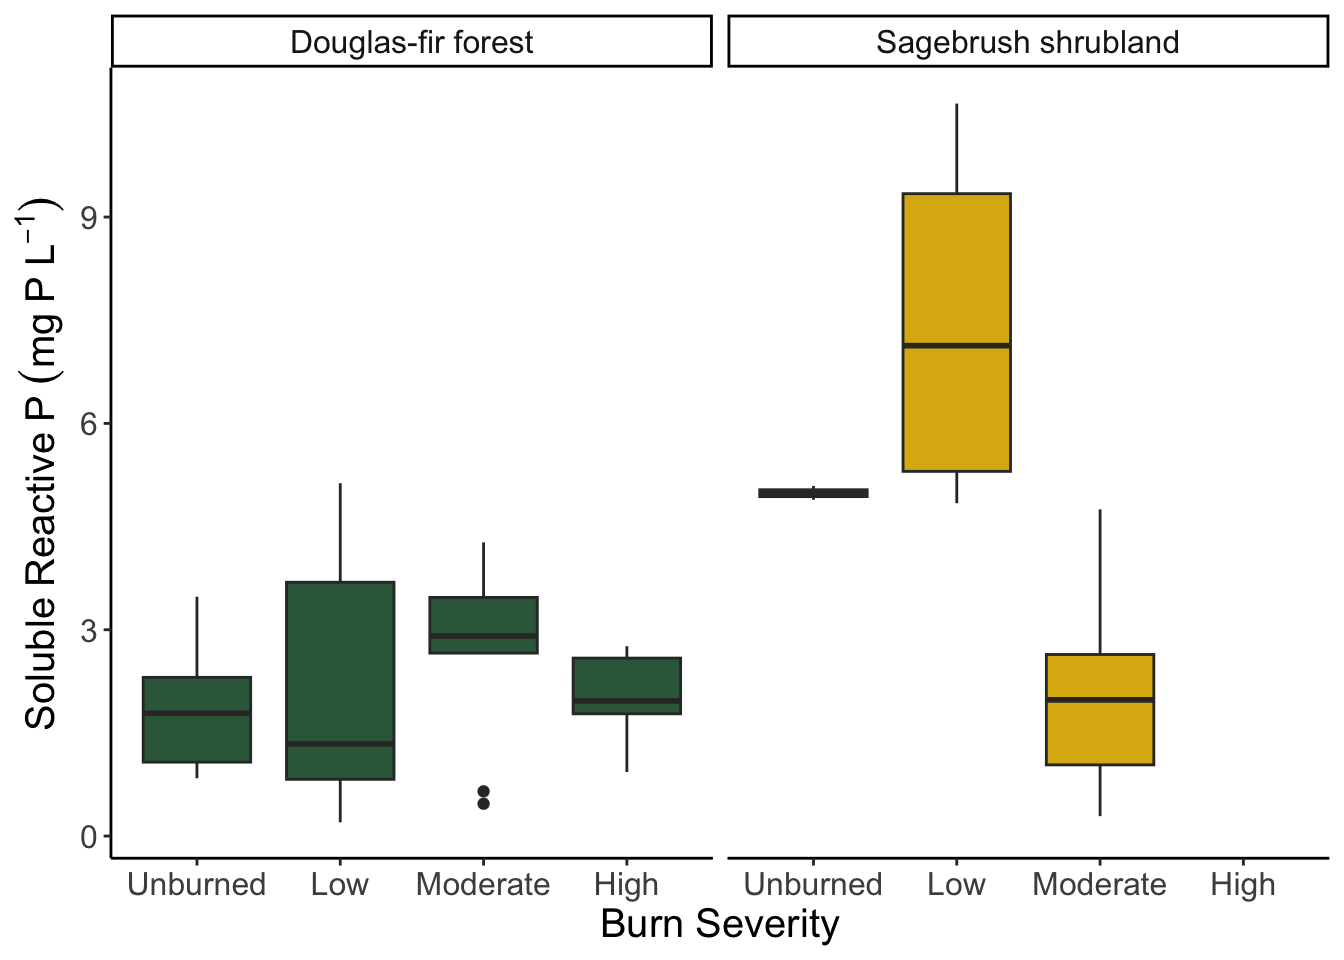
\includegraphics{BSLE_P_Code_Updated_files/figure-latex/MBD fig and stats-1.pdf}

\begin{Shaded}
\begin{Highlighting}[]
\CommentTok{\#MBD mg/kg figure; likely use this one for publication}
\NormalTok{MBD.BS.fig}\OtherTok{\textless{}{-}}\FunctionTok{ggplot}\NormalTok{(data, }\FunctionTok{aes}\NormalTok{(}\AttributeTok{x=}\NormalTok{Burn\_Severity, }\AttributeTok{y=}\NormalTok{MBD\_P\_mg\_kgchar}\SpecialCharTok{/}\DecValTok{1000}\NormalTok{, }\AttributeTok{fill=}\NormalTok{Land\_Coverage\_Category))}\SpecialCharTok{+}\FunctionTok{geom\_boxplot}\NormalTok{(}\AttributeTok{show.legend=}\ConstantTok{FALSE}\NormalTok{)}\SpecialCharTok{+}\FunctionTok{theme\_classic}\NormalTok{()}\SpecialCharTok{+}\FunctionTok{ylab}\NormalTok{(}\FunctionTok{expression}\NormalTok{(}\FunctionTok{paste}\NormalTok{(Soluble}\SpecialCharTok{\textasciitilde{}}\NormalTok{Reactive}\SpecialCharTok{\textasciitilde{}}\NormalTok{P}\SpecialCharTok{\textasciitilde{}}\NormalTok{(g}\SpecialCharTok{\textasciitilde{}}\NormalTok{P}\SpecialCharTok{\textasciitilde{}}\NormalTok{kg}\SpecialCharTok{\^{}{-}}\DecValTok{1}\NormalTok{), }\AttributeTok{sep=}\StringTok{""}\NormalTok{)))}\SpecialCharTok{+} \FunctionTok{xlab}\NormalTok{(}\StringTok{"Burn Severity"}\NormalTok{)}\SpecialCharTok{+}\FunctionTok{scale\_fill\_manual}\NormalTok{(}\AttributeTok{values=}\FunctionTok{c}\NormalTok{(}\StringTok{"\#346648"}\NormalTok{, }\StringTok{"\#dbb40d"}\NormalTok{))}\SpecialCharTok{+}\FunctionTok{facet\_grid}\NormalTok{(.}\SpecialCharTok{\textasciitilde{}}\NormalTok{Land\_Coverage\_Category)}\SpecialCharTok{+}\FunctionTok{theme}\NormalTok{(}\AttributeTok{text =} \FunctionTok{element\_text}\NormalTok{(}\AttributeTok{size =} \DecValTok{15}\NormalTok{))}

\NormalTok{cowplot}\SpecialCharTok{::}\FunctionTok{save\_plot}\NormalTok{(}\StringTok{"../figures/MBD.BS.fig.pdf"}\NormalTok{, MBD.BS.fig, }\AttributeTok{ncol =} \DecValTok{1}\NormalTok{, }\AttributeTok{nrow =} \DecValTok{1}\NormalTok{, }\AttributeTok{base\_aspect\_ratio=} \DecValTok{2}\SpecialCharTok{:}\DecValTok{1}\NormalTok{, }\AttributeTok{dpi=}\DecValTok{72}\NormalTok{)}
\end{Highlighting}
\end{Shaded}

\begin{verbatim}
## Warning: Removed 3 rows containing non-finite values (`stat_boxplot()`).
\end{verbatim}

\begin{Shaded}
\begin{Highlighting}[]
\CommentTok{\#MBD as percent of solid P concentration figure}
\FunctionTok{ggplot}\NormalTok{(data, }\FunctionTok{aes}\NormalTok{(}\AttributeTok{x=}\NormalTok{Burn\_Severity, }\AttributeTok{y=}\NormalTok{MBD\_P\_percentofsolid, }\AttributeTok{fill=}\NormalTok{Land\_Coverage\_Category))}\SpecialCharTok{+}\FunctionTok{geom\_boxplot}\NormalTok{(}\AttributeTok{show.legend=}\ConstantTok{FALSE}\NormalTok{)}\SpecialCharTok{+}\FunctionTok{theme\_classic}\NormalTok{()}\SpecialCharTok{+}\FunctionTok{ylab}\NormalTok{(}\StringTok{"Soluble Reactive P (\%)"}\NormalTok{)}\SpecialCharTok{+} \FunctionTok{xlab}\NormalTok{(}\StringTok{"Burn Severity"}\NormalTok{)}\SpecialCharTok{+}\FunctionTok{scale\_fill\_manual}\NormalTok{(}\AttributeTok{values=}\FunctionTok{c}\NormalTok{(}\StringTok{"\#346648"}\NormalTok{, }\StringTok{"\#dbb40d"}\NormalTok{))}\SpecialCharTok{+}\FunctionTok{facet\_grid}\NormalTok{(.}\SpecialCharTok{\textasciitilde{}}\NormalTok{Land\_Coverage\_Category)}\SpecialCharTok{+}\FunctionTok{theme}\NormalTok{(}\AttributeTok{text =} \FunctionTok{element\_text}\NormalTok{(}\AttributeTok{size =} \DecValTok{15}\NormalTok{))}
\end{Highlighting}
\end{Shaded}

\begin{verbatim}
## Warning: Removed 3 rows containing non-finite values (`stat_boxplot()`).
\end{verbatim}

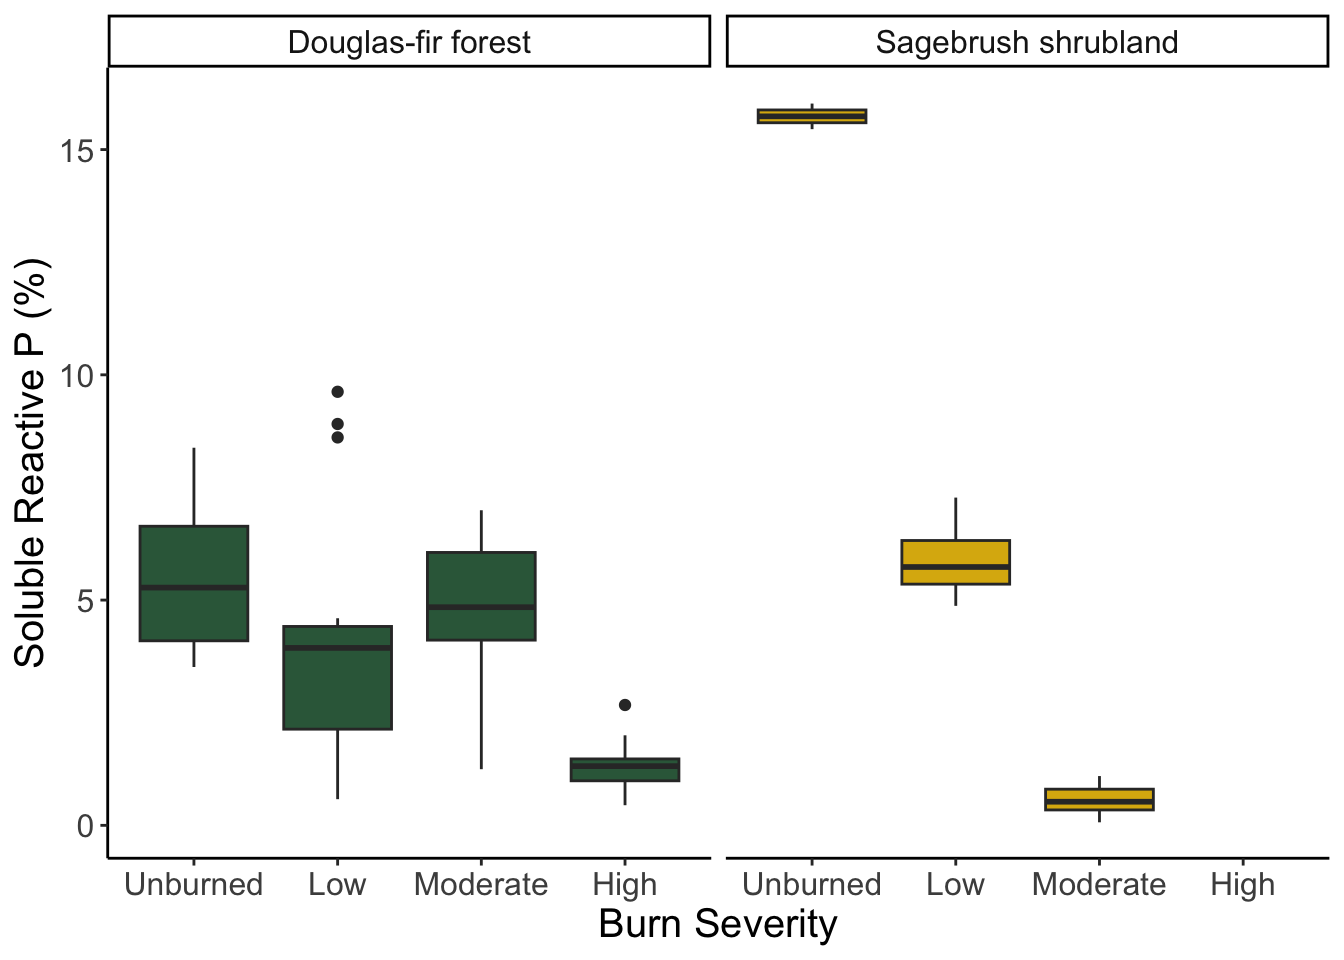
\includegraphics{BSLE_P_Code_Updated_files/figure-latex/MBD fig and stats-2.pdf}

\begin{Shaded}
\begin{Highlighting}[]
\CommentTok{\#MBD g/kg stats; likely use this one for publication}
\NormalTok{model}\OtherTok{\textless{}{-}}\FunctionTok{lmer}\NormalTok{(}\FunctionTok{log10}\NormalTok{(MBD\_P\_mg\_kgchar}\SpecialCharTok{/}\DecValTok{1000}\NormalTok{)}\SpecialCharTok{\textasciitilde{}}\NormalTok{Burn\_Severity}\SpecialCharTok{*}\NormalTok{Land\_Coverage\_Category}\SpecialCharTok{+}\NormalTok{(}\DecValTok{1}\SpecialCharTok{|}\NormalTok{Parent\_ID), }\AttributeTok{data=}\NormalTok{data) }\CommentTok{\#if want to use maximum likelihood , REML=FALSE}
\end{Highlighting}
\end{Shaded}

\begin{verbatim}
## fixed-effect model matrix is rank deficient so dropping 1 column / coefficient
\end{verbatim}

\begin{Shaded}
\begin{Highlighting}[]
\NormalTok{model.BS}\OtherTok{\textless{}{-}}\FunctionTok{lmer}\NormalTok{(}\FunctionTok{log10}\NormalTok{(MBD\_P\_mg\_kgchar}\SpecialCharTok{/}\DecValTok{1000}\NormalTok{)}\SpecialCharTok{\textasciitilde{}}\NormalTok{Land\_Coverage\_Category}\SpecialCharTok{+}\NormalTok{(}\DecValTok{1}\SpecialCharTok{|}\NormalTok{Parent\_ID), }\AttributeTok{data=}\NormalTok{data)}
\NormalTok{model.LC}\OtherTok{\textless{}{-}}\FunctionTok{lmer}\NormalTok{(}\FunctionTok{log10}\NormalTok{(MBD\_P\_mg\_kgchar}\SpecialCharTok{/}\DecValTok{1000}\NormalTok{)}\SpecialCharTok{\textasciitilde{}}\NormalTok{Burn\_Severity}\SpecialCharTok{+}\NormalTok{(}\DecValTok{1}\SpecialCharTok{|}\NormalTok{Parent\_ID), }\AttributeTok{data=}\NormalTok{data)}
\NormalTok{model.int}\OtherTok{\textless{}{-}}\FunctionTok{lmer}\NormalTok{(}\FunctionTok{log10}\NormalTok{(MBD\_P\_mg\_kgchar}\SpecialCharTok{/}\DecValTok{1000}\NormalTok{)}\SpecialCharTok{\textasciitilde{}}\NormalTok{Burn\_Severity}\SpecialCharTok{+}\NormalTok{Land\_Coverage\_Category}\SpecialCharTok{+}\NormalTok{(}\DecValTok{1}\SpecialCharTok{|}\NormalTok{Parent\_ID), }\AttributeTok{data=}\NormalTok{data)}
\FunctionTok{anova}\NormalTok{(model,model.BS) }\CommentTok{\#not sig}
\end{Highlighting}
\end{Shaded}

\begin{verbatim}
## refitting model(s) with ML (instead of REML)
\end{verbatim}

\begin{verbatim}
## Data: data
## Models:
## model.BS: log10(MBD_P_mg_kgchar/1000) ~ Land_Coverage_Category + (1 | Parent_ID)
## model: log10(MBD_P_mg_kgchar/1000) ~ Burn_Severity * Land_Coverage_Category + (1 | Parent_ID)
##          npar    AIC    BIC   logLik deviance Chisq Df Pr(>Chisq)
## model.BS    4 30.181 38.137 -11.0905   22.181                    
## model       9 32.325 50.226  -7.1625   14.325 7.856  5     0.1644
\end{verbatim}

\begin{Shaded}
\begin{Highlighting}[]
\FunctionTok{anova}\NormalTok{(model,model.LC) }\CommentTok{\#sig}
\end{Highlighting}
\end{Shaded}

\begin{verbatim}
## refitting model(s) with ML (instead of REML)
\end{verbatim}

\begin{verbatim}
## Data: data
## Models:
## model.LC: log10(MBD_P_mg_kgchar/1000) ~ Burn_Severity + (1 | Parent_ID)
## model: log10(MBD_P_mg_kgchar/1000) ~ Burn_Severity * Land_Coverage_Category + (1 | Parent_ID)
##          npar    AIC    BIC   logLik deviance  Chisq Df Pr(>Chisq)  
## model.LC    6 37.291 49.225 -12.6453   25.291                       
## model       9 32.325 50.226  -7.1625   14.325 10.966  3    0.01191 *
## ---
## Signif. codes:  0 '***' 0.001 '**' 0.01 '*' 0.05 '.' 0.1 ' ' 1
\end{verbatim}

\begin{Shaded}
\begin{Highlighting}[]
\FunctionTok{anova}\NormalTok{(model,model.int) }\CommentTok{\#sig}
\end{Highlighting}
\end{Shaded}

\begin{verbatim}
## refitting model(s) with ML (instead of REML)
\end{verbatim}

\begin{verbatim}
## Data: data
## Models:
## model.int: log10(MBD_P_mg_kgchar/1000) ~ Burn_Severity + Land_Coverage_Category + (1 | Parent_ID)
## model: log10(MBD_P_mg_kgchar/1000) ~ Burn_Severity * Land_Coverage_Category + (1 | Parent_ID)
##           npar    AIC    BIC   logLik deviance  Chisq Df Pr(>Chisq)  
## model.int    7 35.410 49.333 -10.7051   21.410                       
## model        9 32.325 50.226  -7.1625   14.325 7.0852  2    0.02894 *
## ---
## Signif. codes:  0 '***' 0.001 '**' 0.01 '*' 0.05 '.' 0.1 ' ' 1
\end{verbatim}

\begin{Shaded}
\begin{Highlighting}[]
\CommentTok{\#check VIF}
\FunctionTok{vif}\NormalTok{(model)}
\end{Highlighting}
\end{Shaded}

\begin{verbatim}
##                                          GVIF Df GVIF^(1/(2*Df))
## Burn_Severity                        2.567759  3        1.170197
## Land_Coverage_Category               5.502341  1        2.345707
## Burn_Severity:Land_Coverage_Category 9.075768  2        1.735685
\end{verbatim}

\begin{Shaded}
\begin{Highlighting}[]
\CommentTok{\#model assumptions}
\FunctionTok{hist}\NormalTok{(}\FunctionTok{log10}\NormalTok{(data}\SpecialCharTok{$}\NormalTok{MBD\_P\_mg\_kgchar))}
\end{Highlighting}
\end{Shaded}

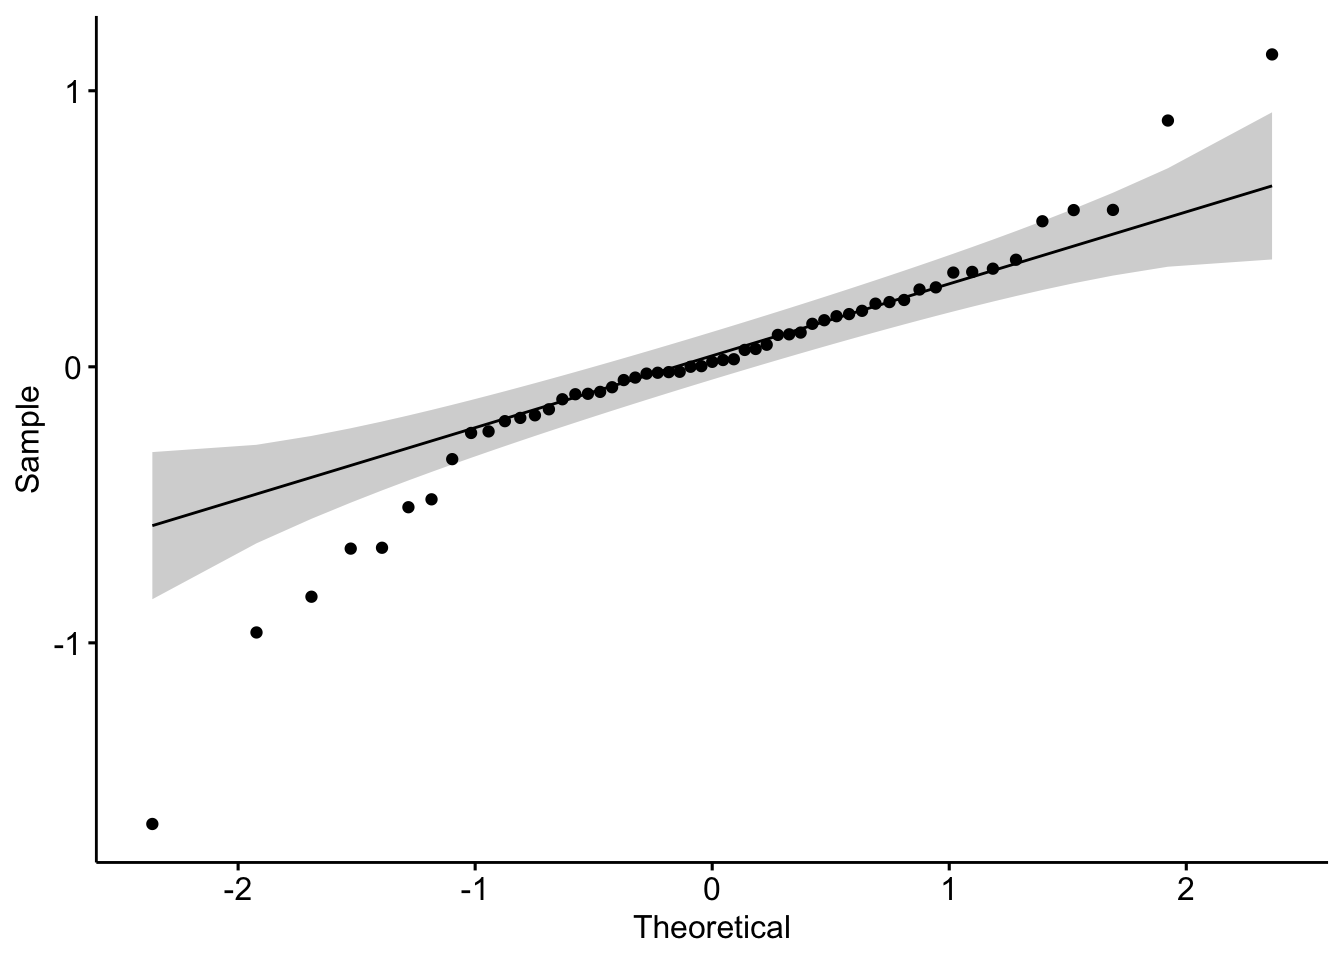
\includegraphics{BSLE_P_Code_Updated_files/figure-latex/MBD fig and stats-3.pdf}

\begin{Shaded}
\begin{Highlighting}[]
\CommentTok{\#linearity}
\FunctionTok{ggqqplot}\NormalTok{(}\FunctionTok{residuals}\NormalTok{(model))}
\end{Highlighting}
\end{Shaded}

\includegraphics{BSLE_P_Code_Updated_files/figure-latex/MBD fig and stats-4.pdf}

\begin{Shaded}
\begin{Highlighting}[]
\CommentTok{\#check normality of residuals }
\FunctionTok{shapiro.test}\NormalTok{(}\FunctionTok{log10}\NormalTok{(data}\SpecialCharTok{$}\NormalTok{MBD\_P\_mg\_kgchar)) }\CommentTok{\#p \textgreater{} 0.05 so can assume normality }
\end{Highlighting}
\end{Shaded}

\begin{verbatim}
## 
##  Shapiro-Wilk normality test
## 
## data:  log10(data$MBD_P_mg_kgchar)
## W = 0.95892, p-value = 0.06167
\end{verbatim}

\begin{Shaded}
\begin{Highlighting}[]
\CommentTok{\#check homogeneity of variance assumption (homoscedastcity)}
\FunctionTok{plot}\NormalTok{(}\FunctionTok{fitted}\NormalTok{(model),}\FunctionTok{residuals}\NormalTok{(model))}
\end{Highlighting}
\end{Shaded}

\includegraphics{BSLE_P_Code_Updated_files/figure-latex/MBD fig and stats-5.pdf}

\begin{Shaded}
\begin{Highlighting}[]
\NormalTok{performance}\SpecialCharTok{::}\FunctionTok{check\_heteroscedasticity}\NormalTok{(model) }\CommentTok{\#p \textgreater{} 0.05 so can assume homoscedastic}
\end{Highlighting}
\end{Shaded}

\begin{verbatim}
## OK: Error variance appears to be homoscedastic (p = 0.632).
\end{verbatim}

\begin{Shaded}
\begin{Highlighting}[]
\CommentTok{\#post hoc tests for interaction term}
\NormalTok{emmeans}\SpecialCharTok{::}\FunctionTok{lsmeans}\NormalTok{(model, pairwise}\SpecialCharTok{\textasciitilde{}}\NormalTok{Burn\_Severity}\SpecialCharTok{*}\NormalTok{Land\_Coverage\_Category, }\AttributeTok{at=}\FunctionTok{list}\NormalTok{(}\AttributeTok{Burn\_Severity=}\StringTok{"Unburned"}\NormalTok{),}\AttributeTok{adjust=}\StringTok{"tukey"}\NormalTok{)}
\end{Highlighting}
\end{Shaded}

\begin{verbatim}
## $lsmeans
##  Burn_Severity Land_Coverage_Category lsmean    SE   df lower.CL upper.CL
##  Unburned      Douglas-fir forest     -1.183 0.221 11.7    -1.67  -0.6994
##  Unburned      Sagebrush shrubland    -0.701 0.313 11.7    -1.39  -0.0163
## 
## Degrees-of-freedom method: kenward-roger 
## Results are given on the log10 (not the response) scale. 
## Confidence level used: 0.95 
## 
## $contrasts
##  contrast                                                     estimate    SE
##  (Unburned Douglas-fir forest) - Unburned Sagebrush shrubland   -0.483 0.384
##    df t.ratio p.value
##  11.7  -1.258  0.2328
## 
## Degrees-of-freedom method: kenward-roger 
## Results are given on the log10 (not the response) scale.
\end{verbatim}

\begin{Shaded}
\begin{Highlighting}[]
\NormalTok{emmeans}\SpecialCharTok{::}\FunctionTok{lsmeans}\NormalTok{(model, pairwise}\SpecialCharTok{\textasciitilde{}}\NormalTok{Burn\_Severity}\SpecialCharTok{*}\NormalTok{Land\_Coverage\_Category, }\AttributeTok{at=}\FunctionTok{list}\NormalTok{(}\AttributeTok{Burn\_Severity=}\StringTok{"Low"}\NormalTok{),}\AttributeTok{adjust=}\StringTok{"tukey"}\NormalTok{)}
\end{Highlighting}
\end{Shaded}

\begin{verbatim}
## $lsmeans
##  Burn_Severity Land_Coverage_Category lsmean    SE   df lower.CL upper.CL
##  Low           Douglas-fir forest     -1.266 0.140 11.7    -1.57   -0.960
##  Low           Sagebrush shrubland    -0.551 0.221 11.7    -1.03   -0.067
## 
## Degrees-of-freedom method: kenward-roger 
## Results are given on the log10 (not the response) scale. 
## Confidence level used: 0.95 
## 
## $contrasts
##  contrast                                           estimate    SE   df t.ratio
##  (Low Douglas-fir forest) - Low Sagebrush shrubland   -0.715 0.262 11.7  -2.729
##  p.value
##   0.0187
## 
## Degrees-of-freedom method: kenward-roger 
## Results are given on the log10 (not the response) scale.
\end{verbatim}

\begin{Shaded}
\begin{Highlighting}[]
\NormalTok{emmeans}\SpecialCharTok{::}\FunctionTok{lsmeans}\NormalTok{(model, pairwise}\SpecialCharTok{\textasciitilde{}}\NormalTok{Burn\_Severity}\SpecialCharTok{*}\NormalTok{Land\_Coverage\_Category, }\AttributeTok{at=}\FunctionTok{list}\NormalTok{(}\AttributeTok{Burn\_Severity=}\StringTok{"Moderate"}\NormalTok{),}\AttributeTok{adjust=}\StringTok{"tukey"}\NormalTok{)}
\end{Highlighting}
\end{Shaded}

\begin{verbatim}
## $lsmeans
##  Burn_Severity Land_Coverage_Category lsmean    SE   df lower.CL upper.CL
##  Moderate      Douglas-fir forest      -1.05 0.181 11.7    -1.45   -0.655
##  Moderate      Sagebrush shrubland     -1.23 0.221 11.7    -1.71   -0.742
## 
## Degrees-of-freedom method: kenward-roger 
## Results are given on the log10 (not the response) scale. 
## Confidence level used: 0.95 
## 
## $contrasts
##  contrast                                                     estimate    SE
##  (Moderate Douglas-fir forest) - Moderate Sagebrush shrubland    0.176 0.286
##    df t.ratio p.value
##  11.7   0.616  0.5500
## 
## Degrees-of-freedom method: kenward-roger 
## Results are given on the log10 (not the response) scale.
\end{verbatim}

\begin{Shaded}
\begin{Highlighting}[]
\NormalTok{emmeans}\SpecialCharTok{::}\FunctionTok{lsmeans}\NormalTok{(model, pairwise}\SpecialCharTok{\textasciitilde{}}\NormalTok{Burn\_Severity}\SpecialCharTok{*}\NormalTok{Land\_Coverage\_Category, }\AttributeTok{at=}\FunctionTok{list}\NormalTok{(}\AttributeTok{Land\_Coverage\_Category=}\StringTok{"Douglas{-}fir forest"}\NormalTok{),}\AttributeTok{adjust=}\StringTok{"tukey"}\NormalTok{)}
\end{Highlighting}
\end{Shaded}

\begin{verbatim}
## $lsmeans
##  Burn_Severity Land_Coverage_Category lsmean    SE   df lower.CL upper.CL
##  High          Douglas-fir forest      -1.07 0.161 13.1    -1.42   -0.726
##  Low           Douglas-fir forest      -1.27 0.140 11.7    -1.57   -0.960
##  Moderate      Douglas-fir forest      -1.05 0.181 11.7    -1.45   -0.655
##  Unburned      Douglas-fir forest      -1.18 0.221 11.7    -1.67   -0.699
## 
## Degrees-of-freedom method: kenward-roger 
## Results are given on the log10 (not the response) scale. 
## Confidence level used: 0.95 
## 
## $contrasts
##  contrast                                                      estimate    SE
##  (High Douglas-fir forest) - (Low Douglas-fir forest)            0.1918 0.214
##  (High Douglas-fir forest) - (Moderate Douglas-fir forest)      -0.0238 0.242
##  (High Douglas-fir forest) - (Unburned Douglas-fir forest)       0.1093 0.274
##  (Low Douglas-fir forest) - (Moderate Douglas-fir forest)       -0.2156 0.229
##  (Low Douglas-fir forest) - (Unburned Douglas-fir forest)       -0.0825 0.262
##  (Moderate Douglas-fir forest) - (Unburned Douglas-fir forest)   0.1331 0.286
##    df t.ratio p.value
##  12.4   0.898  0.8062
##  12.3  -0.098  0.9996
##  12.1   0.399  0.9775
##  11.7  -0.943  0.7830
##  11.7  -0.315  0.9886
##  11.7   0.466  0.9651
## 
## Degrees-of-freedom method: kenward-roger 
## Results are given on the log10 (not the response) scale. 
## P value adjustment: tukey method for comparing a family of 4 estimates
\end{verbatim}

\begin{Shaded}
\begin{Highlighting}[]
\NormalTok{emmeans}\SpecialCharTok{::}\FunctionTok{lsmeans}\NormalTok{(model, pairwise}\SpecialCharTok{\textasciitilde{}}\NormalTok{Burn\_Severity}\SpecialCharTok{*}\NormalTok{Land\_Coverage\_Category, }\AttributeTok{at=}\FunctionTok{list}\NormalTok{(}\AttributeTok{Land\_Coverage\_Category=}\StringTok{"Sagebrush shrubland"}\NormalTok{),}\AttributeTok{adjust=}\StringTok{"tukey"}\NormalTok{)}
\end{Highlighting}
\end{Shaded}

\begin{verbatim}
## $lsmeans
##  Burn_Severity Land_Coverage_Category lsmean    SE   df lower.CL upper.CL
##  High          Sagebrush shrubland    nonEst    NA   NA       NA       NA
##  Low           Sagebrush shrubland    -0.551 0.221 11.7    -1.03  -0.0670
##  Moderate      Sagebrush shrubland    -1.226 0.221 11.7    -1.71  -0.7423
##  Unburned      Sagebrush shrubland    -0.701 0.313 11.7    -1.39  -0.0163
## 
## Degrees-of-freedom method: kenward-roger 
## Results are given on the log10 (not the response) scale. 
## Confidence level used: 0.95 
## 
## $contrasts
##  contrast                                                    estimate    SE
##  High Sagebrush shrubland - Low Sagebrush shrubland            nonEst    NA
##  High Sagebrush shrubland - Moderate Sagebrush shrubland       nonEst    NA
##  High Sagebrush shrubland - Unburned Sagebrush shrubland       nonEst    NA
##  Low Sagebrush shrubland - Moderate Sagebrush shrubland         0.675 0.313
##  Low Sagebrush shrubland - Unburned Sagebrush shrubland         0.150 0.384
##  Moderate Sagebrush shrubland - Unburned Sagebrush shrubland   -0.526 0.384
##    df t.ratio p.value
##    NA      NA      NA
##    NA      NA      NA
##    NA      NA      NA
##  11.7   2.157  0.1908
##  11.7   0.391  0.9788
##  11.7  -1.370  0.5396
## 
## Degrees-of-freedom method: kenward-roger 
## Results are given on the log10 (not the response) scale. 
## P value adjustment: tukey method for comparing a family of 4 estimates
\end{verbatim}

\#\#\#\#ICP Leachates

\begin{Shaded}
\begin{Highlighting}[]
\CommentTok{\#convert to percent of total P in unfiltered sample}
\CommentTok{\#ICP$P.filt.percentofunfilt\textless{}{-}(ICP$Total\_P\_mg\_per\_L\_filt/ICP$Total\_P\_mg\_per\_L\_unfilt)*100}
\CommentTok{\#ICP$P.part.percentofunfilt\textless{}{-}(ICP$Total\_P\_mg\_per\_L\_part/ICP$Total\_P\_mg\_per\_L\_unfilt)*100}

\CommentTok{\#total P in unfiltered leachate}
\NormalTok{Leachate.total.P.BS.boxplot }\OtherTok{\textless{}{-}} \FunctionTok{ggplot}\NormalTok{(data, }\FunctionTok{aes}\NormalTok{(}\AttributeTok{x=}\NormalTok{Burn\_Severity, }\AttributeTok{y=}\NormalTok{Leachate\_P\_mg\_kgchar\_unfilt, }\AttributeTok{fill=}\NormalTok{Land\_Coverage\_Category))}\SpecialCharTok{+}\FunctionTok{geom\_boxplot}\NormalTok{(}\AttributeTok{show.legend=}\ConstantTok{FALSE}\NormalTok{)}\SpecialCharTok{+}\FunctionTok{theme\_classic}\NormalTok{()}\SpecialCharTok{+}\FunctionTok{ylab}\NormalTok{(}\FunctionTok{expression}\NormalTok{(}\FunctionTok{paste}\NormalTok{(Total}\SpecialCharTok{\textasciitilde{}}\NormalTok{P}\SpecialCharTok{\textasciitilde{}}\NormalTok{(mg}\SpecialCharTok{\textasciitilde{}}\NormalTok{P}\SpecialCharTok{\textasciitilde{}}\NormalTok{kg}\SpecialCharTok{\^{}{-}}\DecValTok{1}\NormalTok{), }\AttributeTok{sep=}\StringTok{""}\NormalTok{)))}\SpecialCharTok{+} \FunctionTok{xlab}\NormalTok{(}\StringTok{"Burn Severity"}\NormalTok{)}\SpecialCharTok{+}\FunctionTok{scale\_fill\_manual}\NormalTok{(}\AttributeTok{values=}\FunctionTok{c}\NormalTok{(}\StringTok{"\#346648"}\NormalTok{, }\StringTok{"\#dbb40d"}\NormalTok{))}\SpecialCharTok{+}\FunctionTok{facet\_grid}\NormalTok{(.}\SpecialCharTok{\textasciitilde{}}\NormalTok{Land\_Coverage\_Category)}\SpecialCharTok{+}\FunctionTok{theme}\NormalTok{(}\AttributeTok{text =} \FunctionTok{element\_text}\NormalTok{(}\AttributeTok{size =} \DecValTok{15}\NormalTok{))}

\NormalTok{cowplot}\SpecialCharTok{::}\FunctionTok{save\_plot}\NormalTok{(}\StringTok{"../figures/Leachate.total.P.BS.boxplot.pdf"}\NormalTok{, Leachate.total.P.BS.boxplot, }\AttributeTok{ncol =} \DecValTok{1}\NormalTok{, }\AttributeTok{nrow =} \DecValTok{1}\NormalTok{, }\AttributeTok{base\_aspect\_ratio=} \DecValTok{2}\SpecialCharTok{:}\DecValTok{1}\NormalTok{, }\AttributeTok{dpi=}\DecValTok{72}\NormalTok{)}

\NormalTok{Leachate.filt0.}\FloatTok{7.}\NormalTok{total.P.BS.boxplot }\OtherTok{\textless{}{-}} \FunctionTok{ggplot}\NormalTok{(data, }\FunctionTok{aes}\NormalTok{(}\AttributeTok{x=}\NormalTok{Burn\_Severity, }\AttributeTok{y=}\NormalTok{Leachate\_P\_mg\_kgchar\_filt0}\FloatTok{.7}\NormalTok{, }\AttributeTok{fill=}\NormalTok{Land\_Coverage\_Category))}\SpecialCharTok{+}\FunctionTok{geom\_boxplot}\NormalTok{(}\AttributeTok{show.legend=}\ConstantTok{FALSE}\NormalTok{)}\SpecialCharTok{+}\FunctionTok{theme\_classic}\NormalTok{()}\SpecialCharTok{+}\FunctionTok{ylab}\NormalTok{(}\FunctionTok{expression}\NormalTok{(}\FunctionTok{paste}\NormalTok{(Total}\SpecialCharTok{\textasciitilde{}}\NormalTok{Soluble}\SpecialCharTok{\textasciitilde{}}\NormalTok{P}\SpecialCharTok{\textasciitilde{}}\NormalTok{(mg}\SpecialCharTok{\textasciitilde{}}\NormalTok{P}\SpecialCharTok{\textasciitilde{}}\NormalTok{kg}\SpecialCharTok{\^{}{-}}\DecValTok{1}\NormalTok{), }\AttributeTok{sep=}\StringTok{""}\NormalTok{)))}\SpecialCharTok{+} \FunctionTok{xlab}\NormalTok{(}\StringTok{"Burn Severity"}\NormalTok{)}\SpecialCharTok{+}\FunctionTok{scale\_fill\_manual}\NormalTok{(}\AttributeTok{values=}\FunctionTok{c}\NormalTok{(}\StringTok{"\#346648"}\NormalTok{, }\StringTok{"\#dbb40d"}\NormalTok{))}\SpecialCharTok{+}\FunctionTok{facet\_grid}\NormalTok{(.}\SpecialCharTok{\textasciitilde{}}\NormalTok{Land\_Coverage\_Category)}\SpecialCharTok{+}\FunctionTok{theme}\NormalTok{(}\AttributeTok{text =} \FunctionTok{element\_text}\NormalTok{(}\AttributeTok{size =} \DecValTok{15}\NormalTok{))}

\NormalTok{cowplot}\SpecialCharTok{::}\FunctionTok{save\_plot}\NormalTok{(}\StringTok{"../figures/Leachate.filt0.7.total.P.BS.boxplot.pdf"}\NormalTok{, Leachate.filt0.}\FloatTok{7.}\NormalTok{total.P.BS.boxplot, }\AttributeTok{ncol =} \DecValTok{1}\NormalTok{, }\AttributeTok{nrow =} \DecValTok{1}\NormalTok{, }\AttributeTok{base\_aspect\_ratio=} \DecValTok{2}\SpecialCharTok{:}\DecValTok{1}\NormalTok{, }\AttributeTok{dpi=}\DecValTok{72}\NormalTok{)}

\NormalTok{Leachate.unfilt.total.P.BS.boxplot }\OtherTok{\textless{}{-}} \FunctionTok{ggplot}\NormalTok{(data, }\FunctionTok{aes}\NormalTok{(}\AttributeTok{x=}\NormalTok{Burn\_Severity, }\AttributeTok{y=}\NormalTok{Leachate\_P\_mg\_kgchar\_part, }\AttributeTok{fill=}\NormalTok{Land\_Coverage\_Category))}\SpecialCharTok{+}\FunctionTok{geom\_boxplot}\NormalTok{(}\AttributeTok{show.legend=}\ConstantTok{FALSE}\NormalTok{)}\SpecialCharTok{+}\FunctionTok{theme\_classic}\NormalTok{()}\SpecialCharTok{+}\FunctionTok{ylab}\NormalTok{(}\FunctionTok{expression}\NormalTok{(}\FunctionTok{paste}\NormalTok{(Total}\SpecialCharTok{\textasciitilde{}}\NormalTok{Particulate}\SpecialCharTok{\textasciitilde{}}\NormalTok{P}\SpecialCharTok{\textasciitilde{}}\NormalTok{(mg}\SpecialCharTok{\textasciitilde{}}\NormalTok{P}\SpecialCharTok{\textasciitilde{}}\NormalTok{kg}\SpecialCharTok{\^{}{-}}\DecValTok{1}\NormalTok{), }\AttributeTok{sep=}\StringTok{""}\NormalTok{)))}\SpecialCharTok{+} \FunctionTok{xlab}\NormalTok{(}\StringTok{"Burn Severity"}\NormalTok{)}\SpecialCharTok{+}\FunctionTok{scale\_fill\_manual}\NormalTok{(}\AttributeTok{values=}\FunctionTok{c}\NormalTok{(}\StringTok{"\#346648"}\NormalTok{, }\StringTok{"\#dbb40d"}\NormalTok{))}\SpecialCharTok{+}\FunctionTok{facet\_grid}\NormalTok{(.}\SpecialCharTok{\textasciitilde{}}\NormalTok{Land\_Coverage\_Category)}\SpecialCharTok{+}\FunctionTok{theme}\NormalTok{(}\AttributeTok{text =} \FunctionTok{element\_text}\NormalTok{(}\AttributeTok{size =} \DecValTok{15}\NormalTok{))}

\NormalTok{cowplot}\SpecialCharTok{::}\FunctionTok{save\_plot}\NormalTok{(}\StringTok{"../figures/Leachate.unfilt.total.P.BS.boxplot.pdf"}\NormalTok{, Leachate.unfilt.total.P.BS.boxplot, }\AttributeTok{ncol =} \DecValTok{1}\NormalTok{, }\AttributeTok{nrow =} \DecValTok{1}\NormalTok{, }\AttributeTok{base\_aspect\_ratio=} \DecValTok{2}\SpecialCharTok{:}\DecValTok{1}\NormalTok{, }\AttributeTok{dpi=}\DecValTok{72}\NormalTok{)}


\CommentTok{\#stacked bar chart}
\NormalTok{P.Conc.leach.bar }\OtherTok{\textless{}{-}}\NormalTok{ P.Conc.leach }\SpecialCharTok{\%\textgreater{}\%}
  \FunctionTok{mutate}\NormalTok{(}\AttributeTok{sd.high=}\NormalTok{Leachate\_P\_mg\_kgchar\_unfilt\_Mean}\SpecialCharTok{+}\NormalTok{Leachate\_P\_mg\_kgchar\_unfilt\_Standard\_Deviation) }\SpecialCharTok{\%\textgreater{}\%}
  \FunctionTok{mutate}\NormalTok{(}\AttributeTok{sd.low=}\NormalTok{Leachate\_P\_mg\_kgchar\_unfilt\_Mean}\SpecialCharTok{{-}}\NormalTok{Leachate\_P\_mg\_kgchar\_unfilt\_Standard\_Deviation)}


\NormalTok{P.Conc.leach\_melt}\OtherTok{\textless{}{-}}\FunctionTok{melt}\NormalTok{(P.Conc.leach.bar, }\AttributeTok{id=}\FunctionTok{c}\NormalTok{(}\StringTok{"Burn\_Severity"}\NormalTok{, }\StringTok{"Land\_Coverage\_Category"}\NormalTok{,}\StringTok{"sd.low"}\NormalTok{, }\StringTok{"sd.high"}\NormalTok{)) }\SpecialCharTok{\%\textgreater{}\%}
  \FunctionTok{filter}\NormalTok{(variable }\SpecialCharTok{\%in\%} \FunctionTok{c}\NormalTok{(}\StringTok{"Leachate\_P\_mg\_kgchar\_part\_Mean"}\NormalTok{ , }\StringTok{"Leachate\_P\_mg\_kgchar\_filt0.7\_Mean"}\NormalTok{))}


\NormalTok{Leachate\_stacked\_bar }\OtherTok{\textless{}{-}} \FunctionTok{ggplot}\NormalTok{(}\FunctionTok{subset}\NormalTok{(P.Conc.leach\_melt, variable}\SpecialCharTok{==}\StringTok{"Leachate\_P\_mg\_kgchar\_part\_Mean"} \SpecialCharTok{|}\NormalTok{ variable}\SpecialCharTok{==}\StringTok{"Leachate\_P\_mg\_kgchar\_filt0.7\_Mean"}\NormalTok{), }\FunctionTok{aes}\NormalTok{(}\AttributeTok{x =}\NormalTok{ Burn\_Severity, }\AttributeTok{y =}\NormalTok{ value, }\AttributeTok{fill=}\NormalTok{variable)) }\SpecialCharTok{+} \FunctionTok{geom\_bar}\NormalTok{(}\AttributeTok{stat =} \StringTok{"identity"}\NormalTok{)  }\SpecialCharTok{+} \FunctionTok{theme\_classic}\NormalTok{()}\SpecialCharTok{+}\FunctionTok{ylab}\NormalTok{(}\FunctionTok{expression}\NormalTok{(}\FunctionTok{paste}\NormalTok{(Leachate}\SpecialCharTok{\textasciitilde{}}\NormalTok{Mean}\SpecialCharTok{\textasciitilde{}}\NormalTok{Total}\SpecialCharTok{\textasciitilde{}}\NormalTok{P}\SpecialCharTok{\textasciitilde{}}\NormalTok{(mg}\SpecialCharTok{\textasciitilde{}}\NormalTok{P}\SpecialCharTok{\textasciitilde{}}\NormalTok{kg}\SpecialCharTok{\^{}{-}}\DecValTok{1}\NormalTok{), }\AttributeTok{sep=}\StringTok{""}\NormalTok{)))}\SpecialCharTok{+} \FunctionTok{xlab}\NormalTok{(}\StringTok{"Burn Severity"}\NormalTok{)}\SpecialCharTok{+}\FunctionTok{scale\_fill\_manual}\NormalTok{(}\AttributeTok{values=}\FunctionTok{c}\NormalTok{(}\StringTok{"\#2274A5"}\NormalTok{, }\StringTok{"\#E7DFC6"}\NormalTok{), }\AttributeTok{labels =} \FunctionTok{c}\NormalTok{(}\StringTok{"Particulate"}\NormalTok{, }\StringTok{"Soluble"}\NormalTok{), }\AttributeTok{name =} \StringTok{""}\NormalTok{)}\SpecialCharTok{+}\FunctionTok{facet\_grid}\NormalTok{(.}\SpecialCharTok{\textasciitilde{}}\NormalTok{Land\_Coverage\_Category)}\SpecialCharTok{+}\FunctionTok{theme}\NormalTok{(}\AttributeTok{text =} \FunctionTok{element\_text}\NormalTok{(}\AttributeTok{size =} \DecValTok{15}\NormalTok{)) }\SpecialCharTok{+} \FunctionTok{geom\_errorbar}\NormalTok{(}\FunctionTok{aes}\NormalTok{(}\AttributeTok{ymax=}\NormalTok{sd.high, }\AttributeTok{ymin=}\NormalTok{sd.low), }\AttributeTok{width =} \FloatTok{0.2}\NormalTok{, }\AttributeTok{size =} \DecValTok{1}\NormalTok{, }\AttributeTok{color =} \StringTok{"black"}\NormalTok{)}
\end{Highlighting}
\end{Shaded}

\begin{verbatim}
## Warning: Using `size` aesthetic for lines was deprecated in ggplot2 3.4.0.
## i Please use `linewidth` instead.
## This warning is displayed once every 8 hours.
## Call `lifecycle::last_lifecycle_warnings()` to see where this warning was
## generated.
\end{verbatim}

\begin{Shaded}
\begin{Highlighting}[]
\NormalTok{cowplot}\SpecialCharTok{::}\FunctionTok{save\_plot}\NormalTok{(}\StringTok{"../figures/Leachate\_stacked\_bar.pdf"}\NormalTok{, Leachate\_stacked\_bar, }\AttributeTok{ncol =} \DecValTok{1}\NormalTok{, }\AttributeTok{nrow =} \DecValTok{1}\NormalTok{, }\AttributeTok{base\_aspect\_ratio=} \DecValTok{2}\SpecialCharTok{:}\DecValTok{1}\NormalTok{, }\AttributeTok{dpi=}\DecValTok{72}\NormalTok{)}


\CommentTok{\#ICP unfiltered total P g/kg stats; likely use this one for publication}
\NormalTok{model}\OtherTok{\textless{}{-}}\FunctionTok{lmer}\NormalTok{(}\FunctionTok{log10}\NormalTok{(Leachate\_P\_mg\_kgchar\_unfilt}\SpecialCharTok{/}\DecValTok{1000}\NormalTok{)}\SpecialCharTok{\textasciitilde{}}\NormalTok{Burn\_Severity}\SpecialCharTok{*}\NormalTok{Land\_Coverage\_Category}\SpecialCharTok{+}\NormalTok{(}\DecValTok{1}\SpecialCharTok{|}\NormalTok{Parent\_ID), }\AttributeTok{data=}\NormalTok{data)}
\end{Highlighting}
\end{Shaded}

\begin{verbatim}
## fixed-effect model matrix is rank deficient so dropping 1 column / coefficient
\end{verbatim}

\begin{Shaded}
\begin{Highlighting}[]
\NormalTok{model.BS}\OtherTok{\textless{}{-}}\FunctionTok{lmer}\NormalTok{(}\FunctionTok{log10}\NormalTok{(Leachate\_P\_mg\_kgchar\_unfilt}\SpecialCharTok{/}\DecValTok{1000}\NormalTok{)}\SpecialCharTok{\textasciitilde{}}\NormalTok{Land\_Coverage\_Category}\SpecialCharTok{+}\NormalTok{(}\DecValTok{1}\SpecialCharTok{|}\NormalTok{Parent\_ID), }\AttributeTok{data=}\NormalTok{data)}
\NormalTok{model.LC}\OtherTok{\textless{}{-}}\FunctionTok{lmer}\NormalTok{(}\FunctionTok{log10}\NormalTok{(Leachate\_P\_mg\_kgchar\_unfilt}\SpecialCharTok{/}\DecValTok{1000}\NormalTok{)}\SpecialCharTok{\textasciitilde{}}\NormalTok{Burn\_Severity}\SpecialCharTok{+}\NormalTok{(}\DecValTok{1}\SpecialCharTok{|}\NormalTok{Parent\_ID), }\AttributeTok{data=}\NormalTok{data)}
\NormalTok{model.int}\OtherTok{\textless{}{-}}\FunctionTok{lmer}\NormalTok{(}\FunctionTok{log10}\NormalTok{(Leachate\_P\_mg\_kgchar\_unfilt}\SpecialCharTok{/}\DecValTok{1000}\NormalTok{)}\SpecialCharTok{\textasciitilde{}}\NormalTok{Burn\_Severity}\SpecialCharTok{+}\NormalTok{Land\_Coverage\_Category}\SpecialCharTok{+}\NormalTok{(}\DecValTok{1}\SpecialCharTok{|}\NormalTok{Parent\_ID), }\AttributeTok{data=}\NormalTok{data)}
\FunctionTok{anova}\NormalTok{(model,model.BS)}
\end{Highlighting}
\end{Shaded}

\begin{verbatim}
## refitting model(s) with ML (instead of REML)
\end{verbatim}

\begin{verbatim}
## Data: data
## Models:
## model.BS: log10(Leachate_P_mg_kgchar_unfilt/1000) ~ Land_Coverage_Category + (1 | Parent_ID)
## model: log10(Leachate_P_mg_kgchar_unfilt/1000) ~ Burn_Severity * Land_Coverage_Category + (1 | Parent_ID)
##          npar    AIC    BIC   logLik deviance  Chisq Df Pr(>Chisq)    
## model.BS    4 44.894 53.066 -18.4470   36.894                         
## model       9 24.615 43.003  -3.3077    6.615 30.279  5    1.3e-05 ***
## ---
## Signif. codes:  0 '***' 0.001 '**' 0.01 '*' 0.05 '.' 0.1 ' ' 1
\end{verbatim}

\begin{Shaded}
\begin{Highlighting}[]
\FunctionTok{anova}\NormalTok{(model,model.LC)}
\end{Highlighting}
\end{Shaded}

\begin{verbatim}
## refitting model(s) with ML (instead of REML)
\end{verbatim}

\begin{verbatim}
## Data: data
## Models:
## model.LC: log10(Leachate_P_mg_kgchar_unfilt/1000) ~ Burn_Severity + (1 | Parent_ID)
## model: log10(Leachate_P_mg_kgchar_unfilt/1000) ~ Burn_Severity * Land_Coverage_Category + (1 | Parent_ID)
##          npar    AIC    BIC   logLik deviance  Chisq Df Pr(>Chisq)    
## model.LC    6 40.336 52.595 -14.1681  28.3363                         
## model       9 24.615 43.003  -3.3077   6.6153 21.721  3  7.456e-05 ***
## ---
## Signif. codes:  0 '***' 0.001 '**' 0.01 '*' 0.05 '.' 0.1 ' ' 1
\end{verbatim}

\begin{Shaded}
\begin{Highlighting}[]
\FunctionTok{anova}\NormalTok{(model,model.int)}
\end{Highlighting}
\end{Shaded}

\begin{verbatim}
## refitting model(s) with ML (instead of REML)
\end{verbatim}

\begin{verbatim}
## Data: data
## Models:
## model.int: log10(Leachate_P_mg_kgchar_unfilt/1000) ~ Burn_Severity + Land_Coverage_Category + (1 | Parent_ID)
## model: log10(Leachate_P_mg_kgchar_unfilt/1000) ~ Burn_Severity * Land_Coverage_Category + (1 | Parent_ID)
##           npar    AIC    BIC  logLik deviance  Chisq Df Pr(>Chisq)  
## model.int    7 26.705 41.006 -6.3524  12.7048                       
## model        9 24.615 43.003 -3.3077   6.6153 6.0895  2    0.04761 *
## ---
## Signif. codes:  0 '***' 0.001 '**' 0.01 '*' 0.05 '.' 0.1 ' ' 1
\end{verbatim}

\begin{Shaded}
\begin{Highlighting}[]
\CommentTok{\#check VIF}
\FunctionTok{vif}\NormalTok{(model)}
\end{Highlighting}
\end{Shaded}

\begin{verbatim}
##                                          GVIF Df GVIF^(1/(2*Df))
## Burn_Severity                        2.578947  3        1.171045
## Land_Coverage_Category               5.526316  1        2.350812
## Burn_Severity:Land_Coverage_Category 9.105263  2        1.737093
\end{verbatim}

\begin{Shaded}
\begin{Highlighting}[]
\CommentTok{\#model assumptions}
\FunctionTok{hist}\NormalTok{(}\FunctionTok{log10}\NormalTok{(data}\SpecialCharTok{$}\NormalTok{Leachate\_P\_mg\_kgchar\_unfilt}\SpecialCharTok{/}\DecValTok{1000}\NormalTok{))}
\end{Highlighting}
\end{Shaded}

\includegraphics{BSLE_P_Code_Updated_files/figure-latex/leachate ICP fig and stats-1.pdf}

\begin{Shaded}
\begin{Highlighting}[]
\CommentTok{\#linearity}
\FunctionTok{ggqqplot}\NormalTok{(}\FunctionTok{residuals}\NormalTok{(model))}
\end{Highlighting}
\end{Shaded}

\includegraphics{BSLE_P_Code_Updated_files/figure-latex/leachate ICP fig and stats-2.pdf}

\begin{Shaded}
\begin{Highlighting}[]
\CommentTok{\#check normality of residuals }
\FunctionTok{shapiro.test}\NormalTok{(}\FunctionTok{log10}\NormalTok{(data}\SpecialCharTok{$}\NormalTok{Leachate\_P\_mg\_kgchar\_unfilt)) }\CommentTok{\#p \textgreater{} 0.05 so can assume normality }
\end{Highlighting}
\end{Shaded}

\begin{verbatim}
## 
##  Shapiro-Wilk normality test
## 
## data:  log10(data$Leachate_P_mg_kgchar_unfilt)
## W = 0.96458, p-value = 0.09345
\end{verbatim}

\begin{Shaded}
\begin{Highlighting}[]
\CommentTok{\#check homogeneity of variance assumption (homoscedastcity)}
\FunctionTok{plot}\NormalTok{(}\FunctionTok{fitted}\NormalTok{(model),}\FunctionTok{residuals}\NormalTok{(model))}
\end{Highlighting}
\end{Shaded}

\includegraphics{BSLE_P_Code_Updated_files/figure-latex/leachate ICP fig and stats-3.pdf}

\begin{Shaded}
\begin{Highlighting}[]
\NormalTok{performance}\SpecialCharTok{::}\FunctionTok{check\_heteroscedasticity}\NormalTok{(model) }\CommentTok{\#p \textgreater{} 0.05 so can assume homoscedastic}
\end{Highlighting}
\end{Shaded}

\begin{verbatim}
## OK: Error variance appears to be homoscedastic (p = 0.913).
\end{verbatim}

\begin{Shaded}
\begin{Highlighting}[]
\CommentTok{\#post hoc tests for interaction term}
\NormalTok{emmeans}\SpecialCharTok{::}\FunctionTok{lsmeans}\NormalTok{(model, pairwise}\SpecialCharTok{\textasciitilde{}}\NormalTok{Burn\_Severity}\SpecialCharTok{*}\NormalTok{Land\_Coverage\_Category, }\AttributeTok{at=}\FunctionTok{list}\NormalTok{(}\AttributeTok{Burn\_Severity=}\StringTok{"Unburned"}\NormalTok{),}\AttributeTok{adjust=}\StringTok{"tukey"}\NormalTok{) }
\end{Highlighting}
\end{Shaded}

\begin{verbatim}
## $lsmeans
##  Burn_Severity Land_Coverage_Category lsmean    SE df lower.CL upper.CL
##  Unburned      Douglas-fir forest     -0.885 0.231 12    -1.39   -0.381
##  Unburned      Sagebrush shrubland    -0.501 0.327 12    -1.21    0.211
## 
## Degrees-of-freedom method: kenward-roger 
## Results are given on the log10 (not the response) scale. 
## Confidence level used: 0.95 
## 
## $contrasts
##  contrast                                                     estimate  SE df
##  (Unburned Douglas-fir forest) - Unburned Sagebrush shrubland   -0.384 0.4 12
##  t.ratio p.value
##   -0.958  0.3571
## 
## Degrees-of-freedom method: kenward-roger 
## Results are given on the log10 (not the response) scale.
\end{verbatim}

\begin{Shaded}
\begin{Highlighting}[]
\NormalTok{emmeans}\SpecialCharTok{::}\FunctionTok{lsmeans}\NormalTok{(model, pairwise}\SpecialCharTok{\textasciitilde{}}\NormalTok{Burn\_Severity}\SpecialCharTok{*}\NormalTok{Land\_Coverage\_Category, }\AttributeTok{at=}\FunctionTok{list}\NormalTok{(}\AttributeTok{Burn\_Severity=}\StringTok{"Low"}\NormalTok{),}\AttributeTok{adjust=}\StringTok{"tukey"}\NormalTok{)}
\end{Highlighting}
\end{Shaded}

\begin{verbatim}
## $lsmeans
##  Burn_Severity Land_Coverage_Category lsmean    SE df lower.CL upper.CL
##  Low           Douglas-fir forest     -0.843 0.146 12   -1.162   -0.524
##  Low           Sagebrush shrubland    -0.223 0.231 12   -0.726    0.281
## 
## Degrees-of-freedom method: kenward-roger 
## Results are given on the log10 (not the response) scale. 
## Confidence level used: 0.95 
## 
## $contrasts
##  contrast                                           estimate    SE df t.ratio
##  (Low Douglas-fir forest) - Low Sagebrush shrubland    -0.62 0.274 12  -2.268
##  p.value
##   0.0426
## 
## Degrees-of-freedom method: kenward-roger 
## Results are given on the log10 (not the response) scale.
\end{verbatim}

\begin{Shaded}
\begin{Highlighting}[]
\NormalTok{emmeans}\SpecialCharTok{::}\FunctionTok{lsmeans}\NormalTok{(model, pairwise}\SpecialCharTok{\textasciitilde{}}\NormalTok{Burn\_Severity}\SpecialCharTok{*}\NormalTok{Land\_Coverage\_Category, }\AttributeTok{at=}\FunctionTok{list}\NormalTok{(}\AttributeTok{Burn\_Severity=}\StringTok{"Moderate"}\NormalTok{),}\AttributeTok{adjust=}\StringTok{"tukey"}\NormalTok{)}
\end{Highlighting}
\end{Shaded}

\begin{verbatim}
## $lsmeans
##  Burn_Severity Land_Coverage_Category lsmean    SE df lower.CL upper.CL
##  Moderate      Douglas-fir forest     -0.488 0.189 12   -0.899  -0.0765
##  Moderate      Sagebrush shrubland     0.833 0.231 12    0.329   1.3368
## 
## Degrees-of-freedom method: kenward-roger 
## Results are given on the log10 (not the response) scale. 
## Confidence level used: 0.95 
## 
## $contrasts
##  contrast                                                     estimate    SE df
##  (Moderate Douglas-fir forest) - Moderate Sagebrush shrubland    -1.32 0.298 12
##  t.ratio p.value
##   -4.425  0.0008
## 
## Degrees-of-freedom method: kenward-roger 
## Results are given on the log10 (not the response) scale.
\end{verbatim}

\begin{Shaded}
\begin{Highlighting}[]
\NormalTok{emmeans}\SpecialCharTok{::}\FunctionTok{lsmeans}\NormalTok{(model, pairwise}\SpecialCharTok{\textasciitilde{}}\NormalTok{Burn\_Severity}\SpecialCharTok{*}\NormalTok{Land\_Coverage\_Category, }\AttributeTok{at=}\FunctionTok{list}\NormalTok{(}\AttributeTok{Land\_Coverage\_Category=}\StringTok{"Douglas{-}fir forest"}\NormalTok{),}\AttributeTok{adjust=}\StringTok{"tukey"}\NormalTok{)}
\end{Highlighting}
\end{Shaded}

\begin{verbatim}
## $lsmeans
##  Burn_Severity Land_Coverage_Category lsmean    SE df lower.CL upper.CL
##  High          Douglas-fir forest      0.299 0.163 12  -0.0575   0.6549
##  Low           Douglas-fir forest     -0.843 0.146 12  -1.1616  -0.5244
##  Moderate      Douglas-fir forest     -0.488 0.189 12  -0.8991  -0.0765
##  Unburned      Douglas-fir forest     -0.885 0.231 12  -1.3885  -0.3810
## 
## Degrees-of-freedom method: kenward-roger 
## Results are given on the log10 (not the response) scale. 
## Confidence level used: 0.95 
## 
## $contrasts
##  contrast                                                      estimate    SE
##  (High Douglas-fir forest) - (Low Douglas-fir forest)            1.1417 0.219
##  (High Douglas-fir forest) - (Moderate Douglas-fir forest)       0.7864 0.250
##  (High Douglas-fir forest) - (Unburned Douglas-fir forest)       1.1834 0.283
##  (Low Douglas-fir forest) - (Moderate Douglas-fir forest)       -0.3552 0.239
##  (Low Douglas-fir forest) - (Unburned Douglas-fir forest)        0.0418 0.274
##  (Moderate Douglas-fir forest) - (Unburned Douglas-fir forest)   0.3970 0.298
##  df t.ratio p.value
##  12   5.205  0.0011
##  12   3.149  0.0366
##  12   4.179  0.0061
##  12  -1.488  0.4739
##  12   0.153  0.9987
##  12   1.330  0.5627
## 
## Degrees-of-freedom method: kenward-roger 
## Results are given on the log10 (not the response) scale. 
## P value adjustment: tukey method for comparing a family of 4 estimates
\end{verbatim}

\begin{Shaded}
\begin{Highlighting}[]
\NormalTok{emmeans}\SpecialCharTok{::}\FunctionTok{lsmeans}\NormalTok{(model, pairwise}\SpecialCharTok{\textasciitilde{}}\NormalTok{Burn\_Severity}\SpecialCharTok{*}\NormalTok{Land\_Coverage\_Category, }\AttributeTok{at=}\FunctionTok{list}\NormalTok{(}\AttributeTok{Land\_Coverage\_Category=}\StringTok{"Sagebrush shrubland"}\NormalTok{),}\AttributeTok{adjust=}\StringTok{"tukey"}\NormalTok{)}
\end{Highlighting}
\end{Shaded}

\begin{verbatim}
## $lsmeans
##  Burn_Severity Land_Coverage_Category lsmean    SE df lower.CL upper.CL
##  High          Sagebrush shrubland    nonEst    NA NA       NA       NA
##  Low           Sagebrush shrubland    -0.223 0.231 12   -0.726    0.281
##  Moderate      Sagebrush shrubland     0.833 0.231 12    0.329    1.337
##  Unburned      Sagebrush shrubland    -0.501 0.327 12   -1.214    0.211
## 
## Degrees-of-freedom method: kenward-roger 
## Results are given on the log10 (not the response) scale. 
## Confidence level used: 0.95 
## 
## $contrasts
##  contrast                                                    estimate    SE df
##  High Sagebrush shrubland - Low Sagebrush shrubland            nonEst    NA NA
##  High Sagebrush shrubland - Moderate Sagebrush shrubland       nonEst    NA NA
##  High Sagebrush shrubland - Unburned Sagebrush shrubland       nonEst    NA NA
##  Low Sagebrush shrubland - Moderate Sagebrush shrubland        -1.056 0.327 12
##  Low Sagebrush shrubland - Unburned Sagebrush shrubland         0.279 0.400 12
##  Moderate Sagebrush shrubland - Unburned Sagebrush shrubland    1.334 0.400 12
##  t.ratio p.value
##       NA      NA
##       NA      NA
##       NA      NA
##   -3.228  0.0318
##    0.696  0.8967
##    3.332  0.0266
## 
## Degrees-of-freedom method: kenward-roger 
## Results are given on the log10 (not the response) scale. 
## P value adjustment: tukey method for comparing a family of 4 estimates
\end{verbatim}

\begin{Shaded}
\begin{Highlighting}[]
\CommentTok{\#ICP filtered (\textless{}0.7 nominal phase) total P stats; likely use this one for publication}
\NormalTok{model}\OtherTok{\textless{}{-}}\FunctionTok{lmer}\NormalTok{(}\FunctionTok{log10}\NormalTok{(Leachate\_P\_mg\_kgchar\_filt0}\FloatTok{.7}\SpecialCharTok{/}\DecValTok{1000}\NormalTok{)}\SpecialCharTok{\textasciitilde{}}\NormalTok{Burn\_Severity}\SpecialCharTok{*}\NormalTok{Land\_Coverage\_Category}\SpecialCharTok{+}\NormalTok{(}\DecValTok{1}\SpecialCharTok{|}\NormalTok{Parent\_ID), }\AttributeTok{data=}\NormalTok{data)}
\end{Highlighting}
\end{Shaded}

\begin{verbatim}
## fixed-effect model matrix is rank deficient so dropping 1 column / coefficient
\end{verbatim}

\begin{Shaded}
\begin{Highlighting}[]
\NormalTok{model.BS}\OtherTok{\textless{}{-}}\FunctionTok{lmer}\NormalTok{(}\FunctionTok{log10}\NormalTok{(Leachate\_P\_mg\_kgchar\_filt0}\FloatTok{.7}\SpecialCharTok{/}\DecValTok{1000}\NormalTok{)}\SpecialCharTok{\textasciitilde{}}\NormalTok{Land\_Coverage\_Category}\SpecialCharTok{+}\NormalTok{(}\DecValTok{1}\SpecialCharTok{|}\NormalTok{Parent\_ID), }\AttributeTok{data=}\NormalTok{data)}
\NormalTok{model.LC}\OtherTok{\textless{}{-}}\FunctionTok{lmer}\NormalTok{(}\FunctionTok{log10}\NormalTok{(Leachate\_P\_mg\_kgchar\_filt0}\FloatTok{.7}\SpecialCharTok{/}\DecValTok{1000}\NormalTok{)}\SpecialCharTok{\textasciitilde{}}\NormalTok{Burn\_Severity}\SpecialCharTok{+}\NormalTok{(}\DecValTok{1}\SpecialCharTok{|}\NormalTok{Parent\_ID), }\AttributeTok{data=}\NormalTok{data)}
\NormalTok{model.int}\OtherTok{\textless{}{-}}\FunctionTok{lmer}\NormalTok{(}\FunctionTok{log10}\NormalTok{(Leachate\_P\_mg\_kgchar\_filt0}\FloatTok{.7}\SpecialCharTok{/}\DecValTok{1000}\NormalTok{)}\SpecialCharTok{\textasciitilde{}}\NormalTok{Burn\_Severity}\SpecialCharTok{+}\NormalTok{Land\_Coverage\_Category}\SpecialCharTok{+}\NormalTok{(}\DecValTok{1}\SpecialCharTok{|}\NormalTok{Parent\_ID), }\AttributeTok{data=}\NormalTok{data)}
\FunctionTok{anova}\NormalTok{(model,model.BS) }\CommentTok{\#not sig}
\end{Highlighting}
\end{Shaded}

\begin{verbatim}
## refitting model(s) with ML (instead of REML)
\end{verbatim}

\begin{verbatim}
## Data: data
## Models:
## model.BS: log10(Leachate_P_mg_kgchar_filt0.7/1000) ~ Land_Coverage_Category + (1 | Parent_ID)
## model: log10(Leachate_P_mg_kgchar_filt0.7/1000) ~ Burn_Severity * Land_Coverage_Category + (1 | Parent_ID)
##          npar     AIC     BIC logLik deviance  Chisq Df Pr(>Chisq)
## model.BS    4 -37.826 -29.654 22.913  -45.826                     
## model       9 -33.886 -15.498 25.943  -51.886 6.0598  5     0.3004
\end{verbatim}

\begin{Shaded}
\begin{Highlighting}[]
\FunctionTok{anova}\NormalTok{(model,model.LC) }\CommentTok{\#sig}
\end{Highlighting}
\end{Shaded}

\begin{verbatim}
## refitting model(s) with ML (instead of REML)
\end{verbatim}

\begin{verbatim}
## Data: data
## Models:
## model.LC: log10(Leachate_P_mg_kgchar_filt0.7/1000) ~ Burn_Severity + (1 | Parent_ID)
## model: log10(Leachate_P_mg_kgchar_filt0.7/1000) ~ Burn_Severity * Land_Coverage_Category + (1 | Parent_ID)
##          npar     AIC     BIC logLik deviance  Chisq Df Pr(>Chisq)   
## model.LC    6 -26.659 -14.401 19.330  -38.659                        
## model       9 -33.886 -15.498 25.943  -51.886 13.226  3   0.004172 **
## ---
## Signif. codes:  0 '***' 0.001 '**' 0.01 '*' 0.05 '.' 0.1 ' ' 1
\end{verbatim}

\begin{Shaded}
\begin{Highlighting}[]
\FunctionTok{anova}\NormalTok{(model,model.int) }\CommentTok{\#not sig but since BS also isn\textquotesingle{}t sig I probably don\textquotesingle{}t care that much about the LC main effect (so not being able to run the post hoc isn\textquotesingle{}t an issue)}
\end{Highlighting}
\end{Shaded}

\begin{verbatim}
## refitting model(s) with ML (instead of REML)
\end{verbatim}

\begin{verbatim}
## Data: data
## Models:
## model.int: log10(Leachate_P_mg_kgchar_filt0.7/1000) ~ Burn_Severity + Land_Coverage_Category + (1 | Parent_ID)
## model: log10(Leachate_P_mg_kgchar_filt0.7/1000) ~ Burn_Severity * Land_Coverage_Category + (1 | Parent_ID)
##           npar     AIC     BIC logLik deviance  Chisq Df Pr(>Chisq)  
## model.int    7 -32.512 -18.211 23.256  -46.512                       
## model        9 -33.886 -15.498 25.943  -51.886 5.3737  2    0.06809 .
## ---
## Signif. codes:  0 '***' 0.001 '**' 0.01 '*' 0.05 '.' 0.1 ' ' 1
\end{verbatim}

\begin{Shaded}
\begin{Highlighting}[]
\CommentTok{\#check VIF}
\FunctionTok{vif}\NormalTok{(model)}
\end{Highlighting}
\end{Shaded}

\begin{verbatim}
##                                          GVIF Df GVIF^(1/(2*Df))
## Burn_Severity                        2.578947  3        1.171045
## Land_Coverage_Category               5.526316  1        2.350812
## Burn_Severity:Land_Coverage_Category 9.105263  2        1.737093
\end{verbatim}

\begin{Shaded}
\begin{Highlighting}[]
\CommentTok{\#model assumptions}
\FunctionTok{hist}\NormalTok{(}\FunctionTok{log10}\NormalTok{(data}\SpecialCharTok{$}\NormalTok{Leachate\_P\_mg\_kgchar\_filt0}\FloatTok{.7}\SpecialCharTok{/}\DecValTok{1000}\NormalTok{))}
\end{Highlighting}
\end{Shaded}

\includegraphics{BSLE_P_Code_Updated_files/figure-latex/leachate ICP fig and stats-4.pdf}

\begin{Shaded}
\begin{Highlighting}[]
\FunctionTok{ggqqplot}\NormalTok{(}\FunctionTok{residuals}\NormalTok{(model))}
\end{Highlighting}
\end{Shaded}

\includegraphics{BSLE_P_Code_Updated_files/figure-latex/leachate ICP fig and stats-5.pdf}

\begin{Shaded}
\begin{Highlighting}[]
\CommentTok{\#check normality of residuals }
\FunctionTok{shapiro.test}\NormalTok{(}\FunctionTok{log10}\NormalTok{(data}\SpecialCharTok{$}\NormalTok{Leachate\_P\_mg\_kgchar\_unfilt)) }\CommentTok{\#p \textgreater{} 0.05 so can assume normality }
\end{Highlighting}
\end{Shaded}

\begin{verbatim}
## 
##  Shapiro-Wilk normality test
## 
## data:  log10(data$Leachate_P_mg_kgchar_unfilt)
## W = 0.96458, p-value = 0.09345
\end{verbatim}

\begin{Shaded}
\begin{Highlighting}[]
\CommentTok{\#check homogeneity of variance assumption (homoscedastcity)}
\FunctionTok{plot}\NormalTok{(}\FunctionTok{fitted}\NormalTok{(model),}\FunctionTok{residuals}\NormalTok{(model))}
\end{Highlighting}
\end{Shaded}

\includegraphics{BSLE_P_Code_Updated_files/figure-latex/leachate ICP fig and stats-6.pdf}

\begin{Shaded}
\begin{Highlighting}[]
\NormalTok{performance}\SpecialCharTok{::}\FunctionTok{check\_heteroscedasticity}\NormalTok{(model) }\CommentTok{\#need to look into this (fix)}
\end{Highlighting}
\end{Shaded}

\begin{verbatim}
## Warning in sqrt(insight::get_deviance(x)/(insight::n_obs(x) -
## sum(!is.na(estimates)))): NaNs produced
\end{verbatim}

\begin{verbatim}
## Warning: Heteroscedasticity (non-constant error variance) detected (p < .001).
\end{verbatim}

\begin{Shaded}
\begin{Highlighting}[]
\CommentTok{\#ICP particulate (\textgreater{}0.7 nominal phase) total P stats; likely use this one for publication}
\NormalTok{model}\OtherTok{\textless{}{-}}\FunctionTok{lmer}\NormalTok{(}\FunctionTok{log10}\NormalTok{(Leachate\_P\_mg\_kgchar\_part}\SpecialCharTok{/}\DecValTok{1000}\NormalTok{)}\SpecialCharTok{\textasciitilde{}}\NormalTok{Burn\_Severity}\SpecialCharTok{*}\NormalTok{Land\_Coverage\_Category}\SpecialCharTok{+}\NormalTok{(}\DecValTok{1}\SpecialCharTok{|}\NormalTok{Parent\_ID), }\AttributeTok{data=}\NormalTok{data)}
\end{Highlighting}
\end{Shaded}

\begin{verbatim}
## fixed-effect model matrix is rank deficient so dropping 1 column / coefficient
\end{verbatim}

\begin{Shaded}
\begin{Highlighting}[]
\NormalTok{model.BS}\OtherTok{\textless{}{-}}\FunctionTok{lmer}\NormalTok{(}\FunctionTok{log10}\NormalTok{(Leachate\_P\_mg\_kgchar\_part}\SpecialCharTok{/}\DecValTok{1000}\NormalTok{)}\SpecialCharTok{\textasciitilde{}}\NormalTok{Land\_Coverage\_Category}\SpecialCharTok{+}\NormalTok{(}\DecValTok{1}\SpecialCharTok{|}\NormalTok{Parent\_ID), }\AttributeTok{data=}\NormalTok{data)}
\NormalTok{model.LC}\OtherTok{\textless{}{-}}\FunctionTok{lmer}\NormalTok{(}\FunctionTok{log10}\NormalTok{(Leachate\_P\_mg\_kgchar\_part}\SpecialCharTok{/}\DecValTok{1000}\NormalTok{)}\SpecialCharTok{\textasciitilde{}}\NormalTok{Burn\_Severity}\SpecialCharTok{+}\NormalTok{(}\DecValTok{1}\SpecialCharTok{|}\NormalTok{Parent\_ID), }\AttributeTok{data=}\NormalTok{data)}
\NormalTok{model.int}\OtherTok{\textless{}{-}}\FunctionTok{lmer}\NormalTok{(}\FunctionTok{log10}\NormalTok{(Leachate\_P\_mg\_kgchar\_part}\SpecialCharTok{/}\DecValTok{1000}\NormalTok{)}\SpecialCharTok{\textasciitilde{}}\NormalTok{Burn\_Severity}\SpecialCharTok{+}\NormalTok{Land\_Coverage\_Category}\SpecialCharTok{+}\NormalTok{(}\DecValTok{1}\SpecialCharTok{|}\NormalTok{Parent\_ID), }\AttributeTok{data=}\NormalTok{data)}
\FunctionTok{anova}\NormalTok{(model,model.BS) }\CommentTok{\#sig}
\end{Highlighting}
\end{Shaded}

\begin{verbatim}
## refitting model(s) with ML (instead of REML)
\end{verbatim}

\begin{verbatim}
## Data: data
## Models:
## model.BS: log10(Leachate_P_mg_kgchar_part/1000) ~ Land_Coverage_Category + (1 | Parent_ID)
## model: log10(Leachate_P_mg_kgchar_part/1000) ~ Burn_Severity * Land_Coverage_Category + (1 | Parent_ID)
##          npar    AIC    BIC  logLik deviance  Chisq Df Pr(>Chisq)    
## model.BS    4 116.60 124.77 -54.298   108.60                         
## model       9  90.37 108.76 -36.185    72.37 36.226  5  8.559e-07 ***
## ---
## Signif. codes:  0 '***' 0.001 '**' 0.01 '*' 0.05 '.' 0.1 ' ' 1
\end{verbatim}

\begin{Shaded}
\begin{Highlighting}[]
\FunctionTok{anova}\NormalTok{(model,model.LC) }\CommentTok{\#sig}
\end{Highlighting}
\end{Shaded}

\begin{verbatim}
## refitting model(s) with ML (instead of REML)
\end{verbatim}

\begin{verbatim}
## Data: data
## Models:
## model.LC: log10(Leachate_P_mg_kgchar_part/1000) ~ Burn_Severity + (1 | Parent_ID)
## model: log10(Leachate_P_mg_kgchar_part/1000) ~ Burn_Severity * Land_Coverage_Category + (1 | Parent_ID)
##          npar    AIC    BIC  logLik deviance  Chisq Df Pr(>Chisq)    
## model.LC    6 101.81 114.07 -44.905   89.811                         
## model       9  90.37 108.76 -36.185   72.370 17.441  3  0.0005736 ***
## ---
## Signif. codes:  0 '***' 0.001 '**' 0.01 '*' 0.05 '.' 0.1 ' ' 1
\end{verbatim}

\begin{Shaded}
\begin{Highlighting}[]
\FunctionTok{anova}\NormalTok{(model,model.int) }\CommentTok{\#sig}
\end{Highlighting}
\end{Shaded}

\begin{verbatim}
## refitting model(s) with ML (instead of REML)
\end{verbatim}

\begin{verbatim}
## Data: data
## Models:
## model.int: log10(Leachate_P_mg_kgchar_part/1000) ~ Burn_Severity + Land_Coverage_Category + (1 | Parent_ID)
## model: log10(Leachate_P_mg_kgchar_part/1000) ~ Burn_Severity * Land_Coverage_Category + (1 | Parent_ID)
##           npar   AIC    BIC  logLik deviance Chisq Df Pr(>Chisq)   
## model.int    7 98.75 113.05 -42.375    84.75                       
## model        9 90.37 108.76 -36.185    72.37 12.38  2    0.00205 **
## ---
## Signif. codes:  0 '***' 0.001 '**' 0.01 '*' 0.05 '.' 0.1 ' ' 1
\end{verbatim}

\begin{Shaded}
\begin{Highlighting}[]
\CommentTok{\#check VIF}
\FunctionTok{vif}\NormalTok{(model)}
\end{Highlighting}
\end{Shaded}

\begin{verbatim}
##                                          GVIF Df GVIF^(1/(2*Df))
## Burn_Severity                        2.578947  3        1.171045
## Land_Coverage_Category               5.526316  1        2.350812
## Burn_Severity:Land_Coverage_Category 9.105263  2        1.737093
\end{verbatim}

\begin{Shaded}
\begin{Highlighting}[]
\CommentTok{\#model assumptions}
\FunctionTok{hist}\NormalTok{(}\FunctionTok{log10}\NormalTok{(data}\SpecialCharTok{$}\NormalTok{Leachate\_P\_mg\_kgchar\_filt0}\FloatTok{.7}\SpecialCharTok{/}\DecValTok{1000}\NormalTok{))}
\end{Highlighting}
\end{Shaded}

\includegraphics{BSLE_P_Code_Updated_files/figure-latex/leachate ICP fig and stats-7.pdf}

\begin{Shaded}
\begin{Highlighting}[]
\FunctionTok{ggqqplot}\NormalTok{(}\FunctionTok{residuals}\NormalTok{(model))}
\end{Highlighting}
\end{Shaded}

\includegraphics{BSLE_P_Code_Updated_files/figure-latex/leachate ICP fig and stats-8.pdf}

\begin{Shaded}
\begin{Highlighting}[]
\CommentTok{\#check normality of residuals }
\FunctionTok{shapiro.test}\NormalTok{(}\FunctionTok{log10}\NormalTok{(data}\SpecialCharTok{$}\NormalTok{Leachate\_P\_mg\_kgchar\_unfilt)) }\CommentTok{\#p \textgreater{} 0.05 so can assume normality }
\end{Highlighting}
\end{Shaded}

\begin{verbatim}
## 
##  Shapiro-Wilk normality test
## 
## data:  log10(data$Leachate_P_mg_kgchar_unfilt)
## W = 0.96458, p-value = 0.09345
\end{verbatim}

\begin{Shaded}
\begin{Highlighting}[]
\CommentTok{\#check homogeneity of variance assumption (homoscedastcity)}
\FunctionTok{plot}\NormalTok{(}\FunctionTok{fitted}\NormalTok{(model),}\FunctionTok{residuals}\NormalTok{(model))}
\end{Highlighting}
\end{Shaded}

\includegraphics{BSLE_P_Code_Updated_files/figure-latex/leachate ICP fig and stats-9.pdf}

\begin{Shaded}
\begin{Highlighting}[]
\NormalTok{performance}\SpecialCharTok{::}\FunctionTok{check\_heteroscedasticity}\NormalTok{(model) }\CommentTok{\#p \textgreater{} 0.05 so can assume homoscedastic}
\end{Highlighting}
\end{Shaded}

\begin{verbatim}
## OK: Error variance appears to be homoscedastic (p = 0.745).
\end{verbatim}

\begin{Shaded}
\begin{Highlighting}[]
\CommentTok{\#interaction post hoc: }
\NormalTok{emmeans}\SpecialCharTok{::}\FunctionTok{lsmeans}\NormalTok{(model, pairwise}\SpecialCharTok{\textasciitilde{}}\NormalTok{Burn\_Severity}\SpecialCharTok{*}\NormalTok{Land\_Coverage\_Category, }\AttributeTok{at=}\FunctionTok{list}\NormalTok{(}\AttributeTok{Burn\_Severity=}\StringTok{"Unburned"}\NormalTok{),}\AttributeTok{adjust=}\StringTok{"tukey"}\NormalTok{) }
\end{Highlighting}
\end{Shaded}

\begin{verbatim}
## $lsmeans
##  Burn_Severity Land_Coverage_Category lsmean    SE df lower.CL upper.CL
##  Unburned      Douglas-fir forest      -1.46 0.310 12    -2.14   -0.788
##  Unburned      Sagebrush shrubland     -2.16 0.438 12    -3.11   -1.203
## 
## Degrees-of-freedom method: kenward-roger 
## Results are given on the log10 (not the response) scale. 
## Confidence level used: 0.95 
## 
## $contrasts
##  contrast                                                     estimate    SE df
##  (Unburned Douglas-fir forest) - Unburned Sagebrush shrubland    0.696 0.537 12
##  t.ratio p.value
##    1.296  0.2195
## 
## Degrees-of-freedom method: kenward-roger 
## Results are given on the log10 (not the response) scale.
\end{verbatim}

\begin{Shaded}
\begin{Highlighting}[]
\NormalTok{emmeans}\SpecialCharTok{::}\FunctionTok{lsmeans}\NormalTok{(model, pairwise}\SpecialCharTok{\textasciitilde{}}\NormalTok{Burn\_Severity}\SpecialCharTok{*}\NormalTok{Land\_Coverage\_Category, }\AttributeTok{at=}\FunctionTok{list}\NormalTok{(}\AttributeTok{Burn\_Severity=}\StringTok{"Low"}\NormalTok{),}\AttributeTok{adjust=}\StringTok{"tukey"}\NormalTok{) }\CommentTok{\#between }
\end{Highlighting}
\end{Shaded}

\begin{verbatim}
## $lsmeans
##  Burn_Severity Land_Coverage_Category lsmean    SE df lower.CL upper.CL
##  Low           Douglas-fir forest     -1.322 0.196 12    -1.75   -0.895
##  Low           Sagebrush shrubland    -0.791 0.310 12    -1.47   -0.115
## 
## Degrees-of-freedom method: kenward-roger 
## Results are given on the log10 (not the response) scale. 
## Confidence level used: 0.95 
## 
## $contrasts
##  contrast                                           estimate    SE df t.ratio
##  (Low Douglas-fir forest) - Low Sagebrush shrubland   -0.531 0.367 12  -1.449
##  p.value
##   0.1731
## 
## Degrees-of-freedom method: kenward-roger 
## Results are given on the log10 (not the response) scale.
\end{verbatim}

\begin{Shaded}
\begin{Highlighting}[]
\NormalTok{emmeans}\SpecialCharTok{::}\FunctionTok{lsmeans}\NormalTok{(model, pairwise}\SpecialCharTok{\textasciitilde{}}\NormalTok{Burn\_Severity}\SpecialCharTok{*}\NormalTok{Land\_Coverage\_Category, }\AttributeTok{at=}\FunctionTok{list}\NormalTok{(}\AttributeTok{Burn\_Severity=}\StringTok{"Moderate"}\NormalTok{),}\AttributeTok{adjust=}\StringTok{"tukey"}\NormalTok{) }
\end{Highlighting}
\end{Shaded}

\begin{verbatim}
## $lsmeans
##  Burn_Severity Land_Coverage_Category lsmean    SE df lower.CL upper.CL
##  Moderate      Douglas-fir forest     -0.687 0.253 12   -1.238   -0.136
##  Moderate      Sagebrush shrubland     0.825 0.310 12    0.149    1.500
## 
## Degrees-of-freedom method: kenward-roger 
## Results are given on the log10 (not the response) scale. 
## Confidence level used: 0.95 
## 
## $contrasts
##  contrast                                                     estimate  SE df
##  (Moderate Douglas-fir forest) - Moderate Sagebrush shrubland    -1.51 0.4 12
##  t.ratio p.value
##   -3.778  0.0026
## 
## Degrees-of-freedom method: kenward-roger 
## Results are given on the log10 (not the response) scale.
\end{verbatim}

\begin{Shaded}
\begin{Highlighting}[]
\NormalTok{emmeans}\SpecialCharTok{::}\FunctionTok{lsmeans}\NormalTok{(model, pairwise}\SpecialCharTok{\textasciitilde{}}\NormalTok{Burn\_Severity}\SpecialCharTok{*}\NormalTok{Land\_Coverage\_Category, }\AttributeTok{at=}\FunctionTok{list}\NormalTok{(}\AttributeTok{Land\_Coverage\_Category=}\StringTok{"Douglas{-}fir forest"}\NormalTok{),}\AttributeTok{adjust=}\StringTok{"tukey"}\NormalTok{) }
\end{Highlighting}
\end{Shaded}

\begin{verbatim}
## $lsmeans
##  Burn_Severity Land_Coverage_Category lsmean    SE df lower.CL upper.CL
##  High          Douglas-fir forest      0.269 0.219 12   -0.208    0.747
##  Low           Douglas-fir forest     -1.322 0.196 12   -1.749   -0.895
##  Moderate      Douglas-fir forest     -0.687 0.253 12   -1.238   -0.136
##  Unburned      Douglas-fir forest     -1.463 0.310 12   -2.138   -0.788
## 
## Degrees-of-freedom method: kenward-roger 
## Results are given on the log10 (not the response) scale. 
## Confidence level used: 0.95 
## 
## $contrasts
##  contrast                                                      estimate    SE
##  (High Douglas-fir forest) - (Low Douglas-fir forest)             1.591 0.294
##  (High Douglas-fir forest) - (Moderate Douglas-fir forest)        0.956 0.335
##  (High Douglas-fir forest) - (Unburned Douglas-fir forest)        1.732 0.380
##  (Low Douglas-fir forest) - (Moderate Douglas-fir forest)        -0.635 0.320
##  (Low Douglas-fir forest) - (Unburned Douglas-fir forest)         0.141 0.367
##  (Moderate Douglas-fir forest) - (Unburned Douglas-fir forest)    0.776 0.400
##  df t.ratio p.value
##  12   5.410  0.0008
##  12   2.856  0.0608
##  12   4.563  0.0031
##  12  -1.983  0.2472
##  12   0.385  0.9797
##  12   1.939  0.2633
## 
## Degrees-of-freedom method: kenward-roger 
## Results are given on the log10 (not the response) scale. 
## P value adjustment: tukey method for comparing a family of 4 estimates
\end{verbatim}

\begin{Shaded}
\begin{Highlighting}[]
\NormalTok{emmeans}\SpecialCharTok{::}\FunctionTok{lsmeans}\NormalTok{(model, pairwise}\SpecialCharTok{\textasciitilde{}}\NormalTok{Burn\_Severity}\SpecialCharTok{*}\NormalTok{Land\_Coverage\_Category, }\AttributeTok{at=}\FunctionTok{list}\NormalTok{(}\AttributeTok{Land\_Coverage\_Category=}\StringTok{"Sagebrush shrubland"}\NormalTok{),}\AttributeTok{adjust=}\StringTok{"tukey"}\NormalTok{) }
\end{Highlighting}
\end{Shaded}

\begin{verbatim}
## $lsmeans
##  Burn_Severity Land_Coverage_Category lsmean    SE df lower.CL upper.CL
##  High          Sagebrush shrubland    nonEst    NA NA       NA       NA
##  Low           Sagebrush shrubland    -0.791 0.310 12   -1.466   -0.115
##  Moderate      Sagebrush shrubland     0.825 0.310 12    0.149    1.500
##  Unburned      Sagebrush shrubland    -2.159 0.438 12   -3.114   -1.203
## 
## Degrees-of-freedom method: kenward-roger 
## Results are given on the log10 (not the response) scale. 
## Confidence level used: 0.95 
## 
## $contrasts
##  contrast                                                    estimate    SE df
##  High Sagebrush shrubland - Low Sagebrush shrubland            nonEst    NA NA
##  High Sagebrush shrubland - Moderate Sagebrush shrubland       nonEst    NA NA
##  High Sagebrush shrubland - Unburned Sagebrush shrubland       nonEst    NA NA
##  Low Sagebrush shrubland - Moderate Sagebrush shrubland         -1.62 0.438 12
##  Low Sagebrush shrubland - Unburned Sagebrush shrubland          1.37 0.537 12
##  Moderate Sagebrush shrubland - Unburned Sagebrush shrubland     2.98 0.537 12
##  t.ratio p.value
##       NA      NA
##       NA      NA
##       NA      NA
##   -3.685  0.0143
##    2.548  0.1020
##    5.557  0.0006
## 
## Degrees-of-freedom method: kenward-roger 
## Results are given on the log10 (not the response) scale. 
## P value adjustment: tukey method for comparing a family of 4 estimates
\end{verbatim}

\#\#\#\#Solid ICP

\begin{Shaded}
\begin{Highlighting}[]
\NormalTok{solid.P.BS.fig}\OtherTok{\textless{}{-}}\FunctionTok{ggplot}\NormalTok{(data\_solids, }\FunctionTok{aes}\NormalTok{(}\AttributeTok{x=}\NormalTok{Burn\_Severity, }\AttributeTok{y=}\NormalTok{Solid\_P\_mg\_kg, }\AttributeTok{fill=}\NormalTok{Land\_Coverage\_Category))}\SpecialCharTok{+}\FunctionTok{geom\_boxplot}\NormalTok{(}\AttributeTok{show.legend=}\ConstantTok{FALSE}\NormalTok{)}\SpecialCharTok{+}\FunctionTok{theme\_classic}\NormalTok{()}\SpecialCharTok{+}\FunctionTok{ylab}\NormalTok{(}\FunctionTok{expression}\NormalTok{(}\FunctionTok{paste}\NormalTok{(Solid}\SpecialCharTok{\textasciitilde{}}\NormalTok{Total}\SpecialCharTok{\textasciitilde{}}\NormalTok{P}\SpecialCharTok{\textasciitilde{}}\NormalTok{(mg}\SpecialCharTok{\textasciitilde{}}\NormalTok{P}\SpecialCharTok{\textasciitilde{}}\NormalTok{kg}\SpecialCharTok{\^{}{-}}\DecValTok{1}\NormalTok{), }\AttributeTok{sep=}\StringTok{""}\NormalTok{)))}\SpecialCharTok{+} \FunctionTok{xlab}\NormalTok{(}\StringTok{"Burn Severity"}\NormalTok{)}\SpecialCharTok{+}\FunctionTok{scale\_fill\_manual}\NormalTok{(}\AttributeTok{values=}\FunctionTok{c}\NormalTok{(}\StringTok{"\#346648"}\NormalTok{, }\StringTok{"\#dbb40d"}\NormalTok{))}\SpecialCharTok{+}\FunctionTok{facet\_grid}\NormalTok{(.}\SpecialCharTok{\textasciitilde{}}\NormalTok{Land\_Coverage\_Category)}\SpecialCharTok{+}\FunctionTok{theme}\NormalTok{(}\AttributeTok{text =} \FunctionTok{element\_text}\NormalTok{(}\AttributeTok{size =} \DecValTok{15}\NormalTok{))}

\NormalTok{cowplot}\SpecialCharTok{::}\FunctionTok{save\_plot}\NormalTok{(}\StringTok{"../figures/solid.P.BS.fig.pdf"}\NormalTok{, solid.P.BS.fig, }\AttributeTok{ncol =} \DecValTok{1}\NormalTok{, }\AttributeTok{nrow =} \DecValTok{1}\NormalTok{, }\AttributeTok{base\_aspect\_ratio=} \DecValTok{2}\SpecialCharTok{:}\DecValTok{1}\NormalTok{, }\AttributeTok{dpi=}\DecValTok{72}\NormalTok{)}

\CommentTok{\#ICP solid total P stats; likely use this one for publication}
\NormalTok{model}\OtherTok{\textless{}{-}}\FunctionTok{aov}\NormalTok{(}\FunctionTok{log10}\NormalTok{(Solid\_P\_mg\_kg)}\SpecialCharTok{\textasciitilde{}}\NormalTok{Burn\_Severity}\SpecialCharTok{*}\NormalTok{Land\_Coverage\_Category, }\AttributeTok{data =}\NormalTok{ data\_solids)}
\FunctionTok{summary}\NormalTok{(model)}
\end{Highlighting}
\end{Shaded}

\begin{verbatim}
##                                      Df Sum Sq Mean Sq F value   Pr(>F)    
## Burn_Severity                         3 1.0646  0.3549  16.124 0.000165 ***
## Land_Coverage_Category                1 0.7795  0.7795  35.419  6.7e-05 ***
## Burn_Severity:Land_Coverage_Category  2 0.2741  0.1370   6.227 0.013965 *  
## Residuals                            12 0.2641  0.0220                     
## ---
## Signif. codes:  0 '***' 0.001 '**' 0.01 '*' 0.05 '.' 0.1 ' ' 1
\end{verbatim}

\begin{Shaded}
\begin{Highlighting}[]
\CommentTok{\#model assumptions}
\FunctionTok{hist}\NormalTok{(}\FunctionTok{log10}\NormalTok{(data\_solids}\SpecialCharTok{$}\NormalTok{Solid\_P\_mg\_kg))}
\end{Highlighting}
\end{Shaded}

\includegraphics{BSLE_P_Code_Updated_files/figure-latex/solid fig and stats-1.pdf}

\begin{Shaded}
\begin{Highlighting}[]
\FunctionTok{ggqqplot}\NormalTok{(}\FunctionTok{residuals}\NormalTok{(model))}
\end{Highlighting}
\end{Shaded}

\includegraphics{BSLE_P_Code_Updated_files/figure-latex/solid fig and stats-2.pdf}

\begin{Shaded}
\begin{Highlighting}[]
\CommentTok{\#check normality of residuals }
\FunctionTok{shapiro.test}\NormalTok{(}\FunctionTok{log10}\NormalTok{(data\_solids}\SpecialCharTok{$}\NormalTok{Solid\_P\_mg\_kg)) }\CommentTok{\#p \textgreater{} 0.05 so can assume normality }
\end{Highlighting}
\end{Shaded}

\begin{verbatim}
## 
##  Shapiro-Wilk normality test
## 
## data:  log10(data_solids$Solid_P_mg_kg)
## W = 0.94907, p-value = 0.3811
\end{verbatim}

\begin{Shaded}
\begin{Highlighting}[]
\CommentTok{\#check homogeneity of variance assumption (homoscedastcity)}
\FunctionTok{plot}\NormalTok{(}\FunctionTok{fitted}\NormalTok{(model),}\FunctionTok{residuals}\NormalTok{(model))}
\end{Highlighting}
\end{Shaded}

\includegraphics{BSLE_P_Code_Updated_files/figure-latex/solid fig and stats-3.pdf}

\begin{Shaded}
\begin{Highlighting}[]
\NormalTok{performance}\SpecialCharTok{::}\FunctionTok{check\_heteroscedasticity}\NormalTok{(model) }\CommentTok{\#p \textgreater{} 0.05 so can assume homoscedastic}
\end{Highlighting}
\end{Shaded}

\begin{verbatim}
## OK: Error variance appears to be homoscedastic (p = 0.558).
\end{verbatim}

\begin{Shaded}
\begin{Highlighting}[]
\CommentTok{\#interaction post hoc: }
\NormalTok{emmeans}\SpecialCharTok{::}\FunctionTok{emmeans}\NormalTok{(model, pairwise}\SpecialCharTok{\textasciitilde{}}\NormalTok{Burn\_Severity}\SpecialCharTok{*}\NormalTok{Land\_Coverage\_Category, }\AttributeTok{at=}\FunctionTok{list}\NormalTok{(}\AttributeTok{Burn\_Severity=}\StringTok{"Unburned"}\NormalTok{),}\AttributeTok{adjust=}\StringTok{"tukey"}\NormalTok{) }
\end{Highlighting}
\end{Shaded}

\begin{verbatim}
## $emmeans
##  Burn_Severity Land_Coverage_Category emmean    SE df lower.CL upper.CL
##  Unburned      Douglas-fir forest       3.09 0.105 12     2.86     3.32
##  Unburned      Sagebrush shrubland      3.10 0.148 12     2.78     3.43
## 
## Results are given on the log10 (not the response) scale. 
## Confidence level used: 0.95 
## 
## $contrasts
##  contrast                                                     estimate    SE df
##  (Unburned Douglas-fir forest) - Unburned Sagebrush shrubland -0.00881 0.182 12
##  t.ratio p.value
##   -0.048  0.9621
## 
## Results are given on the log10 (not the response) scale.
\end{verbatim}

\begin{Shaded}
\begin{Highlighting}[]
\NormalTok{emmeans}\SpecialCharTok{::}\FunctionTok{emmeans}\NormalTok{(model, pairwise}\SpecialCharTok{\textasciitilde{}}\NormalTok{Burn\_Severity}\SpecialCharTok{*}\NormalTok{Land\_Coverage\_Category, }\AttributeTok{at=}\FunctionTok{list}\NormalTok{(}\AttributeTok{Burn\_Severity=}\StringTok{"Low"}\NormalTok{),}\AttributeTok{adjust=}\StringTok{"tukey"}\NormalTok{) }\CommentTok{\#between }
\end{Highlighting}
\end{Shaded}

\begin{verbatim}
## $emmeans
##  Burn_Severity Land_Coverage_Category emmean     SE df lower.CL upper.CL
##  Low           Douglas-fir forest       3.24 0.0663 12     3.09     3.38
##  Low           Sagebrush shrubland      3.68 0.1049 12     3.45     3.91
## 
## Results are given on the log10 (not the response) scale. 
## Confidence level used: 0.95 
## 
## $contrasts
##  contrast                                           estimate    SE df t.ratio
##  (Low Douglas-fir forest) - Low Sagebrush shrubland   -0.444 0.124 12  -3.579
##  p.value
##   0.0038
## 
## Results are given on the log10 (not the response) scale.
\end{verbatim}

\begin{Shaded}
\begin{Highlighting}[]
\NormalTok{emmeans}\SpecialCharTok{::}\FunctionTok{emmeans}\NormalTok{(model, pairwise}\SpecialCharTok{\textasciitilde{}}\NormalTok{Burn\_Severity}\SpecialCharTok{*}\NormalTok{Land\_Coverage\_Category, }\AttributeTok{at=}\FunctionTok{list}\NormalTok{(}\AttributeTok{Burn\_Severity=}\StringTok{"Moderate"}\NormalTok{),}\AttributeTok{adjust=}\StringTok{"tukey"}\NormalTok{) }
\end{Highlighting}
\end{Shaded}

\begin{verbatim}
## $emmeans
##  Burn_Severity Land_Coverage_Category emmean     SE df lower.CL upper.CL
##  Moderate      Douglas-fir forest       3.35 0.0857 12     3.16     3.54
##  Moderate      Sagebrush shrubland      4.15 0.1049 12     3.92     4.38
## 
## Results are given on the log10 (not the response) scale. 
## Confidence level used: 0.95 
## 
## $contrasts
##  contrast                                                     estimate    SE df
##  (Moderate Douglas-fir forest) - Moderate Sagebrush shrubland   -0.802 0.135 12
##  t.ratio p.value
##   -5.922  0.0001
## 
## Results are given on the log10 (not the response) scale.
\end{verbatim}

\begin{Shaded}
\begin{Highlighting}[]
\NormalTok{emmeans}\SpecialCharTok{::}\FunctionTok{emmeans}\NormalTok{(model, pairwise}\SpecialCharTok{\textasciitilde{}}\NormalTok{Burn\_Severity}\SpecialCharTok{*}\NormalTok{Land\_Coverage\_Category, }\AttributeTok{at=}\FunctionTok{list}\NormalTok{(}\AttributeTok{Land\_Coverage\_Category=}\StringTok{"Douglas{-}fir forest"}\NormalTok{),}\AttributeTok{adjust=}\StringTok{"tukey"}\NormalTok{) }
\end{Highlighting}
\end{Shaded}

\begin{verbatim}
## $emmeans
##  Burn_Severity Land_Coverage_Category emmean     SE df lower.CL upper.CL
##  High          Douglas-fir forest       3.78 0.0742 12     3.61     3.94
##  Low           Douglas-fir forest       3.24 0.0663 12     3.09     3.38
##  Moderate      Douglas-fir forest       3.35 0.0857 12     3.16     3.54
##  Unburned      Douglas-fir forest       3.09 0.1049 12     2.86     3.32
## 
## Results are given on the log10 (not the response) scale. 
## Confidence level used: 0.95 
## 
## $contrasts
##  contrast                                                      estimate     SE
##  (High Douglas-fir forest) - (Low Douglas-fir forest)             0.537 0.0995
##  (High Douglas-fir forest) - (Moderate Douglas-fir forest)        0.424 0.1133
##  (High Douglas-fir forest) - (Unburned Douglas-fir forest)        0.682 0.1285
##  (Low Douglas-fir forest) - (Moderate Douglas-fir forest)        -0.113 0.1083
##  (Low Douglas-fir forest) - (Unburned Douglas-fir forest)         0.145 0.1241
##  (Moderate Douglas-fir forest) - (Unburned Douglas-fir forest)    0.258 0.1354
##  df t.ratio p.value
##  12   5.394  0.0008
##  12   3.739  0.0130
##  12   5.305  0.0009
##  12  -1.044  0.7281
##  12   1.167  0.6578
##  12   1.904  0.2768
## 
## Results are given on the log10 (not the response) scale. 
## P value adjustment: tukey method for comparing a family of 4 estimates
\end{verbatim}

\begin{Shaded}
\begin{Highlighting}[]
\NormalTok{emmeans}\SpecialCharTok{::}\FunctionTok{emmeans}\NormalTok{(model, pairwise}\SpecialCharTok{\textasciitilde{}}\NormalTok{Burn\_Severity}\SpecialCharTok{*}\NormalTok{Land\_Coverage\_Category, }\AttributeTok{at=}\FunctionTok{list}\NormalTok{(}\AttributeTok{Land\_Coverage\_Category=}\StringTok{"Sagebrush shrubland"}\NormalTok{),}\AttributeTok{adjust=}\StringTok{"tukey"}\NormalTok{) }
\end{Highlighting}
\end{Shaded}

\begin{verbatim}
## $emmeans
##  Burn_Severity Land_Coverage_Category emmean    SE df lower.CL upper.CL
##  High          Sagebrush shrubland    nonEst    NA NA       NA       NA
##  Low           Sagebrush shrubland      3.68 0.105 12     3.45     3.91
##  Moderate      Sagebrush shrubland      4.15 0.105 12     3.92     4.38
##  Unburned      Sagebrush shrubland      3.10 0.148 12     2.78     3.43
## 
## Results are given on the log10 (not the response) scale. 
## Confidence level used: 0.95 
## 
## $contrasts
##  contrast                                                    estimate    SE df
##  High Sagebrush shrubland - Low Sagebrush shrubland            nonEst    NA NA
##  High Sagebrush shrubland - Moderate Sagebrush shrubland       nonEst    NA NA
##  High Sagebrush shrubland - Unburned Sagebrush shrubland       nonEst    NA NA
##  Low Sagebrush shrubland - Moderate Sagebrush shrubland        -0.471 0.148 12
##  Low Sagebrush shrubland - Unburned Sagebrush shrubland         0.580 0.182 12
##  Moderate Sagebrush shrubland - Unburned Sagebrush shrubland    1.051 0.182 12
##  t.ratio p.value
##       NA      NA
##       NA      NA
##       NA      NA
##   -3.174  0.0350
##    3.193  0.0339
##    5.784  0.0004
## 
## Results are given on the log10 (not the response) scale. 
## P value adjustment: tukey method for comparing a family of 4 estimates
\end{verbatim}

\#\#\#\#Correlations

\begin{Shaded}
\begin{Highlighting}[]
\CommentTok{\#across both feedstocks}
\CommentTok{\#subset only solid elemental concentrations (in mg/kg)}
\NormalTok{data\_solids\_corr }\OtherTok{\textless{}{-}}\NormalTok{ data\_solids }\SpecialCharTok{\%\textgreater{}\%}
  \FunctionTok{select}\NormalTok{(}\FunctionTok{matches}\NormalTok{(}\StringTok{"Solid"}\NormalTok{))}

\CommentTok{\# Rename columns by extracting everything between "Solid\_" and "mg\_Kg"}
\NormalTok{data\_solids\_corr }\OtherTok{\textless{}{-}}\NormalTok{ data\_solids\_corr }\SpecialCharTok{\%\textgreater{}\%}
  \FunctionTok{rename\_with}\NormalTok{(}
    \SpecialCharTok{\textasciitilde{}}\FunctionTok{sub}\NormalTok{(}\StringTok{"Solid\_(.*?)\_mg\_kg"}\NormalTok{, }\StringTok{"}\SpecialCharTok{\textbackslash{}\textbackslash{}}\StringTok{1"}\NormalTok{, .),}
    \FunctionTok{starts\_with}\NormalTok{(}\StringTok{"Solid\_"}\NormalTok{)) }\SpecialCharTok{\%\textgreater{}\%}
  \FunctionTok{select}\NormalTok{(P, C, N, Ca, Mg, Na, Fe, Al, S, K)}

\CommentTok{\#comput r=the correlation matrix, n=the matrix of the number of observations used in analyzing each pari fo variables, and P=the p{-}values corresponding to the significance levels of correlations}
\NormalTok{cor\_5 }\OtherTok{\textless{}{-}} \FunctionTok{rcorr}\NormalTok{(}\FunctionTok{as.matrix}\NormalTok{(data\_solids\_corr), }\AttributeTok{type=}\FunctionTok{c}\NormalTok{(}\StringTok{"spearman"}\NormalTok{))}
\CommentTok{\#define M as the correlation coefficient}
\NormalTok{M }\OtherTok{\textless{}{-}}\NormalTok{ cor\_5}\SpecialCharTok{$}\NormalTok{r}
\CommentTok{\#define p\_mat as the p{-}value}
\NormalTok{p\_mat }\OtherTok{\textless{}{-}}\NormalTok{ cor\_5}\SpecialCharTok{$}\NormalTok{P }
\CommentTok{\#plot only significant pearson correlation coeffcients when p value \textgreater{}0.05}
\FunctionTok{corrplot}\NormalTok{(M, }\AttributeTok{type =} \StringTok{"upper"}\NormalTok{, }\AttributeTok{p.mat =}\NormalTok{ p\_mat, }\AttributeTok{sig.level =} \FloatTok{0.05}\NormalTok{, }\AttributeTok{insig =} \StringTok{"blank"}\NormalTok{, }\AttributeTok{tl.col =} \StringTok{"black"}\NormalTok{, }\AttributeTok{diag=}\ConstantTok{FALSE}\NormalTok{, }\AttributeTok{na.label=}\StringTok{"NA"}\NormalTok{, }\AttributeTok{tl.cex=}\DecValTok{1}\NormalTok{, }\AttributeTok{cl.cex =} \DecValTok{1}\NormalTok{, }\AttributeTok{number.cex =} \FloatTok{0.8}\NormalTok{, }\AttributeTok{addCoef.col =} \StringTok{"white"}\NormalTok{, }\AttributeTok{col =} \FunctionTok{colorRampPalette}\NormalTok{(}\FunctionTok{c}\NormalTok{(}\StringTok{"\#346648"}\NormalTok{, }\StringTok{"\#dbb40d"}\NormalTok{))(}\DecValTok{100}\NormalTok{))}
\end{Highlighting}
\end{Shaded}

\includegraphics{BSLE_P_Code_Updated_files/figure-latex/elemental correlations-1.pdf}

\begin{Shaded}
\begin{Highlighting}[]
\CommentTok{\#Douglas{-}fir forest}
\CommentTok{\#subset only solid elemental concentrations (in mg/kg)}
\NormalTok{data\_solids\_corr }\OtherTok{\textless{}{-}}\NormalTok{ data\_solids  }\SpecialCharTok{\%\textgreater{}\%}
  \FunctionTok{filter}\NormalTok{(}\FunctionTok{str\_detect}\NormalTok{(Land\_Coverage\_Category, }\StringTok{"Douglas"}\NormalTok{)) }\SpecialCharTok{\%\textgreater{}\%}
  \FunctionTok{select}\NormalTok{(}\FunctionTok{matches}\NormalTok{(}\StringTok{"Solid"}\NormalTok{))}

\CommentTok{\# Rename columns by extracting everything between "Solid\_" and "mg\_Kg"}
\NormalTok{data\_solids\_corr }\OtherTok{\textless{}{-}}\NormalTok{ data\_solids\_corr }\SpecialCharTok{\%\textgreater{}\%}
  \FunctionTok{rename\_with}\NormalTok{(}
    \SpecialCharTok{\textasciitilde{}}\FunctionTok{sub}\NormalTok{(}\StringTok{"Solid\_(.*?)\_mg\_kg"}\NormalTok{, }\StringTok{"}\SpecialCharTok{\textbackslash{}\textbackslash{}}\StringTok{1"}\NormalTok{, .),}
    \FunctionTok{starts\_with}\NormalTok{(}\StringTok{"Solid\_"}\NormalTok{)) }\SpecialCharTok{\%\textgreater{}\%}
  \FunctionTok{select}\NormalTok{(P, C, N, Ca, Mg, Na, Fe, Al, S, K)}

\CommentTok{\#comput r=the correlation matrix, n=the matrix of the number of observations used in analyzing each pari fo variables, and P=the p{-}values corresponding to the significance levels of correlations}
\NormalTok{cor\_5 }\OtherTok{\textless{}{-}} \FunctionTok{rcorr}\NormalTok{(}\FunctionTok{as.matrix}\NormalTok{(data\_solids\_corr), }\AttributeTok{type=}\FunctionTok{c}\NormalTok{(}\StringTok{"spearman"}\NormalTok{))}
\CommentTok{\#define M as the correlation coefficient}
\NormalTok{M }\OtherTok{\textless{}{-}}\NormalTok{ cor\_5}\SpecialCharTok{$}\NormalTok{r}
\CommentTok{\#define p\_mat as the p{-}value}
\NormalTok{p\_mat }\OtherTok{\textless{}{-}}\NormalTok{ cor\_5}\SpecialCharTok{$}\NormalTok{P }
\CommentTok{\#plot only significant pearson correlation coeffcients when p value \textgreater{}0.05}
\FunctionTok{corrplot}\NormalTok{(M, }\AttributeTok{type =} \StringTok{"upper"}\NormalTok{, }\AttributeTok{p.mat =}\NormalTok{ p\_mat, }\AttributeTok{sig.level =} \FloatTok{0.05}\NormalTok{, }\AttributeTok{insig =} \StringTok{"blank"}\NormalTok{, }\AttributeTok{tl.col =} \StringTok{"black"}\NormalTok{, }\AttributeTok{diag=}\ConstantTok{FALSE}\NormalTok{, }\AttributeTok{na.label=}\StringTok{"NA"}\NormalTok{, }\AttributeTok{tl.cex=}\DecValTok{1}\NormalTok{, }\AttributeTok{cl.cex =} \DecValTok{1}\NormalTok{, }\AttributeTok{number.cex =} \FloatTok{0.8}\NormalTok{, }\AttributeTok{addCoef.col =} \StringTok{"white"}\NormalTok{, }\AttributeTok{col =} \FunctionTok{colorRampPalette}\NormalTok{(}\FunctionTok{c}\NormalTok{(}\StringTok{"\#346648"}\NormalTok{, }\StringTok{"\#dbb40d"}\NormalTok{))(}\DecValTok{100}\NormalTok{))}
\end{Highlighting}
\end{Shaded}

\includegraphics{BSLE_P_Code_Updated_files/figure-latex/elemental correlations-2.pdf}

\begin{Shaded}
\begin{Highlighting}[]
\CommentTok{\#Big sagebrush}
\CommentTok{\#subset only solid elemental concentrations (in mg/kg)}
\NormalTok{data\_solids\_corr }\OtherTok{\textless{}{-}}\NormalTok{ data\_solids  }\SpecialCharTok{\%\textgreater{}\%}
  \FunctionTok{filter}\NormalTok{(}\FunctionTok{str\_detect}\NormalTok{(Land\_Coverage\_Category, }\StringTok{"Sagebrush"}\NormalTok{)) }\SpecialCharTok{\%\textgreater{}\%}
  \FunctionTok{select}\NormalTok{(}\FunctionTok{matches}\NormalTok{(}\StringTok{"Solid"}\NormalTok{))}

\CommentTok{\# Rename columns by extracting everything between "Solid\_" and "mg\_Kg"}
\NormalTok{data\_solids\_corr }\OtherTok{\textless{}{-}}\NormalTok{ data\_solids\_corr }\SpecialCharTok{\%\textgreater{}\%}
  \FunctionTok{rename\_with}\NormalTok{(}
    \SpecialCharTok{\textasciitilde{}}\FunctionTok{sub}\NormalTok{(}\StringTok{"Solid\_(.*?)\_mg\_kg"}\NormalTok{, }\StringTok{"}\SpecialCharTok{\textbackslash{}\textbackslash{}}\StringTok{1"}\NormalTok{, .),}
    \FunctionTok{starts\_with}\NormalTok{(}\StringTok{"Solid\_"}\NormalTok{)) }\SpecialCharTok{\%\textgreater{}\%}
  \FunctionTok{select}\NormalTok{(P, C, N, Ca, Mg, Na, Fe, Al, S, K)}

\CommentTok{\#comput r=the correlation matrix, n=the matrix of the number of observations used in analyzing each pari fo variables, and P=the p{-}values corresponding to the significance levels of correlations}
\NormalTok{cor\_5 }\OtherTok{\textless{}{-}} \FunctionTok{rcorr}\NormalTok{(}\FunctionTok{as.matrix}\NormalTok{(data\_solids\_corr), }\AttributeTok{type=}\FunctionTok{c}\NormalTok{(}\StringTok{"spearman"}\NormalTok{))}
\CommentTok{\#define M as the correlation coefficient}
\NormalTok{M }\OtherTok{\textless{}{-}}\NormalTok{ cor\_5}\SpecialCharTok{$}\NormalTok{r}
\CommentTok{\#define p\_mat as the p{-}value}
\NormalTok{p\_mat }\OtherTok{\textless{}{-}}\NormalTok{ cor\_5}\SpecialCharTok{$}\NormalTok{P }
\CommentTok{\#plot only significant pearson correlation coeffcients when p value \textgreater{}0.05}
\FunctionTok{corrplot}\NormalTok{(M, }\AttributeTok{type =} \StringTok{"upper"}\NormalTok{, }\AttributeTok{p.mat =}\NormalTok{ p\_mat, }\AttributeTok{sig.level =} \FloatTok{0.05}\NormalTok{, }\AttributeTok{insig =} \StringTok{"blank"}\NormalTok{, }\AttributeTok{tl.col =} \StringTok{"black"}\NormalTok{, }\AttributeTok{diag=}\ConstantTok{FALSE}\NormalTok{, }\AttributeTok{na.label=}\StringTok{"NA"}\NormalTok{, }\AttributeTok{tl.cex=}\DecValTok{1}\NormalTok{, }\AttributeTok{cl.cex =} \DecValTok{1}\NormalTok{, }\AttributeTok{number.cex =} \FloatTok{0.8}\NormalTok{, }\AttributeTok{addCoef.col =} \StringTok{"white"}\NormalTok{, }\AttributeTok{col =} \FunctionTok{colorRampPalette}\NormalTok{(}\FunctionTok{c}\NormalTok{(}\StringTok{"\#346648"}\NormalTok{, }\StringTok{"\#dbb40d"}\NormalTok{))(}\DecValTok{100}\NormalTok{))}
\end{Highlighting}
\end{Shaded}

\includegraphics{BSLE_P_Code_Updated_files/figure-latex/elemental correlations-3.pdf}

\begin{Shaded}
\begin{Highlighting}[]
\CommentTok{\#P and C}
\FunctionTok{ggplot}\NormalTok{(data\_solids, }\FunctionTok{aes}\NormalTok{(}\AttributeTok{x=}\NormalTok{Solid\_C\_mg\_kg, }\AttributeTok{y=}\NormalTok{Solid\_P\_mg\_kg, }\AttributeTok{color =}\NormalTok{ Land\_Coverage\_Category)) }\SpecialCharTok{+} \FunctionTok{geom\_point}\NormalTok{() }\SpecialCharTok{+} \FunctionTok{geom\_smooth}\NormalTok{(}\AttributeTok{method=}\StringTok{"lm"}\NormalTok{, }\AttributeTok{se =} \ConstantTok{FALSE}\NormalTok{) }\SpecialCharTok{+} \FunctionTok{theme\_classic}\NormalTok{() }\SpecialCharTok{+} \FunctionTok{scale\_color\_manual}\NormalTok{(}\AttributeTok{values =} \FunctionTok{c}\NormalTok{(}\StringTok{"\#346648"}\NormalTok{, }\StringTok{"\#dbb40d"}\NormalTok{))}
\end{Highlighting}
\end{Shaded}

\begin{verbatim}
## `geom_smooth()` using formula = 'y ~ x'
\end{verbatim}

\includegraphics{BSLE_P_Code_Updated_files/figure-latex/P w/ CN-1.pdf}

\begin{Shaded}
\begin{Highlighting}[]
\CommentTok{\#all feedstocks}
\NormalTok{model}\OtherTok{\textless{}{-}}\FunctionTok{lm}\NormalTok{(}\FunctionTok{log}\NormalTok{(Solid\_C\_mg\_kg)}\SpecialCharTok{\textasciitilde{}}\FunctionTok{log}\NormalTok{(Solid\_P\_mg\_kg), }\AttributeTok{data =}\NormalTok{ data\_solids)}
\FunctionTok{summary}\NormalTok{(model)}
\end{Highlighting}
\end{Shaded}

\begin{verbatim}
## 
## Call:
## lm(formula = log(Solid_C_mg_kg) ~ log(Solid_P_mg_kg), data = data_solids)
## 
## Residuals:
##     Min      1Q  Median      3Q     Max 
## -1.1667 -0.3490  0.1323  0.3302  0.5910 
## 
## Coefficients:
##                    Estimate Std. Error t value Pr(>|t|)    
## (Intercept)         13.5156     1.0777   12.54 5.11e-10 ***
## log(Solid_P_mg_kg)  -0.1815     0.1334   -1.36    0.191    
## ---
## Signif. codes:  0 '***' 0.001 '**' 0.01 '*' 0.05 '.' 0.1 ' ' 1
## 
## Residual standard error: 0.4742 on 17 degrees of freedom
## Multiple R-squared:  0.09818,    Adjusted R-squared:  0.04513 
## F-statistic: 1.851 on 1 and 17 DF,  p-value: 0.1915
\end{verbatim}

\begin{Shaded}
\begin{Highlighting}[]
\CommentTok{\#Douglas fir only}
\NormalTok{model}\OtherTok{\textless{}{-}}\FunctionTok{lm}\NormalTok{(}\FunctionTok{log}\NormalTok{(Solid\_C\_mg\_kg)}\SpecialCharTok{\textasciitilde{}}\FunctionTok{log}\NormalTok{(Solid\_P\_mg\_kg), }\AttributeTok{data =} \FunctionTok{subset}\NormalTok{(data\_solids, Land\_Coverage\_Category}\SpecialCharTok{==}\StringTok{"Douglas{-}fir forest"}\NormalTok{))}
\FunctionTok{summary}\NormalTok{(model)}
\end{Highlighting}
\end{Shaded}

\begin{verbatim}
## 
## Call:
## lm(formula = log(Solid_C_mg_kg) ~ log(Solid_P_mg_kg), data = subset(data_solids, 
##     Land_Coverage_Category == "Douglas-fir forest"))
## 
## Residuals:
##      Min       1Q   Median       3Q      Max 
## -1.12452 -0.24370  0.00926  0.39848  0.64306 
## 
## Coefficients:
##                    Estimate Std. Error t value Pr(>|t|)    
## (Intercept)         14.2279     1.6388   8.682 1.61e-06 ***
## log(Solid_P_mg_kg)  -0.2846     0.2089  -1.363    0.198    
## ---
## Signif. codes:  0 '***' 0.001 '**' 0.01 '*' 0.05 '.' 0.1 ' ' 1
## 
## Residual standard error: 0.5105 on 12 degrees of freedom
## Multiple R-squared:  0.134,  Adjusted R-squared:  0.06181 
## F-statistic: 1.856 on 1 and 12 DF,  p-value: 0.1981
\end{verbatim}

\begin{Shaded}
\begin{Highlighting}[]
\CommentTok{\#sagebrush}
\NormalTok{model}\OtherTok{\textless{}{-}}\FunctionTok{lm}\NormalTok{(}\FunctionTok{log}\NormalTok{(Solid\_C\_mg\_kg)}\SpecialCharTok{\textasciitilde{}}\FunctionTok{log}\NormalTok{(Solid\_P\_mg\_kg), }\AttributeTok{data =} \FunctionTok{subset}\NormalTok{(data\_solids, Land\_Coverage\_Category}\SpecialCharTok{==}\StringTok{"Sagebrush shrubland"}\NormalTok{))}
\FunctionTok{summary}\NormalTok{(model)}
\end{Highlighting}
\end{Shaded}

\begin{verbatim}
## 
## Call:
## lm(formula = log(Solid_C_mg_kg) ~ log(Solid_P_mg_kg), data = subset(data_solids, 
##     Land_Coverage_Category == "Sagebrush shrubland"))
## 
## Residuals:
##        1        2        3        4        5 
## -0.18263  0.07222 -0.17107  0.19096  0.09052 
## 
## Coefficients:
##                    Estimate Std. Error t value Pr(>|t|)    
## (Intercept)        14.76017    0.82811  17.824 0.000385 ***
## log(Solid_P_mg_kg) -0.29516    0.09526  -3.099 0.053357 .  
## ---
## Signif. codes:  0 '***' 0.001 '**' 0.01 '*' 0.05 '.' 0.1 ' ' 1
## 
## Residual standard error: 0.1936 on 3 degrees of freedom
## Multiple R-squared:  0.7619, Adjusted R-squared:  0.6826 
## F-statistic: 9.601 on 1 and 3 DF,  p-value: 0.05336
\end{verbatim}

\begin{Shaded}
\begin{Highlighting}[]
\CommentTok{\#P and N}
\FunctionTok{ggplot}\NormalTok{(data\_solids, }\FunctionTok{aes}\NormalTok{(}\AttributeTok{x=}\NormalTok{Solid\_N\_mg\_kg, }\AttributeTok{y=}\NormalTok{Solid\_P\_mg\_kg, }\AttributeTok{color =}\NormalTok{ Land\_Coverage\_Category)) }\SpecialCharTok{+} \FunctionTok{geom\_point}\NormalTok{() }\SpecialCharTok{+} \FunctionTok{geom\_smooth}\NormalTok{(}\AttributeTok{method=}\StringTok{"lm"}\NormalTok{, }\AttributeTok{se =} \ConstantTok{FALSE}\NormalTok{) }\SpecialCharTok{+} \FunctionTok{theme\_classic}\NormalTok{() }\SpecialCharTok{+} \FunctionTok{scale\_color\_manual}\NormalTok{(}\AttributeTok{values =} \FunctionTok{c}\NormalTok{(}\StringTok{"\#346648"}\NormalTok{, }\StringTok{"\#dbb40d"}\NormalTok{))}
\end{Highlighting}
\end{Shaded}

\begin{verbatim}
## `geom_smooth()` using formula = 'y ~ x'
\end{verbatim}

\includegraphics{BSLE_P_Code_Updated_files/figure-latex/P w/ CN-2.pdf}

\begin{Shaded}
\begin{Highlighting}[]
\CommentTok{\#all feedstocks}
\NormalTok{model}\OtherTok{\textless{}{-}}\FunctionTok{lm}\NormalTok{(}\FunctionTok{log}\NormalTok{(Solid\_N\_mg\_kg)}\SpecialCharTok{\textasciitilde{}}\FunctionTok{log}\NormalTok{(Solid\_P\_mg\_kg), }\AttributeTok{data =}\NormalTok{ data\_solids)}
\FunctionTok{summary}\NormalTok{(model)}
\end{Highlighting}
\end{Shaded}

\begin{verbatim}
## 
## Call:
## lm(formula = log(Solid_N_mg_kg) ~ log(Solid_P_mg_kg), data = data_solids)
## 
## Residuals:
##      Min       1Q   Median       3Q      Max 
## -0.84610 -0.30184  0.02675  0.34999  0.78060 
## 
## Coefficients:
##                    Estimate Std. Error t value Pr(>|t|)    
## (Intercept)         9.08078    1.06949   8.491 1.61e-07 ***
## log(Solid_P_mg_kg) -0.05138    0.13241  -0.388    0.703    
## ---
## Signif. codes:  0 '***' 0.001 '**' 0.01 '*' 0.05 '.' 0.1 ' ' 1
## 
## Residual standard error: 0.4706 on 17 degrees of freedom
## Multiple R-squared:  0.008781,   Adjusted R-squared:  -0.04953 
## F-statistic: 0.1506 on 1 and 17 DF,  p-value: 0.7028
\end{verbatim}

\begin{Shaded}
\begin{Highlighting}[]
\CommentTok{\#Douglas fir only}
\NormalTok{model}\OtherTok{\textless{}{-}}\FunctionTok{lm}\NormalTok{(}\FunctionTok{log}\NormalTok{(Solid\_N\_mg\_kg)}\SpecialCharTok{\textasciitilde{}}\FunctionTok{log}\NormalTok{(Solid\_P\_mg\_kg), }\AttributeTok{data =} \FunctionTok{subset}\NormalTok{(data\_solids, Land\_Coverage\_Category}\SpecialCharTok{==}\StringTok{"Douglas{-}fir forest"}\NormalTok{))}
\FunctionTok{summary}\NormalTok{(model)}
\end{Highlighting}
\end{Shaded}

\begin{verbatim}
## 
## Call:
## lm(formula = log(Solid_N_mg_kg) ~ log(Solid_P_mg_kg), data = subset(data_solids, 
##     Land_Coverage_Category == "Douglas-fir forest"))
## 
## Residuals:
##      Min       1Q   Median       3Q      Max 
## -0.78941 -0.30421 -0.04207  0.37311  0.84806 
## 
## Coefficients:
##                    Estimate Std. Error t value Pr(>|t|)    
## (Intercept)          9.4408     1.6029   5.890 7.37e-05 ***
## log(Solid_P_mg_kg)  -0.1090     0.2043  -0.534    0.603    
## ---
## Signif. codes:  0 '***' 0.001 '**' 0.01 '*' 0.05 '.' 0.1 ' ' 1
## 
## Residual standard error: 0.4993 on 12 degrees of freedom
## Multiple R-squared:  0.02318,    Adjusted R-squared:  -0.05822 
## F-statistic: 0.2848 on 1 and 12 DF,  p-value: 0.6033
\end{verbatim}

\begin{Shaded}
\begin{Highlighting}[]
\CommentTok{\#sagebrush}
\NormalTok{model}\OtherTok{\textless{}{-}}\FunctionTok{lm}\NormalTok{(}\FunctionTok{log}\NormalTok{(Solid\_N\_mg\_kg)}\SpecialCharTok{\textasciitilde{}}\FunctionTok{log}\NormalTok{(Solid\_P\_mg\_kg), }\AttributeTok{data =} \FunctionTok{subset}\NormalTok{(data\_solids, Land\_Coverage\_Category}\SpecialCharTok{==}\StringTok{"Sagebrush shrubland"}\NormalTok{))}
\FunctionTok{summary}\NormalTok{(model)}
\end{Highlighting}
\end{Shaded}

\begin{verbatim}
## 
## Call:
## lm(formula = log(Solid_N_mg_kg) ~ log(Solid_P_mg_kg), data = subset(data_solids, 
##     Land_Coverage_Category == "Sagebrush shrubland"))
## 
## Residuals:
##        1        2        3        4        5 
## -0.02507  0.31641  0.11150 -0.21428 -0.18856 
## 
## Coefficients:
##                    Estimate Std. Error t value Pr(>|t|)   
## (Intercept)         10.8132     1.0893   9.927  0.00217 **
## log(Solid_P_mg_kg)  -0.2224     0.1253  -1.775  0.17400   
## ---
## Signif. codes:  0 '***' 0.001 '**' 0.01 '*' 0.05 '.' 0.1 ' ' 1
## 
## Residual standard error: 0.2547 on 3 degrees of freedom
## Multiple R-squared:  0.5122, Adjusted R-squared:  0.3496 
## F-statistic:  3.15 on 1 and 3 DF,  p-value: 0.174
\end{verbatim}

\#\#\#\#PCA \& RDAs

\begin{Shaded}
\begin{Highlighting}[]
\CommentTok{\#PCA of elemental concentration of the solid chars with burn severity and feedstock}

\CommentTok{\#format dataframe using same code as correlation and then also remove NAs}
\NormalTok{data\_solids\_corr }\OtherTok{\textless{}{-}}\NormalTok{ data\_solids }\SpecialCharTok{\%\textgreater{}\%}
  \FunctionTok{rename\_with}\NormalTok{(}
    \SpecialCharTok{\textasciitilde{}}\FunctionTok{sub}\NormalTok{(}\StringTok{"Solid\_(.*?)\_mg\_kg"}\NormalTok{, }\StringTok{"}\SpecialCharTok{\textbackslash{}\textbackslash{}}\StringTok{1"}\NormalTok{, .),}
    \FunctionTok{starts\_with}\NormalTok{(}\StringTok{"Solid\_"}\NormalTok{)) }\SpecialCharTok{\%\textgreater{}\%}
  \FunctionTok{select}\NormalTok{(Burn\_Severity, Land\_Coverage\_Category, P, C, N, Ca, Mg, Na, Fe, Al, S, K) }\SpecialCharTok{\%\textgreater{}\%}
  \FunctionTok{na.omit}\NormalTok{(data\_solids)}

\NormalTok{pca }\OtherTok{\textless{}{-}} \FunctionTok{prcomp}\NormalTok{(data\_solids\_corr[}\DecValTok{3}\SpecialCharTok{:}\DecValTok{12}\NormalTok{], }\AttributeTok{center=}\ConstantTok{TRUE}\NormalTok{, }\AttributeTok{scale=}\ConstantTok{TRUE}\NormalTok{)}

\DocumentationTok{\#\#Extract PCA information, including loadings, sample scores, and component percentages}
\NormalTok{eigval }\OtherTok{\textless{}{-}}\NormalTok{ pca}\SpecialCharTok{$}\NormalTok{sdev}\SpecialCharTok{\^{}}\DecValTok{2}
\NormalTok{eigvec }\OtherTok{\textless{}{-}} \FunctionTok{data.frame}\NormalTok{(pca}\SpecialCharTok{$}\NormalTok{rotation)}
\NormalTok{loadings1 }\OtherTok{\textless{}{-}}\NormalTok{ eigvec}\SpecialCharTok{$}\NormalTok{PC1}\SpecialCharTok{*}\FunctionTok{sqrt}\NormalTok{(eigval[}\DecValTok{1}\NormalTok{])}
\NormalTok{loadings2 }\OtherTok{\textless{}{-}}\NormalTok{ eigvec}\SpecialCharTok{$}\NormalTok{PC2}\SpecialCharTok{*}\FunctionTok{sqrt}\NormalTok{(eigval[}\DecValTok{2}\NormalTok{])}
\NormalTok{loadings }\OtherTok{\textless{}{-}} \FunctionTok{cbind}\NormalTok{(loadings1, loadings2)}

\FunctionTok{colnames}\NormalTok{(loadings)}\OtherTok{\textless{}{-}}\FunctionTok{c}\NormalTok{(}\StringTok{\textquotesingle{}PC1\textquotesingle{}}\NormalTok{,}\StringTok{\textquotesingle{}PC2\textquotesingle{}}\NormalTok{)}
\FunctionTok{rownames}\NormalTok{(loadings)}\OtherTok{\textless{}{-}}\FunctionTok{colnames}\NormalTok{(data\_solids\_corr[}\DecValTok{3}\SpecialCharTok{:}\DecValTok{12}\NormalTok{])}
\NormalTok{loadingstest}\OtherTok{\textless{}{-}}\FunctionTok{as.data.frame}\NormalTok{(loadings)}
\NormalTok{pca\_out }\OtherTok{\textless{}{-}} \FunctionTok{as.data.frame}\NormalTok{(pca}\SpecialCharTok{$}\NormalTok{x)}
\NormalTok{percentage }\OtherTok{\textless{}{-}} \FunctionTok{round}\NormalTok{(pca}\SpecialCharTok{$}\NormalTok{sdev}\SpecialCharTok{\^{}}\DecValTok{2}\SpecialCharTok{/}\FunctionTok{sum}\NormalTok{(pca}\SpecialCharTok{$}\NormalTok{sdev}\SpecialCharTok{\^{}}\DecValTok{2}\NormalTok{)}\SpecialCharTok{*}\DecValTok{100}\NormalTok{,}\DecValTok{1}\NormalTok{)}
\NormalTok{percentage }\OtherTok{\textless{}{-}} \FunctionTok{paste}\NormalTok{(}\FunctionTok{colnames}\NormalTok{(pca\_out), }\StringTok{"{-}"}\NormalTok{, }\FunctionTok{paste}\NormalTok{(}\FunctionTok{as.character}\NormalTok{(percentage), }\StringTok{"\%"}\NormalTok{, }\AttributeTok{sep=}\StringTok{""}\NormalTok{))}


\NormalTok{xscale }\OtherTok{\textless{}{-}} \DecValTok{10}
\NormalTok{yscale }\OtherTok{\textless{}{-}} \DecValTok{10}
\FunctionTok{ggplot}\NormalTok{()}\SpecialCharTok{+}\FunctionTok{geom\_point}\NormalTok{(}\AttributeTok{data=}\NormalTok{pca\_out,}\AttributeTok{mapping=}\FunctionTok{aes}\NormalTok{(}\AttributeTok{x=}\NormalTok{PC1, }\AttributeTok{y=}\NormalTok{PC2, }\AttributeTok{colour=}\NormalTok{data\_solids\_corr}\SpecialCharTok{$}\NormalTok{Land\_Coverage\_Category,}\AttributeTok{shape=}\NormalTok{data\_solids\_corr}\SpecialCharTok{$}\NormalTok{Burn\_Severity),}\AttributeTok{size=}\DecValTok{3}\NormalTok{)}\SpecialCharTok{+}\FunctionTok{xlim}\NormalTok{(}\SpecialCharTok{{-}}\NormalTok{xscale,xscale)}\SpecialCharTok{+}\FunctionTok{ylim}\NormalTok{(}\SpecialCharTok{{-}}\NormalTok{yscale,yscale)}\SpecialCharTok{+}\FunctionTok{geom\_abline}\NormalTok{(}\AttributeTok{intercept=}\DecValTok{0}\NormalTok{, }\AttributeTok{slope=}\DecValTok{0}\NormalTok{, }\AttributeTok{linetype=}\StringTok{"dashed"}\NormalTok{, }\AttributeTok{size=}\FloatTok{0.8}\NormalTok{, }\AttributeTok{colour=}\StringTok{"gray"}\NormalTok{)}\SpecialCharTok{+}\FunctionTok{geom\_vline}\NormalTok{(}\FunctionTok{aes}\NormalTok{(}\AttributeTok{xintercept=}\DecValTok{0}\NormalTok{), }\AttributeTok{linetype=}\StringTok{"dashed"}\NormalTok{, }\AttributeTok{size=}\FloatTok{0.8}\NormalTok{, }\AttributeTok{colour=}\StringTok{"gray"}\NormalTok{)}\SpecialCharTok{+}\FunctionTok{theme\_light}\NormalTok{()}\SpecialCharTok{+}\FunctionTok{labs}\NormalTok{(}\AttributeTok{colour=}\StringTok{"Land\_Coverage\_Category"}\NormalTok{,}\AttributeTok{shape=}\StringTok{"Burn\_Severity"}\NormalTok{)}\SpecialCharTok{+}\FunctionTok{theme}\NormalTok{(}\AttributeTok{panel.grid.major=}\FunctionTok{element\_blank}\NormalTok{(),}\AttributeTok{panel.grid.minor=}\FunctionTok{element\_blank}\NormalTok{(),}\AttributeTok{panel.background=}\FunctionTok{element\_blank}\NormalTok{(),}\AttributeTok{axis.title.x=}\FunctionTok{element\_text}\NormalTok{(}\AttributeTok{size=}\DecValTok{16}\NormalTok{),}\AttributeTok{axis.title.y=}\FunctionTok{element\_text}\NormalTok{(}\AttributeTok{size=}\DecValTok{16}\NormalTok{),}\AttributeTok{axis.text.y=}\FunctionTok{element\_text}\NormalTok{(}\AttributeTok{size=}\DecValTok{16}\NormalTok{),}\AttributeTok{axis.text.x=}\FunctionTok{element\_text}\NormalTok{(}\AttributeTok{size=}\DecValTok{16}\NormalTok{),}\AttributeTok{legend.title=}\FunctionTok{element\_text}\NormalTok{(}\AttributeTok{size=}\DecValTok{12}\NormalTok{),}\AttributeTok{legend.text=}\FunctionTok{element\_text}\NormalTok{(}\AttributeTok{size=}\DecValTok{12}\NormalTok{),}\AttributeTok{legend.position=}\StringTok{"bottom"}\NormalTok{,}\AttributeTok{legend.box=}\StringTok{"verticle"}\NormalTok{,}\AttributeTok{legend.margin=}\FunctionTok{margin}\NormalTok{())}\SpecialCharTok{+}\FunctionTok{xlab}\NormalTok{(percentage[}\DecValTok{1}\NormalTok{])}\SpecialCharTok{+}\FunctionTok{ylab}\NormalTok{(percentage[}\DecValTok{2}\NormalTok{])}\SpecialCharTok{+}\FunctionTok{guides}\NormalTok{(}\AttributeTok{color=}\FunctionTok{guide\_legend}\NormalTok{(}\AttributeTok{nrow=}\DecValTok{2}\NormalTok{, }\AttributeTok{byrow=}\ConstantTok{TRUE}\NormalTok{))}\SpecialCharTok{+}\FunctionTok{scale\_color\_manual}\NormalTok{(}\AttributeTok{values=}\FunctionTok{c}\NormalTok{(}\StringTok{"\#346648"}\NormalTok{, }\StringTok{"\#dbb40d"}\NormalTok{))}\SpecialCharTok{+}\FunctionTok{scale\_shape\_manual}\NormalTok{(}\AttributeTok{values=}\FunctionTok{c}\NormalTok{(}\DecValTok{16}\NormalTok{,}\DecValTok{17}\NormalTok{,}\DecValTok{3}\NormalTok{,}\DecValTok{12}\NormalTok{))}\SpecialCharTok{+}\FunctionTok{geom\_text\_repel}\NormalTok{(}\AttributeTok{data=}\NormalTok{loadingstest,}\AttributeTok{mapping=}\FunctionTok{aes}\NormalTok{(}\AttributeTok{label=}\FunctionTok{row.names}\NormalTok{(loadingstest), }\AttributeTok{x=}\NormalTok{PC1}\SpecialCharTok{*}\NormalTok{xscale, }\AttributeTok{y=}\NormalTok{PC2}\SpecialCharTok{*}\NormalTok{yscale),}\AttributeTok{size=}\DecValTok{5}\NormalTok{, }\AttributeTok{colour=}\StringTok{"black"}\NormalTok{, }\AttributeTok{alpha=}\FloatTok{0.5}\NormalTok{)}
\end{Highlighting}
\end{Shaded}

\includegraphics{BSLE_P_Code_Updated_files/figure-latex/PCA solid bulk chem-1.pdf}

\begin{Shaded}
\begin{Highlighting}[]
\CommentTok{\#include pH, particulate concentrations from ICP, and filt0.7 concentrations from ICP, NPOC, TDN, MBD }

\CommentTok{\#fix THIS DOESN"T WORK RIGHT NOW}
\CommentTok{\#format dataframe and then also remove NAs}
\CommentTok{\#data\_solids\_corr \textless{}{-} data\_solids \%\textgreater{}\%}
\CommentTok{\#  rename\_with(}
\CommentTok{\#    \textasciitilde{}sub("Leachate\_(.*?)\_mg\_kg", "\textbackslash{}\textbackslash{}1", .),}
\CommentTok{\#    starts\_with("Leachate\_")) \%\textgreater{}\%}
\CommentTok{\#  select(Burn\_Severity, Land\_Coverage\_Category, P, C, N, Ca, Mg, Na, Fe, Al, S, K) \%\textgreater{}\%}
\CommentTok{\#  na.omit(data\_solids)}
\end{Highlighting}
\end{Shaded}

\begin{Shaded}
\begin{Highlighting}[]
\CommentTok{\#PCAs of XANES LCF}

\CommentTok{\#FIX THIS DOENS\textquotesingle{}T RUN RIGHT NOW}

\CommentTok{\#all phases together; open air; Po individual species}

\CommentTok{\#format dataframe using same code as correlation and then also remove NAs}
\CommentTok{\#XANES\_corr \textless{}{-} XANES\_clean \%\textgreater{}\%}
\CommentTok{\#  select(Parent\_ID, Burn\_Severity, Land\_Coverage\_Category, FilterSize, XANES\_Pi\_Al, XANES\_Pi\_Ca, XANES\_Pi\_Fe, \#XANES\_Pi\_K, XANES\_Pi\_Mg, XANES\_Pi\_Na, XANES\_Po\_Al, XANES\_Po\_Fe, XANES\_Po\_Ca, XANES\_Po\_Na) \%\textgreater{}\%}
\CommentTok{\#  na.omit(XANES\_clean)}

\CommentTok{\#pca \textless{}{-} prcomp(XANES\_corr[5:14], center=TRUE, scale=TRUE)}

\DocumentationTok{\#\#Extract PCA information, including loadings, sample scores, and component percentages}
\CommentTok{\#eigval \textless{}{-} pca$sdev\^{}2}
\CommentTok{\#eigvec \textless{}{-} data.frame(pca$rotation)}
\CommentTok{\#loadings1 \textless{}{-} eigvec$PC1*sqrt(eigval[1])}
\CommentTok{\#loadings2 \textless{}{-} eigvec$PC2*sqrt(eigval[2])}
\CommentTok{\#loadings \textless{}{-} cbind(loadings1, loadings2)}

\CommentTok{\#colnames(loadings)\textless{}{-}c(\textquotesingle{}PC1\textquotesingle{},\textquotesingle{}PC2\textquotesingle{})}
\CommentTok{\#rownames(loadings)\textless{}{-}colnames(XANES\_corr[5:14])}
\CommentTok{\#loadingstest\textless{}{-}as.data.frame(loadings)}
\CommentTok{\#pca\_out \textless{}{-} as.data.frame(pca$x)}
\CommentTok{\#percentage \textless{}{-} round(pca$sdev\^{}2/sum(pca$sdev\^{}2)*100,1)}
\CommentTok{\#percentage \textless{}{-} paste(colnames(pca\_out), "{-}", paste(as.character(percentage), "\%", sep=""))}


\CommentTok{\#xscale \textless{}{-} 4}
\CommentTok{\#yscale \textless{}{-} 4}
\CommentTok{\#ggplot()+geom\_point(data=pca\_out,mapping=aes(x=PC1, y=PC2, colour=XANES\_corr$Land\_Coverage\_Category,shape=XANES\_corr$Burn\_Severity, size=XANES\_corr$FilterSize))+xlim({-}xscale,xscale)+ylim({-}yscale,yscale)+geom\_abline(intercept=0, slope=0, linetype="dashed", size=0.8, colour="gray")+geom\_vline(aes(xintercept=0), linetype="dashed", size=0.8, colour="gray")+theme\_light()+labs(colour="Land\_Coverage\_Category",shape="Burn\_Severity")+theme(panel.grid.major=element\_blank(),panel.grid.minor=element\_blank(),panel.background=element\_blank(),axis.title.x=element\_text(size=16),axis.title.y=element\_text(size=16),axis.text.y=element\_text(size=16),axis.text.x=element\_text(size=16),legend.title=element\_text(size=12),legend.text=element\_text(size=12),legend.position="bottom",legend.box="verticle",legend.margin=margin())+xlab(percentage[1])+ylab(percentage[2])+guides(color=guide\_legend(nrow=2, byrow=TRUE))+scale\_color\_manual(values=c("\#346648", "\#dbb40d"))+scale\_shape\_manual(values=c(16,17,3,12))+scale\_size\_manual(values=c(3,6,9))+geom\_text\_repel(data=loadingstest,mapping=aes(label=row.names(loadingstest), x=PC1*xscale, y=PC2*yscale),size=5, colour="black", alpha=0.5)+ggtitle("Open Air XANES {-} all phases")}


\CommentTok{\#all phases together; open air; Po total instead of individual}

\CommentTok{\#format dataframe using same code as correlation and then also remove NAs}
\CommentTok{\#XANES\_corr \textless{}{-} XANES\_clean \%\textgreater{}\%}
\CommentTok{\#  select(Parent\_ID, Burn\_Severity, Land\_Coverage\_Category, FilterSize, XANES\_Pi\_Al, XANES\_Pi\_Ca, XANES\_Pi\_Fe, XANES\_Pi\_K, XANES\_Pi\_Mg, XANES\_Pi\_Na, XANES\_Po) \%\textgreater{}\%}
\CommentTok{\#  na.omit(XANES\_clean)}

\CommentTok{\#pca \textless{}{-} prcomp(XANES\_corr[5:11], center=TRUE, scale=TRUE)}

\DocumentationTok{\#\#Extract PCA information, including loadings, sample scores, and component percentages}
\CommentTok{\#eigval \textless{}{-} pca$sdev\^{}2}
\CommentTok{\#eigvec \textless{}{-} data.frame(pca$rotation)}
\CommentTok{\#loadings1 \textless{}{-} eigvec$PC1*sqrt(eigval[1])}
\CommentTok{\#loadings2 \textless{}{-} eigvec$PC2*sqrt(eigval[2])}
\CommentTok{\#loadings \textless{}{-} cbind(loadings1, loadings2)}

\CommentTok{\#colnames(loadings)\textless{}{-}c(\textquotesingle{}PC1\textquotesingle{},\textquotesingle{}PC2\textquotesingle{})}
\CommentTok{\#rownames(loadings)\textless{}{-}colnames(XANES\_corr[5:11])}
\CommentTok{\#loadingstest\textless{}{-}as.data.frame(loadings)}
\CommentTok{\#pca\_out \textless{}{-} as.data.frame(pca$x)}
\CommentTok{\#percentage \textless{}{-} round(pca$sdev\^{}2/sum(pca$sdev\^{}2)*100,1)}
\CommentTok{\#percentage \textless{}{-} paste(colnames(pca\_out), "{-}", paste(as.character(percentage), "\%", sep=""))}


\CommentTok{\#xscale \textless{}{-} 4}
\CommentTok{\#yscale \textless{}{-} 4}
\CommentTok{\#ggplot()+geom\_point(data=pca\_out,mapping=aes(x=PC1, y=PC2, colour=XANES\_corr$Land\_Coverage\_Category,shape=XANES\_corr$Burn\_Severity, size=XANES\_corr$FilterSize))+xlim({-}xscale,xscale)+ylim({-}yscale,yscale)+geom\_abline(intercept=0, slope=0, linetype="dashed", size=0.8, colour="gray")+geom\_vline(aes(xintercept=0), linetype="dashed", size=0.8, colour="gray")+theme\_light()+labs(colour="Land\_Coverage\_Category",shape="Burn\_Severity")+theme(panel.grid.major=element\_blank(),panel.grid.minor=element\_blank(),panel.background=element\_blank(),axis.title.x=element\_text(size=16),axis.title.y=element\_text(size=16),axis.text.y=element\_text(size=16),axis.text.x=element\_text(size=16),legend.title=element\_text(size=12),legend.text=element\_text(size=12),legend.position="bottom",legend.box="verticle",legend.margin=margin())+xlab(percentage[1])+ylab(percentage[2])+guides(color=guide\_legend(nrow=2, byrow=TRUE))+scale\_color\_manual(values=c("\#346648", "\#dbb40d"))+scale\_shape\_manual(values=c(16,17,3,12))+scale\_size\_manual(values=c(3,6,9))+geom\_text\_repel(data=loadingstest,mapping=aes(label=row.names(loadingstest), x=PC1*xscale, y=PC2*yscale),size=5, colour="black", alpha=0.5)+ggtitle("Open Air XANES {-} all phases")}



\CommentTok{\#solid only; open air; Po individual species}

\CommentTok{\#format dataframe using same code as correlation and then also remove NAs; also removed columns that were all zeros for this phase}
\NormalTok{XANES\_corr }\OtherTok{\textless{}{-}}\NormalTok{ XANES\_clean }\SpecialCharTok{\%\textgreater{}\%}
  \FunctionTok{select}\NormalTok{(Parent\_ID, Burn\_Severity, Land\_Coverage\_Category, FilterSize, XANES\_Pi\_Al, XANES\_Pi\_Ca, XANES\_Pi\_Fe, XANES\_Pi\_K, XANES\_Pi\_Mg, XANES\_Pi\_Na, XANES\_Po\_Ca, XANES\_Po\_Na) }\SpecialCharTok{\%\textgreater{}\%}
  \FunctionTok{na.omit}\NormalTok{(XANES\_clean) }\SpecialCharTok{\%\textgreater{}\%}
  \FunctionTok{filter}\NormalTok{(FilterSize }\SpecialCharTok{\%in\%} \FunctionTok{c}\NormalTok{(}\StringTok{"solid"}\NormalTok{))}

\NormalTok{pca }\OtherTok{\textless{}{-}} \FunctionTok{prcomp}\NormalTok{(XANES\_corr[}\DecValTok{5}\SpecialCharTok{:}\DecValTok{12}\NormalTok{], }\AttributeTok{center=}\ConstantTok{TRUE}\NormalTok{, }\AttributeTok{scale=}\ConstantTok{TRUE}\NormalTok{)}

\DocumentationTok{\#\#Extract PCA information, including loadings, sample scores, and component percentages}
\NormalTok{eigval }\OtherTok{\textless{}{-}}\NormalTok{ pca}\SpecialCharTok{$}\NormalTok{sdev}\SpecialCharTok{\^{}}\DecValTok{2}
\NormalTok{eigvec }\OtherTok{\textless{}{-}} \FunctionTok{data.frame}\NormalTok{(pca}\SpecialCharTok{$}\NormalTok{rotation)}
\NormalTok{loadings1 }\OtherTok{\textless{}{-}}\NormalTok{ eigvec}\SpecialCharTok{$}\NormalTok{PC1}\SpecialCharTok{*}\FunctionTok{sqrt}\NormalTok{(eigval[}\DecValTok{1}\NormalTok{])}
\NormalTok{loadings2 }\OtherTok{\textless{}{-}}\NormalTok{ eigvec}\SpecialCharTok{$}\NormalTok{PC2}\SpecialCharTok{*}\FunctionTok{sqrt}\NormalTok{(eigval[}\DecValTok{2}\NormalTok{])}
\NormalTok{loadings }\OtherTok{\textless{}{-}} \FunctionTok{cbind}\NormalTok{(loadings1, loadings2)}

\FunctionTok{colnames}\NormalTok{(loadings)}\OtherTok{\textless{}{-}}\FunctionTok{c}\NormalTok{(}\StringTok{\textquotesingle{}PC1\textquotesingle{}}\NormalTok{,}\StringTok{\textquotesingle{}PC2\textquotesingle{}}\NormalTok{)}
\FunctionTok{rownames}\NormalTok{(loadings)}\OtherTok{\textless{}{-}}\FunctionTok{colnames}\NormalTok{(XANES\_corr[}\DecValTok{5}\SpecialCharTok{:}\DecValTok{12}\NormalTok{])}
\NormalTok{loadingstest}\OtherTok{\textless{}{-}}\FunctionTok{as.data.frame}\NormalTok{(loadings)}
\NormalTok{pca\_out }\OtherTok{\textless{}{-}} \FunctionTok{as.data.frame}\NormalTok{(pca}\SpecialCharTok{$}\NormalTok{x)}
\NormalTok{percentage }\OtherTok{\textless{}{-}} \FunctionTok{round}\NormalTok{(pca}\SpecialCharTok{$}\NormalTok{sdev}\SpecialCharTok{\^{}}\DecValTok{2}\SpecialCharTok{/}\FunctionTok{sum}\NormalTok{(pca}\SpecialCharTok{$}\NormalTok{sdev}\SpecialCharTok{\^{}}\DecValTok{2}\NormalTok{)}\SpecialCharTok{*}\DecValTok{100}\NormalTok{,}\DecValTok{1}\NormalTok{)}
\NormalTok{percentage }\OtherTok{\textless{}{-}} \FunctionTok{paste}\NormalTok{(}\FunctionTok{colnames}\NormalTok{(pca\_out), }\StringTok{"{-}"}\NormalTok{, }\FunctionTok{paste}\NormalTok{(}\FunctionTok{as.character}\NormalTok{(percentage), }\StringTok{"\%"}\NormalTok{, }\AttributeTok{sep=}\StringTok{""}\NormalTok{))}


\NormalTok{xscale }\OtherTok{\textless{}{-}} \DecValTok{4}
\NormalTok{yscale }\OtherTok{\textless{}{-}} \DecValTok{4}
\FunctionTok{ggplot}\NormalTok{()}\SpecialCharTok{+}\FunctionTok{geom\_point}\NormalTok{(}\AttributeTok{data=}\NormalTok{pca\_out,}\AttributeTok{mapping=}\FunctionTok{aes}\NormalTok{(}\AttributeTok{x=}\NormalTok{PC1, }\AttributeTok{y=}\NormalTok{PC2, }\AttributeTok{colour=}\NormalTok{XANES\_corr}\SpecialCharTok{$}\NormalTok{Land\_Coverage\_Category,}\AttributeTok{shape=}\NormalTok{XANES\_corr}\SpecialCharTok{$}\NormalTok{Burn\_Severity),}\AttributeTok{size=}\DecValTok{5}\NormalTok{)}\SpecialCharTok{+}\FunctionTok{xlim}\NormalTok{(}\SpecialCharTok{{-}}\NormalTok{xscale,xscale)}\SpecialCharTok{+}\FunctionTok{ylim}\NormalTok{(}\SpecialCharTok{{-}}\NormalTok{yscale,yscale)}\SpecialCharTok{+}\FunctionTok{geom\_abline}\NormalTok{(}\AttributeTok{intercept=}\DecValTok{0}\NormalTok{, }\AttributeTok{slope=}\DecValTok{0}\NormalTok{, }\AttributeTok{linetype=}\StringTok{"dashed"}\NormalTok{, }\AttributeTok{size=}\FloatTok{0.8}\NormalTok{, }\AttributeTok{colour=}\StringTok{"gray"}\NormalTok{)}\SpecialCharTok{+}\FunctionTok{geom\_vline}\NormalTok{(}\FunctionTok{aes}\NormalTok{(}\AttributeTok{xintercept=}\DecValTok{0}\NormalTok{), }\AttributeTok{linetype=}\StringTok{"dashed"}\NormalTok{, }\AttributeTok{size=}\FloatTok{0.8}\NormalTok{, }\AttributeTok{colour=}\StringTok{"gray"}\NormalTok{)}\SpecialCharTok{+}\FunctionTok{theme\_light}\NormalTok{()}\SpecialCharTok{+}\FunctionTok{labs}\NormalTok{(}\AttributeTok{colour=}\StringTok{"Land\_Coverage\_Category"}\NormalTok{,}\AttributeTok{shape=}\StringTok{"Burn\_Severity"}\NormalTok{)}\SpecialCharTok{+}\FunctionTok{theme}\NormalTok{(}\AttributeTok{panel.grid.major=}\FunctionTok{element\_blank}\NormalTok{(),}\AttributeTok{panel.grid.minor=}\FunctionTok{element\_blank}\NormalTok{(),}\AttributeTok{panel.background=}\FunctionTok{element\_blank}\NormalTok{(),}\AttributeTok{axis.title.x=}\FunctionTok{element\_text}\NormalTok{(}\AttributeTok{size=}\DecValTok{16}\NormalTok{),}\AttributeTok{axis.title.y=}\FunctionTok{element\_text}\NormalTok{(}\AttributeTok{size=}\DecValTok{16}\NormalTok{),}\AttributeTok{axis.text.y=}\FunctionTok{element\_text}\NormalTok{(}\AttributeTok{size=}\DecValTok{16}\NormalTok{),}\AttributeTok{axis.text.x=}\FunctionTok{element\_text}\NormalTok{(}\AttributeTok{size=}\DecValTok{16}\NormalTok{),}\AttributeTok{legend.title=}\FunctionTok{element\_text}\NormalTok{(}\AttributeTok{size=}\DecValTok{12}\NormalTok{),}\AttributeTok{legend.text=}\FunctionTok{element\_text}\NormalTok{(}\AttributeTok{size=}\DecValTok{12}\NormalTok{),}\AttributeTok{legend.position=}\StringTok{"bottom"}\NormalTok{,}\AttributeTok{legend.box=}\StringTok{"verticle"}\NormalTok{,}\AttributeTok{legend.margin=}\FunctionTok{margin}\NormalTok{())}\SpecialCharTok{+}\FunctionTok{xlab}\NormalTok{(percentage[}\DecValTok{1}\NormalTok{])}\SpecialCharTok{+}\FunctionTok{ylab}\NormalTok{(percentage[}\DecValTok{2}\NormalTok{])}\SpecialCharTok{+}\FunctionTok{guides}\NormalTok{(}\AttributeTok{color=}\FunctionTok{guide\_legend}\NormalTok{(}\AttributeTok{nrow=}\DecValTok{2}\NormalTok{, }\AttributeTok{byrow=}\ConstantTok{TRUE}\NormalTok{))}\SpecialCharTok{+}\FunctionTok{scale\_color\_manual}\NormalTok{(}\AttributeTok{values=}\FunctionTok{c}\NormalTok{(}\StringTok{"\#346648"}\NormalTok{, }\StringTok{"\#dbb40d"}\NormalTok{))}\SpecialCharTok{+}\FunctionTok{scale\_shape\_manual}\NormalTok{(}\AttributeTok{values=}\FunctionTok{c}\NormalTok{(}\DecValTok{16}\NormalTok{,}\DecValTok{17}\NormalTok{,}\DecValTok{3}\NormalTok{,}\DecValTok{12}\NormalTok{))}\SpecialCharTok{+}\FunctionTok{geom\_text\_repel}\NormalTok{(}\AttributeTok{data=}\NormalTok{loadingstest,}\AttributeTok{mapping=}\FunctionTok{aes}\NormalTok{(}\AttributeTok{label=}\FunctionTok{row.names}\NormalTok{(loadingstest), }\AttributeTok{x=}\NormalTok{PC1}\SpecialCharTok{*}\NormalTok{xscale, }\AttributeTok{y=}\NormalTok{PC2}\SpecialCharTok{*}\NormalTok{yscale),}\AttributeTok{size=}\DecValTok{5}\NormalTok{, }\AttributeTok{colour=}\StringTok{"black"}\NormalTok{, }\AttributeTok{alpha=}\FloatTok{0.5}\NormalTok{)}\SpecialCharTok{+}\FunctionTok{ggtitle}\NormalTok{(}\StringTok{"Open Air XANES {-} Solid"}\NormalTok{)}
\end{Highlighting}
\end{Shaded}

\includegraphics{BSLE_P_Code_Updated_files/figure-latex/PCA XANES-1.pdf}

\begin{Shaded}
\begin{Highlighting}[]
\CommentTok{\#solid only; open air; Po grouped}

\CommentTok{\#format dataframe using same code as correlation and then also remove NAs; also removed columns that were all zeros for this phase}
\NormalTok{XANES\_corr }\OtherTok{\textless{}{-}}\NormalTok{ XANES\_clean }\SpecialCharTok{\%\textgreater{}\%}
  \FunctionTok{select}\NormalTok{(Parent\_ID, Burn\_Severity, Land\_Coverage\_Category, FilterSize, XANES\_Pi\_Al, XANES\_Pi\_Ca, XANES\_Pi\_Fe, XANES\_Pi\_K, XANES\_Pi\_Mg, XANES\_Pi\_Na, XANES\_Po) }\SpecialCharTok{\%\textgreater{}\%}
  \FunctionTok{na.omit}\NormalTok{(XANES\_clean) }\SpecialCharTok{\%\textgreater{}\%}
  \FunctionTok{filter}\NormalTok{(FilterSize }\SpecialCharTok{\%in\%} \FunctionTok{c}\NormalTok{(}\StringTok{"solid"}\NormalTok{))}

\NormalTok{pca }\OtherTok{\textless{}{-}} \FunctionTok{prcomp}\NormalTok{(XANES\_corr[}\DecValTok{5}\SpecialCharTok{:}\DecValTok{11}\NormalTok{], }\AttributeTok{center=}\ConstantTok{TRUE}\NormalTok{, }\AttributeTok{scale=}\ConstantTok{TRUE}\NormalTok{)}

\DocumentationTok{\#\#Extract PCA information, including loadings, sample scores, and component percentages}
\NormalTok{eigval }\OtherTok{\textless{}{-}}\NormalTok{ pca}\SpecialCharTok{$}\NormalTok{sdev}\SpecialCharTok{\^{}}\DecValTok{2}
\NormalTok{eigvec }\OtherTok{\textless{}{-}} \FunctionTok{data.frame}\NormalTok{(pca}\SpecialCharTok{$}\NormalTok{rotation)}
\NormalTok{loadings1 }\OtherTok{\textless{}{-}}\NormalTok{ eigvec}\SpecialCharTok{$}\NormalTok{PC1}\SpecialCharTok{*}\FunctionTok{sqrt}\NormalTok{(eigval[}\DecValTok{1}\NormalTok{])}
\NormalTok{loadings2 }\OtherTok{\textless{}{-}}\NormalTok{ eigvec}\SpecialCharTok{$}\NormalTok{PC2}\SpecialCharTok{*}\FunctionTok{sqrt}\NormalTok{(eigval[}\DecValTok{2}\NormalTok{])}
\NormalTok{loadings }\OtherTok{\textless{}{-}} \FunctionTok{cbind}\NormalTok{(loadings1, loadings2)}

\FunctionTok{colnames}\NormalTok{(loadings)}\OtherTok{\textless{}{-}}\FunctionTok{c}\NormalTok{(}\StringTok{\textquotesingle{}PC1\textquotesingle{}}\NormalTok{,}\StringTok{\textquotesingle{}PC2\textquotesingle{}}\NormalTok{)}
\FunctionTok{rownames}\NormalTok{(loadings)}\OtherTok{\textless{}{-}}\FunctionTok{colnames}\NormalTok{(XANES\_corr[}\DecValTok{5}\SpecialCharTok{:}\DecValTok{11}\NormalTok{])}
\NormalTok{loadingstest}\OtherTok{\textless{}{-}}\FunctionTok{as.data.frame}\NormalTok{(loadings)}
\NormalTok{pca\_out }\OtherTok{\textless{}{-}} \FunctionTok{as.data.frame}\NormalTok{(pca}\SpecialCharTok{$}\NormalTok{x)}
\NormalTok{percentage }\OtherTok{\textless{}{-}} \FunctionTok{round}\NormalTok{(pca}\SpecialCharTok{$}\NormalTok{sdev}\SpecialCharTok{\^{}}\DecValTok{2}\SpecialCharTok{/}\FunctionTok{sum}\NormalTok{(pca}\SpecialCharTok{$}\NormalTok{sdev}\SpecialCharTok{\^{}}\DecValTok{2}\NormalTok{)}\SpecialCharTok{*}\DecValTok{100}\NormalTok{,}\DecValTok{1}\NormalTok{)}
\NormalTok{percentage }\OtherTok{\textless{}{-}} \FunctionTok{paste}\NormalTok{(}\FunctionTok{colnames}\NormalTok{(pca\_out), }\StringTok{"{-}"}\NormalTok{, }\FunctionTok{paste}\NormalTok{(}\FunctionTok{as.character}\NormalTok{(percentage), }\StringTok{"\%"}\NormalTok{, }\AttributeTok{sep=}\StringTok{""}\NormalTok{))}


\NormalTok{xscale }\OtherTok{\textless{}{-}} \DecValTok{4}
\NormalTok{yscale }\OtherTok{\textless{}{-}} \DecValTok{4}
\FunctionTok{ggplot}\NormalTok{()}\SpecialCharTok{+}\FunctionTok{geom\_point}\NormalTok{(}\AttributeTok{data=}\NormalTok{pca\_out,}\AttributeTok{mapping=}\FunctionTok{aes}\NormalTok{(}\AttributeTok{x=}\NormalTok{PC1, }\AttributeTok{y=}\NormalTok{PC2, }\AttributeTok{colour=}\NormalTok{XANES\_corr}\SpecialCharTok{$}\NormalTok{Land\_Coverage\_Category,}\AttributeTok{shape=}\NormalTok{XANES\_corr}\SpecialCharTok{$}\NormalTok{Burn\_Severity),}\AttributeTok{size=}\DecValTok{5}\NormalTok{)}\SpecialCharTok{+}\FunctionTok{xlim}\NormalTok{(}\SpecialCharTok{{-}}\NormalTok{xscale,xscale)}\SpecialCharTok{+}\FunctionTok{ylim}\NormalTok{(}\SpecialCharTok{{-}}\NormalTok{yscale,yscale)}\SpecialCharTok{+}\FunctionTok{geom\_abline}\NormalTok{(}\AttributeTok{intercept=}\DecValTok{0}\NormalTok{, }\AttributeTok{slope=}\DecValTok{0}\NormalTok{, }\AttributeTok{linetype=}\StringTok{"dashed"}\NormalTok{, }\AttributeTok{size=}\FloatTok{0.8}\NormalTok{, }\AttributeTok{colour=}\StringTok{"gray"}\NormalTok{)}\SpecialCharTok{+}\FunctionTok{geom\_vline}\NormalTok{(}\FunctionTok{aes}\NormalTok{(}\AttributeTok{xintercept=}\DecValTok{0}\NormalTok{), }\AttributeTok{linetype=}\StringTok{"dashed"}\NormalTok{, }\AttributeTok{size=}\FloatTok{0.8}\NormalTok{, }\AttributeTok{colour=}\StringTok{"gray"}\NormalTok{)}\SpecialCharTok{+}\FunctionTok{theme\_light}\NormalTok{()}\SpecialCharTok{+}\FunctionTok{labs}\NormalTok{(}\AttributeTok{colour=}\StringTok{"Land\_Coverage\_Category"}\NormalTok{,}\AttributeTok{shape=}\StringTok{"Burn\_Severity"}\NormalTok{)}\SpecialCharTok{+}\FunctionTok{theme}\NormalTok{(}\AttributeTok{panel.grid.major=}\FunctionTok{element\_blank}\NormalTok{(),}\AttributeTok{panel.grid.minor=}\FunctionTok{element\_blank}\NormalTok{(),}\AttributeTok{panel.background=}\FunctionTok{element\_blank}\NormalTok{(),}\AttributeTok{axis.title.x=}\FunctionTok{element\_text}\NormalTok{(}\AttributeTok{size=}\DecValTok{16}\NormalTok{),}\AttributeTok{axis.title.y=}\FunctionTok{element\_text}\NormalTok{(}\AttributeTok{size=}\DecValTok{16}\NormalTok{),}\AttributeTok{axis.text.y=}\FunctionTok{element\_text}\NormalTok{(}\AttributeTok{size=}\DecValTok{16}\NormalTok{),}\AttributeTok{axis.text.x=}\FunctionTok{element\_text}\NormalTok{(}\AttributeTok{size=}\DecValTok{16}\NormalTok{),}\AttributeTok{legend.title=}\FunctionTok{element\_text}\NormalTok{(}\AttributeTok{size=}\DecValTok{12}\NormalTok{),}\AttributeTok{legend.text=}\FunctionTok{element\_text}\NormalTok{(}\AttributeTok{size=}\DecValTok{12}\NormalTok{),}\AttributeTok{legend.position=}\StringTok{"bottom"}\NormalTok{,}\AttributeTok{legend.box=}\StringTok{"verticle"}\NormalTok{,}\AttributeTok{legend.margin=}\FunctionTok{margin}\NormalTok{())}\SpecialCharTok{+}\FunctionTok{xlab}\NormalTok{(percentage[}\DecValTok{1}\NormalTok{])}\SpecialCharTok{+}\FunctionTok{ylab}\NormalTok{(percentage[}\DecValTok{2}\NormalTok{])}\SpecialCharTok{+}\FunctionTok{guides}\NormalTok{(}\AttributeTok{color=}\FunctionTok{guide\_legend}\NormalTok{(}\AttributeTok{nrow=}\DecValTok{2}\NormalTok{, }\AttributeTok{byrow=}\ConstantTok{TRUE}\NormalTok{))}\SpecialCharTok{+}\FunctionTok{scale\_color\_manual}\NormalTok{(}\AttributeTok{values=}\FunctionTok{c}\NormalTok{(}\StringTok{"\#346648"}\NormalTok{, }\StringTok{"\#dbb40d"}\NormalTok{))}\SpecialCharTok{+}\FunctionTok{scale\_shape\_manual}\NormalTok{(}\AttributeTok{values=}\FunctionTok{c}\NormalTok{(}\DecValTok{16}\NormalTok{,}\DecValTok{17}\NormalTok{,}\DecValTok{3}\NormalTok{,}\DecValTok{12}\NormalTok{))}\SpecialCharTok{+}\FunctionTok{geom\_text\_repel}\NormalTok{(}\AttributeTok{data=}\NormalTok{loadingstest,}\AttributeTok{mapping=}\FunctionTok{aes}\NormalTok{(}\AttributeTok{label=}\FunctionTok{row.names}\NormalTok{(loadingstest), }\AttributeTok{x=}\NormalTok{PC1}\SpecialCharTok{*}\NormalTok{xscale, }\AttributeTok{y=}\NormalTok{PC2}\SpecialCharTok{*}\NormalTok{yscale),}\AttributeTok{size=}\DecValTok{5}\NormalTok{, }\AttributeTok{colour=}\StringTok{"black"}\NormalTok{, }\AttributeTok{alpha=}\FloatTok{0.5}\NormalTok{)}\SpecialCharTok{+}\FunctionTok{ggtitle}\NormalTok{(}\StringTok{"Open Air XANES {-} Solid"}\NormalTok{)}
\end{Highlighting}
\end{Shaded}

\includegraphics{BSLE_P_Code_Updated_files/figure-latex/PCA XANES-2.pdf}

\begin{Shaded}
\begin{Highlighting}[]
\NormalTok{leachate }\OtherTok{\textless{}{-}}\NormalTok{ data }\SpecialCharTok{\%\textgreater{}\%}
  \FunctionTok{select}\NormalTok{(}\DecValTok{1}\SpecialCharTok{:}\DecValTok{3}\NormalTok{, }\DecValTok{5}\NormalTok{, }\DecValTok{10}\NormalTok{, }\DecValTok{11}\NormalTok{, }\DecValTok{49}\NormalTok{, }\DecValTok{62}\NormalTok{, }\DecValTok{70}\NormalTok{, }\DecValTok{78}\NormalTok{, }\DecValTok{50}\NormalTok{)}
\NormalTok{leachate\_mean }\OtherTok{\textless{}{-}}\NormalTok{ leachate }\SpecialCharTok{\%\textgreater{}\%}
\NormalTok{  dplyr}\SpecialCharTok{::}\FunctionTok{group\_by}\NormalTok{(Parent\_ID) }\SpecialCharTok{\%\textgreater{}\%}
\NormalTok{  dplyr}\SpecialCharTok{::}\FunctionTok{summarize}\NormalTok{(}
    \AttributeTok{Leachate\_P\_mg\_kgchar\_unfilt\_Mean =} \FunctionTok{mean}\NormalTok{(Leachate\_P\_mg\_kgchar\_unfilt, }\AttributeTok{na.rm =} \ConstantTok{TRUE}\NormalTok{),}
    \AttributeTok{Leachate\_P\_mg\_kgchar\_part\_Mean =} \FunctionTok{mean}\NormalTok{(Leachate\_P\_mg\_kgchar\_part, }\AttributeTok{na.rm =} \ConstantTok{TRUE}\NormalTok{),}
    \AttributeTok{Leachate\_P\_mg\_kgchar\_filt0.7\_Mean =} \FunctionTok{mean}\NormalTok{(Leachate\_P\_mg\_kgchar\_filt0}\FloatTok{.7}\NormalTok{, }\AttributeTok{na.rm =} \ConstantTok{TRUE}\NormalTok{),}
    \AttributeTok{MBD\_P\_mg\_kgchar\_Mean =} \FunctionTok{mean}\NormalTok{(MBD\_P\_mg\_kgchar, }\AttributeTok{na.rm =} \ConstantTok{TRUE}\NormalTok{),}
    \AttributeTok{pH\_Mean =} \FunctionTok{mean}\NormalTok{(pH)}
\NormalTok{  )}

\NormalTok{solid }\OtherTok{\textless{}{-}}\NormalTok{ data\_solids }\SpecialCharTok{\%\textgreater{}\%}
  \FunctionTok{select}\NormalTok{(}\DecValTok{1}\NormalTok{,}\DecValTok{3}\NormalTok{, }\DecValTok{5}\NormalTok{, }\DecValTok{10}\NormalTok{, }\DecValTok{11}\NormalTok{, }\DecValTok{31}\SpecialCharTok{:}\DecValTok{34}\NormalTok{, }\DecValTok{88}\NormalTok{, }\DecValTok{96}\SpecialCharTok{:}\DecValTok{101}\NormalTok{, }\DecValTok{111}\SpecialCharTok{:}\DecValTok{120}\NormalTok{)}

\NormalTok{data\_rda}\OtherTok{\textless{}{-}}\NormalTok{ solid }\SpecialCharTok{\%\textgreater{}\%}
  \FunctionTok{full\_join}\NormalTok{(leachate\_mean) }\CommentTok{\#\%\textgreater{}\%}
\end{Highlighting}
\end{Shaded}

\begin{verbatim}
## Joining with `by = join_by(Parent_ID)`
\end{verbatim}

\begin{Shaded}
\begin{Highlighting}[]
  \CommentTok{\#na.omit(solid) \#remove NAs}

\NormalTok{data\_rda }\OtherTok{\textless{}{-}}\NormalTok{ data\_rda }\SpecialCharTok{\%\textgreater{}\%}
  \FunctionTok{select}\NormalTok{(}\DecValTok{2}\NormalTok{,}\DecValTok{3}\NormalTok{,}\DecValTok{6}\SpecialCharTok{:}\DecValTok{17}\NormalTok{, }\DecValTok{27}\SpecialCharTok{:}\DecValTok{30}\NormalTok{)}

\NormalTok{pca }\OtherTok{\textless{}{-}} \FunctionTok{prcomp}\NormalTok{(data\_rda[}\DecValTok{3}\SpecialCharTok{:}\DecValTok{18}\NormalTok{], }\AttributeTok{center=}\ConstantTok{TRUE}\NormalTok{, }\AttributeTok{scale=}\ConstantTok{TRUE}\NormalTok{)}

\DocumentationTok{\#\#Extract PCA information, including loadings, sample scores, and component percentages}
\NormalTok{eigval }\OtherTok{\textless{}{-}}\NormalTok{ pca}\SpecialCharTok{$}\NormalTok{sdev}\SpecialCharTok{\^{}}\DecValTok{2}
\NormalTok{eigvec }\OtherTok{\textless{}{-}} \FunctionTok{data.frame}\NormalTok{(pca}\SpecialCharTok{$}\NormalTok{rotation)}
\NormalTok{loadings1 }\OtherTok{\textless{}{-}}\NormalTok{ eigvec}\SpecialCharTok{$}\NormalTok{PC1}\SpecialCharTok{*}\FunctionTok{sqrt}\NormalTok{(eigval[}\DecValTok{1}\NormalTok{])}
\NormalTok{loadings2 }\OtherTok{\textless{}{-}}\NormalTok{ eigvec}\SpecialCharTok{$}\NormalTok{PC2}\SpecialCharTok{*}\FunctionTok{sqrt}\NormalTok{(eigval[}\DecValTok{2}\NormalTok{])}
\NormalTok{loadings }\OtherTok{\textless{}{-}} \FunctionTok{cbind}\NormalTok{(loadings1, loadings2)}

\FunctionTok{colnames}\NormalTok{(loadings)}\OtherTok{\textless{}{-}}\FunctionTok{c}\NormalTok{(}\StringTok{\textquotesingle{}PC1\textquotesingle{}}\NormalTok{,}\StringTok{\textquotesingle{}PC2\textquotesingle{}}\NormalTok{)}
\FunctionTok{rownames}\NormalTok{(loadings)}\OtherTok{\textless{}{-}}\FunctionTok{colnames}\NormalTok{(data\_rda[}\DecValTok{3}\SpecialCharTok{:}\DecValTok{18}\NormalTok{])}
\NormalTok{loadingstest}\OtherTok{\textless{}{-}}\FunctionTok{as.data.frame}\NormalTok{(loadings)}
\NormalTok{pca\_out }\OtherTok{\textless{}{-}} \FunctionTok{as.data.frame}\NormalTok{(pca}\SpecialCharTok{$}\NormalTok{x)}
\NormalTok{percentage }\OtherTok{\textless{}{-}} \FunctionTok{round}\NormalTok{(pca}\SpecialCharTok{$}\NormalTok{sdev}\SpecialCharTok{\^{}}\DecValTok{2}\SpecialCharTok{/}\FunctionTok{sum}\NormalTok{(pca}\SpecialCharTok{$}\NormalTok{sdev}\SpecialCharTok{\^{}}\DecValTok{2}\NormalTok{)}\SpecialCharTok{*}\DecValTok{100}\NormalTok{,}\DecValTok{1}\NormalTok{)}
\NormalTok{percentage }\OtherTok{\textless{}{-}} \FunctionTok{paste}\NormalTok{(}\FunctionTok{colnames}\NormalTok{(pca\_out), }\StringTok{"{-}"}\NormalTok{, }\FunctionTok{paste}\NormalTok{(}\FunctionTok{as.character}\NormalTok{(percentage), }\StringTok{"\%"}\NormalTok{, }\AttributeTok{sep=}\StringTok{""}\NormalTok{))}


\NormalTok{xscale }\OtherTok{\textless{}{-}} \DecValTok{6}
\NormalTok{yscale }\OtherTok{\textless{}{-}} \DecValTok{6}
\FunctionTok{ggplot}\NormalTok{()}\SpecialCharTok{+}\FunctionTok{geom\_point}\NormalTok{(}\AttributeTok{data=}\NormalTok{pca\_out,}\AttributeTok{mapping=}\FunctionTok{aes}\NormalTok{(}\AttributeTok{x=}\NormalTok{PC1, }\AttributeTok{y=}\NormalTok{PC2, }\AttributeTok{colour=}\NormalTok{data\_rda}\SpecialCharTok{$}\NormalTok{Land\_Coverage\_Category,}\AttributeTok{shape=}\NormalTok{data\_rda}\SpecialCharTok{$}\NormalTok{Burn\_Severity),}\AttributeTok{size=}\DecValTok{5}\NormalTok{)}\SpecialCharTok{+}\FunctionTok{xlim}\NormalTok{(}\SpecialCharTok{{-}}\NormalTok{xscale,xscale)}\SpecialCharTok{+}\FunctionTok{ylim}\NormalTok{(}\SpecialCharTok{{-}}\NormalTok{yscale,yscale)}\SpecialCharTok{+}\FunctionTok{geom\_abline}\NormalTok{(}\AttributeTok{intercept=}\DecValTok{0}\NormalTok{, }\AttributeTok{slope=}\DecValTok{0}\NormalTok{, }\AttributeTok{linetype=}\StringTok{"dashed"}\NormalTok{, }\AttributeTok{size=}\FloatTok{0.8}\NormalTok{, }\AttributeTok{colour=}\StringTok{"gray"}\NormalTok{)}\SpecialCharTok{+}\FunctionTok{geom\_vline}\NormalTok{(}\FunctionTok{aes}\NormalTok{(}\AttributeTok{xintercept=}\DecValTok{0}\NormalTok{), }\AttributeTok{linetype=}\StringTok{"dashed"}\NormalTok{, }\AttributeTok{size=}\FloatTok{0.8}\NormalTok{, }\AttributeTok{colour=}\StringTok{"gray"}\NormalTok{)}\SpecialCharTok{+}\FunctionTok{theme\_light}\NormalTok{()}\SpecialCharTok{+}\FunctionTok{labs}\NormalTok{(}\AttributeTok{colour=}\StringTok{"Land\_Coverage\_Category"}\NormalTok{,}\AttributeTok{shape=}\StringTok{"Burn\_Severity"}\NormalTok{)}\SpecialCharTok{+}\FunctionTok{theme}\NormalTok{(}\AttributeTok{panel.grid.major=}\FunctionTok{element\_blank}\NormalTok{(),}\AttributeTok{panel.grid.minor=}\FunctionTok{element\_blank}\NormalTok{(),}\AttributeTok{panel.background=}\FunctionTok{element\_blank}\NormalTok{(),}\AttributeTok{axis.title.x=}\FunctionTok{element\_text}\NormalTok{(}\AttributeTok{size=}\DecValTok{16}\NormalTok{),}\AttributeTok{axis.title.y=}\FunctionTok{element\_text}\NormalTok{(}\AttributeTok{size=}\DecValTok{16}\NormalTok{),}\AttributeTok{axis.text.y=}\FunctionTok{element\_text}\NormalTok{(}\AttributeTok{size=}\DecValTok{16}\NormalTok{),}\AttributeTok{axis.text.x=}\FunctionTok{element\_text}\NormalTok{(}\AttributeTok{size=}\DecValTok{16}\NormalTok{),}\AttributeTok{legend.title=}\FunctionTok{element\_text}\NormalTok{(}\AttributeTok{size=}\DecValTok{12}\NormalTok{),}\AttributeTok{legend.text=}\FunctionTok{element\_text}\NormalTok{(}\AttributeTok{size=}\DecValTok{12}\NormalTok{),}\AttributeTok{legend.position=}\StringTok{"bottom"}\NormalTok{,}\AttributeTok{legend.box=}\StringTok{"verticle"}\NormalTok{,}\AttributeTok{legend.margin=}\FunctionTok{margin}\NormalTok{())}\SpecialCharTok{+}\FunctionTok{xlab}\NormalTok{(percentage[}\DecValTok{1}\NormalTok{])}\SpecialCharTok{+}\FunctionTok{ylab}\NormalTok{(percentage[}\DecValTok{2}\NormalTok{])}\SpecialCharTok{+}\FunctionTok{guides}\NormalTok{(}\AttributeTok{color=}\FunctionTok{guide\_legend}\NormalTok{(}\AttributeTok{nrow=}\DecValTok{2}\NormalTok{, }\AttributeTok{byrow=}\ConstantTok{TRUE}\NormalTok{))}\SpecialCharTok{+}\FunctionTok{scale\_color\_manual}\NormalTok{(}\AttributeTok{values=}\FunctionTok{c}\NormalTok{(}\StringTok{"\#346648"}\NormalTok{, }\StringTok{"\#dbb40d"}\NormalTok{))}\SpecialCharTok{+}\FunctionTok{scale\_shape\_manual}\NormalTok{(}\AttributeTok{values=}\FunctionTok{c}\NormalTok{(}\DecValTok{16}\NormalTok{,}\DecValTok{17}\NormalTok{,}\DecValTok{3}\NormalTok{,}\DecValTok{12}\NormalTok{))}\SpecialCharTok{+}\FunctionTok{geom\_text\_repel}\NormalTok{(}\AttributeTok{data=}\NormalTok{loadingstest,}\AttributeTok{mapping=}\FunctionTok{aes}\NormalTok{(}\AttributeTok{label=}\FunctionTok{row.names}\NormalTok{(loadingstest), }\AttributeTok{x=}\NormalTok{PC1}\SpecialCharTok{*}\NormalTok{xscale, }\AttributeTok{y=}\NormalTok{PC2}\SpecialCharTok{*}\NormalTok{yscale),}\AttributeTok{size=}\DecValTok{5}\NormalTok{, }\AttributeTok{colour=}\StringTok{"black"}\NormalTok{, }\AttributeTok{alpha=}\FloatTok{0.5}\NormalTok{)}
\end{Highlighting}
\end{Shaded}

\includegraphics{BSLE_P_Code_Updated_files/figure-latex/PCA NMR and XANES-1.pdf}

\begin{Shaded}
\begin{Highlighting}[]
\CommentTok{\#setting up an RDA to look at how burn conditions (severity, duration, max temp) and chemistry of solid char (P, Ca, Mg, K, Fe, Al, Na concentration, XANES categories, and NMR categories) impact P mobilization (total P concentration in unfiltered leachate, aqueous phase (\textless{}0.7), and particulate phase (\textgreater{}0.7); soluble reactive P)}


\CommentTok{\#this is example code of how to do an RDA}
\CommentTok{\#reference: http://dmcglinn.github.io/quant\_methods/lessons/multivariate\_models.html}
\CommentTok{\#other reference: https://popgen.nescent.org/2018{-}03{-}27\_RDA\_GEA.html}
\CommentTok{\#citation in here: https://cran.r{-}project.org/web/packages/vegan/vignettes/FAQ{-}vegan.html}
\CommentTok{\#reference about scaling: https://mb3is.megx.net/gustame/constrained{-}analyses/rda}

\CommentTok{\#make dataframe with all leachate samples}
\NormalTok{leachate }\OtherTok{\textless{}{-}}\NormalTok{ data }\SpecialCharTok{\%\textgreater{}\%}
  \FunctionTok{select}\NormalTok{(}\DecValTok{1}\SpecialCharTok{:}\DecValTok{3}\NormalTok{, }\DecValTok{5}\NormalTok{, }\DecValTok{10}\NormalTok{, }\DecValTok{11}\NormalTok{, }\DecValTok{49}\NormalTok{, }\DecValTok{62}\NormalTok{, }\DecValTok{70}\NormalTok{, }\DecValTok{78}\NormalTok{, }\DecValTok{50}\NormalTok{)}

\NormalTok{solid }\OtherTok{\textless{}{-}}\NormalTok{ data\_solids }\SpecialCharTok{\%\textgreater{}\%}
  \FunctionTok{select}\NormalTok{(}\DecValTok{1}\NormalTok{, }\DecValTok{31}\SpecialCharTok{:}\DecValTok{34}\NormalTok{, }\DecValTok{88}\NormalTok{, }\DecValTok{96}\SpecialCharTok{:}\DecValTok{101}\NormalTok{, }\DecValTok{111}\SpecialCharTok{:}\DecValTok{120}\NormalTok{)}

\NormalTok{data\_rda}\OtherTok{\textless{}{-}}\NormalTok{ leachate }\SpecialCharTok{\%\textgreater{}\%}
  \FunctionTok{full\_join}\NormalTok{(solid) }\SpecialCharTok{\%\textgreater{}\%}
  \FunctionTok{filter}\NormalTok{(Solid\_Na\_g\_kg }\SpecialCharTok{!=} \StringTok{""}\NormalTok{) }\CommentTok{\#remove NAs}
\end{Highlighting}
\end{Shaded}

\begin{verbatim}
## Joining with `by = join_by(Parent_ID)`
\end{verbatim}

\begin{Shaded}
\begin{Highlighting}[]
\CommentTok{\#create dataframe for sample variables}
\NormalTok{samples}\OtherTok{\textless{}{-}}\NormalTok{data\_rda[ }\FunctionTok{c}\NormalTok{(}\DecValTok{7}\SpecialCharTok{:}\DecValTok{32}\NormalTok{)]}
\CommentTok{\#create dataframe for burn condition variables}
\NormalTok{enviro}\OtherTok{\textless{}{-}}\NormalTok{data\_rda[ }\FunctionTok{c}\NormalTok{(}\DecValTok{4}\SpecialCharTok{:}\DecValTok{6}\NormalTok{)]}

\CommentTok{\#make dataframe with solid samples (leachate avg) to prevent using same number so many times}
\CommentTok{\#alternative RDA: avergae leachate concentrations}
\NormalTok{leachate\_mean }\OtherTok{\textless{}{-}}\NormalTok{ leachate }\SpecialCharTok{\%\textgreater{}\%}
\NormalTok{  dplyr}\SpecialCharTok{::}\FunctionTok{group\_by}\NormalTok{(Parent\_ID) }\SpecialCharTok{\%\textgreater{}\%}
\NormalTok{  dplyr}\SpecialCharTok{::}\FunctionTok{summarize}\NormalTok{(}
    \AttributeTok{Leachate\_P\_mg\_kgchar\_unfilt\_Mean =} \FunctionTok{mean}\NormalTok{(Leachate\_P\_mg\_kgchar\_unfilt, }\AttributeTok{na.rm =} \ConstantTok{TRUE}\NormalTok{),}
    \AttributeTok{Leachate\_P\_mg\_kgchar\_part\_Mean =} \FunctionTok{mean}\NormalTok{(Leachate\_P\_mg\_kgchar\_part, }\AttributeTok{na.rm =} \ConstantTok{TRUE}\NormalTok{),}
    \AttributeTok{Leachate\_P\_mg\_kgchar\_filt0.7\_Mean =} \FunctionTok{mean}\NormalTok{(Leachate\_P\_mg\_kgchar\_filt0}\FloatTok{.7}\NormalTok{, }\AttributeTok{na.rm =} \ConstantTok{TRUE}\NormalTok{),}
    \AttributeTok{MBD\_P\_mg\_kgchar\_Mean =} \FunctionTok{mean}\NormalTok{(MBD\_P\_mg\_kgchar, }\AttributeTok{na.rm =} \ConstantTok{TRUE}\NormalTok{),}
    \AttributeTok{pH\_Mean =} \FunctionTok{mean}\NormalTok{(pH)}
\NormalTok{  )}

\NormalTok{solid }\OtherTok{\textless{}{-}}\NormalTok{ data\_solids }\SpecialCharTok{\%\textgreater{}\%}
  \FunctionTok{select}\NormalTok{(}\DecValTok{1}\NormalTok{,}\DecValTok{3}\NormalTok{, }\DecValTok{5}\NormalTok{, }\DecValTok{10}\NormalTok{, }\DecValTok{11}\NormalTok{, }\DecValTok{31}\SpecialCharTok{:}\DecValTok{34}\NormalTok{, }\DecValTok{88}\NormalTok{, }\DecValTok{96}\SpecialCharTok{:}\DecValTok{101}\NormalTok{, }\DecValTok{111}\SpecialCharTok{:}\DecValTok{120}\NormalTok{)}

\NormalTok{data\_rda}\OtherTok{\textless{}{-}}\NormalTok{ solid }\SpecialCharTok{\%\textgreater{}\%}
  \FunctionTok{full\_join}\NormalTok{(leachate\_mean) }\SpecialCharTok{\%\textgreater{}\%}
  \FunctionTok{filter}\NormalTok{(Solid\_Na\_g\_kg }\SpecialCharTok{!=} \StringTok{""}\NormalTok{) }\CommentTok{\#remove NAs}
\end{Highlighting}
\end{Shaded}

\begin{verbatim}
## Joining with `by = join_by(Parent_ID)`
\end{verbatim}

\begin{Shaded}
\begin{Highlighting}[]
\CommentTok{\#RDA: How do burn conditions (severity, duration, temp) influence chemistry of solids and leachates?}
\CommentTok{\#create dataframe for sample variables}
\NormalTok{samples}\OtherTok{\textless{}{-}}\NormalTok{data\_rda[ }\FunctionTok{c}\NormalTok{(}\DecValTok{6}\SpecialCharTok{:}\DecValTok{31}\NormalTok{)]}
\CommentTok{\#create dataframe for burn condition variables}
\NormalTok{enviro}\OtherTok{\textless{}{-}}\NormalTok{data\_rda[ }\FunctionTok{c}\NormalTok{(}\DecValTok{3}\SpecialCharTok{:}\DecValTok{5}\NormalTok{)]}

\CommentTok{\#make sure both dataframes have equal rows}
\FunctionTok{all.equal}\NormalTok{(}\FunctionTok{rownames}\NormalTok{(samples), }\FunctionTok{rownames}\NormalTok{(enviro))}
\end{Highlighting}
\end{Shaded}

\begin{verbatim}
## [1] TRUE
\end{verbatim}

\begin{Shaded}
\begin{Highlighting}[]
\CommentTok{\#RDA (this anaysis expects a linear response of each sample to the environmental variables)}
\NormalTok{rda\_tree}\OtherTok{=}\FunctionTok{rda}\NormalTok{(samples}\SpecialCharTok{\textasciitilde{}}\NormalTok{ . , }\AttributeTok{data=}\NormalTok{enviro)}
\NormalTok{rda\_tree}
\end{Highlighting}
\end{Shaded}

\begin{verbatim}
## Call: rda(formula = samples ~ Burn_Severity + Burn_Duration +
## Char_Max_Temp, data = enviro)
## 
##                 Inertia Proportion Rank
## Total         1.975e+07  1.000e+00     
## Constrained   7.086e+06  3.588e-01    5
## Unconstrained 1.267e+07  6.412e-01   12
## Inertia is variance 
## 
## Eigenvalues for constrained axes:
##    RDA1    RDA2    RDA3    RDA4    RDA5 
## 7077630    5994    2089     345      87 
## 
## Eigenvalues for unconstrained axes:
##      PC1      PC2      PC3      PC4      PC5      PC6      PC7      PC8 
## 12637555    26075     1237      466      212      133       77       59 
##      PC9     PC10     PC11     PC12 
##       20        5        1        1
\end{verbatim}

\begin{Shaded}
\begin{Highlighting}[]
\FunctionTok{RsquareAdj}\NormalTok{(rda\_tree)}
\end{Highlighting}
\end{Shaded}

\begin{verbatim}
## $r.squared
## [1] 0.358756
## 
## $adj.r.squared
## [1] 0.09157107
\end{verbatim}

\begin{Shaded}
\begin{Highlighting}[]
\FunctionTok{summary}\NormalTok{(}\FunctionTok{eigenvals}\NormalTok{(rda\_tree, }\AttributeTok{model =} \StringTok{"constrained"}\NormalTok{))}
\end{Highlighting}
\end{Shaded}

\begin{verbatim}
## Importance of components:
##                            RDA1      RDA2      RDA3      RDA4      RDA5
## Eigenvalue            7.078e+06 5.994e+03 2.089e+03 3.454e+02 8.651e+01
## Proportion Explained  9.988e-01 8.458e-04 2.948e-04 4.875e-05 1.221e-05
## Cumulative Proportion 9.988e-01 9.996e-01 9.999e-01 1.000e+00 1.000e+00
\end{verbatim}

\begin{Shaded}
\begin{Highlighting}[]
\CommentTok{\#see the factor loadings (correlations of each variable with each pca axis)}
\FunctionTok{scores}\NormalTok{(rda\_tree, }\AttributeTok{choices=}\DecValTok{1}\SpecialCharTok{:}\DecValTok{2}\NormalTok{, }\AttributeTok{display=}\StringTok{"species"}\NormalTok{, }\AttributeTok{scaling=}\DecValTok{2}\NormalTok{)}
\end{Highlighting}
\end{Shaded}

\begin{verbatim}
##                                            RDA1          RDA2
## Ortho                              -0.258608414 -0.3836313766
## Mono                                0.174726143  0.3077998691
## Di                                  0.058838394  0.1025543877
## Pyro                                0.025383379 -0.0272017518
## XANES_Po                            0.281408979  0.5249502154
## XANES_Pi_Fe                         0.118469141  0.3483344631
## XANES_Pi_Na                         0.209494308 -0.2262644254
## XANES_Pi_Ca                        -0.248376554 -0.4292863568
## XANES_Pi_Al                        -0.011770369 -0.0002355077
## XANES_Pi_Mg                        -0.317177075 -0.1469297923
## XANES_Pi_K                         -0.014982768 -0.0554861412
## Solid_P_g_kg                       -0.080029673 -0.0212126139
## Solid_Ca_g_kg                      -0.365725846 -0.3100954065
## Solid_Fe_g_kg                      -0.050220016 -0.0196842734
## Solid_Al_g_kg                      -0.047826939 -0.0208178893
## Solid_K_g_kg                       -0.558503286 -0.0876518422
## Solid_Mg_g_kg                      -0.073643548 -0.0213093323
## Solid_Na_g_kg                      -0.009612414 -0.0046855763
## Solid_S_g_kg                       -0.021646259  0.0001316653
## Solid_C_g_kg                        1.091870534  2.1034905286
## Solid_N_g_kg                        0.019330517  0.0613465720
## Leachate_P_mg_kgchar_unfilt_Mean  -56.778548158  0.1556707251
## Leachate_P_mg_kgchar_part_Mean    -57.781948472 -0.0964623423
## Leachate_P_mg_kgchar_filt0.7_Mean   1.003400315  0.2521330673
## MBD_P_mg_kgchar_Mean                0.684190842  0.1321200187
## pH_Mean                            -0.050300766 -0.0401592675
## attr(,"const")
## [1] 135.3677
\end{verbatim}

\begin{Shaded}
\begin{Highlighting}[]
\CommentTok{\#plot it}
\FunctionTok{plot}\NormalTok{(rda\_tree, }\AttributeTok{type=}\StringTok{\textquotesingle{}n\textquotesingle{}}\NormalTok{, }\AttributeTok{scaling=}\DecValTok{2}\NormalTok{)}
\FunctionTok{orditorp}\NormalTok{(rda\_tree, }\AttributeTok{display=}\StringTok{\textquotesingle{}sp\textquotesingle{}}\NormalTok{, }\AttributeTok{cex=}\FloatTok{0.5}\NormalTok{, }\AttributeTok{scaling=}\DecValTok{1}\NormalTok{, }\AttributeTok{col=}\StringTok{\textquotesingle{}blue\textquotesingle{}}\NormalTok{)}
\FunctionTok{text}\NormalTok{(rda\_tree, }\AttributeTok{display=}\StringTok{\textquotesingle{}cn\textquotesingle{}}\NormalTok{, }\AttributeTok{col=}\StringTok{\textquotesingle{}red\textquotesingle{}}\NormalTok{)}
\end{Highlighting}
\end{Shaded}

\includegraphics{BSLE_P_Code_Updated_files/figure-latex/RDAs-1.pdf}

\begin{Shaded}
\begin{Highlighting}[]
\CommentTok{\#check correlation}
\FunctionTok{pairs.panels}\NormalTok{(enviro, }\AttributeTok{scale=}\NormalTok{T)}
\end{Highlighting}
\end{Shaded}

\includegraphics{BSLE_P_Code_Updated_files/figure-latex/RDAs-2.pdf}

\begin{Shaded}
\begin{Highlighting}[]
\CommentTok{\#can visualize RDA importance}
\FunctionTok{screeplot}\NormalTok{(rda\_tree)}
\end{Highlighting}
\end{Shaded}

\includegraphics{BSLE_P_Code_Updated_files/figure-latex/RDAs-3.pdf}

\begin{Shaded}
\begin{Highlighting}[]
\CommentTok{\#check significance of all PCAs}
\NormalTok{signif.full }\OtherTok{\textless{}{-}} \FunctionTok{anova.cca}\NormalTok{(rda\_tree, }\AttributeTok{parallel=}\FunctionTok{getOption}\NormalTok{(}\StringTok{"mc.cores"}\NormalTok{)) }\CommentTok{\# default is permutation=999}
\NormalTok{signif.full }\CommentTok{\#model is significant}
\end{Highlighting}
\end{Shaded}

\begin{verbatim}
## Permutation test for rda under reduced model
## Permutation: free
## Number of permutations: 999
## 
## Model: rda(formula = samples ~ Burn_Severity + Burn_Duration + Char_Max_Temp, data = enviro)
##          Df Variance      F Pr(>F)
## Model     5  7086145 1.3427  0.257
## Residual 12 12665842
\end{verbatim}

\begin{Shaded}
\begin{Highlighting}[]
\CommentTok{\#check significance of individual PCAs}
\NormalTok{signif.axis }\OtherTok{\textless{}{-}} \FunctionTok{anova.cca}\NormalTok{(rda\_tree, }\AttributeTok{by=}\StringTok{"axis"}\NormalTok{, }\AttributeTok{parallel=}\FunctionTok{getOption}\NormalTok{(}\StringTok{"mc.cores"}\NormalTok{))}
\NormalTok{signif.axis }
\end{Highlighting}
\end{Shaded}

\begin{verbatim}
## Permutation test for rda under reduced model
## Forward tests for axes
## Permutation: free
## Number of permutations: 999
## 
## Model: rda(formula = samples ~ Burn_Severity + Burn_Duration + Char_Max_Temp, data = enviro)
##          Df Variance      F Pr(>F)
## RDA1      1  7077630 6.7056  0.274
## RDA2      1     5994 0.0057  1.000
## RDA3      1     2089 0.0020  1.000
## RDA4      1      345 0.0003  1.000
## RDA5      1       87 0.0001  0.999
## Residual 12 12665842
\end{verbatim}

\begin{Shaded}
\begin{Highlighting}[]
\CommentTok{\#check VIF}
\FunctionTok{vif.cca}\NormalTok{(rda\_tree)}
\end{Highlighting}
\end{Shaded}

\begin{verbatim}
##      Burn_SeverityLow Burn_SeverityModerate Burn_SeverityUnburned 
##              3.437847              2.249385              8.802287 
##         Burn_Duration         Char_Max_Temp 
##              2.638543              8.735625
\end{verbatim}

\begin{Shaded}
\begin{Highlighting}[]
\CommentTok{\#compare the model to chance with permutation test}
\FunctionTok{anova}\NormalTok{(rda\_tree)}
\end{Highlighting}
\end{Shaded}

\begin{verbatim}
## Permutation test for rda under reduced model
## Permutation: free
## Number of permutations: 999
## 
## Model: rda(formula = samples ~ Burn_Severity + Burn_Duration + Char_Max_Temp, data = enviro)
##          Df Variance      F Pr(>F)
## Model     5  7086145 1.3427   0.27
## Residual 12 12665842
\end{verbatim}

\begin{Shaded}
\begin{Highlighting}[]
\CommentTok{\#plot again}
\FunctionTok{plot}\NormalTok{(rda\_tree, }\AttributeTok{scaling=}\DecValTok{2}\NormalTok{) }\CommentTok{\#this just doesn\textquotesingle{}t work; not significant, VIF too high}
\end{Highlighting}
\end{Shaded}

\includegraphics{BSLE_P_Code_Updated_files/figure-latex/RDAs-4.pdf}

\begin{Shaded}
\begin{Highlighting}[]
\CommentTok{\#RDA: How does solid P chemistry (NMR, XANES) influence elemental concentrations in leachate (unfilt, filt, part, molybdate)?; color by burn severity, shape by feedstock; uses leachate means; VIF is too high}
\NormalTok{data\_rda}\OtherTok{\textless{}{-}}\NormalTok{ solid }\SpecialCharTok{\%\textgreater{}\%}
  \FunctionTok{full\_join}\NormalTok{(leachate\_mean) }\SpecialCharTok{\%\textgreater{}\%}
  \FunctionTok{filter}\NormalTok{(Solid\_Na\_g\_kg }\SpecialCharTok{!=} \StringTok{""}\NormalTok{) }\CommentTok{\#remove NAs}
\end{Highlighting}
\end{Shaded}

\begin{verbatim}
## Joining with `by = join_by(Parent_ID)`
\end{verbatim}

\begin{Shaded}
\begin{Highlighting}[]
\CommentTok{\#create dataframe for sample variables}
\NormalTok{samples}\OtherTok{\textless{}{-}}\NormalTok{data\_rda[ }\FunctionTok{c}\NormalTok{(}\DecValTok{27}\SpecialCharTok{:}\DecValTok{30}\NormalTok{)]}
\CommentTok{\#create dataframe for burn condition variables}
\NormalTok{enviro}\OtherTok{\textless{}{-}}\NormalTok{data\_rda[ }\FunctionTok{c}\NormalTok{(}\DecValTok{6}\SpecialCharTok{:}\DecValTok{16}\NormalTok{)]}

\CommentTok{\#make sure both dataframes have equal rows}
\FunctionTok{all.equal}\NormalTok{(}\FunctionTok{rownames}\NormalTok{(samples), }\FunctionTok{rownames}\NormalTok{(enviro))}
\end{Highlighting}
\end{Shaded}

\begin{verbatim}
## [1] TRUE
\end{verbatim}

\begin{Shaded}
\begin{Highlighting}[]
\CommentTok{\#RDA (this anaysis expects a linear response of each sample to the environmental variables)}
\NormalTok{rda\_tree}\OtherTok{=}\FunctionTok{rda}\NormalTok{(samples}\SpecialCharTok{\textasciitilde{}}\NormalTok{ . , }\AttributeTok{data=}\NormalTok{enviro)}
\NormalTok{rda\_tree}
\end{Highlighting}
\end{Shaded}

\begin{verbatim}
## Call: rda(formula = samples ~ Ortho + Mono + Di + Pyro + XANES_Po +
## XANES_Pi_Fe + XANES_Pi_Na + XANES_Pi_Ca + XANES_Pi_Al + XANES_Pi_Mg +
## XANES_Pi_K, data = enviro)
## 
##                 Inertia Proportion Rank
## Total         1.974e+07  1.000e+00     
## Constrained   1.651e+07  8.366e-01    3
## Unconstrained 3.225e+06  1.634e-01    3
## Inertia is variance 
## 
## Eigenvalues for constrained axes:
##     RDA1     RDA2     RDA3 
## 16497551    16809      359 
## 
## Eigenvalues for unconstrained axes:
##     PC1     PC2     PC3 
## 3213434   12019      38
\end{verbatim}

\begin{Shaded}
\begin{Highlighting}[]
\FunctionTok{RsquareAdj}\NormalTok{(rda\_tree)}
\end{Highlighting}
\end{Shaded}

\begin{verbatim}
## $r.squared
## [1] 0.836603
## 
## $adj.r.squared
## [1] 0.5370419
\end{verbatim}

\begin{Shaded}
\begin{Highlighting}[]
\FunctionTok{summary}\NormalTok{(}\FunctionTok{eigenvals}\NormalTok{(rda\_tree, }\AttributeTok{model =} \StringTok{"constrained"}\NormalTok{))}
\end{Highlighting}
\end{Shaded}

\begin{verbatim}
## Importance of components:
##                           RDA1      RDA2      RDA3
## Eigenvalue            1.65e+07 1.681e+04 3.591e+02
## Proportion Explained  9.99e-01 1.018e-03 2.174e-05
## Cumulative Proportion 9.99e-01 1.000e+00 1.000e+00
\end{verbatim}

\begin{Shaded}
\begin{Highlighting}[]
\CommentTok{\#see the factor loadings (correlations of each variable with each pca axis)}
\FunctionTok{scores}\NormalTok{(rda\_tree, }\AttributeTok{choices=}\DecValTok{1}\SpecialCharTok{:}\DecValTok{2}\NormalTok{, }\AttributeTok{display=}\StringTok{"species"}\NormalTok{, }\AttributeTok{scaling=}\DecValTok{2}\NormalTok{)}
\end{Highlighting}
\end{Shaded}

\begin{verbatim}
##                                         RDA1      RDA2
## Leachate_P_mg_kgchar_unfilt_Mean  87.3227700 -1.432921
## Leachate_P_mg_kgchar_part_Mean    87.6604394  1.413790
## Leachate_P_mg_kgchar_filt0.7_Mean -0.3376693 -2.846711
## MBD_P_mg_kgchar_Mean              -0.1250006 -1.855479
## attr(,"const")
## [1] 135.3475
\end{verbatim}

\begin{Shaded}
\begin{Highlighting}[]
\CommentTok{\#plot it}
\FunctionTok{plot}\NormalTok{(rda\_tree, }\AttributeTok{type=}\StringTok{\textquotesingle{}n\textquotesingle{}}\NormalTok{, }\AttributeTok{scaling=}\DecValTok{2}\NormalTok{)}
\FunctionTok{orditorp}\NormalTok{(rda\_tree, }\AttributeTok{display=}\StringTok{\textquotesingle{}sp\textquotesingle{}}\NormalTok{, }\AttributeTok{cex=}\FloatTok{0.5}\NormalTok{, }\AttributeTok{scaling=}\DecValTok{1}\NormalTok{, }\AttributeTok{col=}\StringTok{\textquotesingle{}blue\textquotesingle{}}\NormalTok{)}
\FunctionTok{text}\NormalTok{(rda\_tree, }\AttributeTok{display=}\StringTok{\textquotesingle{}cn\textquotesingle{}}\NormalTok{, }\AttributeTok{col=}\StringTok{\textquotesingle{}red\textquotesingle{}}\NormalTok{)}
\end{Highlighting}
\end{Shaded}

\includegraphics{BSLE_P_Code_Updated_files/figure-latex/RDAs-5.pdf}

\begin{Shaded}
\begin{Highlighting}[]
\CommentTok{\#check correlation}
\FunctionTok{pairs.panels}\NormalTok{(enviro, }\AttributeTok{scale=}\NormalTok{T)}
\end{Highlighting}
\end{Shaded}

\includegraphics{BSLE_P_Code_Updated_files/figure-latex/RDAs-6.pdf}

\begin{Shaded}
\begin{Highlighting}[]
\CommentTok{\#can visualize RDA importance}
\FunctionTok{screeplot}\NormalTok{(rda\_tree)}
\end{Highlighting}
\end{Shaded}

\includegraphics{BSLE_P_Code_Updated_files/figure-latex/RDAs-7.pdf}

\begin{Shaded}
\begin{Highlighting}[]
\CommentTok{\#check significance of all PCAs}
\NormalTok{signif.full }\OtherTok{\textless{}{-}} \FunctionTok{anova.cca}\NormalTok{(rda\_tree, }\AttributeTok{parallel=}\FunctionTok{getOption}\NormalTok{(}\StringTok{"mc.cores"}\NormalTok{)) }\CommentTok{\# default is permutation=999}
\NormalTok{signif.full }\CommentTok{\#model is significant}
\end{Highlighting}
\end{Shaded}

\begin{verbatim}
## Permutation test for rda under reduced model
## Permutation: free
## Number of permutations: 999
## 
## Model: rda(formula = samples ~ Ortho + Mono + Di + Pyro + XANES_Po + XANES_Pi_Fe + XANES_Pi_Na + XANES_Pi_Ca + XANES_Pi_Al + XANES_Pi_Mg + XANES_Pi_K, data = enviro)
##          Df Variance      F Pr(>F)
## Model    11 16514719 2.7928   0.13
## Residual  6  3225491
\end{verbatim}

\begin{Shaded}
\begin{Highlighting}[]
\CommentTok{\#check significance of individual PCAs}
\NormalTok{signif.axis }\OtherTok{\textless{}{-}} \FunctionTok{anova.cca}\NormalTok{(rda\_tree, }\AttributeTok{by=}\StringTok{"axis"}\NormalTok{, }\AttributeTok{parallel=}\FunctionTok{getOption}\NormalTok{(}\StringTok{"mc.cores"}\NormalTok{))}
\NormalTok{signif.axis }\CommentTok{\#only RDA1 and RDA 2 are sig}
\end{Highlighting}
\end{Shaded}

\begin{verbatim}
## Permutation test for rda under reduced model
## Forward tests for axes
## Permutation: free
## Number of permutations: 999
## 
## Model: rda(formula = samples ~ Ortho + Mono + Di + Pyro + XANES_Po + XANES_Pi_Fe + XANES_Pi_Na + XANES_Pi_Ca + XANES_Pi_Al + XANES_Pi_Mg + XANES_Pi_K, data = enviro)
##          Df Variance       F Pr(>F)
## RDA1      1 16497551 71.6064  0.131
## RDA2      1    16809  0.0730  1.000
## RDA3      1      359  0.0016  1.000
## Residual 14  3225491
\end{verbatim}

\begin{Shaded}
\begin{Highlighting}[]
\CommentTok{\#check VIF}
\FunctionTok{vif.cca}\NormalTok{(rda\_tree)}
\end{Highlighting}
\end{Shaded}

\begin{verbatim}
##        Ortho         Mono           Di         Pyro     XANES_Po  XANES_Pi_Fe 
## 430897.99439 244137.82681  27453.58296  31271.68532   2066.14942   1017.06394 
##  XANES_Pi_Na  XANES_Pi_Ca  XANES_Pi_Al  XANES_Pi_Mg   XANES_Pi_K 
##   2069.52735   1022.25453     83.70275   1425.22502    481.65760
\end{verbatim}

\begin{Shaded}
\begin{Highlighting}[]
\CommentTok{\#compare the model to chance with permutation test}
\FunctionTok{anova}\NormalTok{(rda\_tree)}
\end{Highlighting}
\end{Shaded}

\begin{verbatim}
## Permutation test for rda under reduced model
## Permutation: free
## Number of permutations: 999
## 
## Model: rda(formula = samples ~ Ortho + Mono + Di + Pyro + XANES_Po + XANES_Pi_Fe + XANES_Pi_Na + XANES_Pi_Ca + XANES_Pi_Al + XANES_Pi_Mg + XANES_Pi_K, data = enviro)
##          Df Variance      F Pr(>F)
## Model    11 16514719 2.7928  0.112
## Residual  6  3225491
\end{verbatim}

\begin{Shaded}
\begin{Highlighting}[]
\CommentTok{\#plot again}
\FunctionTok{plot}\NormalTok{(rda\_tree, }\AttributeTok{scaling=}\DecValTok{2}\NormalTok{) }\CommentTok{\#this just doesn\textquotesingle{}t work; not significant, VIF too high}
\end{Highlighting}
\end{Shaded}

\includegraphics{BSLE_P_Code_Updated_files/figure-latex/RDAs-8.pdf}

\begin{Shaded}
\begin{Highlighting}[]
\CommentTok{\#How does feedstock and burn severity influence solid P chemistry (P conc, NMR, XANES)?}
\NormalTok{data\_rda}\OtherTok{\textless{}{-}}\NormalTok{ solid }\SpecialCharTok{\%\textgreater{}\%}
  \FunctionTok{full\_join}\NormalTok{(leachate\_mean) }
\end{Highlighting}
\end{Shaded}

\begin{verbatim}
## Joining with `by = join_by(Parent_ID)`
\end{verbatim}

\begin{Shaded}
\begin{Highlighting}[]
\CommentTok{\#create dataframe for sample variables}
\NormalTok{samples}\OtherTok{\textless{}{-}}\NormalTok{data\_rda[ }\FunctionTok{c}\NormalTok{(}\DecValTok{6}\SpecialCharTok{:}\DecValTok{17}\NormalTok{)]}
\CommentTok{\#create dataframe for burn condition variables}
\NormalTok{enviro}\OtherTok{\textless{}{-}}\NormalTok{data\_rda[ }\FunctionTok{c}\NormalTok{(}\DecValTok{2}\SpecialCharTok{:}\DecValTok{3}\NormalTok{)]}

\CommentTok{\#make sure both dataframes have equal rows}
\FunctionTok{all.equal}\NormalTok{(}\FunctionTok{rownames}\NormalTok{(samples), }\FunctionTok{rownames}\NormalTok{(enviro))}
\end{Highlighting}
\end{Shaded}

\begin{verbatim}
## [1] TRUE
\end{verbatim}

\begin{Shaded}
\begin{Highlighting}[]
\CommentTok{\#RDA (this anaysis expects a linear response of each sample to the environmental variables)}
\NormalTok{rda\_tree}\OtherTok{=}\FunctionTok{rda}\NormalTok{(samples}\SpecialCharTok{\textasciitilde{}}\NormalTok{ . , }\AttributeTok{data=}\NormalTok{enviro)}
\NormalTok{rda\_tree}
\end{Highlighting}
\end{Shaded}

\begin{verbatim}
## Call: rda(formula = samples ~ Land_Coverage_Category + Burn_Severity,
## data = enviro)
## 
##                 Inertia Proportion Rank
## Total         2544.1397     1.0000     
## Constrained   1767.1852     0.6946    4
## Unconstrained  776.9546     0.3054   12
## Inertia is variance 
## 
## Eigenvalues for constrained axes:
##   RDA1   RDA2   RDA3   RDA4 
## 1300.3  399.3   37.0   30.6 
## 
## Eigenvalues for unconstrained axes:
##   PC1   PC2   PC3   PC4   PC5   PC6   PC7   PC8   PC9  PC10  PC11  PC12 
## 420.4 147.8  83.8  71.1  31.6  16.2   2.9   2.3   0.7   0.3   0.0   0.0
\end{verbatim}

\begin{Shaded}
\begin{Highlighting}[]
\FunctionTok{RsquareAdj}\NormalTok{(rda\_tree)}
\end{Highlighting}
\end{Shaded}

\begin{verbatim}
## $r.squared
## [1] 0.6946101
## 
## $adj.r.squared
## [1] 0.6073559
\end{verbatim}

\begin{Shaded}
\begin{Highlighting}[]
\FunctionTok{summary}\NormalTok{(}\FunctionTok{eigenvals}\NormalTok{(rda\_tree, }\AttributeTok{model =} \StringTok{"constrained"}\NormalTok{))}
\end{Highlighting}
\end{Shaded}

\begin{verbatim}
## Importance of components:
##                            RDA1     RDA2     RDA3     RDA4
## Eigenvalue            1300.2585 399.2663 37.02949 30.63083
## Proportion Explained     0.7358   0.2259  0.02095  0.01733
## Cumulative Proportion    0.7358   0.9617  0.98267  1.00000
\end{verbatim}

\begin{Shaded}
\begin{Highlighting}[]
\CommentTok{\#see the factor loadings (correlations of each variable with each pca axis)}
\FunctionTok{scores}\NormalTok{(rda\_tree, }\AttributeTok{choices=}\DecValTok{1}\SpecialCharTok{:}\DecValTok{2}\NormalTok{, }\AttributeTok{display=}\StringTok{"species"}\NormalTok{, }\AttributeTok{scaling=}\DecValTok{2}\NormalTok{)}
\end{Highlighting}
\end{Shaded}

\begin{verbatim}
##                     RDA1       RDA2
## Ortho         4.12832420  1.1490159
## Mono         -3.24044129 -0.2501559
## Di           -1.20235534  0.2376141
## Pyro          0.31901678 -1.1398120
## XANES_Po     -5.78118619  0.9835438
## XANES_Pi_Fe  -3.73794387  1.3954752
## XANES_Pi_Na   0.88496193 -4.8047389
## XANES_Pi_Ca   4.49340039  0.7683397
## XANES_Pi_Al   0.08413426 -0.4895688
## XANES_Pi_Mg   3.35883295  1.8850168
## XANES_Pi_K    0.50231586  0.2399660
## Solid_P_g_kg  0.60750473  0.6357070
## attr(,"const")
## [1] 14.62862
\end{verbatim}

\begin{Shaded}
\begin{Highlighting}[]
\CommentTok{\#plot it}
\FunctionTok{plot}\NormalTok{(rda\_tree, }\AttributeTok{type=}\StringTok{\textquotesingle{}n\textquotesingle{}}\NormalTok{, }\AttributeTok{scaling=}\DecValTok{2}\NormalTok{)}
\FunctionTok{orditorp}\NormalTok{(rda\_tree, }\AttributeTok{display=}\StringTok{\textquotesingle{}sp\textquotesingle{}}\NormalTok{, }\AttributeTok{cex=}\FloatTok{0.5}\NormalTok{, }\AttributeTok{scaling=}\DecValTok{1}\NormalTok{, }\AttributeTok{col=}\StringTok{\textquotesingle{}blue\textquotesingle{}}\NormalTok{)}
\FunctionTok{text}\NormalTok{(rda\_tree, }\AttributeTok{display=}\StringTok{\textquotesingle{}cn\textquotesingle{}}\NormalTok{, }\AttributeTok{col=}\StringTok{\textquotesingle{}red\textquotesingle{}}\NormalTok{)}
\end{Highlighting}
\end{Shaded}

\includegraphics{BSLE_P_Code_Updated_files/figure-latex/RDAs-9.pdf}

\begin{Shaded}
\begin{Highlighting}[]
\CommentTok{\#check correlation}
\FunctionTok{pairs.panels}\NormalTok{(enviro, }\AttributeTok{scale=}\NormalTok{T)}
\end{Highlighting}
\end{Shaded}

\includegraphics{BSLE_P_Code_Updated_files/figure-latex/RDAs-10.pdf}

\begin{Shaded}
\begin{Highlighting}[]
\CommentTok{\#can visualize RDA importance}
\FunctionTok{screeplot}\NormalTok{(rda\_tree)}
\end{Highlighting}
\end{Shaded}

\includegraphics{BSLE_P_Code_Updated_files/figure-latex/RDAs-11.pdf}

\begin{Shaded}
\begin{Highlighting}[]
\CommentTok{\#check significance of all PCAs}
\NormalTok{signif.full }\OtherTok{\textless{}{-}} \FunctionTok{anova.cca}\NormalTok{(rda\_tree, }\AttributeTok{parallel=}\FunctionTok{getOption}\NormalTok{(}\StringTok{"mc.cores"}\NormalTok{)) }\CommentTok{\# default is permutation=999}
\NormalTok{signif.full }\CommentTok{\#model is significant}
\end{Highlighting}
\end{Shaded}

\begin{verbatim}
## Permutation test for rda under reduced model
## Permutation: free
## Number of permutations: 999
## 
## Model: rda(formula = samples ~ Land_Coverage_Category + Burn_Severity, data = enviro)
##          Df Variance      F Pr(>F)    
## Model     4  1767.19 7.9608  0.001 ***
## Residual 14   776.95                  
## ---
## Signif. codes:  0 '***' 0.001 '**' 0.01 '*' 0.05 '.' 0.1 ' ' 1
\end{verbatim}

\begin{Shaded}
\begin{Highlighting}[]
\CommentTok{\#check significance of individual PCAs}
\NormalTok{signif.axis }\OtherTok{\textless{}{-}} \FunctionTok{anova.cca}\NormalTok{(rda\_tree, }\AttributeTok{by=}\StringTok{"axis"}\NormalTok{, }\AttributeTok{parallel=}\FunctionTok{getOption}\NormalTok{(}\StringTok{"mc.cores"}\NormalTok{))}
\NormalTok{signif.axis }\CommentTok{\#only RDA1 and RDA 2 are sig}
\end{Highlighting}
\end{Shaded}

\begin{verbatim}
## Permutation test for rda under reduced model
## Forward tests for axes
## Permutation: free
## Number of permutations: 999
## 
## Model: rda(formula = samples ~ Land_Coverage_Category + Burn_Severity, data = enviro)
##          Df Variance       F Pr(>F)    
## RDA1      1  1300.26 23.4295  0.001 ***
## RDA2      1   399.27  7.1944  0.019 *  
## RDA3      1    37.03  0.6672  0.899    
## RDA4      1    30.63  0.5519  0.708    
## Residual 14   776.95                   
## ---
## Signif. codes:  0 '***' 0.001 '**' 0.01 '*' 0.05 '.' 0.1 ' ' 1
\end{verbatim}

\begin{Shaded}
\begin{Highlighting}[]
\CommentTok{\#check VIF}
\FunctionTok{vif.cca}\NormalTok{(rda\_tree)}
\end{Highlighting}
\end{Shaded}

\begin{verbatim}
## Land_Coverage_CategorySagebrush shrubland 
##                                  1.118041 
##                          Burn_SeverityLow 
##                                  1.846364 
##                     Burn_SeverityModerate 
##                                  1.836781 
##                     Burn_SeverityUnburned 
##                                  1.558868
\end{verbatim}

\begin{Shaded}
\begin{Highlighting}[]
\CommentTok{\#compare the model to chance with permutation test}
\FunctionTok{anova}\NormalTok{(rda\_tree)}
\end{Highlighting}
\end{Shaded}

\begin{verbatim}
## Permutation test for rda under reduced model
## Permutation: free
## Number of permutations: 999
## 
## Model: rda(formula = samples ~ Land_Coverage_Category + Burn_Severity, data = enviro)
##          Df Variance      F Pr(>F)    
## Model     4  1767.19 7.9608  0.001 ***
## Residual 14   776.95                  
## ---
## Signif. codes:  0 '***' 0.001 '**' 0.01 '*' 0.05 '.' 0.1 ' ' 1
\end{verbatim}

\begin{Shaded}
\begin{Highlighting}[]
\CommentTok{\#plot again}
\FunctionTok{plot}\NormalTok{(rda\_tree, }\AttributeTok{scaling=}\DecValTok{2}\NormalTok{) }\CommentTok{\#this is significant and VIF is good; make this one pretty}
\end{Highlighting}
\end{Shaded}

\includegraphics{BSLE_P_Code_Updated_files/figure-latex/RDAs-12.pdf}

\begin{Shaded}
\begin{Highlighting}[]
\CommentTok{\#How does feedstock and burn severity influence solid (P concentration, NMR, XANES) and leachate (concentration of different phases and molybdate) chemistry }
\NormalTok{data\_rda}\OtherTok{\textless{}{-}}\NormalTok{ solid }\SpecialCharTok{\%\textgreater{}\%}
  \FunctionTok{full\_join}\NormalTok{(leachate\_mean) }
\end{Highlighting}
\end{Shaded}

\begin{verbatim}
## Joining with `by = join_by(Parent_ID)`
\end{verbatim}

\begin{Shaded}
\begin{Highlighting}[]
\CommentTok{\#create dataframe for sample variables}
\NormalTok{samples}\OtherTok{\textless{}{-}}\NormalTok{data\_rda[ }\FunctionTok{c}\NormalTok{(}\DecValTok{6}\SpecialCharTok{:}\DecValTok{17}\NormalTok{, }\DecValTok{27}\SpecialCharTok{:}\DecValTok{30}\NormalTok{)]}
\CommentTok{\#create dataframe for burn condition variables}
\NormalTok{enviro}\OtherTok{\textless{}{-}}\NormalTok{data\_rda[ }\FunctionTok{c}\NormalTok{(}\DecValTok{2}\SpecialCharTok{:}\DecValTok{3}\NormalTok{)]}

\CommentTok{\#make sure both dataframes have equal rows}
\FunctionTok{all.equal}\NormalTok{(}\FunctionTok{rownames}\NormalTok{(samples), }\FunctionTok{rownames}\NormalTok{(enviro))}
\end{Highlighting}
\end{Shaded}

\begin{verbatim}
## [1] TRUE
\end{verbatim}

\begin{Shaded}
\begin{Highlighting}[]
\CommentTok{\#RDA (this anaysis expects a linear response of each sample to the environmental variables)}
\NormalTok{rda\_tree}\OtherTok{=}\FunctionTok{rda}\NormalTok{(samples}\SpecialCharTok{\textasciitilde{}}\NormalTok{ . , }\AttributeTok{data=}\NormalTok{enviro)}
\NormalTok{rda\_tree}
\end{Highlighting}
\end{Shaded}

\begin{verbatim}
## Call: rda(formula = samples ~ Land_Coverage_Category + Burn_Severity,
## data = enviro)
## 
##                 Inertia Proportion Rank
## Total         1.882e+07  1.000e+00     
## Constrained   7.940e+06  4.219e-01    4
## Unconstrained 1.088e+07  5.781e-01   12
## Inertia is variance 
## 
## Eigenvalues for constrained axes:
##    RDA1    RDA2    RDA3    RDA4 
## 7926038   12958     984      81 
## 
## Eigenvalues for unconstrained axes:
##      PC1      PC2      PC3      PC4      PC5      PC6      PC7      PC8 
## 10869073    11608      426      214       92       75       48       17 
##      PC9     PC10     PC11     PC12 
##        8        2        1        0
\end{verbatim}

\begin{Shaded}
\begin{Highlighting}[]
\FunctionTok{RsquareAdj}\NormalTok{(rda\_tree)}
\end{Highlighting}
\end{Shaded}

\begin{verbatim}
## $r.squared
## [1] 0.4218584
## 
## $adj.r.squared
## [1] 0.2566751
\end{verbatim}

\begin{Shaded}
\begin{Highlighting}[]
\FunctionTok{summary}\NormalTok{(}\FunctionTok{eigenvals}\NormalTok{(rda\_tree, }\AttributeTok{model =} \StringTok{"constrained"}\NormalTok{))}
\end{Highlighting}
\end{Shaded}

\begin{verbatim}
## Importance of components:
##                            RDA1      RDA2      RDA3      RDA4
## Eigenvalue            7.926e+06 1.296e+04 9.840e+02 8.051e+01
## Proportion Explained  9.982e-01 1.632e-03 1.239e-04 1.014e-05
## Cumulative Proportion 9.982e-01 9.999e-01 1.000e+00 1.000e+00
\end{verbatim}

\begin{Shaded}
\begin{Highlighting}[]
\CommentTok{\#see the factor loadings (correlations of each variable with each pca axis)}
\FunctionTok{scores}\NormalTok{(rda\_tree, }\AttributeTok{choices=}\DecValTok{1}\SpecialCharTok{:}\DecValTok{2}\NormalTok{, }\AttributeTok{display=}\StringTok{"species"}\NormalTok{, }\AttributeTok{scaling=}\DecValTok{2}\NormalTok{)}
\end{Highlighting}
\end{Shaded}

\begin{verbatim}
##                                          RDA1        RDA2
## Ortho                              0.31375232 -0.18493684
## Mono                              -0.19173524  0.13469572
## Di                                -0.04856659  0.03015374
## Pyro                              -0.07313601  0.02074476
## XANES_Po                          -0.27017217  0.03851785
## XANES_Pi_Fe                       -0.14214762  0.01074035
## XANES_Pi_Na                       -0.31957053  0.07374803
## XANES_Pi_Ca                        0.29969687 -0.14665261
## XANES_Pi_Al                       -0.03611682 -0.01006229
## XANES_Pi_Mg                        0.39900322 -0.05409895
## XANES_Pi_K                         0.05464259  0.09400254
## Solid_P_g_kg                       0.10505008  0.01294289
## Leachate_P_mg_kgchar_unfilt_Mean  62.56938415  1.27600954
## Leachate_P_mg_kgchar_part_Mean    61.92711377 -1.32452727
## Leachate_P_mg_kgchar_filt0.7_Mean  0.64227038  2.60053681
## MBD_P_mg_kgchar_Mean               0.44612320  1.55961875
## attr(,"const")
## [1] 135.6696
\end{verbatim}

\begin{Shaded}
\begin{Highlighting}[]
\CommentTok{\#plot it}
\FunctionTok{plot}\NormalTok{(rda\_tree, }\AttributeTok{type=}\StringTok{\textquotesingle{}n\textquotesingle{}}\NormalTok{, }\AttributeTok{scaling=}\DecValTok{2}\NormalTok{)}
\FunctionTok{orditorp}\NormalTok{(rda\_tree, }\AttributeTok{display=}\StringTok{\textquotesingle{}sp\textquotesingle{}}\NormalTok{, }\AttributeTok{cex=}\FloatTok{0.5}\NormalTok{, }\AttributeTok{scaling=}\DecValTok{1}\NormalTok{, }\AttributeTok{col=}\StringTok{\textquotesingle{}blue\textquotesingle{}}\NormalTok{)}
\FunctionTok{text}\NormalTok{(rda\_tree, }\AttributeTok{display=}\StringTok{\textquotesingle{}cn\textquotesingle{}}\NormalTok{, }\AttributeTok{col=}\StringTok{\textquotesingle{}red\textquotesingle{}}\NormalTok{)}
\end{Highlighting}
\end{Shaded}

\includegraphics{BSLE_P_Code_Updated_files/figure-latex/RDAs-13.pdf}

\begin{Shaded}
\begin{Highlighting}[]
\CommentTok{\#check correlation}
\FunctionTok{pairs.panels}\NormalTok{(enviro, }\AttributeTok{scale=}\NormalTok{T)}
\end{Highlighting}
\end{Shaded}

\includegraphics{BSLE_P_Code_Updated_files/figure-latex/RDAs-14.pdf}

\begin{Shaded}
\begin{Highlighting}[]
\CommentTok{\#can visualize RDA importance}
\FunctionTok{screeplot}\NormalTok{(rda\_tree)}
\end{Highlighting}
\end{Shaded}

\includegraphics{BSLE_P_Code_Updated_files/figure-latex/RDAs-15.pdf}

\begin{Shaded}
\begin{Highlighting}[]
\CommentTok{\#check significance of all PCAs}
\NormalTok{signif.full }\OtherTok{\textless{}{-}} \FunctionTok{anova.cca}\NormalTok{(rda\_tree, }\AttributeTok{parallel=}\FunctionTok{getOption}\NormalTok{(}\StringTok{"mc.cores"}\NormalTok{)) }\CommentTok{\# default is permutation=999}
\NormalTok{signif.full }\CommentTok{\#model is significant}
\end{Highlighting}
\end{Shaded}

\begin{verbatim}
## Permutation test for rda under reduced model
## Permutation: free
## Number of permutations: 999
## 
## Model: rda(formula = samples ~ Land_Coverage_Category + Burn_Severity, data = enviro)
##          Df Variance      F Pr(>F)  
## Model     4  7940061 2.5539  0.069 .
## Residual 14 10881564                
## ---
## Signif. codes:  0 '***' 0.001 '**' 0.01 '*' 0.05 '.' 0.1 ' ' 1
\end{verbatim}

\begin{Shaded}
\begin{Highlighting}[]
\CommentTok{\#check significance of individual PCAs}
\NormalTok{signif.axis }\OtherTok{\textless{}{-}} \FunctionTok{anova.cca}\NormalTok{(rda\_tree, }\AttributeTok{by=}\StringTok{"axis"}\NormalTok{, }\AttributeTok{parallel=}\FunctionTok{getOption}\NormalTok{(}\StringTok{"mc.cores"}\NormalTok{))}
\NormalTok{signif.axis }\CommentTok{\#only RDA1 and RDA 2 are sig}
\end{Highlighting}
\end{Shaded}

\begin{verbatim}
## Permutation test for rda under reduced model
## Forward tests for axes
## Permutation: free
## Number of permutations: 999
## 
## Model: rda(formula = samples ~ Land_Coverage_Category + Burn_Severity, data = enviro)
##          Df Variance       F Pr(>F)  
## RDA1      1  7926038 10.1975  0.079 .
## RDA2      1    12958  0.0167  1.000  
## RDA3      1      984  0.0013  1.000  
## RDA4      1       81  0.0001  1.000  
## Residual 14 10881564                 
## ---
## Signif. codes:  0 '***' 0.001 '**' 0.01 '*' 0.05 '.' 0.1 ' ' 1
\end{verbatim}

\begin{Shaded}
\begin{Highlighting}[]
\CommentTok{\#check VIF}
\FunctionTok{vif.cca}\NormalTok{(rda\_tree)}
\end{Highlighting}
\end{Shaded}

\begin{verbatim}
## Land_Coverage_CategorySagebrush shrubland 
##                                  1.118041 
##                          Burn_SeverityLow 
##                                  1.846364 
##                     Burn_SeverityModerate 
##                                  1.836781 
##                     Burn_SeverityUnburned 
##                                  1.558868
\end{verbatim}

\begin{Shaded}
\begin{Highlighting}[]
\CommentTok{\#compare the model to chance with permutation test}
\FunctionTok{anova}\NormalTok{(rda\_tree)}
\end{Highlighting}
\end{Shaded}

\begin{verbatim}
## Permutation test for rda under reduced model
## Permutation: free
## Number of permutations: 999
## 
## Model: rda(formula = samples ~ Land_Coverage_Category + Burn_Severity, data = enviro)
##          Df Variance      F Pr(>F)  
## Model     4  7940061 2.5539  0.056 .
## Residual 14 10881564                
## ---
## Signif. codes:  0 '***' 0.001 '**' 0.01 '*' 0.05 '.' 0.1 ' ' 1
\end{verbatim}

\begin{Shaded}
\begin{Highlighting}[]
\CommentTok{\#plot again}
\FunctionTok{plot}\NormalTok{(rda\_tree, }\AttributeTok{scaling=}\DecValTok{2}\NormalTok{) }\CommentTok{\#this is isn\textquotesingle{}t as good with the leachates included}
\end{Highlighting}
\end{Shaded}

\includegraphics{BSLE_P_Code_Updated_files/figure-latex/RDAs-16.pdf}

\begin{Shaded}
\begin{Highlighting}[]
\CommentTok{\#make a pretty plot}
\CommentTok{\#use}
\CommentTok{\#USE THIS ONE AS AN EXAMPLE!! (has horizons as difference shapes but need to figure out legend)}
\CommentTok{\#levels(enviro$Site) \textless{}{-} c("GR2","GR3","GR5","BAR","SJER","SPR", "PR", "SH")}
\CommentTok{\#eco \textless{}{-} enviro$Site}
\CommentTok{\#bgg \textless{}{-} c("\#000080", "\#8B0000","\#0E5E0B","\#606060","\#5B94BA","\#DF1111", "\#069710",  "\#C9D4D1") \# 8 colors for our sites}
\CommentTok{\#shapes \textless{}{-} c(18, 16, 15,17) }
\CommentTok{\#sh \textless{}{-} as.factor(enviro$Horizon)}
\CommentTok{\#plot(rda\_tree, type="n", scaling=2)}
\CommentTok{\#points(rda\_tree, display="species", pch=20, cex=0.7, col="gray32", scaling=2)           \#the chemical species from NMR and XANES}
\CommentTok{\#points(rda\_tree, display="sites", pch=shapes[sh], cex=1.3, scaling=2, col=bgg[eco]) \# the soil samples}
\CommentTok{\#text(rda\_tree, scaling=2, display="bp", col="\#0868ac", cex=1)                           \# the predictors}
\CommentTok{\#legend("bottomright", legend=levels(eco), bty="n", pch=21, cex=1, col=bg)}
\CommentTok{\#legend("bottomright", legend=c("A", "B", "C", "GR2", "GR3", "GR5", "BAR", "SJER", "SPR", "PR", "SH"), col=c(rep("black",3), "\#000080", "\#8B0000","\#0E5E0B","\#606060","\#5B94BA","\#DF1111", "\#069710",  "\#C9D4D1"), pch=c(16, 15, 17, 16, 16, 16, 16, 16, 16, 16, 16))}


\CommentTok{\#surface horizons only}
\CommentTok{\#Master\_CZO\_WM\_Soil\_5.8.2020 \textless{}{-} read.csv("\textasciitilde{}/Documents/Research Notes/Dissertation General/Master\_CZO\_WM\_Soil\_5.8.2020.csv")}
\CommentTok{\#Master\_CZO\_WM\_Soil\_5.8.2020$Climo\textless{}{-}factor(Master\_CZO\_WM\_Soil\_5.8.2020$Climo, levels=c("WM", "CZO"))}
\CommentTok{\#xas.percent\textless{}{-}subset(Master\_CZO\_WM\_Soil\_5.8.2020, Sample.Type=="Soil")}
\CommentTok{\#xas.percent\textless{}{-}xas.percent[ , c("Horizon.Category.C",  "Climo", "Site", "EEMT", "AI", "MAT", "MAP","pH.CaCl2", "Clay.Percent", "Fe.g.kgsoil.PMnorm", "Ca.g.kgsoil.PMnorm", "Al.g.kgsoil.PMnorm", "C.g.kgsoil", "P.g.kgsoil.PMnorm", "N.g.kgsoil", "Ca.Pi.Percent", "Al.Pi.Percent", "Fe.Pi.Percent", "XANES.Total.Monoester.Percent", "XANES.Total.Diester.Percent")]}
\CommentTok{\#xas.percent\textless{}{-}subset(xas.percent, Ca.Pi.Percent!="NA")}
\CommentTok{\#colnames(xas.percent)[1:20]\textless{}{-}c("Horizon",  "Gradient", "Site","EEMT", "Humidity", "MAT", "MAP","pH", "Clay", "Fe", "Ca", "Al", "C", "P", "N", "Ca{-}Pi", "Al{-}Pi", "Fe{-}Pi", "Monoester", "Diester")}
\CommentTok{\#xas.percent\textless{}{-}subset(xas.percent, Horizon=="A")}
\end{Highlighting}
\end{Shaded}

\#\#\#\#stacked spectra and pie charts

\begin{Shaded}
\begin{Highlighting}[]
\CommentTok{\#example stacked spectra}
\NormalTok{NMR\_spectra\_df\_subset }\OtherTok{\textless{}{-}}\NormalTok{NMR\_spectra }\SpecialCharTok{\%\textgreater{}\%}
  \FunctionTok{select}\NormalTok{(}\StringTok{"Chemical\_Shift\_parts\_per\_million"}\NormalTok{, }\StringTok{"BSLE\_0013{-}solid"}\NormalTok{, }\StringTok{"BSLE\_0007{-}solid"}\NormalTok{,}\StringTok{"BSLE\_0002{-}solid"}\NormalTok{, }\StringTok{"BSLE\_0050{-}solid"}\NormalTok{) }\SpecialCharTok{\%\textgreater{}\%}
\NormalTok{  dplyr}\SpecialCharTok{::}\FunctionTok{rename}\NormalTok{(}\StringTok{\textquotesingle{}solid\_13\textquotesingle{}} \OtherTok{=} \StringTok{\textquotesingle{}BSLE\_0013{-}solid\textquotesingle{}}\NormalTok{,}
                \StringTok{\textquotesingle{}solid\_7\textquotesingle{}} \OtherTok{=} \StringTok{\textquotesingle{}BSLE\_0007{-}solid\textquotesingle{}}\NormalTok{,}
                \StringTok{\textquotesingle{}solid\_2\textquotesingle{}} \OtherTok{=} \StringTok{\textquotesingle{}BSLE\_0002{-}solid\textquotesingle{}}\NormalTok{,}
                \StringTok{\textquotesingle{}solid\_50\textquotesingle{}} \OtherTok{=} \StringTok{\textquotesingle{}BSLE\_0050{-}solid\textquotesingle{}}\NormalTok{) }\SpecialCharTok{\%\textgreater{}\%}
  \FunctionTok{mutate\_all}\NormalTok{(}\SpecialCharTok{\textasciitilde{}}\FunctionTok{replace}\NormalTok{(., . }\SpecialCharTok{==} \DecValTok{0}\NormalTok{, }\ConstantTok{NA}\NormalTok{)) }\SpecialCharTok{\%\textgreater{}\%}
  \FunctionTok{mutate}\NormalTok{(}\AttributeTok{solid\_13 =}\NormalTok{ solid\_13 }\SpecialCharTok{+} \DecValTok{1}\NormalTok{,}
         \AttributeTok{solid\_7 =}\NormalTok{ solid\_7 }\SpecialCharTok{+} \DecValTok{75}\NormalTok{,}
         \AttributeTok{solid\_2 =}\NormalTok{ solid\_2 }\SpecialCharTok{+} \DecValTok{150}\NormalTok{,}
         \AttributeTok{solid\_50 =}\NormalTok{ solid\_50 }\SpecialCharTok{+} \DecValTok{225}\NormalTok{) }
         
\NormalTok{NMR\_spectra\_df\_subset}\OtherTok{\textless{}{-}}\FunctionTok{melt}\NormalTok{(NMR\_spectra\_df\_subset, }\AttributeTok{id=}\FunctionTok{c}\NormalTok{(}\StringTok{"Chemical\_Shift\_parts\_per\_million"}\NormalTok{))}

\NormalTok{NMR\_spectra\_df\_subset}\OtherTok{\textless{}{-}}\FunctionTok{subset}\NormalTok{(NMR\_spectra\_df\_subset, value}\SpecialCharTok{!=}\StringTok{""}\NormalTok{)}

\NormalTok{NMR\_stacked\_spectra\_df }\OtherTok{\textless{}{-}} \FunctionTok{ggplot}\NormalTok{(NMR\_spectra\_df\_subset, }\FunctionTok{aes}\NormalTok{(}\AttributeTok{x=}\NormalTok{Chemical\_Shift\_parts\_per\_million, }\AttributeTok{y =}\NormalTok{ value, }\AttributeTok{color =} \FunctionTok{as.factor}\NormalTok{(variable))) }\SpecialCharTok{+} \FunctionTok{geom\_path}\NormalTok{()}\SpecialCharTok{+}\FunctionTok{theme\_classic}\NormalTok{() }\SpecialCharTok{+} \FunctionTok{ylim}\NormalTok{(}\DecValTok{0}\NormalTok{,}\DecValTok{300}\NormalTok{) }\SpecialCharTok{+} \FunctionTok{scale\_x\_reverse}\NormalTok{() }\SpecialCharTok{+}\FunctionTok{xlim}\NormalTok{(}\DecValTok{10}\NormalTok{,}\SpecialCharTok{{-}}\DecValTok{10}\NormalTok{) }\SpecialCharTok{+}\FunctionTok{scale\_color\_manual}\NormalTok{(}\AttributeTok{values=}\FunctionTok{c}\NormalTok{(}\StringTok{\textquotesingle{}Black\textquotesingle{}}\NormalTok{,}\StringTok{\textquotesingle{}Black\textquotesingle{}}\NormalTok{, }\StringTok{\textquotesingle{}Black\textquotesingle{}}\NormalTok{, }\StringTok{\textquotesingle{}Black\textquotesingle{}}\NormalTok{)) }\SpecialCharTok{+} \FunctionTok{theme}\NormalTok{(}\AttributeTok{axis.ticks.y =} \FunctionTok{element\_blank}\NormalTok{(),  }\AttributeTok{axis.text.y =} \FunctionTok{element\_blank}\NormalTok{(), }\AttributeTok{legend.position =} \StringTok{"none"}\NormalTok{)  }\SpecialCharTok{+} \FunctionTok{ylab}\NormalTok{(}\StringTok{""}\NormalTok{) }\SpecialCharTok{+} \FunctionTok{xlab}\NormalTok{(}\StringTok{"Chemical Shift (ppm)"}\NormalTok{)}
\end{Highlighting}
\end{Shaded}

\begin{verbatim}
## Scale for x is already present.
## Adding another scale for x, which will replace the existing scale.
\end{verbatim}

\begin{Shaded}
\begin{Highlighting}[]
\CommentTok{\#cowplot::save\_plot("../figures/NMR\_stacked\_spectra\_df.pdf", NMR\_stacked\_spectra\_df, ncol = 1, nrow = 1, base\_aspect\_ratio= 1:1.7, dpi=72)}

\FunctionTok{pdf}\NormalTok{(}\AttributeTok{file =} \StringTok{"../figures/NMR\_stacked\_spectra\_df.pdf"}\NormalTok{, }\AttributeTok{width =} \FloatTok{3.5}\NormalTok{, }\AttributeTok{height =} \DecValTok{7}\NormalTok{) }
\FunctionTok{print}\NormalTok{(NMR\_stacked\_spectra\_df)}
\end{Highlighting}
\end{Shaded}

\begin{verbatim}
## Warning: Removed 34204 rows containing missing values (`geom_path()`).
\end{verbatim}

\begin{Shaded}
\begin{Highlighting}[]
\FunctionTok{dev.off}\NormalTok{()}
\end{Highlighting}
\end{Shaded}

\begin{verbatim}
## pdf 
##   2
\end{verbatim}

\begin{Shaded}
\begin{Highlighting}[]
\NormalTok{NMR\_spectra\_sb\_subset }\OtherTok{\textless{}{-}}\NormalTok{NMR\_spectra }\SpecialCharTok{\%\textgreater{}\%}
  \FunctionTok{select}\NormalTok{(}\StringTok{"Chemical\_Shift\_parts\_per\_million"}\NormalTok{, }\StringTok{"BSLE\_0014{-}solid"}\NormalTok{, }\StringTok{"BSLE\_0011{-}solid"}\NormalTok{,}\StringTok{"BSLE\_0072{-}solid"}\NormalTok{) }\SpecialCharTok{\%\textgreater{}\%}
\NormalTok{  dplyr}\SpecialCharTok{::}\FunctionTok{rename}\NormalTok{(}\StringTok{\textquotesingle{}solid\_14\textquotesingle{}} \OtherTok{=} \StringTok{\textquotesingle{}BSLE\_0014{-}solid\textquotesingle{}}\NormalTok{,}
                \StringTok{\textquotesingle{}solid\_11\textquotesingle{}} \OtherTok{=} \StringTok{\textquotesingle{}BSLE\_0011{-}solid\textquotesingle{}}\NormalTok{,}
                \StringTok{\textquotesingle{}solid\_72\textquotesingle{}} \OtherTok{=} \StringTok{\textquotesingle{}BSLE\_0072{-}solid\textquotesingle{}}\NormalTok{) }\SpecialCharTok{\%\textgreater{}\%}
  \FunctionTok{mutate\_all}\NormalTok{(}\SpecialCharTok{\textasciitilde{}}\FunctionTok{replace}\NormalTok{(., . }\SpecialCharTok{==} \DecValTok{0}\NormalTok{, }\ConstantTok{NA}\NormalTok{)) }\SpecialCharTok{\%\textgreater{}\%}
  \FunctionTok{mutate}\NormalTok{(}\AttributeTok{solid\_14 =}\NormalTok{ solid\_14 }\SpecialCharTok{+} \DecValTok{1}\NormalTok{,}
         \AttributeTok{solid\_11 =}\NormalTok{ solid\_11 }\SpecialCharTok{+} \DecValTok{75}\NormalTok{,}
         \AttributeTok{solid\_72 =}\NormalTok{ solid\_72 }\SpecialCharTok{+} \DecValTok{150}\NormalTok{) }
         
\NormalTok{NMR\_spectra\_sb\_subset}\OtherTok{\textless{}{-}}\FunctionTok{melt}\NormalTok{(NMR\_spectra\_sb\_subset, }\AttributeTok{id=}\FunctionTok{c}\NormalTok{(}\StringTok{"Chemical\_Shift\_parts\_per\_million"}\NormalTok{))}

\NormalTok{NMR\_spectra\_sb\_subset}\OtherTok{\textless{}{-}}\FunctionTok{subset}\NormalTok{(NMR\_spectra\_sb\_subset, value}\SpecialCharTok{!=}\StringTok{""}\NormalTok{)}

\NormalTok{NMR\_stacked\_spectra\_sb }\OtherTok{\textless{}{-}} \FunctionTok{ggplot}\NormalTok{(NMR\_spectra\_sb\_subset, }\FunctionTok{aes}\NormalTok{(}\AttributeTok{x=}\NormalTok{Chemical\_Shift\_parts\_per\_million, }\AttributeTok{y =}\NormalTok{ value, }\AttributeTok{color =} \FunctionTok{as.factor}\NormalTok{(variable))) }\SpecialCharTok{+} \FunctionTok{geom\_path}\NormalTok{()}\SpecialCharTok{+}\FunctionTok{theme\_classic}\NormalTok{() }\SpecialCharTok{+} \FunctionTok{ylim}\NormalTok{(}\DecValTok{0}\NormalTok{,}\DecValTok{300}\NormalTok{) }\SpecialCharTok{+} \FunctionTok{scale\_x\_reverse}\NormalTok{() }\SpecialCharTok{+}\FunctionTok{xlim}\NormalTok{(}\DecValTok{10}\NormalTok{,}\SpecialCharTok{{-}}\DecValTok{10}\NormalTok{) }\SpecialCharTok{+}\FunctionTok{scale\_color\_manual}\NormalTok{(}\AttributeTok{values=}\FunctionTok{c}\NormalTok{(}\StringTok{\textquotesingle{}Black\textquotesingle{}}\NormalTok{,}\StringTok{\textquotesingle{}Black\textquotesingle{}}\NormalTok{, }\StringTok{\textquotesingle{}Black\textquotesingle{}}\NormalTok{, }\StringTok{\textquotesingle{}Black\textquotesingle{}}\NormalTok{)) }\SpecialCharTok{+} \FunctionTok{theme}\NormalTok{(}\AttributeTok{axis.ticks.y =} \FunctionTok{element\_blank}\NormalTok{(),  }\AttributeTok{axis.text.y =} \FunctionTok{element\_blank}\NormalTok{(), }\AttributeTok{legend.position =} \StringTok{"none"}\NormalTok{)  }\SpecialCharTok{+} \FunctionTok{ylab}\NormalTok{(}\StringTok{""}\NormalTok{) }\SpecialCharTok{+} \FunctionTok{xlab}\NormalTok{(}\StringTok{"Chemical Shift (ppm)"}\NormalTok{)}
\end{Highlighting}
\end{Shaded}

\begin{verbatim}
## Scale for x is already present.
## Adding another scale for x, which will replace the existing scale.
\end{verbatim}

\begin{Shaded}
\begin{Highlighting}[]
\CommentTok{\#cowplot::save\_plot("../figures/NMR\_stacked\_spectra\_sb.pdf", NMR\_stacked\_spectra\_sb, ncol = 1, nrow = 1, base\_aspect\_ratio= 1:1.7, dpi=72)}

\FunctionTok{pdf}\NormalTok{(}\AttributeTok{file =} \StringTok{"../figures/NMR\_stacked\_spectra\_sb.pdf"}\NormalTok{, }\AttributeTok{width =} \FloatTok{3.5}\NormalTok{, }\AttributeTok{height =} \DecValTok{7}\NormalTok{) }
\FunctionTok{print}\NormalTok{(NMR\_stacked\_spectra\_sb)}
\end{Highlighting}
\end{Shaded}

\begin{verbatim}
## Warning: Removed 25652 rows containing missing values (`geom_path()`).
\end{verbatim}

\begin{Shaded}
\begin{Highlighting}[]
\FunctionTok{dev.off}\NormalTok{()}
\end{Highlighting}
\end{Shaded}

\begin{verbatim}
## pdf 
##   2
\end{verbatim}

\begin{Shaded}
\begin{Highlighting}[]
\CommentTok{\#pie charts}
\NormalTok{NMR }\OtherTok{\textless{}{-}}\NormalTok{ summary\_solids\_conc }\SpecialCharTok{\%\textgreater{}\%}
  \FunctionTok{select}\NormalTok{(}\StringTok{"Land\_Coverage\_Category"}\NormalTok{, }\StringTok{"Burn\_Severity"}\NormalTok{,}\StringTok{"Ortho\_Mean"}\NormalTok{, }\StringTok{"Mono\_Mean"}\NormalTok{, }\StringTok{"Di\_Mean"}\NormalTok{, }\StringTok{"Pyro\_Mean"}\NormalTok{) }\SpecialCharTok{\%\textgreater{}\%}
\NormalTok{  dplyr}\SpecialCharTok{::}\FunctionTok{rename}\NormalTok{(}\AttributeTok{Ortho =}\NormalTok{ Ortho\_Mean,}
                \AttributeTok{Mono =}\NormalTok{ Mono\_Mean,}
                \AttributeTok{Di =}\NormalTok{ Di\_Mean,}
                \AttributeTok{Pyro =}\NormalTok{ Pyro\_Mean)}


\NormalTok{NMR\_melt}\OtherTok{\textless{}{-}}\FunctionTok{melt}\NormalTok{(NMR, }\AttributeTok{id=}\FunctionTok{c}\NormalTok{(}\StringTok{"Land\_Coverage\_Category"}\NormalTok{, }\StringTok{"Burn\_Severity"}\NormalTok{))}

\NormalTok{NMR\_melt}\SpecialCharTok{$}\NormalTok{variable}\OtherTok{=}\FunctionTok{factor}\NormalTok{(NMR\_melt}\SpecialCharTok{$}\NormalTok{variable, }\AttributeTok{levels=} \FunctionTok{c}\NormalTok{(}\StringTok{"Ortho"}\NormalTok{, }\StringTok{"Pyro"}\NormalTok{, }\StringTok{"Mono"}\NormalTok{, }\StringTok{"Di"}\NormalTok{))}

\NormalTok{DF.raw}\OtherTok{\textless{}{-}}\FunctionTok{subset}\NormalTok{(NMR\_melt, Land\_Coverage\_Category}\SpecialCharTok{==}\StringTok{"Douglas{-}fir forest"} \SpecialCharTok{\&}\NormalTok{ Burn\_Severity}\SpecialCharTok{==}\StringTok{"Unburned"}\NormalTok{)}
\NormalTok{nmr.legend}\OtherTok{\textless{}{-}}\FunctionTok{ggplot}\NormalTok{(DF.raw, }\FunctionTok{aes}\NormalTok{(}\AttributeTok{x =} \StringTok{""}\NormalTok{, }\AttributeTok{y =}\NormalTok{ value, }\AttributeTok{fill =}\NormalTok{ variable)) }\SpecialCharTok{+}
    \FunctionTok{geom\_col}\NormalTok{(}\AttributeTok{color =} \StringTok{"black"}\NormalTok{) }\SpecialCharTok{+}
    \FunctionTok{coord\_polar}\NormalTok{(}\AttributeTok{theta =} \StringTok{"y"}\NormalTok{) }\SpecialCharTok{+} \FunctionTok{scale\_fill\_manual}\NormalTok{(}\AttributeTok{values =} \FunctionTok{c}\NormalTok{(}\StringTok{"\#780000"}\NormalTok{, }\StringTok{"\#c1121f"}\NormalTok{, }\StringTok{"\#003049"}\NormalTok{, }\StringTok{"\#669BBC"}\NormalTok{))}\SpecialCharTok{+}\FunctionTok{theme\_void}\NormalTok{()}\SpecialCharTok{+}
    \FunctionTok{theme}\NormalTok{(}\AttributeTok{legend.key.size =} \FunctionTok{unit}\NormalTok{(}\DecValTok{1}\NormalTok{, }\StringTok{\textquotesingle{}cm\textquotesingle{}}\NormalTok{), }\CommentTok{\#change legend key size}
          \AttributeTok{legend.key.height =} \FunctionTok{unit}\NormalTok{(}\DecValTok{1}\NormalTok{, }\StringTok{\textquotesingle{}cm\textquotesingle{}}\NormalTok{),  }\AttributeTok{legend.title =} \FunctionTok{element\_text}\NormalTok{(}\AttributeTok{size=}\DecValTok{25}\NormalTok{),}
          \AttributeTok{legend.key.width =} \FunctionTok{unit}\NormalTok{(}\DecValTok{1}\NormalTok{, }\StringTok{\textquotesingle{}cm\textquotesingle{}}\NormalTok{), }\CommentTok{\#change legend key width}
          \AttributeTok{legend.text =} \FunctionTok{element\_text}\NormalTok{(}\AttributeTok{size=}\DecValTok{20}\NormalTok{))}\SpecialCharTok{+}\FunctionTok{labs}\NormalTok{(}\AttributeTok{fill=}\StringTok{""}\NormalTok{)}
\FunctionTok{pdf}\NormalTok{(}\AttributeTok{file =} \StringTok{"../figures/nmr.legend.pdf"}\NormalTok{, }\AttributeTok{width =} \DecValTok{7}\NormalTok{, }\AttributeTok{height =} \FloatTok{3.5}\NormalTok{) }
\FunctionTok{print}\NormalTok{(nmr.legend)}
\FunctionTok{dev.off}\NormalTok{()}
\end{Highlighting}
\end{Shaded}

\begin{verbatim}
## pdf 
##   2
\end{verbatim}

\begin{Shaded}
\begin{Highlighting}[]
\NormalTok{DF.raw.nmr}\OtherTok{\textless{}{-}}\FunctionTok{ggplot}\NormalTok{(DF.raw, }\FunctionTok{aes}\NormalTok{(}\AttributeTok{x =} \StringTok{""}\NormalTok{, }\AttributeTok{y =}\NormalTok{ value, }\AttributeTok{fill =}\NormalTok{ variable)) }\SpecialCharTok{+}
    \FunctionTok{geom\_col}\NormalTok{(}\AttributeTok{color =} \StringTok{"black"}\NormalTok{) }\SpecialCharTok{+}
    \FunctionTok{coord\_polar}\NormalTok{(}\AttributeTok{theta =} \StringTok{"y"}\NormalTok{) }\SpecialCharTok{+} \FunctionTok{scale\_fill\_manual}\NormalTok{(}\AttributeTok{values =} \FunctionTok{c}\NormalTok{(}\StringTok{"\#780000"}\NormalTok{, }\StringTok{"\#c1121f"}\NormalTok{, }\StringTok{"\#003049"}\NormalTok{, }\StringTok{"\#669BBC"}\NormalTok{))}\SpecialCharTok{+}\FunctionTok{theme\_void}\NormalTok{()}\SpecialCharTok{+}
    \FunctionTok{theme}\NormalTok{(}\AttributeTok{legend.position =} \StringTok{"none"}\NormalTok{)}
\FunctionTok{pdf}\NormalTok{(}\AttributeTok{file =} \StringTok{"../figures/DF.raw.nmr.pdf"}\NormalTok{, }\AttributeTok{width =} \DecValTok{1}\NormalTok{, }\AttributeTok{height =} \DecValTok{1}\NormalTok{) }
\FunctionTok{print}\NormalTok{(DF.raw.nmr)}
\FunctionTok{dev.off}\NormalTok{()}
\end{Highlighting}
\end{Shaded}

\begin{verbatim}
## pdf 
##   2
\end{verbatim}

\begin{Shaded}
\begin{Highlighting}[]
\NormalTok{DF.low}\OtherTok{\textless{}{-}}\FunctionTok{subset}\NormalTok{(NMR\_melt, Land\_Coverage\_Category}\SpecialCharTok{==}\StringTok{"Douglas{-}fir forest"} \SpecialCharTok{\&}\NormalTok{ Burn\_Severity}\SpecialCharTok{==}\StringTok{"Low"}\NormalTok{)}
\NormalTok{DF.low.nmr}\OtherTok{\textless{}{-}}\FunctionTok{ggplot}\NormalTok{(DF.low, }\FunctionTok{aes}\NormalTok{(}\AttributeTok{x =} \StringTok{""}\NormalTok{, }\AttributeTok{y =}\NormalTok{ value, }\AttributeTok{fill =}\NormalTok{ variable)) }\SpecialCharTok{+}
    \FunctionTok{geom\_col}\NormalTok{(}\AttributeTok{color =} \StringTok{"black"}\NormalTok{) }\SpecialCharTok{+}
    \FunctionTok{coord\_polar}\NormalTok{(}\AttributeTok{theta =} \StringTok{"y"}\NormalTok{) }\SpecialCharTok{+} \FunctionTok{scale\_fill\_manual}\NormalTok{(}\AttributeTok{values =} \FunctionTok{c}\NormalTok{(}\StringTok{"\#780000"}\NormalTok{, }\StringTok{"\#c1121f"}\NormalTok{, }\StringTok{"\#003049"}\NormalTok{, }\StringTok{"\#669BBC"}\NormalTok{))}\SpecialCharTok{+}\FunctionTok{theme\_void}\NormalTok{()}\SpecialCharTok{+}
    \FunctionTok{theme}\NormalTok{(}\AttributeTok{legend.position =} \StringTok{"none"}\NormalTok{)}
\FunctionTok{pdf}\NormalTok{(}\AttributeTok{file =} \StringTok{"../figures/DF.low.nmr.pdf"}\NormalTok{, }\AttributeTok{width =} \DecValTok{1}\NormalTok{, }\AttributeTok{height =} \DecValTok{1}\NormalTok{) }
\FunctionTok{print}\NormalTok{(DF.low.nmr)}
\FunctionTok{dev.off}\NormalTok{()}
\end{Highlighting}
\end{Shaded}

\begin{verbatim}
## pdf 
##   2
\end{verbatim}

\begin{Shaded}
\begin{Highlighting}[]
\NormalTok{DF.mod}\OtherTok{\textless{}{-}}\FunctionTok{subset}\NormalTok{(NMR\_melt, Land\_Coverage\_Category}\SpecialCharTok{==}\StringTok{"Douglas{-}fir forest"} \SpecialCharTok{\&}\NormalTok{ Burn\_Severity}\SpecialCharTok{==}\StringTok{"Moderate"}\NormalTok{)}
\NormalTok{DF.mod.nmr}\OtherTok{\textless{}{-}}\FunctionTok{ggplot}\NormalTok{(DF.mod, }\FunctionTok{aes}\NormalTok{(}\AttributeTok{x =} \StringTok{""}\NormalTok{, }\AttributeTok{y =}\NormalTok{ value, }\AttributeTok{fill =}\NormalTok{ variable)) }\SpecialCharTok{+}
    \FunctionTok{geom\_col}\NormalTok{(}\AttributeTok{color =} \StringTok{"black"}\NormalTok{) }\SpecialCharTok{+}
    \FunctionTok{coord\_polar}\NormalTok{(}\AttributeTok{theta =} \StringTok{"y"}\NormalTok{) }\SpecialCharTok{+} \FunctionTok{scale\_fill\_manual}\NormalTok{(}\AttributeTok{values =} \FunctionTok{c}\NormalTok{(}\StringTok{"\#780000"}\NormalTok{, }\StringTok{"\#c1121f"}\NormalTok{, }\StringTok{"\#003049"}\NormalTok{, }\StringTok{"\#669BBC"}\NormalTok{))}\SpecialCharTok{+}\FunctionTok{theme\_void}\NormalTok{()}\SpecialCharTok{+}
    \FunctionTok{theme}\NormalTok{(}\AttributeTok{legend.position =} \StringTok{"none"}\NormalTok{)}
\FunctionTok{pdf}\NormalTok{(}\AttributeTok{file =} \StringTok{"../figures/DF.mod.nmr.pdf"}\NormalTok{, }\AttributeTok{width =} \DecValTok{1}\NormalTok{, }\AttributeTok{height =} \DecValTok{1}\NormalTok{) }
\FunctionTok{print}\NormalTok{(DF.mod.nmr)}
\FunctionTok{dev.off}\NormalTok{()}
\end{Highlighting}
\end{Shaded}

\begin{verbatim}
## pdf 
##   2
\end{verbatim}

\begin{Shaded}
\begin{Highlighting}[]
\NormalTok{DF.high}\OtherTok{\textless{}{-}}\FunctionTok{subset}\NormalTok{(NMR\_melt, Land\_Coverage\_Category}\SpecialCharTok{==}\StringTok{"Douglas{-}fir forest"} \SpecialCharTok{\&}\NormalTok{ Burn\_Severity}\SpecialCharTok{==}\StringTok{"High"}\NormalTok{)}
\NormalTok{DF.high.nmr}\OtherTok{\textless{}{-}}\FunctionTok{ggplot}\NormalTok{(DF.high, }\FunctionTok{aes}\NormalTok{(}\AttributeTok{x =} \StringTok{""}\NormalTok{, }\AttributeTok{y =}\NormalTok{ value, }\AttributeTok{fill =}\NormalTok{ variable)) }\SpecialCharTok{+}
    \FunctionTok{geom\_col}\NormalTok{(}\AttributeTok{color =} \StringTok{"black"}\NormalTok{) }\SpecialCharTok{+}
    \FunctionTok{coord\_polar}\NormalTok{(}\AttributeTok{theta =} \StringTok{"y"}\NormalTok{) }\SpecialCharTok{+} \FunctionTok{scale\_fill\_manual}\NormalTok{(}\AttributeTok{values =} \FunctionTok{c}\NormalTok{(}\StringTok{"\#780000"}\NormalTok{, }\StringTok{"\#c1121f"}\NormalTok{, }\StringTok{"\#003049"}\NormalTok{, }\StringTok{"\#669BBC"}\NormalTok{))}\SpecialCharTok{+}\FunctionTok{theme\_void}\NormalTok{()}\SpecialCharTok{+}
    \FunctionTok{theme}\NormalTok{(}\AttributeTok{legend.position =} \StringTok{"none"}\NormalTok{)}
\FunctionTok{pdf}\NormalTok{(}\AttributeTok{file =} \StringTok{"../figures/DF.high.nmr.pdf"}\NormalTok{, }\AttributeTok{width =} \DecValTok{1}\NormalTok{, }\AttributeTok{height =} \DecValTok{1}\NormalTok{) }
\FunctionTok{print}\NormalTok{(DF.high.nmr)}
\FunctionTok{dev.off}\NormalTok{()}
\end{Highlighting}
\end{Shaded}

\begin{verbatim}
## pdf 
##   2
\end{verbatim}

\begin{Shaded}
\begin{Highlighting}[]
\NormalTok{SB.raw}\OtherTok{\textless{}{-}}\FunctionTok{subset}\NormalTok{(NMR\_melt, Land\_Coverage\_Category}\SpecialCharTok{==}\StringTok{"Sagebrush shrubland"} \SpecialCharTok{\&}\NormalTok{ Burn\_Severity}\SpecialCharTok{==}\StringTok{"Unburned"}\NormalTok{)}
\NormalTok{SB.raw.nmr}\OtherTok{\textless{}{-}}\FunctionTok{ggplot}\NormalTok{(SB.raw, }\FunctionTok{aes}\NormalTok{(}\AttributeTok{x =} \StringTok{""}\NormalTok{, }\AttributeTok{y =}\NormalTok{ value, }\AttributeTok{fill =}\NormalTok{ variable)) }\SpecialCharTok{+}
    \FunctionTok{geom\_col}\NormalTok{(}\AttributeTok{color =} \StringTok{"black"}\NormalTok{) }\SpecialCharTok{+}
    \FunctionTok{coord\_polar}\NormalTok{(}\AttributeTok{theta =} \StringTok{"y"}\NormalTok{) }\SpecialCharTok{+} \FunctionTok{scale\_fill\_manual}\NormalTok{(}\AttributeTok{values =} \FunctionTok{c}\NormalTok{(}\StringTok{"\#780000"}\NormalTok{, }\StringTok{"\#c1121f"}\NormalTok{, }\StringTok{"\#003049"}\NormalTok{, }\StringTok{"\#669BBC"}\NormalTok{))}\SpecialCharTok{+}\FunctionTok{theme\_void}\NormalTok{()}\SpecialCharTok{+}
    \FunctionTok{theme}\NormalTok{(}\AttributeTok{legend.position =} \StringTok{"none"}\NormalTok{)}
\FunctionTok{pdf}\NormalTok{(}\AttributeTok{file =} \StringTok{"../figures/SB.raw.nmr.pdf"}\NormalTok{, }\AttributeTok{width =} \DecValTok{1}\NormalTok{, }\AttributeTok{height =} \DecValTok{1}\NormalTok{) }
\FunctionTok{print}\NormalTok{(SB.raw.nmr)}
\FunctionTok{dev.off}\NormalTok{()}
\end{Highlighting}
\end{Shaded}

\begin{verbatim}
## pdf 
##   2
\end{verbatim}

\begin{Shaded}
\begin{Highlighting}[]
\NormalTok{SB.low}\OtherTok{\textless{}{-}}\FunctionTok{subset}\NormalTok{(NMR\_melt, Land\_Coverage\_Category}\SpecialCharTok{==}\StringTok{"Sagebrush shrubland"} \SpecialCharTok{\&}\NormalTok{ Burn\_Severity}\SpecialCharTok{==}\StringTok{"Low"}\NormalTok{)}
\NormalTok{SB.low.nmr}\OtherTok{\textless{}{-}}\FunctionTok{ggplot}\NormalTok{(SB.low, }\FunctionTok{aes}\NormalTok{(}\AttributeTok{x =} \StringTok{""}\NormalTok{, }\AttributeTok{y =}\NormalTok{ value, }\AttributeTok{fill =}\NormalTok{ variable)) }\SpecialCharTok{+}
    \FunctionTok{geom\_col}\NormalTok{(}\AttributeTok{color =} \StringTok{"black"}\NormalTok{) }\SpecialCharTok{+}
    \FunctionTok{coord\_polar}\NormalTok{(}\AttributeTok{theta =} \StringTok{"y"}\NormalTok{) }\SpecialCharTok{+} \FunctionTok{scale\_fill\_manual}\NormalTok{(}\AttributeTok{values =} \FunctionTok{c}\NormalTok{(}\StringTok{"\#780000"}\NormalTok{, }\StringTok{"\#c1121f"}\NormalTok{, }\StringTok{"\#003049"}\NormalTok{, }\StringTok{"\#669BBC"}\NormalTok{))}\SpecialCharTok{+}\FunctionTok{theme\_void}\NormalTok{()}\SpecialCharTok{+}
    \FunctionTok{theme}\NormalTok{(}\AttributeTok{legend.position =} \StringTok{"none"}\NormalTok{)}
\FunctionTok{pdf}\NormalTok{(}\AttributeTok{file =} \StringTok{"../figures/SB.low.nmr.pdf"}\NormalTok{, }\AttributeTok{width =} \DecValTok{1}\NormalTok{, }\AttributeTok{height =} \DecValTok{1}\NormalTok{) }
\FunctionTok{print}\NormalTok{(SB.low.nmr)}
\FunctionTok{dev.off}\NormalTok{()}
\end{Highlighting}
\end{Shaded}

\begin{verbatim}
## pdf 
##   2
\end{verbatim}

\begin{Shaded}
\begin{Highlighting}[]
\NormalTok{SB.mod}\OtherTok{\textless{}{-}}\FunctionTok{subset}\NormalTok{(NMR\_melt, Land\_Coverage\_Category}\SpecialCharTok{==}\StringTok{"Sagebrush shrubland"} \SpecialCharTok{\&}\NormalTok{ Burn\_Severity}\SpecialCharTok{==}\StringTok{"Moderate"}\NormalTok{)}
\NormalTok{SB.mod.nmr}\OtherTok{\textless{}{-}}\FunctionTok{ggplot}\NormalTok{(SB.mod, }\FunctionTok{aes}\NormalTok{(}\AttributeTok{x =} \StringTok{""}\NormalTok{, }\AttributeTok{y =}\NormalTok{ value, }\AttributeTok{fill =}\NormalTok{ variable)) }\SpecialCharTok{+}
    \FunctionTok{geom\_col}\NormalTok{(}\AttributeTok{color =} \StringTok{"black"}\NormalTok{) }\SpecialCharTok{+}
    \FunctionTok{coord\_polar}\NormalTok{(}\AttributeTok{theta =} \StringTok{"y"}\NormalTok{) }\SpecialCharTok{+} \FunctionTok{scale\_fill\_manual}\NormalTok{(}\AttributeTok{values =} \FunctionTok{c}\NormalTok{(}\StringTok{"\#780000"}\NormalTok{, }\StringTok{"\#c1121f"}\NormalTok{, }\StringTok{"\#003049"}\NormalTok{, }\StringTok{"\#669BBC"}\NormalTok{))}\SpecialCharTok{+}\FunctionTok{theme\_void}\NormalTok{()}\SpecialCharTok{+}
    \FunctionTok{theme}\NormalTok{(}\AttributeTok{legend.position =} \StringTok{"none"}\NormalTok{)}
\FunctionTok{pdf}\NormalTok{(}\AttributeTok{file =} \StringTok{"../figures/SB.mod.nmr.pdf"}\NormalTok{, }\AttributeTok{width =} \DecValTok{1}\NormalTok{, }\AttributeTok{height =} \DecValTok{1}\NormalTok{) }
\FunctionTok{print}\NormalTok{(SB.mod.nmr)}
\FunctionTok{dev.off}\NormalTok{()}
\end{Highlighting}
\end{Shaded}

\begin{verbatim}
## pdf 
##   2
\end{verbatim}

\begin{Shaded}
\begin{Highlighting}[]
\CommentTok{\#example stacked spectra}
\NormalTok{XANES\_spectra\_df\_subset }\OtherTok{\textless{}{-}}\NormalTok{XANES\_spectra }\SpecialCharTok{\%\textgreater{}\%}
  \FunctionTok{select}\NormalTok{(}\StringTok{"eV"}\NormalTok{, }\StringTok{"BSLE\_0013{-}solid\_P{-}XANES.xmu.nor"}\NormalTok{, }\StringTok{"BSLE\_0007{-}solid\_P{-}XANES.xmu.nor"}\NormalTok{,}\StringTok{"BSLE\_0002{-}solid\_P{-}XANES.xmu.nor"}\NormalTok{, }\StringTok{"BSLE\_0050{-}solid\_P{-}XANES.xmu.nor"}\NormalTok{) }\SpecialCharTok{\%\textgreater{}\%}
\NormalTok{  dplyr}\SpecialCharTok{::}\FunctionTok{rename}\NormalTok{(}\StringTok{\textquotesingle{}solid\_13\textquotesingle{}} \OtherTok{=} \StringTok{\textquotesingle{}BSLE\_0013{-}solid\_P{-}XANES.xmu.nor\textquotesingle{}}\NormalTok{,}
                \StringTok{\textquotesingle{}solid\_7\textquotesingle{}} \OtherTok{=} \StringTok{\textquotesingle{}BSLE\_0007{-}solid\_P{-}XANES.xmu.nor\textquotesingle{}}\NormalTok{,}
                \StringTok{\textquotesingle{}solid\_2\textquotesingle{}} \OtherTok{=} \StringTok{\textquotesingle{}BSLE\_0002{-}solid\_P{-}XANES.xmu.nor\textquotesingle{}}\NormalTok{,}
                \StringTok{\textquotesingle{}solid\_50\textquotesingle{}} \OtherTok{=} \StringTok{\textquotesingle{}BSLE\_0050{-}solid\_P{-}XANES.xmu.nor\textquotesingle{}}\NormalTok{) }\SpecialCharTok{\%\textgreater{}\%}
  \FunctionTok{mutate\_all}\NormalTok{(}\SpecialCharTok{\textasciitilde{}}\FunctionTok{replace}\NormalTok{(., . }\SpecialCharTok{==} \DecValTok{0}\NormalTok{, }\ConstantTok{NA}\NormalTok{)) }\SpecialCharTok{\%\textgreater{}\%}
  \FunctionTok{mutate}\NormalTok{(}\AttributeTok{solid\_13 =}\NormalTok{ solid\_13 }\SpecialCharTok{+} \DecValTok{1}\NormalTok{,}
         \AttributeTok{solid\_7 =}\NormalTok{ solid\_7 }\SpecialCharTok{+} \DecValTok{8}\NormalTok{,}
         \AttributeTok{solid\_2 =}\NormalTok{ solid\_2 }\SpecialCharTok{+} \DecValTok{16}\NormalTok{,}
         \AttributeTok{solid\_50 =}\NormalTok{ solid\_50 }\SpecialCharTok{+} \DecValTok{24}\NormalTok{) }
         
\NormalTok{XANES\_spectra\_df\_subset}\OtherTok{\textless{}{-}}\FunctionTok{melt}\NormalTok{(XANES\_spectra\_df\_subset, }\AttributeTok{id=}\FunctionTok{c}\NormalTok{(}\StringTok{"eV"}\NormalTok{))}

\NormalTok{XANES\_spectra\_df\_subset}\OtherTok{\textless{}{-}}\FunctionTok{subset}\NormalTok{(XANES\_spectra\_df\_subset, value}\SpecialCharTok{!=}\StringTok{""}\NormalTok{)}

\NormalTok{XANES\_stacked\_spectra\_df }\OtherTok{\textless{}{-}} \FunctionTok{ggplot}\NormalTok{(XANES\_spectra\_df\_subset, }\FunctionTok{aes}\NormalTok{(}\AttributeTok{x=}\NormalTok{eV, }\AttributeTok{y =}\NormalTok{ value, }\AttributeTok{color =} \FunctionTok{as.factor}\NormalTok{(variable))) }\SpecialCharTok{+} \FunctionTok{geom\_path}\NormalTok{()}\SpecialCharTok{+}\FunctionTok{theme\_classic}\NormalTok{() }\SpecialCharTok{+} \FunctionTok{scale\_color\_manual}\NormalTok{(}\AttributeTok{values=}\FunctionTok{c}\NormalTok{(}\StringTok{\textquotesingle{}Black\textquotesingle{}}\NormalTok{,}\StringTok{\textquotesingle{}Black\textquotesingle{}}\NormalTok{, }\StringTok{\textquotesingle{}Black\textquotesingle{}}\NormalTok{, }\StringTok{\textquotesingle{}Black\textquotesingle{}}\NormalTok{)) }\SpecialCharTok{+} \FunctionTok{theme}\NormalTok{(}\AttributeTok{axis.ticks.y =} \FunctionTok{element\_blank}\NormalTok{(),  }\AttributeTok{axis.text.y =} \FunctionTok{element\_blank}\NormalTok{(), }\AttributeTok{legend.position =} \StringTok{"none"}\NormalTok{)  }\SpecialCharTok{+} \FunctionTok{ylab}\NormalTok{(}\StringTok{""}\NormalTok{) }\SpecialCharTok{+} \FunctionTok{xlab}\NormalTok{(}\StringTok{"Energy (eV)"}\NormalTok{) }\SpecialCharTok{+} \FunctionTok{xlim}\NormalTok{(}\DecValTok{2140}\NormalTok{, }\DecValTok{2200}\NormalTok{) }\SpecialCharTok{+} \FunctionTok{ylab}\NormalTok{ (}\StringTok{"Normalized Absorption (arb. units)"}\NormalTok{)}

\FunctionTok{pdf}\NormalTok{(}\AttributeTok{file =} \StringTok{"../figures/XANES\_stacked\_spectra\_df.pdf"}\NormalTok{, }\AttributeTok{width =} \DecValTok{3}\NormalTok{, }\AttributeTok{height =} \DecValTok{7}\NormalTok{) }
\FunctionTok{print}\NormalTok{(XANES\_stacked\_spectra\_df)}
\end{Highlighting}
\end{Shaded}

\begin{verbatim}
## Warning: Removed 188 rows containing missing values (`geom_path()`).
\end{verbatim}

\begin{Shaded}
\begin{Highlighting}[]
\FunctionTok{dev.off}\NormalTok{()}
\end{Highlighting}
\end{Shaded}

\begin{verbatim}
## pdf 
##   2
\end{verbatim}

\begin{Shaded}
\begin{Highlighting}[]
\NormalTok{XANES\_spectra\_sb\_subset }\OtherTok{\textless{}{-}}\NormalTok{XANES\_spectra }\SpecialCharTok{\%\textgreater{}\%}
  \FunctionTok{select}\NormalTok{(}\StringTok{"eV"}\NormalTok{, }\StringTok{"BSLE\_0014{-}solid\_P{-}XANES.xmu.nor"}\NormalTok{, }\StringTok{"BSLE\_0011{-}solid\_P{-}XANES.xmu.nor"}\NormalTok{,}\StringTok{"BSLE\_0072{-}solid\_P{-}XANES.xmu.nor"}\NormalTok{) }\SpecialCharTok{\%\textgreater{}\%}
\NormalTok{  dplyr}\SpecialCharTok{::}\FunctionTok{rename}\NormalTok{(}\StringTok{\textquotesingle{}solid\_14\textquotesingle{}} \OtherTok{=} \StringTok{\textquotesingle{}BSLE\_0014{-}solid\_P{-}XANES.xmu.nor\textquotesingle{}}\NormalTok{,}
                \StringTok{\textquotesingle{}solid\_11\textquotesingle{}} \OtherTok{=} \StringTok{\textquotesingle{}BSLE\_0011{-}solid\_P{-}XANES.xmu.nor\textquotesingle{}}\NormalTok{,}
                \StringTok{\textquotesingle{}solid\_72\textquotesingle{}} \OtherTok{=} \StringTok{\textquotesingle{}BSLE\_0072{-}solid\_P{-}XANES.xmu.nor\textquotesingle{}}\NormalTok{) }\SpecialCharTok{\%\textgreater{}\%}
  \FunctionTok{mutate\_all}\NormalTok{(}\SpecialCharTok{\textasciitilde{}}\FunctionTok{replace}\NormalTok{(., . }\SpecialCharTok{==} \DecValTok{0}\NormalTok{, }\ConstantTok{NA}\NormalTok{)) }\SpecialCharTok{\%\textgreater{}\%}
  \FunctionTok{mutate}\NormalTok{(}\AttributeTok{blank =}\NormalTok{ solid\_72) }\SpecialCharTok{\%\textgreater{}\%}
  \FunctionTok{mutate}\NormalTok{(}\AttributeTok{solid\_14 =}\NormalTok{ solid\_14 }\SpecialCharTok{+} \DecValTok{1}\NormalTok{,}
         \AttributeTok{solid\_11 =}\NormalTok{ solid\_11 }\SpecialCharTok{+} \DecValTok{8}\NormalTok{,}
         \AttributeTok{solid\_72 =}\NormalTok{ solid\_72 }\SpecialCharTok{+} \DecValTok{16}\NormalTok{,}
         \AttributeTok{blank =}\NormalTok{ blank }\SpecialCharTok{+} \DecValTok{24}\NormalTok{) }
         
\NormalTok{XANES\_spectra\_sb\_subset}\OtherTok{\textless{}{-}}\FunctionTok{melt}\NormalTok{(XANES\_spectra\_sb\_subset, }\AttributeTok{id=}\FunctionTok{c}\NormalTok{(}\StringTok{"eV"}\NormalTok{))}

\NormalTok{XANES\_spectra\_sb\_subset}\OtherTok{\textless{}{-}}\FunctionTok{subset}\NormalTok{(XANES\_spectra\_sb\_subset, value}\SpecialCharTok{!=}\StringTok{""}\NormalTok{)}

\NormalTok{XANES\_stacked\_spectra\_sb }\OtherTok{\textless{}{-}} \FunctionTok{ggplot}\NormalTok{(XANES\_spectra\_sb\_subset, }\FunctionTok{aes}\NormalTok{(}\AttributeTok{x=}\NormalTok{eV, }\AttributeTok{y =}\NormalTok{ value, }\AttributeTok{color =} \FunctionTok{as.factor}\NormalTok{(variable))) }\SpecialCharTok{+} \FunctionTok{geom\_path}\NormalTok{()}\SpecialCharTok{+}\FunctionTok{theme\_classic}\NormalTok{() }\SpecialCharTok{+} \FunctionTok{scale\_color\_manual}\NormalTok{(}\AttributeTok{values=}\FunctionTok{c}\NormalTok{(}\StringTok{\textquotesingle{}Black\textquotesingle{}}\NormalTok{,}\StringTok{\textquotesingle{}Black\textquotesingle{}}\NormalTok{, }\StringTok{\textquotesingle{}Black\textquotesingle{}}\NormalTok{, }\StringTok{\textquotesingle{}White\textquotesingle{}}\NormalTok{)) }\SpecialCharTok{+} \FunctionTok{theme}\NormalTok{(}\AttributeTok{axis.ticks.y =} \FunctionTok{element\_blank}\NormalTok{(),  }\AttributeTok{axis.text.y =} \FunctionTok{element\_blank}\NormalTok{(), }\AttributeTok{legend.position =} \StringTok{"none"}\NormalTok{)  }\SpecialCharTok{+} \FunctionTok{ylab}\NormalTok{(}\StringTok{""}\NormalTok{) }\SpecialCharTok{+} \FunctionTok{xlab}\NormalTok{(}\StringTok{"Energy (eV)"}\NormalTok{) }\SpecialCharTok{+} \FunctionTok{xlim}\NormalTok{(}\DecValTok{2140}\NormalTok{, }\DecValTok{2200}\NormalTok{) }\SpecialCharTok{+} \FunctionTok{ylab}\NormalTok{ (}\StringTok{"Normalized Absorption (arb. units)"}\NormalTok{)}

\CommentTok{\#cowplot::save\_plot("../figures/NMR\_stacked\_spectra\_sb.pdf", NMR\_stacked\_spectra\_sb, ncol = 1, nrow = 1, base\_aspect\_ratio= 1:1.7, dpi=72)}

\FunctionTok{pdf}\NormalTok{(}\AttributeTok{file =} \StringTok{"../figures/XANES\_stacked\_spectra\_sb.pdf"}\NormalTok{, }\AttributeTok{width =} \DecValTok{3}\NormalTok{, }\AttributeTok{height =} \DecValTok{7}\NormalTok{) }
\FunctionTok{print}\NormalTok{(XANES\_stacked\_spectra\_sb)}
\end{Highlighting}
\end{Shaded}

\begin{verbatim}
## Warning: Removed 188 rows containing missing values (`geom_path()`).
\end{verbatim}

\begin{Shaded}
\begin{Highlighting}[]
\FunctionTok{dev.off}\NormalTok{()}
\end{Highlighting}
\end{Shaded}

\begin{verbatim}
## pdf 
##   2
\end{verbatim}

\begin{Shaded}
\begin{Highlighting}[]
\CommentTok{\#pie charts with Po grouped and inorganic separate metals}
\NormalTok{XANES }\OtherTok{\textless{}{-}}\NormalTok{ summary\_solids\_conc }\SpecialCharTok{\%\textgreater{}\%}
  \FunctionTok{select}\NormalTok{(}\StringTok{"Land\_Coverage\_Category"}\NormalTok{, }\StringTok{"Burn\_Severity"}\NormalTok{,}\StringTok{"XANES\_Pi\_K\_Mean"}\NormalTok{, }\StringTok{"XANES\_Pi\_Mg\_Mean"}\NormalTok{, }\StringTok{"XANES\_Pi\_Al\_Mean"}\NormalTok{, }\StringTok{"XANES\_Pi\_Ca\_Mean"}\NormalTok{, }\StringTok{"XANES\_Pi\_Na\_Mean"}\NormalTok{, }\StringTok{"XANES\_Pi\_Fe\_Mean"}\NormalTok{, }\StringTok{"XANES\_Po\_Mean"}\NormalTok{) }\SpecialCharTok{\%\textgreater{}\%}
\NormalTok{  dplyr}\SpecialCharTok{::}\FunctionTok{rename}\NormalTok{(}\AttributeTok{K =}\NormalTok{ XANES\_Pi\_K\_Mean,}
                \AttributeTok{Mg =}\NormalTok{ XANES\_Pi\_Mg\_Mean,}
                \AttributeTok{Al =}\NormalTok{ XANES\_Pi\_Al\_Mean,}
                \AttributeTok{Ca =}\NormalTok{ XANES\_Pi\_Ca\_Mean,}
                \AttributeTok{Na =}\NormalTok{ XANES\_Pi\_Na\_Mean,}
                \AttributeTok{Fe =}\NormalTok{ XANES\_Pi\_Fe\_Mean,}
                \AttributeTok{Po =}\NormalTok{ XANES\_Po\_Mean)}

\NormalTok{XANES\_melt}\OtherTok{\textless{}{-}}\FunctionTok{melt}\NormalTok{(XANES, }\AttributeTok{id=}\FunctionTok{c}\NormalTok{(}\StringTok{"Land\_Coverage\_Category"}\NormalTok{, }\StringTok{"Burn\_Severity"}\NormalTok{))}

\CommentTok{\#XANES\_melt$variable=factor(XANES\_melt$variable, levels= c("Ortho", "Pyro", "Mono", "Di"))}

\NormalTok{DF.raw}\OtherTok{\textless{}{-}}\FunctionTok{subset}\NormalTok{(XANES\_melt, Land\_Coverage\_Category}\SpecialCharTok{==}\StringTok{"Douglas{-}fir forest"} \SpecialCharTok{\&}\NormalTok{ Burn\_Severity}\SpecialCharTok{==}\StringTok{"Unburned"}\NormalTok{)}
\NormalTok{xanes.legend}\OtherTok{\textless{}{-}}\FunctionTok{ggplot}\NormalTok{(DF.raw, }\FunctionTok{aes}\NormalTok{(}\AttributeTok{x =} \StringTok{""}\NormalTok{, }\AttributeTok{y =}\NormalTok{ value, }\AttributeTok{fill =}\NormalTok{ variable)) }\SpecialCharTok{+}
    \FunctionTok{geom\_col}\NormalTok{(}\AttributeTok{color =} \StringTok{"black"}\NormalTok{) }\SpecialCharTok{+}
    \FunctionTok{coord\_polar}\NormalTok{(}\AttributeTok{theta =} \StringTok{"y"}\NormalTok{) }\SpecialCharTok{+} \FunctionTok{scale\_fill\_manual}\NormalTok{(}\AttributeTok{values =} \FunctionTok{c}\NormalTok{(}\StringTok{"\#424a26"}\NormalTok{, }\StringTok{"\#9B9B7A"}\NormalTok{, }\StringTok{"\#D9AE94"}\NormalTok{, }\StringTok{"\#F1DCA7"}\NormalTok{, }\StringTok{"\#FFCB69"}\NormalTok{, }\StringTok{"\#D08C60"}\NormalTok{, }\StringTok{"\#997B66"}\NormalTok{))}\SpecialCharTok{+}\FunctionTok{theme\_void}\NormalTok{()}\SpecialCharTok{+}
    \FunctionTok{theme}\NormalTok{(}\AttributeTok{legend.key.size =} \FunctionTok{unit}\NormalTok{(}\DecValTok{1}\NormalTok{, }\StringTok{\textquotesingle{}cm\textquotesingle{}}\NormalTok{), }\CommentTok{\#change legend key size}
          \AttributeTok{legend.key.height =} \FunctionTok{unit}\NormalTok{(}\DecValTok{1}\NormalTok{, }\StringTok{\textquotesingle{}cm\textquotesingle{}}\NormalTok{),  }\AttributeTok{legend.title =} \FunctionTok{element\_text}\NormalTok{(}\AttributeTok{size=}\DecValTok{25}\NormalTok{),}
          \AttributeTok{legend.key.width =} \FunctionTok{unit}\NormalTok{(}\DecValTok{1}\NormalTok{, }\StringTok{\textquotesingle{}cm\textquotesingle{}}\NormalTok{), }\CommentTok{\#change legend key width}
          \AttributeTok{legend.text =} \FunctionTok{element\_text}\NormalTok{(}\AttributeTok{size=}\DecValTok{20}\NormalTok{))}\SpecialCharTok{+}\FunctionTok{labs}\NormalTok{(}\AttributeTok{fill=}\StringTok{""}\NormalTok{)}
\FunctionTok{pdf}\NormalTok{(}\AttributeTok{file =} \StringTok{"../figures/xanes.legend.pdf"}\NormalTok{, }\AttributeTok{width =} \DecValTok{7}\NormalTok{, }\AttributeTok{height =} \FloatTok{3.5}\NormalTok{) }
\FunctionTok{print}\NormalTok{(xanes.legend)}
\FunctionTok{dev.off}\NormalTok{()}
\end{Highlighting}
\end{Shaded}

\begin{verbatim}
## pdf 
##   2
\end{verbatim}

\begin{Shaded}
\begin{Highlighting}[]
\NormalTok{DF.raw.xanes}\OtherTok{\textless{}{-}}\FunctionTok{ggplot}\NormalTok{(DF.raw, }\FunctionTok{aes}\NormalTok{(}\AttributeTok{x =} \StringTok{""}\NormalTok{, }\AttributeTok{y =}\NormalTok{ value, }\AttributeTok{fill =}\NormalTok{ variable)) }\SpecialCharTok{+}
    \FunctionTok{geom\_col}\NormalTok{(}\AttributeTok{color =} \StringTok{"black"}\NormalTok{) }\SpecialCharTok{+}
    \FunctionTok{coord\_polar}\NormalTok{(}\AttributeTok{theta =} \StringTok{"y"}\NormalTok{) }\SpecialCharTok{+} \FunctionTok{scale\_fill\_manual}\NormalTok{(}\AttributeTok{values =} \FunctionTok{c}\NormalTok{(}\StringTok{"\#424a26"}\NormalTok{, }\StringTok{"\#9B9B7A"}\NormalTok{, }\StringTok{"\#D9AE94"}\NormalTok{, }\StringTok{"\#F1DCA7"}\NormalTok{, }\StringTok{"\#FFCB69"}\NormalTok{, }\StringTok{"\#D08C60"}\NormalTok{, }\StringTok{"\#997B66"}\NormalTok{))}\SpecialCharTok{+}\FunctionTok{theme\_void}\NormalTok{()}\SpecialCharTok{+}
    \FunctionTok{theme}\NormalTok{(}\AttributeTok{legend.position =} \StringTok{"none"}\NormalTok{)}
\FunctionTok{pdf}\NormalTok{(}\AttributeTok{file =} \StringTok{"../figures/DF.raw.xanes.pdf"}\NormalTok{, }\AttributeTok{width =} \DecValTok{1}\NormalTok{, }\AttributeTok{height =} \DecValTok{1}\NormalTok{) }
\FunctionTok{print}\NormalTok{(DF.raw.xanes)}
\FunctionTok{dev.off}\NormalTok{()}
\end{Highlighting}
\end{Shaded}

\begin{verbatim}
## pdf 
##   2
\end{verbatim}

\begin{Shaded}
\begin{Highlighting}[]
\NormalTok{DF.low}\OtherTok{\textless{}{-}}\FunctionTok{subset}\NormalTok{(XANES\_melt, Land\_Coverage\_Category}\SpecialCharTok{==}\StringTok{"Douglas{-}fir forest"} \SpecialCharTok{\&}\NormalTok{ Burn\_Severity}\SpecialCharTok{==}\StringTok{"Low"}\NormalTok{)}
\NormalTok{DF.low.xanes}\OtherTok{\textless{}{-}}\FunctionTok{ggplot}\NormalTok{(DF.low, }\FunctionTok{aes}\NormalTok{(}\AttributeTok{x =} \StringTok{""}\NormalTok{, }\AttributeTok{y =}\NormalTok{ value, }\AttributeTok{fill =}\NormalTok{ variable)) }\SpecialCharTok{+}
    \FunctionTok{geom\_col}\NormalTok{(}\AttributeTok{color =} \StringTok{"black"}\NormalTok{) }\SpecialCharTok{+}
    \FunctionTok{coord\_polar}\NormalTok{(}\AttributeTok{theta =} \StringTok{"y"}\NormalTok{) }\SpecialCharTok{+} \FunctionTok{scale\_fill\_manual}\NormalTok{(}\AttributeTok{values =} \FunctionTok{c}\NormalTok{(}\StringTok{"\#424a26"}\NormalTok{, }\StringTok{"\#9B9B7A"}\NormalTok{, }\StringTok{"\#D9AE94"}\NormalTok{, }\StringTok{"\#F1DCA7"}\NormalTok{, }\StringTok{"\#FFCB69"}\NormalTok{, }\StringTok{"\#D08C60"}\NormalTok{, }\StringTok{"\#997B66"}\NormalTok{))}\SpecialCharTok{+}\FunctionTok{theme\_void}\NormalTok{()}\SpecialCharTok{+}
    \FunctionTok{theme}\NormalTok{(}\AttributeTok{legend.position =} \StringTok{"none"}\NormalTok{)}
\FunctionTok{pdf}\NormalTok{(}\AttributeTok{file =} \StringTok{"../figures/DF.low.xanes.pdf"}\NormalTok{, }\AttributeTok{width =} \DecValTok{1}\NormalTok{, }\AttributeTok{height =} \DecValTok{1}\NormalTok{) }
\FunctionTok{print}\NormalTok{(DF.low.xanes)}
\FunctionTok{dev.off}\NormalTok{()}
\end{Highlighting}
\end{Shaded}

\begin{verbatim}
## pdf 
##   2
\end{verbatim}

\begin{Shaded}
\begin{Highlighting}[]
\NormalTok{DF.mod}\OtherTok{\textless{}{-}}\FunctionTok{subset}\NormalTok{(XANES\_melt, Land\_Coverage\_Category}\SpecialCharTok{==}\StringTok{"Douglas{-}fir forest"} \SpecialCharTok{\&}\NormalTok{ Burn\_Severity}\SpecialCharTok{==}\StringTok{"Moderate"}\NormalTok{)}
\NormalTok{DF.mod.xanes}\OtherTok{\textless{}{-}}\FunctionTok{ggplot}\NormalTok{(DF.mod, }\FunctionTok{aes}\NormalTok{(}\AttributeTok{x =} \StringTok{""}\NormalTok{, }\AttributeTok{y =}\NormalTok{ value, }\AttributeTok{fill =}\NormalTok{ variable)) }\SpecialCharTok{+}
    \FunctionTok{geom\_col}\NormalTok{(}\AttributeTok{color =} \StringTok{"black"}\NormalTok{) }\SpecialCharTok{+}
    \FunctionTok{coord\_polar}\NormalTok{(}\AttributeTok{theta =} \StringTok{"y"}\NormalTok{) }\SpecialCharTok{+} \FunctionTok{scale\_fill\_manual}\NormalTok{(}\AttributeTok{values =} \FunctionTok{c}\NormalTok{(}\StringTok{"\#424a26"}\NormalTok{, }\StringTok{"\#9B9B7A"}\NormalTok{, }\StringTok{"\#D9AE94"}\NormalTok{, }\StringTok{"\#F1DCA7"}\NormalTok{, }\StringTok{"\#FFCB69"}\NormalTok{, }\StringTok{"\#D08C60"}\NormalTok{, }\StringTok{"\#997B66"}\NormalTok{))}\SpecialCharTok{+}\FunctionTok{theme\_void}\NormalTok{()}\SpecialCharTok{+}
    \FunctionTok{theme}\NormalTok{(}\AttributeTok{legend.position =} \StringTok{"none"}\NormalTok{)}
\FunctionTok{pdf}\NormalTok{(}\AttributeTok{file =} \StringTok{"../figures/DF.mod.xanes.pdf"}\NormalTok{, }\AttributeTok{width =} \DecValTok{1}\NormalTok{, }\AttributeTok{height =} \DecValTok{1}\NormalTok{) }
\FunctionTok{print}\NormalTok{(DF.mod.xanes)}
\FunctionTok{dev.off}\NormalTok{()}
\end{Highlighting}
\end{Shaded}

\begin{verbatim}
## pdf 
##   2
\end{verbatim}

\begin{Shaded}
\begin{Highlighting}[]
\NormalTok{DF.high}\OtherTok{\textless{}{-}}\FunctionTok{subset}\NormalTok{(XANES\_melt, Land\_Coverage\_Category}\SpecialCharTok{==}\StringTok{"Douglas{-}fir forest"} \SpecialCharTok{\&}\NormalTok{ Burn\_Severity}\SpecialCharTok{==}\StringTok{"High"}\NormalTok{)}
\NormalTok{DF.high.xanes}\OtherTok{\textless{}{-}}\FunctionTok{ggplot}\NormalTok{(DF.high, }\FunctionTok{aes}\NormalTok{(}\AttributeTok{x =} \StringTok{""}\NormalTok{, }\AttributeTok{y =}\NormalTok{ value, }\AttributeTok{fill =}\NormalTok{ variable)) }\SpecialCharTok{+}
    \FunctionTok{geom\_col}\NormalTok{(}\AttributeTok{color =} \StringTok{"black"}\NormalTok{) }\SpecialCharTok{+}
    \FunctionTok{coord\_polar}\NormalTok{(}\AttributeTok{theta =} \StringTok{"y"}\NormalTok{) }\SpecialCharTok{+} \FunctionTok{scale\_fill\_manual}\NormalTok{(}\AttributeTok{values =} \FunctionTok{c}\NormalTok{(}\StringTok{"\#424a26"}\NormalTok{, }\StringTok{"\#9B9B7A"}\NormalTok{, }\StringTok{"\#D9AE94"}\NormalTok{, }\StringTok{"\#F1DCA7"}\NormalTok{, }\StringTok{"\#FFCB69"}\NormalTok{, }\StringTok{"\#D08C60"}\NormalTok{, }\StringTok{"\#997B66"}\NormalTok{))}\SpecialCharTok{+}\FunctionTok{theme\_void}\NormalTok{()}\SpecialCharTok{+}
    \FunctionTok{theme}\NormalTok{(}\AttributeTok{legend.position =} \StringTok{"none"}\NormalTok{)}
\FunctionTok{pdf}\NormalTok{(}\AttributeTok{file =} \StringTok{"../figures/DF.high.xanes.pdf"}\NormalTok{, }\AttributeTok{width =} \DecValTok{1}\NormalTok{, }\AttributeTok{height =} \DecValTok{1}\NormalTok{) }
\FunctionTok{print}\NormalTok{(DF.high.xanes)}
\FunctionTok{dev.off}\NormalTok{()}
\end{Highlighting}
\end{Shaded}

\begin{verbatim}
## pdf 
##   2
\end{verbatim}

\begin{Shaded}
\begin{Highlighting}[]
\NormalTok{SB.raw}\OtherTok{\textless{}{-}}\FunctionTok{subset}\NormalTok{(XANES\_melt, Land\_Coverage\_Category}\SpecialCharTok{==}\StringTok{"Sagebrush shrubland"} \SpecialCharTok{\&}\NormalTok{ Burn\_Severity}\SpecialCharTok{==}\StringTok{"Unburned"}\NormalTok{)}
\NormalTok{SB.raw.xanes}\OtherTok{\textless{}{-}}\FunctionTok{ggplot}\NormalTok{(SB.raw, }\FunctionTok{aes}\NormalTok{(}\AttributeTok{x =} \StringTok{""}\NormalTok{, }\AttributeTok{y =}\NormalTok{ value, }\AttributeTok{fill =}\NormalTok{ variable)) }\SpecialCharTok{+}
    \FunctionTok{geom\_col}\NormalTok{(}\AttributeTok{color =} \StringTok{"black"}\NormalTok{) }\SpecialCharTok{+}
    \FunctionTok{coord\_polar}\NormalTok{(}\AttributeTok{theta =} \StringTok{"y"}\NormalTok{) }\SpecialCharTok{+} \FunctionTok{scale\_fill\_manual}\NormalTok{(}\AttributeTok{values =} \FunctionTok{c}\NormalTok{(}\StringTok{"\#424a26"}\NormalTok{, }\StringTok{"\#9B9B7A"}\NormalTok{, }\StringTok{"\#D9AE94"}\NormalTok{, }\StringTok{"\#F1DCA7"}\NormalTok{, }\StringTok{"\#FFCB69"}\NormalTok{, }\StringTok{"\#D08C60"}\NormalTok{, }\StringTok{"\#997B66"}\NormalTok{))}\SpecialCharTok{+}\FunctionTok{theme\_void}\NormalTok{()}\SpecialCharTok{+}
    \FunctionTok{theme}\NormalTok{(}\AttributeTok{legend.position =} \StringTok{"none"}\NormalTok{)}
\FunctionTok{pdf}\NormalTok{(}\AttributeTok{file =} \StringTok{"../figures/SB.raw.xanes.pdf"}\NormalTok{, }\AttributeTok{width =} \DecValTok{1}\NormalTok{, }\AttributeTok{height =} \DecValTok{1}\NormalTok{) }
\FunctionTok{print}\NormalTok{(SB.raw.xanes)}
\FunctionTok{dev.off}\NormalTok{()}
\end{Highlighting}
\end{Shaded}

\begin{verbatim}
## pdf 
##   2
\end{verbatim}

\begin{Shaded}
\begin{Highlighting}[]
\NormalTok{SB.low}\OtherTok{\textless{}{-}}\FunctionTok{subset}\NormalTok{(XANES\_melt, Land\_Coverage\_Category}\SpecialCharTok{==}\StringTok{"Sagebrush shrubland"} \SpecialCharTok{\&}\NormalTok{ Burn\_Severity}\SpecialCharTok{==}\StringTok{"Low"}\NormalTok{)}
\NormalTok{SB.low.xanes}\OtherTok{\textless{}{-}}\FunctionTok{ggplot}\NormalTok{(SB.low, }\FunctionTok{aes}\NormalTok{(}\AttributeTok{x =} \StringTok{""}\NormalTok{, }\AttributeTok{y =}\NormalTok{ value, }\AttributeTok{fill =}\NormalTok{ variable)) }\SpecialCharTok{+}
    \FunctionTok{geom\_col}\NormalTok{(}\AttributeTok{color =} \StringTok{"black"}\NormalTok{) }\SpecialCharTok{+}
    \FunctionTok{coord\_polar}\NormalTok{(}\AttributeTok{theta =} \StringTok{"y"}\NormalTok{) }\SpecialCharTok{+} \FunctionTok{scale\_fill\_manual}\NormalTok{(}\AttributeTok{values =} \FunctionTok{c}\NormalTok{(}\StringTok{"\#424a26"}\NormalTok{, }\StringTok{"\#9B9B7A"}\NormalTok{, }\StringTok{"\#D9AE94"}\NormalTok{, }\StringTok{"\#F1DCA7"}\NormalTok{, }\StringTok{"\#FFCB69"}\NormalTok{, }\StringTok{"\#D08C60"}\NormalTok{, }\StringTok{"\#997B66"}\NormalTok{))}\SpecialCharTok{+}\FunctionTok{theme\_void}\NormalTok{()}\SpecialCharTok{+}
    \FunctionTok{theme}\NormalTok{(}\AttributeTok{legend.position =} \StringTok{"none"}\NormalTok{)}
\FunctionTok{pdf}\NormalTok{(}\AttributeTok{file =} \StringTok{"../figures/SB.low.xanes.pdf"}\NormalTok{, }\AttributeTok{width =} \DecValTok{1}\NormalTok{, }\AttributeTok{height =} \DecValTok{1}\NormalTok{) }
\FunctionTok{print}\NormalTok{(SB.low.xanes)}
\FunctionTok{dev.off}\NormalTok{()}
\end{Highlighting}
\end{Shaded}

\begin{verbatim}
## pdf 
##   2
\end{verbatim}

\begin{Shaded}
\begin{Highlighting}[]
\NormalTok{SB.mod}\OtherTok{\textless{}{-}}\FunctionTok{subset}\NormalTok{(XANES\_melt, Land\_Coverage\_Category}\SpecialCharTok{==}\StringTok{"Sagebrush shrubland"} \SpecialCharTok{\&}\NormalTok{ Burn\_Severity}\SpecialCharTok{==}\StringTok{"Moderate"}\NormalTok{)}
\NormalTok{SB.mod.xanes}\OtherTok{\textless{}{-}}\FunctionTok{ggplot}\NormalTok{(SB.mod, }\FunctionTok{aes}\NormalTok{(}\AttributeTok{x =} \StringTok{""}\NormalTok{, }\AttributeTok{y =}\NormalTok{ value, }\AttributeTok{fill =}\NormalTok{ variable)) }\SpecialCharTok{+}
    \FunctionTok{geom\_col}\NormalTok{(}\AttributeTok{color =} \StringTok{"black"}\NormalTok{) }\SpecialCharTok{+}
    \FunctionTok{coord\_polar}\NormalTok{(}\AttributeTok{theta =} \StringTok{"y"}\NormalTok{) }\SpecialCharTok{+} \FunctionTok{scale\_fill\_manual}\NormalTok{(}\AttributeTok{values =} \FunctionTok{c}\NormalTok{(}\StringTok{"\#424a26"}\NormalTok{, }\StringTok{"\#9B9B7A"}\NormalTok{, }\StringTok{"\#D9AE94"}\NormalTok{, }\StringTok{"\#F1DCA7"}\NormalTok{, }\StringTok{"\#FFCB69"}\NormalTok{, }\StringTok{"\#D08C60"}\NormalTok{, }\StringTok{"\#997B66"}\NormalTok{))}\SpecialCharTok{+}\FunctionTok{theme\_void}\NormalTok{()}\SpecialCharTok{+}
    \FunctionTok{theme}\NormalTok{(}\AttributeTok{legend.position =} \StringTok{"none"}\NormalTok{)}
\FunctionTok{pdf}\NormalTok{(}\AttributeTok{file =} \StringTok{"../figures/SB.mod.xanes.pdf"}\NormalTok{, }\AttributeTok{width =} \DecValTok{1}\NormalTok{, }\AttributeTok{height =} \DecValTok{1}\NormalTok{) }
\FunctionTok{print}\NormalTok{(SB.mod.xanes)}
\FunctionTok{dev.off}\NormalTok{()}
\end{Highlighting}
\end{Shaded}

\begin{verbatim}
## pdf 
##   2
\end{verbatim}

\#SEM

\begin{Shaded}
\begin{Highlighting}[]
\CommentTok{\#reference: https://stats.oarc.ucla.edu/r/seminars/rsem/ \#followed Model 4A}

\CommentTok{\#make dataframe with solid samples (leachate avg) to prevent using same number so many times}
\NormalTok{leachate\_mean }\OtherTok{\textless{}{-}}\NormalTok{ leachate }\SpecialCharTok{\%\textgreater{}\%}
\NormalTok{  dplyr}\SpecialCharTok{::}\FunctionTok{group\_by}\NormalTok{(Parent\_ID) }\SpecialCharTok{\%\textgreater{}\%}
\NormalTok{  dplyr}\SpecialCharTok{::}\FunctionTok{summarize}\NormalTok{(}
    \AttributeTok{Leachate\_P\_mg\_kgchar\_unfilt\_Mean =} \FunctionTok{mean}\NormalTok{(Leachate\_P\_mg\_kgchar\_unfilt, }\AttributeTok{na.rm =} \ConstantTok{TRUE}\NormalTok{),}
    \AttributeTok{Leachate\_P\_mg\_kgchar\_part\_Mean =} \FunctionTok{mean}\NormalTok{(Leachate\_P\_mg\_kgchar\_part, }\AttributeTok{na.rm =} \ConstantTok{TRUE}\NormalTok{),}
    \AttributeTok{Leachate\_P\_mg\_kgchar\_filt0.7\_Mean =} \FunctionTok{mean}\NormalTok{(Leachate\_P\_mg\_kgchar\_filt0}\FloatTok{.7}\NormalTok{, }\AttributeTok{na.rm =} \ConstantTok{TRUE}\NormalTok{),}
    \AttributeTok{MBD\_P\_mg\_kgchar\_Mean =} \FunctionTok{mean}\NormalTok{(MBD\_P\_mg\_kgchar, }\AttributeTok{na.rm =} \ConstantTok{TRUE}\NormalTok{),}
    \AttributeTok{pH\_Mean =} \FunctionTok{mean}\NormalTok{(pH)}
\NormalTok{  )}

\NormalTok{solid }\OtherTok{\textless{}{-}}\NormalTok{ data\_solids }\SpecialCharTok{\%\textgreater{}\%}
  \FunctionTok{select}\NormalTok{(}\DecValTok{1}\NormalTok{,}\DecValTok{3}\NormalTok{, }\DecValTok{5}\NormalTok{, }\DecValTok{10}\NormalTok{, }\DecValTok{11}\NormalTok{, }\DecValTok{31}\SpecialCharTok{:}\DecValTok{34}\NormalTok{, }\DecValTok{88}\NormalTok{, }\DecValTok{96}\SpecialCharTok{:}\DecValTok{101}\NormalTok{, }\DecValTok{111}\SpecialCharTok{:}\DecValTok{120}\NormalTok{)}

\NormalTok{data\_rda}\OtherTok{\textless{}{-}}\NormalTok{ solid }\SpecialCharTok{\%\textgreater{}\%}
  \FunctionTok{full\_join}\NormalTok{(leachate\_mean) }\SpecialCharTok{\%\textgreater{}\%}
  \FunctionTok{filter}\NormalTok{(Solid\_Na\_g\_kg }\SpecialCharTok{!=} \StringTok{""}\NormalTok{) }\CommentTok{\#remove NAs}
\end{Highlighting}
\end{Shaded}

\begin{verbatim}
## Joining with `by = join_by(Parent_ID)`
\end{verbatim}

\begin{Shaded}
\begin{Highlighting}[]
\NormalTok{model }\OtherTok{\textless{}{-}} \StringTok{\textquotesingle{}}
\StringTok{  \# Measurement Model}
\StringTok{    f1 =\textasciitilde{} Land\_Coverage\_Category + Char\_Max\_Temp + Burn\_Duration}
\StringTok{    f2 =\textasciitilde{} Burn\_Severity}

\StringTok{  \# Structural Model}
\StringTok{    f1 \textasciitilde{} a*f2}
\StringTok{    y1 \textasciitilde{} b*f1}

\StringTok{  \# Residual Variances}
\StringTok{    Land\_Coverage\_Category \textasciitilde{}\textasciitilde{} Land\_Coverage\_Category}
\StringTok{    Char\_Max\_Temp \textasciitilde{}\textasciitilde{} Char\_Max\_Temp}
\StringTok{    Burn\_Duration \textasciitilde{}\textasciitilde{} Burn\_Duration}
\StringTok{    Burn\_Severity \textasciitilde{}\textasciitilde{} Burn\_Severity}
\StringTok{\textquotesingle{}}

\NormalTok{Leachate\_P\_mg\_kgchar\_unfilt\_Mean }\SpecialCharTok{\textasciitilde{}} \DecValTok{1} \SpecialCharTok{+}\NormalTok{ Solid\_P\_g\_kg }\SpecialCharTok{+}\NormalTok{ Mono }\SpecialCharTok{+}\NormalTok{ Di }\SpecialCharTok{+}\NormalTok{ XANES\_Pi\_Ca }\SpecialCharTok{+}\NormalTok{ XANES\_Pi\_Mg }\SpecialCharTok{+}\NormalTok{ Burn\_Severity }\SpecialCharTok{+}\NormalTok{ Land\_Coverage\_Category }\SpecialCharTok{+}\NormalTok{ Burn\_Duration }\SpecialCharTok{+}\NormalTok{ Char\_Max\_Temp}
\end{Highlighting}
\end{Shaded}

\begin{verbatim}
## Leachate_P_mg_kgchar_unfilt_Mean ~ 1 + Solid_P_g_kg + Mono + 
##     Di + XANES_Pi_Ca + XANES_Pi_Mg + Burn_Severity + Land_Coverage_Category + 
##     Burn_Duration + Char_Max_Temp
\end{verbatim}

\begin{Shaded}
\begin{Highlighting}[]
\NormalTok{Solid\_P\_g\_kg }\SpecialCharTok{\textasciitilde{}} \DecValTok{1} \SpecialCharTok{+}\NormalTok{ Burn\_Severity }\SpecialCharTok{+}\NormalTok{ Land\_Coverage\_Category }\SpecialCharTok{+}\NormalTok{ Burn\_Duration }\SpecialCharTok{+}\NormalTok{ Char\_Max\_Temp}
\end{Highlighting}
\end{Shaded}

\begin{verbatim}
## Solid_P_g_kg ~ 1 + Burn_Severity + Land_Coverage_Category + Burn_Duration + 
##     Char_Max_Temp
\end{verbatim}

\begin{Shaded}
\begin{Highlighting}[]
\NormalTok{Mono }\SpecialCharTok{\textasciitilde{}} \DecValTok{1} \SpecialCharTok{+}\NormalTok{ Burn\_Severity }\SpecialCharTok{+}\NormalTok{ Land\_Coverage\_Category }\SpecialCharTok{+}\NormalTok{ Burn\_Duration }\SpecialCharTok{+}\NormalTok{ Char\_Max\_Temp}
\end{Highlighting}
\end{Shaded}

\begin{verbatim}
## Mono ~ 1 + Burn_Severity + Land_Coverage_Category + Burn_Duration + 
##     Char_Max_Temp
\end{verbatim}

\begin{Shaded}
\begin{Highlighting}[]
\NormalTok{Di }\SpecialCharTok{\textasciitilde{}} \DecValTok{1} \SpecialCharTok{+}\NormalTok{ Burn\_Severity }\SpecialCharTok{+}\NormalTok{ Land\_Coverage\_Category }\SpecialCharTok{+}\NormalTok{ Burn\_Duration }\SpecialCharTok{+}\NormalTok{ Char\_Max\_Temp}
\end{Highlighting}
\end{Shaded}

\begin{verbatim}
## Di ~ 1 + Burn_Severity + Land_Coverage_Category + Burn_Duration + 
##     Char_Max_Temp
\end{verbatim}

\begin{Shaded}
\begin{Highlighting}[]
\NormalTok{XANES\_Pi\_Ca }\SpecialCharTok{\textasciitilde{}} \DecValTok{1} \SpecialCharTok{+}\NormalTok{ Burn\_Severity }\SpecialCharTok{+}\NormalTok{ Land\_Coverage\_Category }\SpecialCharTok{+}\NormalTok{ Burn\_Duration }\SpecialCharTok{+}\NormalTok{ Char\_Max\_Temp}
\end{Highlighting}
\end{Shaded}

\begin{verbatim}
## XANES_Pi_Ca ~ 1 + Burn_Severity + Land_Coverage_Category + Burn_Duration + 
##     Char_Max_Temp
\end{verbatim}

\begin{Shaded}
\begin{Highlighting}[]
\NormalTok{XANES\_Pi\_Mg }\SpecialCharTok{\textasciitilde{}} \DecValTok{1} \SpecialCharTok{+}\NormalTok{ Burn\_Severity }\SpecialCharTok{+}\NormalTok{ Land\_Coverage\_Category }\SpecialCharTok{+}\NormalTok{ Burn\_Duration }\SpecialCharTok{+}\NormalTok{ Char\_Max\_Temp}
\end{Highlighting}
\end{Shaded}

\begin{verbatim}
## XANES_Pi_Mg ~ 1 + Burn_Severity + Land_Coverage_Category + Burn_Duration + 
##     Char_Max_Temp
\end{verbatim}

\begin{Shaded}
\begin{Highlighting}[]
\NormalTok{model}\OtherTok{\textless{}{-}}\StringTok{\textquotesingle{}}
\StringTok{Solid\_P\_g\_kg \textasciitilde{} 1 + Burn\_Severity}
\StringTok{Mono \textasciitilde{} 1 + Burn\_Severity}
\StringTok{Di \textasciitilde{} 1 + Burn\_Severity}
\StringTok{XANES\_Pi\_Ca \textasciitilde{} 1 + Burn\_Severity}
\StringTok{XANES\_Pi\_Mg \textasciitilde{} 1 + Burn\_Severity }
\StringTok{Burn\_Severity \textasciitilde{} 1 + Land\_Coverage\_Category + Burn\_Duration + Char\_Max\_Temp}
\StringTok{Char\_Max\_Temp \textasciitilde{} Land\_Coverage\_Category + Burn\_Duration}
\StringTok{\textquotesingle{}}

\NormalTok{fit }\OtherTok{\textless{}{-}} \FunctionTok{sem}\NormalTok{(model, }\AttributeTok{data =}\NormalTok{ data\_rda)}
\end{Highlighting}
\end{Shaded}

\begin{verbatim}
## Warning in lav_data_full(data = data, group = group, cluster = cluster, :
## lavaan WARNING: some observed variances are (at least) a factor 1000 times
## larger than others; use varTable(fit) to investigate
\end{verbatim}

\begin{Shaded}
\begin{Highlighting}[]
\FunctionTok{summary}\NormalTok{(fit, }\AttributeTok{fit.measures=}\ConstantTok{TRUE}\NormalTok{)}
\end{Highlighting}
\end{Shaded}

\begin{verbatim}
## lavaan 0.6.16 ended normally after 181 iterations
## 
##   Estimator                                         ML
##   Optimization method                           NLMINB
##   Number of model parameters                        34
## 
##   Number of observations                            18
## 
## Model Test User Model:
##                                                       
##   Test statistic                                63.543
##   Degrees of freedom                                15
##   P-value (Chi-square)                           0.000
## 
## Model Test Baseline Model:
## 
##   Test statistic                               185.488
##   Degrees of freedom                                35
##   P-value                                        0.000
## 
## User Model versus Baseline Model:
## 
##   Comparative Fit Index (CFI)                    0.677
##   Tucker-Lewis Index (TLI)                       0.247
## 
## Loglikelihood and Information Criteria:
## 
##   Loglikelihood user model (H0)               -418.634
##   Loglikelihood unrestricted model (H1)             NA
##                                                       
##   Akaike (AIC)                                 905.268
##   Bayesian (BIC)                               935.541
##   Sample-size adjusted Bayesian (SABIC)        831.069
## 
## Root Mean Square Error of Approximation:
## 
##   RMSEA                                          0.424
##   90 Percent confidence interval - lower         0.320
##   90 Percent confidence interval - upper         0.534
##   P-value H_0: RMSEA <= 0.050                    0.000
##   P-value H_0: RMSEA >= 0.080                    1.000
## 
## Standardized Root Mean Square Residual:
## 
##   SRMR                                           0.158
## 
## Parameter Estimates:
## 
##   Standard errors                             Standard
##   Information                                 Expected
##   Information saturated (h1) model          Structured
## 
## Regressions:
##                    Estimate    Std.Err  z-value  P(>|z|)
##   Solid_P_g_kg ~                                        
##     Burn_Severity      -0.684    0.968   -0.707    0.480
##   Mono ~                                                
##     Burn_Severity       7.760    2.295    3.381    0.001
##   Di ~                                                  
##     Burn_Severity       2.949    0.715    4.126    0.000
##   XANES_Pi_Ca ~                                         
##     Burn_Severity     -11.707    2.779   -4.212    0.000
##   XANES_Pi_Mg ~                                         
##     Burn_Severity      -4.667    4.299   -1.086    0.278
##   Burn_Severity ~                                       
##     Lnd_Cvrg_Ctgry      0.042    0.412    0.103    0.918
##     Burn_Duration      -0.001    0.001   -1.077    0.282
##     Char_Max_Temp      -0.002    0.001   -2.095    0.036
##   Char_Max_Temp ~                                       
##     Lnd_Cvrg_Ctgry     29.882   99.784    0.299    0.765
##     Burn_Duration       0.501    0.127    3.941    0.000
## 
## Covariances:
##                    Estimate    Std.Err  z-value  P(>|z|)
##  .Solid_P_g_kg ~~                                       
##    .Mono              -21.931   10.877   -2.016    0.044
##    .Di                 -4.552    3.167   -1.437    0.151
##    .XANES_Pi_Ca        21.671   12.665    1.711    0.087
##    .XANES_Pi_Mg        54.259   22.020    2.464    0.014
##  .Mono ~~                                               
##    .Di                 23.678    9.005    2.629    0.009
##    .XANES_Pi_Ca       -92.587   35.092   -2.638    0.008
##    .XANES_Pi_Mg       -95.291   48.076   -1.982    0.047
##  .Di ~~                                                 
##    .XANES_Pi_Ca       -27.776   10.774   -2.578    0.010
##    .XANES_Pi_Mg       -25.395   14.526   -1.748    0.080
##  .XANES_Pi_Ca ~~                                        
##    .XANES_Pi_Mg       122.063   58.965    2.070    0.038
## 
## Intercepts:
##                    Estimate    Std.Err  z-value  P(>|z|)
##    .Solid_P_g_kg        6.107    2.509    2.434    0.015
##    .Mono               -8.444    5.951   -1.419    0.156
##    .Di                 -4.745    1.853   -2.561    0.010
##    .XANES_Pi_Ca        64.778    7.206    8.990    0.000
##    .XANES_Pi_Mg        31.576   11.146    2.833    0.005
##    .Burn_Severity       3.592    0.698    5.146    0.000
##    .Char_Max_Temp     254.362  158.596    1.604    0.109
## 
## Variances:
##                    Estimate    Std.Err  z-value  P(>|z|)
##    .Solid_P_g_kg       17.123    5.708    3.000    0.003
##    .Mono               96.287   32.096    3.000    0.003
##    .Di                  9.336    3.112    3.000    0.003
##    .XANES_Pi_Ca       141.180   47.060    3.000    0.003
##    .XANES_Pi_Mg       337.761  112.587    3.000    0.003
##    .Burn_Severity       0.502    0.167    3.000    0.003
##    .Char_Max_Temp   29645.894 9881.965    3.000    0.003
\end{verbatim}

\begin{Shaded}
\begin{Highlighting}[]
\FunctionTok{modindices}\NormalTok{(fit, }\AttributeTok{sort=}\ConstantTok{TRUE}\NormalTok{)}
\end{Highlighting}
\end{Shaded}

\begin{verbatim}
##                        lhs op                    rhs     mi     epc sepc.lv
## 94           Char_Max_Temp  ~            XANES_Pi_Ca 10.746  11.939  11.939
## 93           Char_Max_Temp  ~                     Di  9.911 -44.588 -44.588
## 92           Char_Max_Temp  ~                   Mono  9.856 -13.846 -13.846
## 87           Burn_Severity  ~                   Mono  8.165  -0.068  -0.068
## 97  Land_Coverage_Category  ~           Solid_P_g_kg  7.567   0.064   0.064
## 109          Burn_Duration  ~            XANES_Pi_Mg  7.452  13.558  13.558
## 89           Burn_Severity  ~            XANES_Pi_Ca  7.164   0.053   0.053
## 101 Land_Coverage_Category  ~            XANES_Pi_Mg  5.624   0.012   0.012
## 85             XANES_Pi_Mg  ~          Burn_Duration  5.609   0.024   0.024
## 90           Burn_Severity  ~            XANES_Pi_Mg  5.516   0.030   0.030
## 56            Solid_P_g_kg  ~ Land_Coverage_Category  5.464   3.443   3.443
## 88           Burn_Severity  ~                     Di  5.337  -0.178  -0.178
## 40            Solid_P_g_kg ~~          Burn_Severity  3.020  -1.106  -1.106
## 48             XANES_Pi_Mg ~~          Burn_Severity  2.986   4.796   4.796
## 57            Solid_P_g_kg  ~          Burn_Duration  2.968  -0.004  -0.004
## 105          Burn_Duration  ~           Solid_P_g_kg  2.585  35.466  35.466
## 63                    Mono  ~ Land_Coverage_Category  2.413   4.119   4.119
## 42                    Mono ~~          Burn_Severity  2.370  -1.764  -1.764
## 62                    Mono  ~          Char_Max_Temp  1.955  -0.009  -0.009
## 55            Solid_P_g_kg  ~          Char_Max_Temp  1.681  -0.005  -0.005
## 100 Land_Coverage_Category  ~            XANES_Pi_Ca  1.595   0.010   0.010
## 64                    Mono  ~          Burn_Duration  1.315  -0.005  -0.005
## 108          Burn_Duration  ~            XANES_Pi_Ca  1.223   8.496   8.496
## 106          Burn_Duration  ~                   Mono  1.149  -9.970  -9.970
## 83             XANES_Pi_Mg  ~          Char_Max_Temp  1.010   0.016   0.016
## 77             XANES_Pi_Ca  ~ Land_Coverage_Category  0.897   3.312   3.312
## 95           Char_Max_Temp  ~            XANES_Pi_Mg  0.840   2.158   2.158
## 91           Char_Max_Temp  ~           Solid_P_g_kg  0.824   9.496   9.496
## 86           Burn_Severity  ~           Solid_P_g_kg  0.754   0.049   0.049
## 71                      Di  ~          Burn_Duration  0.673   0.001   0.001
## 76             XANES_Pi_Ca  ~          Char_Max_Temp  0.537   0.006   0.006
## 98  Land_Coverage_Category  ~                   Mono  0.500  -0.007  -0.007
## 99  Land_Coverage_Category  ~                     Di  0.404  -0.020  -0.020
## 78             XANES_Pi_Ca  ~          Burn_Duration  0.341  -0.003  -0.003
## 45                      Di ~~          Char_Max_Temp  0.340 -43.373 -43.373
## 107          Burn_Duration  ~                     Di  0.297 -16.287 -16.287
## 44                      Di ~~          Burn_Severity  0.174   0.169   0.169
## 84             XANES_Pi_Mg  ~ Land_Coverage_Category  0.109  -2.117  -2.117
## 70                      Di  ~ Land_Coverage_Category  0.109  -0.308  -0.308
## 46             XANES_Pi_Ca ~~          Burn_Severity  0.059   0.368   0.368
## 69                      Di  ~          Char_Max_Temp  0.007   0.000   0.000
##     sepc.all sepc.nox
## 94     0.824    0.824
## 93    -0.783   -0.783
## 92    -0.716   -0.716
## 87    -0.852   -0.852
## 97     0.597    0.597
## 109    0.732    0.732
## 89     0.880    0.880
## 101    0.524    0.524
## 85     0.443    0.001
## 90     0.566    0.566
## 56     0.368    0.821
## 88    -0.752   -0.752
## 40    -0.377   -0.377
## 48     0.368    0.368
## 57    -0.334   -0.001
## 105    0.423    0.423
## 63     0.147    0.328
## 42    -0.254   -0.254
## 62    -0.175   -0.175
## 55    -0.270   -0.270
## 100    0.381    0.381
## 64    -0.134    0.000
## 108    0.405    0.405
## 106   -0.356   -0.356
## 83     0.202    0.202
## 77     0.089    0.198
## 95     0.169    0.169
## 91     0.164    0.164
## 86     0.205    0.205
## 71     0.099    0.000
## 76     0.091    0.091
## 98    -0.194   -0.194
## 99    -0.190   -0.190
## 78    -0.067    0.000
## 45    -0.082   -0.082
## 107   -0.197   -0.197
## 44     0.078    0.078
## 84    -0.050   -0.112
## 70    -0.032   -0.072
## 46     0.044    0.044
## 69     0.011    0.011
\end{verbatim}

\begin{Shaded}
\begin{Highlighting}[]
\NormalTok{model}\OtherTok{\textless{}{-}}\StringTok{\textquotesingle{}}
\StringTok{Leachate\_P\_mg\_kgchar\_unfilt\_Mean \textasciitilde{} 1 + Solid\_P\_g\_kg + Mono + Di + XANES\_Pi\_Ca + XANES\_Pi\_Mg + Burn\_Severity}
\StringTok{Solid\_P\_g\_kg \textasciitilde{} 1 + Burn\_Severity}
\StringTok{Mono \textasciitilde{} 1 + Burn\_Severity}
\StringTok{Di \textasciitilde{} 1 + Burn\_Severity}
\StringTok{XANES\_Pi\_Ca \textasciitilde{} 1 + Burn\_Severity}
\StringTok{XANES\_Pi\_Mg \textasciitilde{} 1 + Burn\_Severity }
\StringTok{\textquotesingle{}}

\NormalTok{fit }\OtherTok{\textless{}{-}} \FunctionTok{sem}\NormalTok{(model, }\AttributeTok{data =}\NormalTok{ data\_rda)}
\end{Highlighting}
\end{Shaded}

\begin{verbatim}
## Warning in lav_data_full(data = data, group = group, cluster = cluster, :
## lavaan WARNING: some observed variances are (at least) a factor 1000 times
## larger than others; use varTable(fit) to investigate
\end{verbatim}

\begin{verbatim}
## Warning in lav_data_full(data = data, group = group, cluster = cluster, : lavaan WARNING: some observed variances are larger than 1000000
##   lavaan NOTE: use varTable(fit) to investigate
\end{verbatim}

\begin{Shaded}
\begin{Highlighting}[]
\FunctionTok{summary}\NormalTok{(fit, }\AttributeTok{fit.measures=}\ConstantTok{TRUE}\NormalTok{)}
\end{Highlighting}
\end{Shaded}

\begin{verbatim}
## lavaan 0.6.16 ended normally after 1 iteration
## 
##   Estimator                                         ML
##   Optimization method                           NLMINB
##   Number of model parameters                        23
## 
##   Number of observations                            18
## 
## Model Test User Model:
##                                                       
##   Test statistic                                60.715
##   Degrees of freedom                                10
##   P-value (Chi-square)                           0.000
## 
## Model Test Baseline Model:
## 
##   Test statistic                               154.464
##   Degrees of freedom                                21
##   P-value                                        0.000
## 
## User Model versus Baseline Model:
## 
##   Comparative Fit Index (CFI)                    0.620
##   Tucker-Lewis Index (TLI)                       0.202
## 
## Loglikelihood and Information Criteria:
## 
##   Loglikelihood user model (H0)               -464.191
##   Loglikelihood unrestricted model (H1)             NA
##                                                       
##   Akaike (AIC)                                 974.382
##   Bayesian (BIC)                               994.861
##   Sample-size adjusted Bayesian (SABIC)        924.189
## 
## Root Mean Square Error of Approximation:
## 
##   RMSEA                                          0.531
##   90 Percent confidence interval - lower         0.407
##   90 Percent confidence interval - upper         0.663
##   P-value H_0: RMSEA <= 0.050                    0.000
##   P-value H_0: RMSEA >= 0.080                    1.000
## 
## Standardized Root Mean Square Residual:
## 
##   SRMR                                           0.267
## 
## Parameter Estimates:
## 
##   Standard errors                             Standard
##   Information                                 Expected
##   Information saturated (h1) model          Structured
## 
## Regressions:
##                                      Estimate     Std.Err    z-value  P(>|z|)
##   Leachate_P_mg_kgchar_unfilt_Mean ~                                         
##     Solid_P_g_kg                         748.443     66.843   11.197    0.000
##     Mono                                  18.575     28.188    0.659    0.510
##     Di                                   -98.463     90.523   -1.088    0.277
##     XANES_Pi_Ca                          -30.447     23.279   -1.308    0.191
##     XANES_Pi_Mg                          -13.373     15.050   -0.889    0.374
##     Burn_Severity                         11.290    525.112    0.021    0.983
##   Solid_P_g_kg ~                                                             
##     Burn_Severity                         -0.684      0.968   -0.707    0.480
##   Mono ~                                                                     
##     Burn_Severity                          7.760      2.295    3.381    0.001
##   Di ~                                                                       
##     Burn_Severity                          2.949      0.715    4.126    0.000
##   XANES_Pi_Ca ~                                                              
##     Burn_Severity                        -11.707      2.779   -4.212    0.000
##   XANES_Pi_Mg ~                                                              
##     Burn_Severity                         -4.667      4.299   -1.086    0.278
## 
## Intercepts:
##                    Estimate     Std.Err    z-value  P(>|z|)
##    .Lcht_P_mg_k__M    -213.388   1847.683   -0.115    0.908
##    .Solid_P_g_kg         6.107      2.509    2.434    0.015
##    .Mono                -8.444      5.951   -1.419    0.156
##    .Di                  -4.745      1.853   -2.561    0.010
##    .XANES_Pi_Ca         64.778      7.206    8.990    0.000
##    .XANES_Pi_Mg         31.576     11.146    2.833    0.005
## 
## Variances:
##                    Estimate     Std.Err    z-value  P(>|z|)
##    .Lcht_P_mg_k__M 1377085.799 459028.600    3.000    0.003
##    .Solid_P_g_kg        17.123      5.708    3.000    0.003
##    .Mono                96.287     32.096    3.000    0.003
##    .Di                   9.336      3.112    3.000    0.003
##    .XANES_Pi_Ca        141.180     47.060    3.000    0.003
##    .XANES_Pi_Mg        337.761    112.587    3.000    0.003
\end{verbatim}

\begin{Shaded}
\begin{Highlighting}[]
\FunctionTok{modindices}\NormalTok{(fit, }\AttributeTok{sort=}\ConstantTok{TRUE}\NormalTok{)}
\end{Highlighting}
\end{Shaded}

\begin{verbatim}
##              lhs op                              rhs     mi     epc sepc.lv
## 36          Mono ~~                      XANES_Pi_Ca 11.351 -92.587 -92.587
## 58   XANES_Pi_Ca  ~                             Mono 11.351  -0.962  -0.962
## 49          Mono  ~                      XANES_Pi_Ca 11.351  -0.656  -0.656
## 35          Mono ~~                               Di 11.226  23.678  23.678
## 53            Di  ~                             Mono 11.226   0.246   0.246
## 48          Mono  ~                               Di 11.226   2.536   2.536
## 38            Di ~~                      XANES_Pi_Ca 10.536 -27.776 -27.776
## 59   XANES_Pi_Ca  ~                               Di 10.536  -2.975  -2.975
## 54            Di  ~                      XANES_Pi_Ca 10.536  -0.197  -0.197
## 45  Solid_P_g_kg  ~                      XANES_Pi_Mg  9.163   0.161   0.161
## 34  Solid_P_g_kg ~~                      XANES_Pi_Mg  9.163  54.259  54.259
## 62   XANES_Pi_Mg  ~                     Solid_P_g_kg  9.163   3.169   3.169
## 61   XANES_Pi_Mg  ~ Leachate_P_mg_kgchar_unfilt_Mean  7.661   0.004   0.004
## 41  Solid_P_g_kg  ~ Leachate_P_mg_kgchar_unfilt_Mean  6.033  -0.004  -0.004
## 65   XANES_Pi_Mg  ~                      XANES_Pi_Ca  5.624   0.865   0.865
## 60   XANES_Pi_Ca  ~                      XANES_Pi_Mg  5.624   0.361   0.361
## 40   XANES_Pi_Ca ~~                      XANES_Pi_Mg  5.624 122.063 122.063
## 47          Mono  ~                     Solid_P_g_kg  5.251  -1.281  -1.281
## 31  Solid_P_g_kg ~~                             Mono  5.251 -21.931 -21.931
## 42  Solid_P_g_kg  ~                             Mono  5.251  -0.228  -0.228
## 63   XANES_Pi_Mg  ~                             Mono  5.026  -0.990  -0.990
## 37          Mono ~~                      XANES_Pi_Mg  5.026 -95.291 -95.291
## 50          Mono  ~                      XANES_Pi_Mg  5.026  -0.282  -0.282
## 46          Mono  ~ Leachate_P_mg_kgchar_unfilt_Mean  4.065  -0.001  -0.001
## 64   XANES_Pi_Mg  ~                               Di  3.681  -2.720  -2.720
## 39            Di ~~                      XANES_Pi_Mg  3.681 -25.395 -25.395
## 55            Di  ~                      XANES_Pi_Mg  3.681  -0.075  -0.075
## 33  Solid_P_g_kg ~~                      XANES_Pi_Ca  3.497  21.671  21.671
## 44  Solid_P_g_kg  ~                      XANES_Pi_Ca  3.497   0.153   0.153
## 57   XANES_Pi_Ca  ~                     Solid_P_g_kg  3.497   1.266   1.266
## 56   XANES_Pi_Ca  ~ Leachate_P_mg_kgchar_unfilt_Mean  3.175   0.002   0.002
## 32  Solid_P_g_kg ~~                               Di  2.333  -4.552  -4.552
## 43  Solid_P_g_kg  ~                               Di  2.333  -0.488  -0.488
## 52            Di  ~                     Solid_P_g_kg  2.333  -0.266  -0.266
## 51            Di  ~ Leachate_P_mg_kgchar_unfilt_Mean  0.623   0.000   0.000
## 66 Burn_Severity  ~ Leachate_P_mg_kgchar_unfilt_Mean  0.000   0.000   0.000
## 67 Burn_Severity  ~                     Solid_P_g_kg  0.000   0.000   0.000
## 71 Burn_Severity  ~                      XANES_Pi_Mg  0.000   0.000   0.000
## 24 Burn_Severity ~~                    Burn_Severity  0.000   0.000   0.000
## 70 Burn_Severity  ~                      XANES_Pi_Ca  0.000   0.000   0.000
## 68 Burn_Severity  ~                             Mono  0.000   0.000   0.000
## 69 Burn_Severity  ~                               Di  0.000   0.000   0.000
##    sepc.all sepc.nox
## 36   -0.794   -0.794
## 58   -0.721   -0.721
## 49   -0.875   -0.875
## 35    0.790    0.790
## 53    0.724    0.724
## 48    0.862    0.862
## 38   -0.765   -0.765
## 59   -0.757   -0.757
## 54   -0.773   -0.773
## 45    0.726    0.726
## 34    0.713    0.713
## 62    0.701    0.701
## 61    0.678    0.678
## 41   -3.426   -3.426
## 65    0.763    0.763
## 60    0.409    0.409
## 40    0.559    0.559
## 47   -0.428   -0.428
## 31   -0.540   -0.540
## 42   -0.681   -0.681
## 63   -0.655   -0.655
## 37   -0.528   -0.528
## 50   -0.427   -0.427
## 46   -0.398   -0.398
## 64   -0.611   -0.611
## 39   -0.452   -0.452
## 55   -0.335   -0.335
## 33    0.441    0.441
## 44    0.613    0.613
## 57    0.317    0.317
## 56    0.321    0.321
## 32   -0.360   -0.360
## 43   -0.495   -0.495
## 52   -0.262   -0.262
## 51   -0.143   -0.143
## 66    0.000    0.000
## 67    0.000    0.000
## 71    0.000    0.000
## 24    0.000    0.000
## 70    0.000    0.000
## 68    0.000    0.000
## 69    0.000    0.000
\end{verbatim}

\begin{Shaded}
\begin{Highlighting}[]
\CommentTok{\#reference: https://kevintshoemaker.github.io/NRES{-}746/SEM.RMarkdown.html}
\CommentTok{\#making a structural regression}
\NormalTok{model}\OtherTok{\textless{}{-}}\StringTok{\textquotesingle{}}
\StringTok{chem =\textasciitilde{} Solid\_P\_g\_kg + Mono + Di + XANES\_Pi\_Ca + XANES\_Pi\_Mg }
\StringTok{mobilization =\textasciitilde{} Leachate\_P\_mg\_kgchar\_filt0.7\_Mean + MBD\_P\_mg\_kgchar\_Mean}
\StringTok{mobilization \textasciitilde{} chem + Burn\_Severity}
\StringTok{\textquotesingle{}}

\NormalTok{fit}\OtherTok{\textless{}{-}}\FunctionTok{sem}\NormalTok{(model, }\AttributeTok{data =}\NormalTok{ data\_rda)}
\end{Highlighting}
\end{Shaded}

\begin{verbatim}
## Warning in lav_object_post_check(object): lavaan WARNING: some estimated ov
## variances are negative
\end{verbatim}

\begin{Shaded}
\begin{Highlighting}[]
\FunctionTok{summary}\NormalTok{(fit, }\AttributeTok{fit.measures=}\ConstantTok{TRUE}\NormalTok{, }\AttributeTok{standardized=}\ConstantTok{TRUE}\NormalTok{)}
\end{Highlighting}
\end{Shaded}

\begin{verbatim}
## lavaan 0.6.16 ended normally after 335 iterations
## 
##   Estimator                                         ML
##   Optimization method                           NLMINB
##   Number of model parameters                        16
## 
##   Number of observations                            18
## 
## Model Test User Model:
##                                                       
##   Test statistic                                41.992
##   Degrees of freedom                                19
##   P-value (Chi-square)                           0.002
## 
## Model Test Baseline Model:
## 
##   Test statistic                               156.638
##   Degrees of freedom                                28
##   P-value                                        0.000
## 
## User Model versus Baseline Model:
## 
##   Comparative Fit Index (CFI)                    0.821
##   Tucker-Lewis Index (TLI)                       0.737
## 
## Loglikelihood and Information Criteria:
## 
##   Loglikelihood user model (H0)               -488.780
##   Loglikelihood unrestricted model (H1)             NA
##                                                       
##   Akaike (AIC)                                1009.559
##   Bayesian (BIC)                              1023.805
##   Sample-size adjusted Bayesian (SABIC)        974.642
## 
## Root Mean Square Error of Approximation:
## 
##   RMSEA                                          0.259
##   90 Percent confidence interval - lower         0.153
##   90 Percent confidence interval - upper         0.366
##   P-value H_0: RMSEA <= 0.050                    0.003
##   P-value H_0: RMSEA >= 0.080                    0.994
## 
## Standardized Root Mean Square Residual:
## 
##   SRMR                                           0.226
## 
## Parameter Estimates:
## 
##   Standard errors                             Standard
##   Information                                 Expected
##   Information saturated (h1) model          Structured
## 
## Latent Variables:
##                    Estimate   Std.Err   z-value  P(>|z|)   Std.lv   Std.all
##   chem =~                                                                  
##     Solid_P_g_kg       1.000                                 2.066    0.493
##     Mono              -5.738     2.494   -2.301    0.021   -11.856   -0.945
##     Di                -1.911     0.836   -2.286    0.022    -3.948   -0.926
##     XANES_Pi_Ca        7.601     3.311    2.295    0.022    15.706    0.938
##     XANES_Pi_Mg        5.381     2.910    1.849    0.064    11.120    0.586
##   mobilization =~                                                          
##     Lcht_P___0.7_M     1.000                                98.360    0.829
##     MBD_P_mg_kgc_M     1.014     2.044    0.496    0.620    99.733    1.158
## 
## Regressions:
##                    Estimate   Std.Err   z-value  P(>|z|)   Std.lv   Std.all
##   mobilization ~                                                           
##     chem               0.662     8.050    0.082    0.934     0.014    0.014
##     Burn_Severity     -4.959    27.075   -0.183    0.855    -0.050   -0.051
## 
## Variances:
##                    Estimate   Std.Err   z-value  P(>|z|)   Std.lv   Std.all
##    .Solid_P_g_kg      13.328     4.507    2.957    0.003    13.328    0.757
##    .Mono              16.870     9.445    1.786    0.074    16.870    0.107
##    .Di                 2.581     1.212    2.129    0.033     2.581    0.142
##    .XANES_Pi_Ca       33.668    17.467    1.928    0.054    33.668    0.120
##    .XANES_Pi_Mg      236.213    80.621    2.930    0.003   236.213    0.656
##    .Lcht_P___0.7_M  4417.761 19515.513    0.226    0.821  4417.761    0.313
##    .MBD_P_mg_kgc_M -2529.317 20024.632   -0.126    0.899 -2529.317   -0.341
##     chem               4.270     3.905    1.093    0.274     1.000    1.000
##    .mobilization    9647.787 19723.108    0.489    0.625     0.997    0.997
\end{verbatim}

\begin{Shaded}
\begin{Highlighting}[]
\CommentTok{\# Define the SEM model}
\NormalTok{model }\OtherTok{\textless{}{-}} \StringTok{\textquotesingle{}}
\StringTok{  \# Measurement Model}
\StringTok{    Chem =\textasciitilde{} Solid\_P\_g\_kg + Mono + Di + XANES\_Pi\_Ca + XANES\_Pi\_Mg}
\StringTok{    Mobilization =\textasciitilde{} Leachate\_P\_mg\_kgchar\_unfilt\_Mean + MBD\_P\_mg\_kgchar\_Mean}

\StringTok{  \# Structural Model}
\StringTok{    Mobilization \textasciitilde{} c*Burn\_Severity + d*Chem + e*Burn\_Severity*Chem}

\StringTok{  \# Residual Variances}
\StringTok{    Land\_Coverage\_Category \textasciitilde{}\textasciitilde{} Land\_Coverage\_Category}
\StringTok{    Burn\_Duration \textasciitilde{}\textasciitilde{} Burn\_Duration}
\StringTok{    Char\_Max\_Temp \textasciitilde{}\textasciitilde{} Char\_Max\_Temp}
\StringTok{    Solid\_P\_g\_kg \textasciitilde{}\textasciitilde{} Solid\_P\_g\_kg}
\StringTok{    Mono \textasciitilde{}\textasciitilde{} Mono}
\StringTok{    Di \textasciitilde{}\textasciitilde{} Di}
\StringTok{    XANES\_Pi\_Ca \textasciitilde{}\textasciitilde{} XANES\_Pi\_Ca}
\StringTok{    XANES\_Pi\_Mg \textasciitilde{}\textasciitilde{} XANES\_Pi\_Mg}
\StringTok{    Leachate\_P\_mg\_kgchar\_unfilt\_Mean \textasciitilde{}\textasciitilde{} Leachate\_P\_mg\_kgchar\_unfilt\_Mean}
\StringTok{    MBD\_P\_mg\_kgchar\_Mean \textasciitilde{}\textasciitilde{} MBD\_P\_mg\_kgchar\_Mean}
\StringTok{\textquotesingle{}}

\CommentTok{\# Fit the SEM model}
\NormalTok{fit }\OtherTok{\textless{}{-}} \FunctionTok{sem}\NormalTok{(model, }\AttributeTok{data =}\NormalTok{ data\_rda)}
\end{Highlighting}
\end{Shaded}

\begin{verbatim}
## Warning in lav_data_full(data = data, group = group, cluster = cluster, : lavaan WARNING: some observed variances are (at least) a factor 1000 times larger than others; use varTable(fit) to investigate

## Warning in lav_data_full(data = data, group = group, cluster = cluster, : lavaan WARNING: some observed variances are larger than 1000000
##   lavaan NOTE: use varTable(fit) to investigate
\end{verbatim}

\begin{verbatim}
## Warning in lav_model_vcov(lavmodel = lavmodel, lavsamplestats = lavsamplestats, : lavaan WARNING:
##     Could not compute standard errors! The information matrix could
##     not be inverted. This may be a symptom that the model is not
##     identified.
\end{verbatim}

\begin{Shaded}
\begin{Highlighting}[]
\CommentTok{\# Summarize the results}
\FunctionTok{summary}\NormalTok{(fit, }\AttributeTok{fit.measures=}\ConstantTok{TRUE}\NormalTok{, }\AttributeTok{standardized=}\ConstantTok{TRUE}\NormalTok{)}
\end{Highlighting}
\end{Shaded}

\begin{verbatim}
## lavaan 0.6.16 ended normally after 119 iterations
## 
##   Estimator                                         ML
##   Optimization method                           NLMINB
##   Number of model parameters                        19
## 
##   Number of observations                            18
## 
## Model Test User Model:
##                                                       
##   Test statistic                               175.445
##   Degrees of freedom                                46
##   P-value (Chi-square)                           0.000
## 
## Model Test Baseline Model:
## 
##   Test statistic                               273.519
##   Degrees of freedom                                55
##   P-value                                        0.000
## 
## User Model versus Baseline Model:
## 
##   Comparative Fit Index (CFI)                    0.408
##   Tucker-Lewis Index (TLI)                       0.292
## 
## Loglikelihood and Information Criteria:
## 
##   Loglikelihood user model (H0)               -834.409
##   Loglikelihood unrestricted model (H1)             NA
##                                                       
##   Akaike (AIC)                                1706.819
##   Bayesian (BIC)                              1723.736
##   Sample-size adjusted Bayesian (SABIC)       1665.355
## 
## Root Mean Square Error of Approximation:
## 
##   RMSEA                                          0.395
##   90 Percent confidence interval - lower         0.334
##   90 Percent confidence interval - upper         0.458
##   P-value H_0: RMSEA <= 0.050                    0.000
##   P-value H_0: RMSEA >= 0.080                    1.000
## 
## Standardized Root Mean Square Residual:
## 
##   SRMR                                           0.367
## 
## Parameter Estimates:
## 
##   Standard errors                             Standard
##   Information                                 Expected
##   Information saturated (h1) model          Structured
## 
## Latent Variables:
##                    Estimate     Std.Err  z-value  P(>|z|)   Std.lv     Std.all
##   Chem =~                                                                     
##     Solid_P_g_kg         1.000                                  2.188    0.522
##     Mono                -5.444       NA                       -11.914   -0.950
##     Di                  -1.793       NA                        -3.924   -0.921
##     XANES_Pi_Ca          7.126       NA                        15.596    0.931
##     XANES_Pi_Mg          5.188       NA                        11.353    0.598
##   Mobilization =~                                                             
##     Lcht_P_mg_k__M       1.000                               2123.611    0.619
##     MBD_P_mg_kgc_M      -0.005       NA                       -10.906   -0.126
## 
## Regressions:
##                    Estimate     Std.Err  z-value  P(>|z|)   Std.lv     Std.all
##   Mobilization ~                                                              
##     Burn_Svrty (c)    1005.436       NA                         0.473    0.477
##     Chem       (d)     852.823       NA                         0.879    0.879
## 
## Variances:
##                    Estimate     Std.Err  z-value  P(>|z|)   Std.lv     Std.all
##     Lnd_Cvrg_Ctgry       0.201       NA                         0.201    1.000
##     Burn_Duration   123577.396       NA                    123577.396    1.000
##     Char_Max_Temp    58868.714       NA                     58868.714    1.000
##    .Solid_P_g_kg        12.809       NA                        12.809    0.728
##    .Mono                15.484       NA                        15.484    0.098
##    .Di                   2.767       NA                         2.767    0.152
##    .XANES_Pi_Ca         37.119       NA                        37.119    0.132
##    .XANES_Pi_Mg        230.993       NA                       230.993    0.642
##    .Lcht_P_mg_k__M 7276330.946       NA                   7276330.946    0.617
##    .MBD_P_mg_kgc_M    7346.177       NA                      7346.177    0.984
##     Chem                 4.789       NA                         1.000    1.000
##    .Mobilization         0.678       NA                         0.000    0.000
\end{verbatim}

\#haven't updated below here yet (NMR and XANES code) fix

\#spectra stacked \#spectra \textless-
read.csv(``\textasciitilde/Library/CloudStorage/OneDrive-SharedLibraries-PNNL/RC-3,
River Corridor SFA - Presentations/ESA\_2023/Morgan/spectra.csv'')

\#filt\textless-spectra{[} -c(6:9){]}
\#filt\(P_BSLE_0007_filt07_sample<-filt\)P\_BSLE\_0007\_filt07\_sample+7
\#filt\(P_BSLE_0002_filt07_sample<-filt\)P\_BSLE\_0002\_filt07\_sample+14
\#filt\(P_BSLE_0050_filt07_sample<-filt\)P\_BSLE\_0050\_filt07\_sample+21
\#filt\textless-melt(filt, id=c(``energy''))

\#ggplot(filt, aes(x=energy, y=value))+geom\_line(aes(color = variable),
show.legend = FALSE)+theme\_classic()+ylab(``Noramlized Absorption (arb.
units)'')+ xlab(``Energy (eV)'')+theme(text = element\_text(size =
15))+xlim(2140,2200)+scale\_color\_manual(values=c(`Black',`Black',
`Black', `Black'))

\#plot spectra of samples
\#BSLE\_solid\_sample\_spectra\_normalizedforfinalLCF\_12.1.22
\textless- read.csv(``\textasciitilde/PNNL/RC-3, River Corridor SFA -
Burn Severity Experiments/Burn Severity Experiment/Data/P\_all data
streams/P
XAS/Processed\_final/BSLE\_Solids\_Final\_Fits/BSLE\_solid\_sample\_spectra\_normalizedforfinalLCF\_12.1.22.csv'')

\#DFL\textless-BSLE\_solid\_sample\_spectra\_normalizedforfinalLCF\_12.1.22{[}
c(25, 20, 19, 13, 1){]} \#DFL\textless-melt(DFL, id=c(``energy''))

\#ggplot(DFL, aes(x=energy,
y=value))+geom\_line()+theme\_classic()+ylab(``Noramlized Absorption
(arb. units)'')+ xlab(``Energy
(eV)'')+facet\_grid(variable\textasciitilde.)+theme(text =
element\_text(size = 15))+xlim(2140,2200)

\#try to stack them differently
\#DFL\textless-BSLE\_solid\_sample\_spectra\_normalizedforfinalLCF\_12.1.22{[}
c(25, 20, 19, 13, 1){]}
\#DFL\(P_BSLE_0073_solidchar_036_fl_4s_avg<-DFL\)P\_BSLE\_0073\_solidchar\_036\_fl\_4s\_avg+9
\#DFL\(P_BSLE_0052_solidchar_035_fl_6sc_avg<-DFL\)P\_BSLE\_0052\_solidchar\_035\_fl\_6sc\_avg+6
\#DFL\(P_BSLE_0051_solidchar_034_fl_6s_avg<-DFL\)P\_BSLE\_0051\_solidchar\_034\_fl\_6s\_avg+3
\#DFL\textless-melt(DFL, id=c(``energy''))

\#DFL.sample.xas.spectra.gradient\textless-ggplot(DFL, aes(x=energy,
y=value))+geom\_line(aes(color = variable), show.legend =
FALSE)+theme\_classic()+ylab(``Noramlized Absorption (arb. units)'')+
xlab(``Energy (eV)'')+theme(text = element\_text(size =
15))+xlim(2140,2200)+scale\_color\_manual(values=c(`Black',`Black',
`Black', `Black'))

\end{document}
